\documentclass[11pt]{article}
\PassOptionsToPackage{table}{xcolor}
\usepackage[margin=1in]{geometry}
\usepackage{amsmath,amssymb,amsthm,mathtools}
\usepackage{booktabs,enumitem,graphicx,xcolor,longtable,array}
\usepackage[colorlinks=true,linkcolor=blue!50!black,citecolor=green!35!black,urlcolor=blue!50!black]{hyperref}
\usepackage[nameinlink]{cleveref}
\newtheorem{theorem}{Theorem}\newtheorem{proposition}[theorem]{Proposition}\newtheorem{lemma}[theorem]{Lemma}\newtheorem{corollary}[theorem]{Corollary}\newtheorem{conjecture}[theorem]{Conjecture}\crefname{conjecture}{Conjecture}{Conjectures}
\theoremstyle{definition}\newtheorem{definition}[theorem]{Definition}\newtheorem{remark}[theorem]{Remark}\newtheorem{example}[theorem]{Example}\newtheorem{problem}[theorem]{Open problem}\crefname{problem}{Problem}{Problems}
\definecolor{stUsed}{HTML}{E8E8E8}\definecolor{stAdapted}{HTML}{D6E6F7}\definecolor{stDerived}{HTML}{FBE7C4}\definecolor{stCited}{HTML}{F2DCDC}\definecolor{stNew}{HTML}{DDF1DD}
\newcommand{\R}{\mathbb R}
\setlength{\emergencystretch}{3em}
\title{Conditioned States as Toric K\"ahler Data\\[2pt]\large A companion note to ``Probability, Context and Differentiation: The Layers''\\ \normalsize (working draft)}
\author{Vinay K Awasthi\\ Johns Hopkins University\\ \texttt{vawasth1@jh.edu}}
\date{November 2026}
\newcommand{\Peski}{P{\fontencoding{T1}\selectfont\k{e}}ski}
\begin{document}
\maketitle

\begin{abstract}
This note is a companion to ``Probability, Context and Differentiation: The Layers''. It asks what the toric K\"ahler picture of a polytope says about probability tables, and where that picture stops being useful.

Part~I is geometry. On a compact Delzant polytope with potential $W_T=\sum_kT^{-\lambda_k}y^{v_k}$, balancing the leading terms identifies candidates for the selected state but does not choose among them. We show that the point actually chosen is the lexicographic max--min point, up to an error of order $1/\log(1/T)$, and we write the K\"ahler dictionary (Fisher metric, relative entropy, Duistermaat--Heckman) in probabilistic language.

Part~II reads the same structure on contingency tables. The margins are a point of the base, and the polytope of couplings with those margins is the fibre. We identify the coupling that is selected on that fibre and show that a single count of data can cross a wall and change it.

Part~III is about composition. Gluing couplings by the Markov rule is associative, gluing them by selection is not, and the difference matters when data may be poisoned. Along the way we treat contextuality on cycles of contexts, the value of information, and a private ledger in which a decision maker records how his decisions changed as data arrived. Statements from Floer theory are cited, not proved.

Part~IV treats $2\times4$ tables, where the fibre is three-dimensional, and classifies its $148$ K\"ahler chambers exactly.

The last sections ask what a decision maker can do when some of his sources may be poisoned, or may coordinate. Trust turns out to be relative to a decision. A coalition can have room to move one decision without being seen and no room at all on another, and agreement among the inputs does not protect him; only independent anchors do. An inspection protects a decision if it separates the coalition's possible endpoints from the truth and arrives before the coalition can reach them, and this survives inspection noise below half the separation. Two pre-registered synthetic studies test whether braid and knot summaries of a decision history predict more than a plain record of it. In both, they did not. We then say exactly what such summaries can carry: braids built from data carry the order of exchanges, or, for strands in the plane, windings and then Milnor-type invariants; knot invariants of uncertain diagrams are high-order functionals of the hidden law. Drawing the sources as a bundle of strands gives a well-defined link only for sources the data keep apart; where the data tie sources, it gives a pseudo-link whose resolutions are cut out by the history and whose probabilities come from the noise model, and its entropy measures how much topology the data leave open. What survives is a record of which sources are blamed, and of which sources revise together. In a third pre-registered study, the group of sources that revised together recovered coordinated coalitions that attribution by explanation missed, and never named an honest source; braid and knot features again added nothing. Finally, braid invariants do separate orders of co-revision that pairwise statistics cannot, but for three sources they coincide level by level with the path signature of the count path; with more sources the braid is that signature taken modulo the order of independent events. The braid is a compression of event order, not the topology that revising reports trace out. Over many decisions, a private memory of three random walks per source and pair (lean towards a decision, co-movement, habitual order) finds coordination invisible in any single episode; its order walk sees a coalition only if the coalition's order breaks exchangeability. A worked example shows the three levels of evidence (individual, relational, ordered) separating, an honest cascade and a coalition told apart only by independent inspection, and honest sources with better access to news being flagged. Finally, pooling sources and conditioning on evidence commute for logarithmic pooling but not for linear pooling, whose defect is a reweighting by predictive success; a source that plants the evidence it predicts can capture the weight.

Section~1 states the status of every claim (proved, cited, computed or open), and a ledger of check scripts records every computation.
\end{abstract}

\paragraph{Note on AI assistance.} This note was written with substantial help from an AI system (Claude, Anthropic), which drafted much of the text, the code, the check scripts and the figures. Some of the review comments that shaped later revisions were also produced with AI tools. The author chose the questions and directions, including the use of Bloch spheres, pseudo-knots and the decision-maker's private model of contaminated information, checked the results against the recorded computations, and is responsible for the content.

\part{The geometry}
\section{What this note does and does not do}
The layers paper ends its toric section with an outlook remark: the precise dictionary is between conditioned states and moment fibres,
not between sources and Lagrangians \cite[Remark ``outlook: a symplectic reading'']{Layers}. This note makes that remark exact in two places
and leaves the rest open. Its components have different status.
{\footnotesize
\begin{longtable}{p{0.46\linewidth}p{0.16\linewidth}p{0.3\linewidth}}\toprule
component & status & source\\\midrule\endhead
\rowcolor{stUsed} toric K\"ahler structure, moment map, Fisher metric, symplectic potential, Duistermaat--Heckman & Used & \cite{Guillemin1994,Abreu2003,DuistermaatHeckman1982,AmariNagaoka2000}\\
\rowcolor{stUsed} Birch's theorem; relative interiors of convex hulls & Used & \cite{Birch1963,Rockafellar1970}\\
\rowcolor{stUsed} one positive critical point (\cref{thm:bridge}(1)); the positive locus as a Lefschetz thimble & Used & Galkin's lemma \cite{Galkin2014}; \cite{GGI2016,Iritani2009}\\
\rowcolor{stUsed} the valuation $u^*$ maximises $\min_k\ell_k$; a recursive construction of $u^*$ & Used & \cite[Thm.~1.2]{JuddRietsch2019}; \cite{FOOO2010}\\
\rowcolor{stDerived} the bridge (\cref{thm:bridge}(2)--(4)): leading-order balance, candidates versus selection, the sign split & Derived & this note\\
\rowcolor{stAdapted} the orthant is the ascending thimble $J_+$; Laplace concentration (\cref{prop:thimble}) & Adapted & \cite{Galkin2014,GGI2016}\\
\rowcolor{stNew} the tropical limit of the thimble law (\cref{thm:tropical}) and its $F_1$ levels (\cref{ex:levels}) & New & this note\\
\rowcolor{stUsed} linear-programming duality, strict complementarity; regular subdivisions and secondary fans & Used & \cite{Schrijver1986,GKZ1994,MaclaganSturmfels2015}\\
\rowcolor{stDerived} soft evidence as $\lambda-s\rho$; the balance programme; candidates $=$ relative interior of $\operatorname{argmax}$ (\cref{conv:data,prop:balancelp}) & Derived & this note\\
\rowcolor{stNew} where data can act: circuits, least evidence, the $F_1$ wall (\cref{cor:where,ex:F1wall}) & New & this note\\
\rowcolor{stUsed} coupling polytopes are Delzant; K\"ahler class $=$ product coupling; chambers and blow-ups & Used & \cite{Awasthi2026Cpl}\\
\rowcolor{stAdapted} Tier~A on the fibre is Fisher's noncentral hypergeometric family (\cref{prop:hypergeom}) & Adapted & \cite{Fisher1935,BishopFienbergHolland1975}\\
\rowcolor{stNew} the max--min coupling $\min(f_i/m,g_j/n)$; leximin walls; the one-count example (\cref{thm:maxmincoupling,ex:onecount}) & New & this note\\
\rowcolor{stAdapted} selection: the positive valuation is the lexicographic max--min point (\cref{thm:selection}) & Adapted & \cite{FOOO2010,JuddRietsch2019,CominettiSanMartin1994}; proof here\\
\rowcolor{stCited} morphisms: orthogonality, Clifford endomorphisms, summands (\cref{prop:morph}) & Cited & \cite{ChoOh2006,Cho2005,Smith2018}\\
\rowcolor{stDerived} no higher products; $A_\infty$ equivalence across the $F_1$ wall (\cref{prop:formal,thm:compare}) & Derived (on cited $m_2$) & this note\\
\rowcolor{stNew} the Clifford shadow of selection; Stokes walls crowd the outcome wall (\cref{thm:shadow,prop:stokes}) & New (\ref{prop:stokes}: computed) & this note\\
\rowcolor{stNew} the column-binding example classified; the reduction of the Clifford form; its Hom table (\cref{prop:five,thm:reduction,prop:homtable}) & New (Hom: on cited theorems) & this note\\
\rowcolor{stNew} Stage IV: a path across two leximin walls; the collision at the level-two wall (\cref{prop:path,prop:crossing}) & New (exact tropical; collision numerical) & this note\\
\rowcolor{stUsed} Markov gluing of couplings is associative; maximum entropy is Markov (\cref{prop:markovglue}) & Used & \cite{Fritz2020}\\
\rowcolor{stNew} composition by selection: not associative; the exact $K_4$ configuration (\cref{prop:selprops,thm:k4}) & New (exact computation) & this note\\
\rowcolor{stNew} no-go for contractible morphism spaces; Fr\'echet-midpoint gluing; signed-minimum correlations; cells of associativity (\cref{prop:nogo,thm:frechet,cor:tropcorr,prop:assoclocus}) & New (cells exact; census on grids) & this note\\
\rowcolor{stCited} binary selection picks the Floer-nontrivial fibre of the reduced space (\cref{prop:selfloer}) & Cited (exact checks) & \cite{ChoOh2006,AlstonAmorim2010,FOOO2010}\\
\rowcolor{stUsed} couplings form a dagger symmetric monoidal category under Markov gluing (\cref{def:cpl,prop:cplcat}) & Used & \cite{Fritz2020,ChoJacobs2019}\\
\rowcolor{stNew} what selection keeps and breaks: units, reversal, copied factors; not independent factors or coarse-graining (\cref{prop:selkeeps,prop:selbreaks}) & New (proofs; exact counterexamples) & this note\\
\rowcolor{stAdapted} the identified interval of a binary composite; selection is its centre; poisoning and zero-cost changes (\cref{prop:identified,prop:poison,ex:howlittle}) & Adapted (identified sets); New & \cite{Manski2003}; this note\\
\rowcolor{stNew} rules as sections of the marginal projection; fibre dimension over faces; from sections to a category (\cref{thm:projection,thm:sections,thm:sec2cat}) & New (proofs) & \cite{WalkupWets1969,BilleraSturmfels1992}; this note\\
\rowcolor{stCited} maximum entropy and its consistency axioms (\cref{rem:shorejohnson}) & Cited & \cite{ShoreJohnson1980,Uffink1995}\\
\rowcolor{stCited} associativity as a Beck--Chevalley-type condition (Markov property); symmetry as a hyperconnected quotient (\cref{rem:beckchevalley}) & Cited (dictionary) & \cite{Fritz2020,Hora2023}\\
\rowcolor{stCited} gluing and locality; signed extensions always exist; the fibre is $\mathcal A_d\cap\mathcal J$; contextual fraction (\cref{rem:layers}) & Cited & \cite{AbramskyBrandenburger2011,AlSafiShort2013,AbramskyBarbosaMansfield2017}\\
\rowcolor{stNew} what the entropy cocycle gives: with $c>0$ system independence, with $c<0$ no section; the power family (\cref{rem:layers,prop:cocycle}) & New (proof; family numerical) & \cite{BaudotBennequin2015,Vigneaux2020,CressieRead1984}; this note\\
\rowcolor{stAdapted} the 4-cycle: $\mathcal D=\mathcal L\cap\mathrm{CH}$; CH facets are simplices, positivity facets leave fibre 4 (\cref{prop:cycleD,prop:cyclefibres}) & Adapted (Fine's theorem, exact); New (fibre table) & \cite{Fine1982,ClauserHorne1974,AbramskyBrandenburger2011}\\
\rowcolor{stNew} sections at the CHSH boundary; Simpson reversals made by a rule or by the middle resolution (\cref{prop:chshpath,prop:simpson}) & New (exact; paths numerical) & \cite{Simpson1951}; this note\\
\rowcolor{stAdapted} every $n$-cycle: noncontextuality facets are simplices, so the contextuality boundary is rigid (\cref{cor:rigid,thm:ncycle}) & Adapted (facet list cited); New (identification reading; exact for $n\le8$) & \cite{AraujoEtAl2013}; this note\\
\rowcolor{stNew} how little poisoning in many dimensions: two thresholds, circuit sparsity, placement monotone in the hidden support, removal as a functor; changes read cell by cell (\cref{prop:twothresh,prop:sparse,prop:placement,prop:removal,rem:cellattr}) & New (proofs; censuses exact; streams numerical) & \cite{Rockafellar1969,MullerRegensburger2016,BroderickGiordanoMeager2020}; this note\\
\rowcolor{stNew} the geometry of poisoning: certified radii, deformation, crossing, continuity of rules (\cref{prop:radii,ex:stages}) & New (proofs; example numerical) & \cite{WalkupWets1969}; this note\\
\rowcolor{stAdapted} Bayesian inversion is the dagger; reversal-equivariant sections commute with it; order drift as Bayesian inconsistency (\cref{prop:invsec,rem:orderbayes}) & Adapted (dagger); New (sections) & \cite{ChoJacobs2019,Parzygnat2020,BohinenPerrone2025}; this note\\
\rowcolor{stNew} decisions and the value of information over fibres; when local data determine it; value-based distance $=$ Hausdorff distance (\cref{prop:decisions,prop:instance,thm:determination,prop:valuedist}) & New (proofs; computations numerical) & \cite{Das2023,Iskandar2026,TohmeCaterinaGangle2017,GensbittelPeskiRenault2022}; this note\\
\rowcolor{stAdapted} Fisher geometry against decision relevance: phases decision-null; fibre = Fisher-null space of the data; one-sided Fisher--Rao bound; volume coefficients coordinate-dependent (\cref{prop:fisher}) & Adapted (Fisher--Rao, Fubini--Study); New (reading of \cref{thm:determination}) & \cite{MoskowitzRussellLawless2020}; this note\\
\rowcolor{stNew} gluing along a chain: quotient states recursive; glues commute and give the maximum-entropy chain law; outcome preserved when every cut carries its quotient; a coarser state is safe iff the outcome has no interaction inside merged classes; loops can fail (\cref{prop:chainglue,rem:chainloop}); Myhill--Nerode reading and tangle outlook (\cref{rem:nerode}) & New; Adapted (decomposable maximum entropy, Myhill--Nerode) & \cite{Lauritzen1996,Nerode1958}; this note\\
\rowcolor{stAdapted} memos in the Temperley--Lieb module: the bracket of a chain of random crossings through $2\times2$ transfer matrices on the two connectivity states; sufficient cut state; finite rank, not finite index; independent crossings need only the expected memo, general laws do not; the figure-eight example (\cref{prop:tlmemo}) & Adapted (skein theory, rational tangles) & \cite{Kauffman1987,Conway1970,DiamantisKauffman2026}; this note\\
\rowcolor{stAdapted} the cut quotient by elimination: classes = points of the elimination ideal of the coefficient map, number = its degree; rank can be smaller; cut cost and components of a decision path; exact only for $\pm1$ switches (\cref{prop:elimquot}) & Adapted (elimination theorem) & \cite{CoxLittleOShea2015}; this note\\
\rowcolor{stNew} beliefs under contamination: presheaf over admitted cells; conflicts are pairs on trees, cycles needed otherwise; robust viability over all explanations of size $\le k$; tamper budgets (honest-only interval, forced residual, union over explanations); toy bridge, five matched histories, targeted absence; event, braid and shadow layers (descriptive; not diagnostic in the toy) (\cref{prop:contam,prop:tamper}) & New; Adapted (Vorob'ev, Farkas, Reiter) & \cite{Vorobev1962,Reiter1987,Schrijver1986}; this note\\
\rowcolor{stNew} coherent miscalibration: synchronised deformations stay inside the snapshot coherence region (convex); a coalition's reach is the honest complement's interval and contains each member's budget; anchors give a deterministic certificate; in the toy, an honest drift to the coalition's own endpoint law gives identical reports, so only an independent anchor separates them (\cref{prop:miscal}) & New & this note\\
\rowcolor{stNew} watching for coordinated deformation: identical reports give identical signals; hidden movement keeping the reports exact stays in the robust range; inspection observability (necessary and sufficient conditions); minimal flipping distance and time bound; disagreement within a context flags imperfect coordination at once; toy of eight histories with every signal kept (\cref{prop:watch}) & New & this note\\
\rowcolor{stNew} the mathematical chain and protection: separation margin of an inspection; protection by anchors, or by a separating inspection that arrives before the coalition's clock; noisy version with margin above twice the inspection error (\cref{thm:protect}) & Proved & this note\\
\rowcolor{stNew} what braids and knots carry: scalar strands carry only order exchanges; planar strands their homotopy class (windings, then Milnor invariants); knots need closure and a chosen shadow; uncertain-diagram invariants are Walsh functionals; the ceiling. Commutator braid with zero windings and triple invariant $\pm1$, equal to the area of the winding angles in one realisation; parity pair (\cref{prop:braidcontent}) & Proved (cited parts: Artin, Milnor, Habegger--Lin); Exact (examples) & \cite{Artin1947,Birman1974,Milnor1954,HabeggerLin1990,Chen1977,Kohno1985}; this note\\
\rowcolor{stNew} sources as a bundle: coherent histories give trivial braids; the bundle braid is not determined by the data when strands tie (recorded failure); suspect sets are stable and show blame passing to honest sources under framing and lockstep coalitions; a co-revision network names the lockstep coalitions, and identically the matched honest drift (\cref{prop:cohtrivial}) & Proved (trivial braids); Numerical (toy) & \cite{AbramskyCaru2019,Iannucci2025}; this note\\
\rowcolor{stNew} the bridge from source histories to pseudo-links: walls and sectors from ties; regularised links independent of $\varepsilon$ and projection; pair linking depends only on the pair's sector; coherent histories determined and trivial; isotropic directions give sector probabilities equal to angles; toy: entropy $0$ (honest, lockstep), $0.24$ bits (liar), $8.4$--$8.5$ bits (framing, cascade); open topology pairwise; per-step noise winds tied strands (\cref{prop:tiebridge}) & Proved; Numerical (toy) & this note\\
\rowcolor{stNew} ordered co-revision: events as squares of braid generators; same braid iff same trace up to cancellation (Collins); for three sources the braid is the full signature of the count path and the triple invariant its signed area; enumeration of $2520$ histories with identical counts: $1$, $9$, $195$, $249$, $297$ classes; closure polynomials $10$ classes, not nested; with four sources the signature over-separates independent orders (\cref{prop:ordrev}) & Proved (cited: Collins, Hambly--Lyons, Milnor, Habegger--Lin); Exact (enumeration) & \cite{Collins1994,HamblyLyons2010,CartierFoata1969}; this note\\
\rowcolor{stNew} ordered co-revision, general form and trajectories: encoding assumptions (E1)--(E3); same braid iff same partially commutative signature (checked: $81$ and $36$ classes); braids of simulated revision trajectories are trivial (partial or retracing revision) or pseudo-braids that match the event braid only when both are trivial: the event braid is a compression of order, not the topology of revision (\cref{prop:ordrev}(iv)) & Proved (cited: Duchamp--Krob); Numerical (trajectories) & \cite{DuchampKrob1992}; this note\\
\rowcolor{stNew} decision-maker memory: tilt, co-revision and order walks over many episodes; exact invariance to common shocks; mean-zero walks under exchangeability given the common part; order walks blind to coalitions with exchangeable order; toy: tilt $0.012$ found in $97\%$ ($\sim300$ episodes), fixed order in $100\%$ ($25$ episodes), exchangeable order at the null rate, follower found by co-revision and order; primed memory earlier (\cref{prop:dmmemory}) & Proved; Numerical (toy) & \cite{GohmKostler2009,Nechaev1998}; this note\\
\rowcolor{stNew} the memory at work: ledger, lead-lag (Granger-type) and anchor walks, forgetting; explicit exchangeability null; family-wise sequential false alarms $3.5$--$7\%$ (Wilson intervals contain $5\%$); individual, relational and ordered relational evidence separate; honest cascade and coalition separated only by the anchor follow-up; honest uneven exposure flagged by the lean walk; bystanders flagged away from $X$; data-derived priming inflates false alarms to $13.5$--$28\%$ & Numerical (toy) & \cite{Granger1969,Wilson1927}; this note\\
\rowcolor{stNew} pooling and conditioning: linear pooling commutes with conditioning iff the sources give the evidence equal probability (defect = likelihood reweighting); geometric pooling externally Bayesian; fibre intersection order-free; planted evidence captures weight under pool-then-condition (\cref{prop:poolcond}) & Proved (cited: Genest--McConway--Schervish); Numerical (example) & \cite{Stone1961,GenestZidek1986,GenestMcConwaySchervish1986}; this note\\
\rowcolor{stNew} sufficient boundary statistics: row and column classes are the minimal statistic a cut must carry; gluing given one side's class preserves the outcome; Möbius and Shapley attribution cut-invariant exactly then (\cref{prop:boundary}) & New & this note\\
\rowcolor{stNew} gluing at a cut: range of P(knotted) is the $q$-weighted Fr\'echet interval; a point iff one region is certain given each cut state; Markov glue = maximum entropy (\cref{prop:cutglue}) & New & this note\\
\rowcolor{stNew} snapshots and a private decision ledger: roles, ledger, crossing log, Bloch ball; Study~19 pre-registered, not run (\cref{sec:ledgerdm}) & Defined & this note\\
\rowcolor{stNew} figure-eight pseudo-diagram: knot type not a function of the sign count; knottedness a conjunction over twist regions, Walsh degree 4, not determined by triples; chirality determined by triples (\cref{prop:figeight}) & Exact (resolutions); New (identification) & this note\\
\rowcolor{stNew} crossings with incomplete data: an expectation over resolutions is identified iff its Walsh terms are covered; writhe from singles, knottedness from all pairs, chirality never from pairs; pseudo-trefoil example (\cref{prop:pseudoknot,ex:pseudoknot}) & New (application of \cref{thm:determination}); Exact (polynomials) & \cite{DiamantisKauffman2026}; this note\\
\rowcolor{stAdapted} a twist around the cycle: perfectly correlated cycle data glue iff the sign product is $+1$; twisted data strongly contextual; paths always glue (\cref{prop:twist}) & Adapted (parity argument) & \cite{AraujoEtAl2013,Mermin1990,HeuslerSchlummerUbben2020}\\
\rowcolor{stNew} phases of the objects: A is three Bloch spheres (orthonormal product basis); holonomies over each fibre form finite groups in B and C; link to probabilistic pseudo knots (\cref{prop:bloch}, \cref{sec:bloch}) & Proved (A); Numerical (groups); Outlook (graded category) & \cite{DiamantisKauffman2026}; this note\\
\rowcolor{stNew} trajectories of decision viability: viability shares under any disturbance; open and closed loops; ranking radius; topology caveats (\cref{prop:viable,prop:openloop,prop:closedloop,rem:topology}) & New (proofs; streams numerical) & \cite{Aubin1991,DiamantisKauffman2026}; this note\\
\rowcolor{stNew} histories and holonomy: holonomy bounded by the fibre; KL updating flat over growing contexts, forgetting and minimal change curved; gluing fails only when the context cycle closes (\cref{prop:holbound,prop:flat,ex:history}) & Adapted (I-projection, Jeffrey); New (holonomy bounds, example) & \cite{Csiszar1975,DiaconisZabell1982,TohmeCaterinaGangle2017}; this note\\
\rowcolor{stAdapted} algebra of the operations: removable singularities, irrational maximum entropy, counting explanations, Maxwell jumps (\cref{prop:algebra}) & Adapted (Birch, Ehrhart, Markov bases); New (examples) & \cite{DrtonSturmfelsSullivant2009,BeckRobins2015,DiaconisSturmfels1998}; this note\\
\rowcolor{stCited} Floer cohomology of toric fibres and the potential $W$ & Cited, not proved & \cite{ChoOh2006,FOOO2010}\\
\rowcolor{stUsed} ampleness by invariant curves: Nakai--Moishezon, toric Kleiman, wall relations (\cref{prop:kleiman}) & Used & \cite{Kleiman1966,CLS2011}\\
\rowcolor{stNew} the $148$ chambers of $2\times4$; selection depth in the Fano chambers; examples A, B, C (\cref{thm:chambers24,prop:fanodepth,prop:B24}) & New (exact computation) & this note\\
\rowcolor{stCited} weak Fano corrections $W^{\mathrm{LF}}=\sum(1+\delta_k)T^{-\lambda_k}y^{v_k}$ (\cref{rem:corrections}) & Cited & \cite{CLLT2020}\\
\rowcolor{stNew} one scale per removed dimension (\cref{conj:leveldrop}); proved at leading order in A, B, C (\cref{prop:scales}) & Conjecture; New & this note\\
Novikov weights against the environment orders of the layers paper; topological early warning of decision instability & Open & \cref{sec:outlook,sec:voi}\\\bottomrule
\end{longtable}}
On decisions, the note does not claim to connect contextuality with decision-making, which Tohm\'e, Caterina and Gangle and Abramsky, Barbosa and Mansfield have done in other forms. Its claim is a joint quantitative treatment over marginal fibres: which actions the data identify, the regret from ambiguity that cannot be resolved, what structural and instance information are worth and when local data determine that worth, and how all of these respond to undetectable poisoning (\cref{sec:poisondim,sec:poisongeom,sec:voi}).

Two probability structures must be kept apart. The measures in this note live on \emph{conditioned states}, points of the polytope. They
are not the source weights $\pi_l$ of the layers paper. The uniform measure of \cref{prop:kahler}(5) is a prior on states, not on sources.

\section{A reading guide: information states}\label{sec:guide}
This section restates the note in one vocabulary. It adds no results; every claim below points to where it is proved, checked or left open. The common object is an \emph{information state}
\[
\mathcal I=(S,d,J_d),\qquad J_d=\pi_S^{-1}(d)\cap\Delta(\Omega),
\]
where $S$ is the collection of observed contexts, $d$ the observed marginal tables, $\pi_S$ the linear map from a joint law to its marginals on $S$, and $J_d$ the \emph{fibre}: the convex set of joint laws compatible with the data. Almost everything in the note is either an operation on information states or a statement about what a fibre does or does not determine.

\paragraph{Operations on information states.} The operations are of different kinds and obey different laws, and much of the note consists in keeping them apart.
\begin{center}\small
\begin{tabular}{p{0.2\linewidth}p{0.42\linewidth}p{0.3\linewidth}}
\toprule
operation & what it does to $(S,d,J_d)$ & where\\\midrule
marginalisation & forgets distinctions: projects $J_d$ & \cref{thm:projection,sec:section}\\
conditioning & restricts to the laws compatible with an observation; soft evidence moves the dual coordinates & \cref{sec:data,sec:margins}\\
Markov gluing & composes couplings; associative; the composition of a category & \cref{prop:markovglue,prop:cplcat}\\
Bayesian inversion & the dagger of that category & \cref{prop:cplcat,sec:invsec}\\
independent product & the tensor (with the copied-factor caveats) & \cref{sec:probcat}\\
selection & chooses one law $s(d)\in J_d$; not a composition: in general not associative & \cref{sec:selbin,thm:sections,thm:selection}\\
poisoning & perturbs $d$; asks the least edit that moves a decision & \cref{sec:howlittle,sec:poisondim,sec:poisongeom}\\
contextuality test & asks whether $J_d\ne\varnothing$ & \cref{sec:cycle,sec:ncycle}\\
value of information & measures decision-relevant variation inside $J_d$ & \cref{sec:voi}\\
history and transport & carries a selection along a sequence of information states & \cref{sec:history}\\
viability & asks whether acceptable decisions survive every admissible disturbance & \cref{sec:viability}\\
\bottomrule
\end{tabular}
\end{center}
Three of these are compositions in the categorical sense (gluing, inversion as dagger, product as tensor) and are treated as such in \cref{sec:probcat}. Selection is not: it is a section of the marginal projection, and \cref{thm:sections} says exactly when a family of sections composes associatively (inner-face consistency; maximum entropy satisfies it, leximin does not). The note does not force every operation into one category.

\paragraph{Geometry of the fibre.} The fibre carries three geometric structures with different jobs.
\begin{itemize}
\item \emph{Convex and toric.} $J_d$ is a polytope; with its log-linear (maximum-entropy) parametrisation it is the moment polytope of a toric K\"ahler structure whose metric is the Fisher information (\cref{prop:kahler}). Its faces, walls and chambers organise selection (\cref{thm:selection}) and, for $2\times4$ couplings, the toric manifolds of Part~IV (\cref{thm:chambers24}).
\item \emph{Statistical.} At an interior law the observed data have Fisher information $I_{\rm obs}$, and its null space is exactly the direction space of the fibre (\cref{prop:fisher}(2)):
\[
\ker I_{\rm obs}(P)=T_PJ_d .
\]
The directions the data cannot distinguish are exactly the directions in which compatible laws vary.
\item \emph{Decision-theoretic.} A decision problem cuts the fibre into policy cells, on each of which the value of information is linear (\cref{sec:voi}).
\end{itemize}

\paragraph{The spine: what the data determine for a decision.} The strongest single connection in the note joins the second and third structures. By \cref{thm:determination}, the value of information is constant on $J_d$ exactly when every full-dimensional policy cell's value functional annihilates the fibre's directions; by \cref{prop:fisher}(2) this reads
\[
\text{VOI determined by the data}\iff\text{every relevant value functional is Fisher-visible.}
\]
This separates several kinds of uncertainty that are easily run together:
\begin{itemize}
\item \emph{statistical}: sampling variation of the observed tables (not modelled here beyond \cref{sec:howlittle});
\item \emph{observational}: the Fisher-null directions, the fibre itself;
\item \emph{contextual}: whether any compatible law exists at all ($J_d=\varnothing$ for contextual data, \cref{sec:cycle});
\item \emph{decision}: whether the action changes over the fibre ($R>0$, \cref{prop:decisions});
\item \emph{value}: whether the value of information changes over the fibre (\cref{thm:determination}).
\end{itemize}
They are not interchangeable. Laws far apart in Fisher--Rao distance can have the same value of information, and laws arbitrarily close can lie on opposite sides of a policy wall (\cref{prop:fisher}(3)--(4)). Decision value is Lipschitz in Fisher--Rao distance; the converse fails.

\paragraph{Selection, transport and stability.} Selection turns an information state into a law, and the note compares rules by what they preserve. Maximum entropy is the I-projection, composes associatively and is flat under updating along growing context sets (\cref{prop:flat}); leximin is the tropical limit of the positive critical point (\cref{thm:tropical,thm:selection}) and is not associative. Along a history of information states a rule may depend on the path: the holonomy $\mathrm{TV}(\sigma(H),\sigma(H'))$ is bounded by the fibre (\cref{prop:holbound}), vanishes on rigid faces and for identified decisions, and the path-independence condition $\sigma=s\circ d$ is the selection-level sheaf condition of \cite{TohmeCaterinaGangle2017}. Gluing of local tables can fail only when the cover has a cycle, which is where contextuality enters (\cref{ex:history}). Poisoning, viability and value-based stability measure how far the data must move before a decision does (\cref{sec:poisongeom,sec:viability,prop:valuedist}).

\paragraph{The toric and Floer layer.} For coupling fibres the polytope is the moment polytope of a toric manifold, the potential $W$ has critical points (Floer objects: a torus fibre with a flat connection), and the positive critical point selects the leximin coupling in the tropical limit (\cref{thm:bridge,thm:selection}). Part~IV tests this beyond two-dimensional fibres. In the three $2\times4$ examples the valuations of the eigenvalues at the positive object match the dimensions removed at successive selection levels (\cref{prop:scales}); the general statement remains \cref{conj:leveldrop}. The objects also carry phases. They are decision-null (\cref{prop:fisher}(1)), and they form finite groups over each fibre; only in the product case do they become a canonical Hilbert-space basis (\cref{sec:bloch}). This layer enriches the information state; it does not replace its probabilistic meaning.

\paragraph{What is not claimed.} Three tempting unifications are left as outlook, not results.
\begin{itemize}
\item \emph{An indexed category of information states}: contexts and refinement as a base, fibres $J_d$ over it, kernels and sections as the transformations, assembled by a Grothendieck construction. The pieces exist (\cref{sec:probcat,sec:section,sec:history}); the construction and its compatibility laws for products, forgetting, conditioning and mixtures are not proved here. In particular the fibre of a product of data is in general larger than the product of fibres, since correlations across the two systems are unconstrained.
\item \emph{Beyond finite outcome spaces}: \cref{thm:determination} and \cref{prop:fisher} are finite-dimensional; an infinite-dimensional version is not attempted.
\item \emph{Phase-sensitive decisions}: a value of information that sees the phases would need non-commuting measurements, which the note never uses.
\end{itemize}

\paragraph{How to read the note.} Part~I builds the toric K\"ahler structure, the bridge to the Floer side and the thimble. Part~II applies it to contingency tables and coupling fibres. Part~III (\cref{sec:morph} onwards) treats the operations: morphisms, gluing, sections, contextuality, poisoning, inversion, decisions, value of information, algebra, viability and histories, roughly in the order of the table above. Part~IV is the three-dimensional test. The status table and the ledger (\cref{app:ledger}) give the status of every statement: proved, adapted, exact, numerical or open.

\section{Tier A: the toric K\"ahler structure of conditioned states}
\paragraph{Setting.} Let $S=\{S_i\}\subset\mathbb Z^d$ be a finite support whose affine span is $\R^d$, with coefficients $c_i>0$. In log coordinates $u=\log x$ put
\[
\varphi(u)=\log\sum_ic_ie^{\langle S_i,u\rangle},\qquad q_i(u)=\frac{c_ie^{\langle S_i,u\rangle}}{\sum_jc_je^{\langle S_j,u\rangle}} ,
\]
so $q(u)$ is the monomial law of the layers paper and $\mu(u)=\sum_iq_iS_i$ is its moment map. On the torus $(\mathbb C^*)^d$, write $z_j=e^{(u_j+i\theta_j)/2}$.

\begin{proposition}[the toric K\"ahler data]\label{prop:kahler}
\begin{enumerate}
\item[(1)] $F(z)=\varphi(\log|z|^2)$ is a K\"ahler potential for a torus-invariant K\"ahler form $\omega$ on $(\mathbb C^*)^d$, the pullback of the Fubini--Study form by the
  monomial map $z\mapsto[\sqrt{c_i}\,z^{S_i}]$. In the coordinates $(u,\theta)$, up to the normalising constant of one's convention,
  $\omega=\sum_{j,k}\varphi_{jk}(u)\,du_j\wedge d\theta_k$, and the moment map of the rotation action is $\nabla\varphi=\mu$.
\item[(2)] \emph{Fisher information is the metric.} The Hessian $\varphi_{jk}=\operatorname{Cov}_{q(u)}(S)_{jk}$ is the Fisher information of the exponential family
  $q(u)$ in its natural parameter, and the K\"ahler metric is $\sum\varphi_{jk}(du_jdu_k+d\theta_jd\theta_k)$.
\item[(3)] \emph{The positive real locus is a Lagrangian section.} $\{\theta=0\}$ is Lagrangian, and it meets each moment fibre $\mu^{-1}(p)$, $p$ in the interior
  of $Q=\operatorname{conv}(S)$, in exactly one point (Birch).
\item[(4)] \emph{The symplectic potential is a relative entropy.} The Legendre dual $\psi(p)=\sup_u(\langle p,u\rangle-\varphi(u))$ equals $\sum_iq_i\log(q_i/c_i)$ evaluated at
  the exponential-family law $q=q(u(p))$. That law is the unique minimiser of $D(q\Vert c)=\sum_iq_i\log(q_i/c_i)$ among the laws on $S$ with mean $p$; many other laws
  have mean $p$. So $\psi(p)=\min\{D(q\Vert c):\sum_i q_iS_i=p\}$, the entropy of the minimiser relative to the weights $c$, with the sign reversed. Moreover $\nabla\psi(p)=u(p)$ and $\operatorname{Hess}\psi=(\operatorname{Hess}\varphi)^{-1}$, the
  Fisher information in the expectation parameter.
\item[(5)] \emph{Duistermaat--Heckman.} The pushforward of the Liouville measure $\omega^d/d!$ by $\mu$ is $(2\pi)^d$ times Lebesgue measure on the interior of $Q$. In
  natural parameters it has density $\det\operatorname{Hess}\varphi$.
\end{enumerate}
\end{proposition}

\begin{proof}
These are classical. For (1), see \cite{Guillemin1994,Abreu2003} and \cite[Section~4.2]{Fulton1993}. (2) holds because $\varphi$ is the log-partition
function of the exponential family \cite{AmariNagaoka2000}. (3): on $\{\theta=0\}$ every $d\theta_k$ vanishes, and a moment fibre is $\{u(p)\}\times T^d$, which meets $\theta=0$
once because $u(p)$ is unique \cite{Birch1963}. (4) is Legendre duality for a strictly convex function, and $\langle p,u\rangle-\varphi(u)=\sum_iq_i\log(q_i/c_i)$ at
$\mu(u)=p$. That $q(u(p))$ minimises $D(\cdot\Vert c)$ under the mean constraint is the Lagrange (Gibbs) characterisation of exponential families \cite{AmariNagaoka2000}. (5) is the change of variables $p=\nabla\varphi(u)$, whose Jacobian is $\operatorname{Hess}\varphi$ \cite{DuistermaatHeckman1982}; the $\theta$-integral gives $(2\pi)^d$.
Checks: KB1 checks (1)--(2) on $30$ random supports, against finite differences. KB2 checks (4) on $20$ supports. KB3 checks (5) by comparing
$\int\det\operatorname{Hess}\varphi\,du$ over boxes with the areas of their moment images.
\end{proof}

In general this structure lives on the open orbit $(\mathbb C^*)^d$ only. A Delzant polytope $Q$ determines a compact symplectic toric
manifold $X_Q$ \cite{Delzant1988}, but a metric built from an arbitrary support need not extend smoothly to it. It does extend in one case. Suppose $S$ is the set of
lattice points of a Delzant lattice polytope $Q$. On a smooth projective toric variety an ample line bundle is very ample \cite[Section~3.4]{Fulton1993}.
So the monomial map extends to an embedding of $X_Q$ in $\mathbb P^{|S|-1}$, and $\omega$ is the restriction of the Fubini--Study form; the weights $c_i$ act by a diagonal
automorphism. The polytope of
the layers paper's blueprint is not Delzant: its vertex at $(1,1)$ has determinant $3$. So the blueprint gives an orbifold, and the examples
below are $\mathbb{CP}^2$ and $F_1$.

\section{The bridge}\label{sec:bridge}
\paragraph{Setting.} Let $Q=\{p:\ell_k(p)=\langle v_k,p\rangle-\lambda_k\ge0,\ k=1,\dots,m\}$ be a compact Delzant polytope, with primitive inward facet normals $v_k$. Its
potential, in the convention of Hori--Vafa and Cho--Oh \cite{HoriVafa2000,ChoOh2006}, is
\[
W_T(y)=\sum_kT^{-\lambda_k}y^{v_k},\qquad y\in(\mathbb C^*)^n,\ 0<T<1 .
\]
A family of critical points $y_T$ has \emph{valuation} $u=\lim_{T\to0}\log|y_T|/\log T$ when the limit exists. At $u$, the term $k$ has order $\ell_k(u)$, and the
\emph{leading terms} are $K(u)=\{k:\ell_k(u)\text{ minimal}\}$. Say the leading terms \emph{balance} at $u$ if $0=\sum_{k\in K(u)}a_kv_k$ for some $a_k>0$.

\begin{lemma}[balance is Birch at target zero]\label{lem:balance}
For vectors $v_k$, $k\in K$, the following are equivalent:
\begin{itemize}
\item there are weights $a_k>0$ with $\sum_ka_kv_k=0$;
\item there is a law $q$ with $q_k>0$ for every $k\in K$ and mean $\sum_kq_kv_k=0$;
\item $0$ lies in the relative interior of $\operatorname{conv}\{v_k:k\in K\}$.
\end{itemize}
When they hold, the positive monomial law with support $\{v_k\}$ and mean $0$ is unique, up to the torus directions orthogonal to the span of the
differences (Birch).
\end{lemma}

\begin{proof}
Normalising the weights gives the first equivalence. The relative interior of the convex hull of finitely many points is the set of their
convex combinations with all coefficients positive \cite[Theorem~6.9]{Rockafellar1970}. Uniqueness is Birch's theorem \cite{Birch1963}, which is
\cite[Theorem ``the toric realization''(1)]{Layers} with target $0$.
\end{proof}

\begin{theorem}[the Birch bridge]\label{thm:bridge}
Let the $\lambda_k$ be rational.
\begin{enumerate}
\item[(1)] \emph{One positive critical point} (Galkin's lemma \cite{Galkin2014}; Used). For each $T\in(0,1)$, $W_T$ has exactly one critical point $y_T$ in the positive torus $(0,\infty)^n$. A positive $y$ is
  critical iff the law $w_k\propto T^{-\lambda_k}y^{v_k}$ of the terms of $W_T$ has mean exponent $\sum_kw_kv_k=0$: Birch at target $0$.
\item[(2)] \emph{Its valuation balances.} The valuation $u^*$ of $y_T$ exists. As $T\to0$ the law $w$ tends to a law supported exactly on $K(u^*)$, with positive weights and
  mean $0$. So the leading terms balance at $u^*$.
\item[(3)] \emph{Candidates versus selection.} The converse of (2) fails: the set of points where the leading terms balance can be larger than
  $\{u^*\}$, and higher-order terms select $u^*$ among them.
\item[(4)] \emph{The sign split.} At the valuation of a critical point that is not positive, the leading coefficients $\rho_k$ of the surviving terms give
  a linear dependence $0=\sum_{K}\rho_kv_k$ with every $\rho_k\ne0$, real of either sign or complex. Unlike the positive case, this dependence
  does not define a probability law, and the leading terms there need not balance.
\end{enumerate}
\end{theorem}

\begin{proof}
(1) In log coordinates $b=\log y$, $\log W_T(e^b)=\log\sum_kT^{-\lambda_k}e^{\langle v_k,b\rangle}$ is strictly convex. Its Hessian is the covariance of the $v_k$ under $w$, which is positive definite because the
$v_k$ \emph{affinely} span $\R^n$. Indeed the $v_k$ of a compact polytope positively span $\R^n$, so $0$ lies in the interior of $\operatorname{conv}\{v_k\}$, which is therefore full-dimensional.
Positive spanning also makes the function coercive: every direction increases some term. It therefore has exactly one critical point. Since $W_T>0$
there, a critical point of $\log W_T$ is a critical point of $W_T$, and its gradient is the mean of $w$. (2) Write $T=\tau^N$, with $N$ a common
denominator of the $\lambda_k$. The positive critical point is a semialgebraic function of $\tau$, so it has a Puiseux expansion with positive leading
coefficients \cite{BochnakCosteRoy1998}, and its valuation exists. The weights $w_k$ then have orders $\ell_k(u^*)$ in $T$, up to a common shift, so they
concentrate on $K(u^*)$. The limits are strictly positive on every $k\in K(u^*)$, namely $w_k\to\rho_k/\sum_{j\in K(u^*)}\rho_j$, where the $\rho_k>0$ are the leading
coefficients of the positive Puiseux series $T^{-\lambda_k}y_T^{v_k}$. That strict positivity is what places $0$ in the relative interior. This is the arc-limit theorem of the layers paper. The mean stays $0$ in the limit; apply
\cref{lem:balance}. Judd and Rietsch prove that the valuation satisfies tropical critical conditions of this kind for complete positive Laurent
polynomials over generalised Puiseux series \cite{JuddRietsch2019}. (3) is \cref{ex:F1}(b). (4) The same expansion, with complex leading coefficients $\rho_k$, gives $0=\sum_{K}\rho_kv_k$ with every
$\rho_k\ne0$. \Cref{ex:F1}(a) shows a real critical point with one negative coordinate, whose leading terms admit no positive balance.
The checks below corroborate these statements; they are not proofs.
KB4 checks (1)--(2) on $\mathbb{CP}^2$ and on $F_1$ at five blow-up sizes, from four starts each. KB5 checks (3) at exact rational points. KB6
finds all four critical points of $F_1$ in $80$-digit arithmetic and checks (4).
\end{proof}

\section{The Floer reading}\label{sec:floer}
For a compact toric Fano manifold $X_Q$, Cho and Oh show that the potential of the Lagrangian torus fibres is exactly $W$, with no
corrections, and that a fibre $L(u)$ has non-vanishing Floer cohomology for some local system iff a critical point of $W$ has valuation $u$
\cite{ChoOh2006}. Fukaya, Oh, Ohta and Ono extend the picture to all compact toric manifolds, where $W$ acquires corrections \cite{FOOO2010}.
We use only the Fano statement, and we prove nothing about Floer cohomology. Both examples below are Fano: $\mathbb{CP}^2$, and $F_1$, the blow-up of
$\mathbb{CP}^2$ at a point, which is a del Pezzo surface. The Hirzebruch surfaces $F_n$ with $n\ge2$ are not Fano.

\begin{corollary}[the probabilistic fibre]\label{cor:fibre}
On a compact toric Fano manifold, exactly one critical point of $W$ is positive. Its valuation determines \emph{one} torus fibre $L(u^*)$ with
non-vanishing Floer cohomology, not the only one. At $u^*$, the terms of $W$ of least order form a conditioned law with mean exponent $0$.
Other critical points, including non-positive ones, may determine further fibres with non-vanishing Floer cohomology, but those are not
represented by the positive probabilistic law. The fibre $L(u^*)$, a Lagrangian torus, is a different object from the positive real
Lagrangian section of \cref{prop:kahler}(3), which meets it once.
\end{corollary}

\begin{proof}
Combine \cref{thm:bridge}(1)--(2) with the cited theorem.
\end{proof}

\begin{example}[$\mathbb{CP}^2$]\label{ex:CP2}
Here $v=(1,0),(0,1),(-1,-1)$ and $\lambda=(0,0,-1)$, so $W_T=y_1+y_2+T/(y_1y_2)$. The critical points are $y_1=y_2$ with $y_1^3=T$: three of them, one positive, all
with valuation $(\tfrac13,\tfrac13)$, the barycentre. There all three terms tie, and $\tfrac13\bigl((1,0)+(0,1)+(-1,-1)\bigr)=0$. The barycentre is also the only point where
the leading terms balance. Its fibre is the Clifford torus.
\end{example}

\begin{example}[the Hirzebruch surface $F_1$]\label{ex:F1}
Take $Q=\{p_1\ge0,\ p_2\ge0,\ p_1+p_2\le1,\ p_2\le1-\alpha\}$, the triangle of $\mathbb{CP}^2$ with the corner $(0,1)$ cut by a facet of length $\alpha\in(0,1)$. So
$v=(1,0),(0,1),(-1,-1),(0,-1)$ and $W_T=y_1+y_2+T/(y_1y_2)+T^{1-\alpha}/y_2$. The critical equations are $y_1^2y_2=T$ and $y_2^2=T/y_1+T^{1-\alpha}$. With $y_2=w^2$ and
$y_1=T^{1/2}/w$, they become $w^4-T^{1/2}w-T^{1-\alpha}=0$, so there are four critical points. The Newton polygon of this quartic gives their valuations.
\begin{enumerate}
\item[(a)] $\alpha<\tfrac13$. Three critical points lie over $(\tfrac13,\tfrac13)$, one of them positive, and there the first three terms balance. The fourth lies over
  $(\alpha,1-2\alpha)$. Its leading coefficient is $w\approx-T^{1/2-\alpha}$, so $y_1<0$. Its leading terms are $(1,0),(-1,-1),(0,-1)$. They admit the signed
  balance $(1,0)+(-1,-1)-(0,-1)=0$ (in general $a_1=a_3=-a_4$), but no positive one. By \cref{cor:fibre}, the probabilistic fibre is over
  the barycentre, and the second fibre that the cited theorem provides is outside the positive theory.
\item[(b)] $\alpha>\tfrac13$. All four critical points lie over $u^*=(\tfrac{1+\alpha}4,\tfrac{1-\alpha}2)$, one of them positive. But the leading terms $(0,1)$ and $(0,-1)$ balance at every point of
  the open segment $u_2=\tfrac{1-\alpha}2$, $\tfrac{1-\alpha}2<u_1<\alpha$. The endpoints are excluded. There a third term joins the leading set, which is
  $\{v_1,v_2,v_4\}$ at $u_1=\tfrac{1-\alpha}2$ and $\{v_2,v_3,v_4\}$ at $u_1=\alpha$. Neither set balances positively, because the first coordinates of its vectors are $1,0,0$, or
  $0,-1,0$. Leading order gives a segment of candidates, and the next order selects $u^*$: the same mechanism by which the
  layers paper's ties at the limit are broken at higher order.
\end{enumerate}
At $\alpha=\tfrac13$ all four facets tie at the barycentre. KB5 and KB6 corroborate every statement here at $\alpha=\tfrac15$ and $\tfrac35$; KB4 also uses $\tfrac14,\tfrac25,\tfrac45$
(\cref{fig:F1}).
\end{example}

\begin{figure}[!htbp]\centering
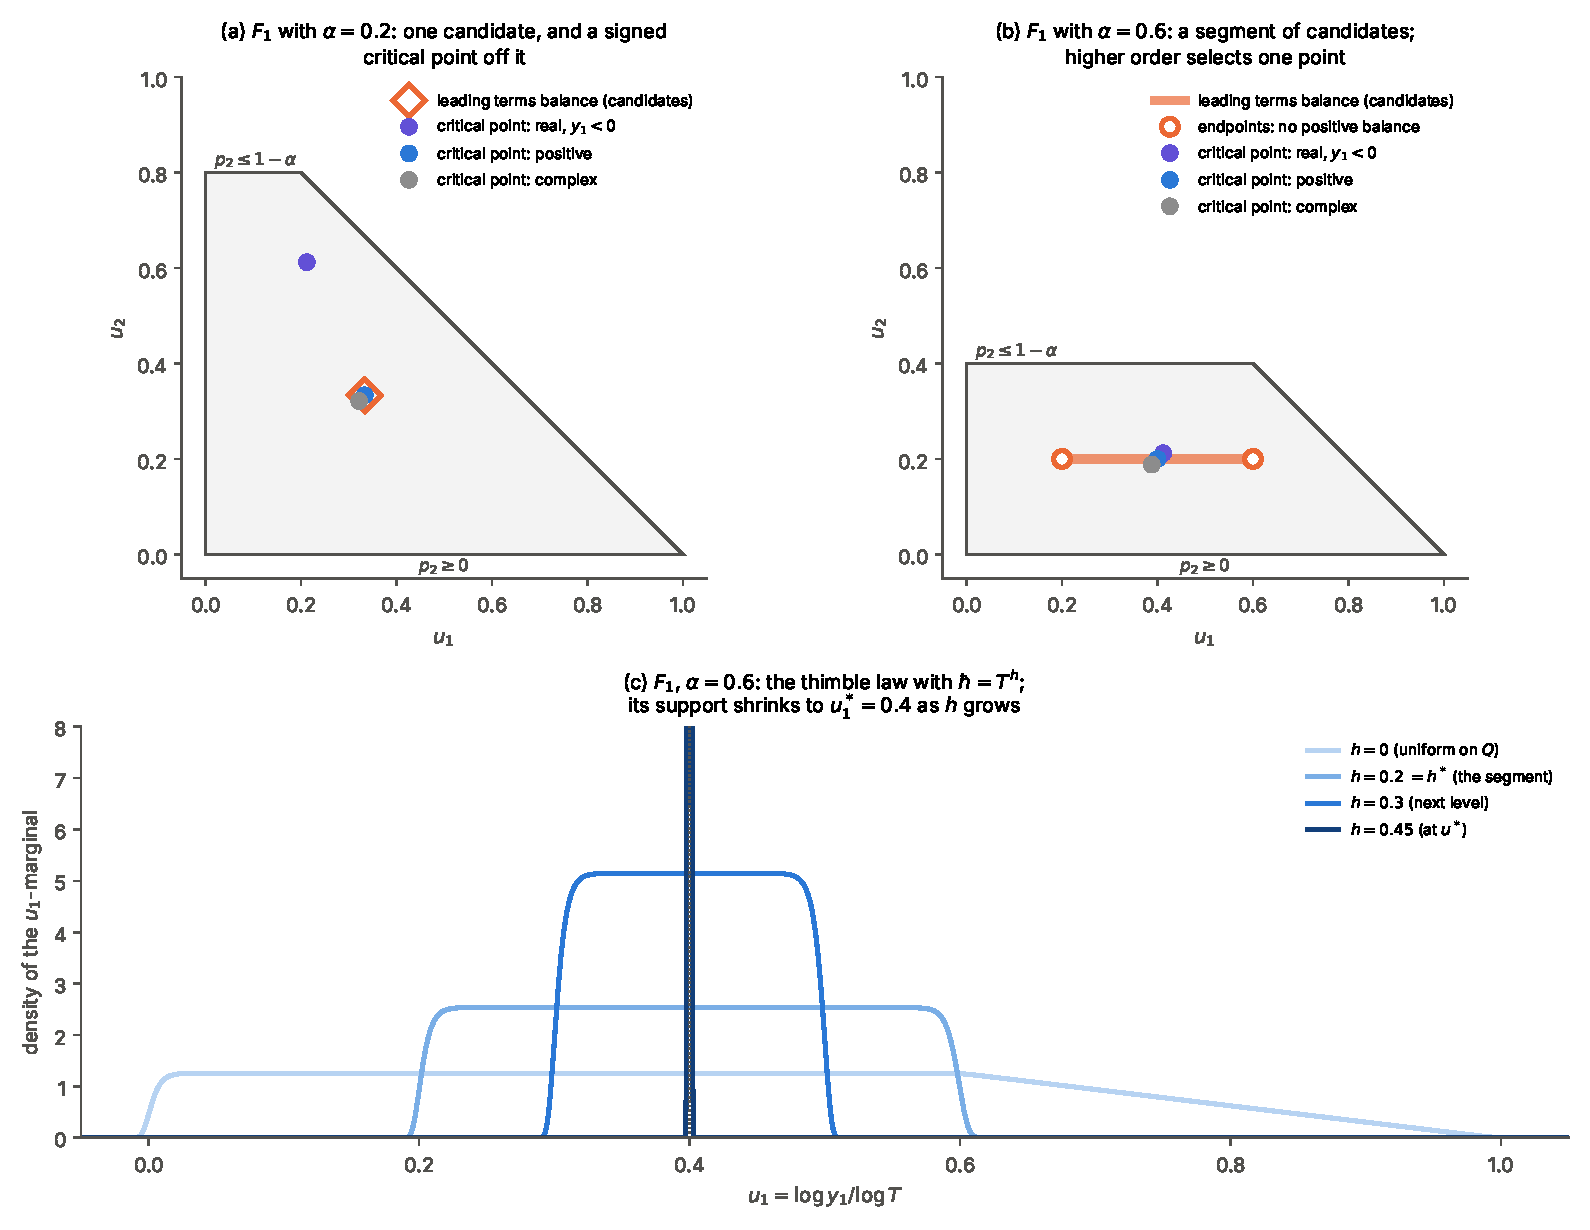
\includegraphics[width=\linewidth]{fig_kahler.pdf}
\caption{$F_1$ at two blow-up sizes. (a) $\alpha=0.2$: the only point where the leading terms balance is the barycentre, which carries the positive critical
point; a real critical point with $y_1<0$ sits over $(\alpha,1-2\alpha)$, outside the positive theory. (b) $\alpha=0.6$: the leading terms balance along an open segment, whose endpoints (open circles) have no positive balance,
and the critical points all sit over one point of it. (c) $\alpha=0.6$: the $u_1$-marginal of the thimble law with $\hbar=T^h$ (\cref{thm:tropical,ex:levels}). At
$h=0$ it is the marginal of the uniform law on $Q$; at $h=h^*=0.2$ it is uniform on the segment; at $h=0.3$ it is uniform on $[0.3,0.5]$; above
$0.4$ it is concentrated at $u_1^*=0.4$. Here $\log T=-200$, and $-100$ for $h=0.45$.}\label{fig:F1}
\end{figure}

\section{The positive thimble and its tropical limit}\label{sec:thimble}
The positive critical point has a second, analytic role: it is the critical point of an oscillatory integral. In mirror symmetry the
integral $\int e^{-W/\hbar}\,dy/y$ over the positive real cycle is the one tied to Galkin's conifold point and to Gamma conjecture~I; under homological mirror symmetry that
cycle is expected to correspond to the structure sheaf \cite{Galkin2014,GGI2016,Iritani2009}. Here we only need its elementary properties, and what
the tropical limit does to the law it carries. Give $(\mathbb C^*)^n$ the flat metric $\sum_j|d\log y_j|^2$, and let $\hbar>0$.

\begin{proposition}[the positive thimble]\label{prop:thimble}
\begin{enumerate}
\item[(1)] The positive orthant $(0,\infty)^n$ is the ascending Lefschetz thimble $J_+$ of $y_T$ for $\operatorname{Re}(W_T/\hbar)$, the set of points whose downward gradient flow
  tends to $y_T$. In $b=\log y$, the Hessian of $\operatorname{Re}W_T(e^{b})$ at $b_T=\log y_T$, in the coordinates $(\operatorname{Re}b,\operatorname{Im}b)$, is $\operatorname{diag}(H,-H)$ with
  $H=\operatorname{Hess}(W_T\circ\exp)(b_T)$ positive definite. So the real directions ascend, and $\operatorname{Im}W_T=0$ on $J_+$.
\item[(2)] $\mu_\hbar=Z^{-1}e^{-W_T(y)/\hbar}\,dy/y$ on $J_+$ is a probability law, and $Z<\infty$.
\item[(3)] \emph{Laplace.} As $\hbar/W_T(y_T)\to0$, the law of $b=\log y$ under $\mu_\hbar$ is asymptotically normal, with mean $b_T$ and covariance $\hbar H^{-1}$.
\end{enumerate}
\end{proposition}

\begin{proof}
(1) $W_T\circ\exp(b)=\sum_kT^{-\lambda_k}e^{\langle v_k,b\rangle}$ is holomorphic, and its restriction to real $b$ is strictly convex and coercive (\cref{thm:bridge}(1)). For a
holomorphic $f$, the Hessian of $\operatorname{Re}f$ in $(\operatorname{Re}b,\operatorname{Im}b)$ is $\operatorname{diag}(H,-H)$ with $H$ the real Hessian, by the Cauchy--Riemann equations. The metric is
real, so the gradient flow of $\operatorname{Re}W_T$ preserves the real locus. There the flow is the gradient flow of a strictly convex, coercive function, and
every orbit tends to $b_T$. So the orthant lies in the stable manifold $J_+$, which is an $n$-ball. The orthant is an $n$-manifold, so it is
open in $J_+$; it is closed in $(\mathbb C^*)^n$, so it is closed in $J_+$. Since $J_+$ is connected, the two are equal.
(2) $W_T>0$ on $J_+$, and $W_T(e^b)\ge c|b|-C$ by positive spanning, so $Z<\infty$. (3) This is Laplace's method at the non-degenerate
minimum $b_T$ of $W_T\circ\exp$; the relative corrections are $O(\hbar/W_T(y_T))$. KB7 corroborates (1) and (3), at $\hbar/W_T(y_T)=10^{-2},10^{-3},10^{-4}$.
\end{proof}

Laplace describes the limit $\hbar\to0$ at fixed $T$. The tropical limit couples the two, $\hbar=T^h$, and reads $y$ on the scale of the
valuation, $u=\log y/\log T$. Since $T^{-\lambda_k}y^{v_k}=T^{\ell_k(u)}$, the pushforward $\nu_{T,h}$ of $\mu_{T^h}$ to $u$ has density proportional to
\[
f_{T,h}(u)=\exp\Bigl(-\sum_kT^{\ell_k(u)-h}\Bigr).
\]
Let $g(u)=\min_k\ell_k(u)$, which is the tropicalisation of $W$ in the min convention. Let $h^*=\max_ug$, and let $Q_h=\{u:g(u)\ge h\}=\{\langle v_k,u\rangle\ge\lambda_k+h\}$, so that $Q_0=Q$.

\begin{theorem}[the tropical limit of the thimble law]\label{thm:tropical}
\begin{enumerate}
\item[(1)] If $h<h^*$, then $\nu_{T,h}$ tends, in total variation, to the uniform law on the polytope $Q_h$. At $h=0$ this is the normalised
  Duistermaat--Heckman measure of $X_Q$.
\item[(2)] If $h\ge h^*$, then $\nu_{T,h}$ concentrates on $Q_{h^*}=\operatorname{argmax}g$: $\nu_{T,h}(U)\to1$ for every open $U\supseteq Q_{h^*}$.
\item[(3)] $\operatorname{argmax}g=\{u:0\in\operatorname{conv}\{v_k:k\in K(u)\}\}$. It is a polytope. It contains every candidate, every $u$ with $0\in\operatorname{relint}\operatorname{conv}\{v_k:k\in K(u)\}$, and
  in particular $u^*$; it can also contain non-candidates. Every $u$ outside it has $g(u)<h^*$. This applies to the valuation of a signed critical point of
  \cref{ex:F1}(a) as well.
\end{enumerate}
\end{theorem}

\begin{proof}
Write $L=\log(1/T)$. Since the $v_k$ positively span, $g(u)\le C-c|u|$, so $h^*$ is finite and attained, and the level sets of $g$ are compact.
(1) For $u$ with $g(u)>h$, every exponent is positive and $f_{T,h}(u)\to1$. Off $Q_h$, some exponent is negative and $f_{T,h}(u)\to0$, and $\partial Q_h$ is null. For $T\le T_0<1$,
$f_{T,h}\le\min(1,\exp(-T_0^{\,g-h}))$, which is integrable. By dominated convergence, $\int f_{T,h}\to\operatorname{vol}Q_h>0$, since $Q_h$ has interior when $h<h^*$. Scheff\'e's lemma then gives
convergence in total variation.
(2) Choose $\delta>0$ with $\{g\ge h^*-2\delta\}\subseteq U$. Put $s=h-h^*\ge0$. Off $U$, $T^{g-h}\ge T^{-(s+2\delta)}$, so $\int_{U^c}f_{T,h}\le C\exp(-\tfrac12T^{-(s+2\delta)})$. Near a
maximiser $u_0$, on the ball of radius $1/(ML)$, where $M=\max|v_k|$, every $\ell_k\ge h^*-1/L$. So $f_{T,h}\ge\exp(-me\,T^{-s})$ there, and the mass of the ball is at least
$cL^{-n}\exp(-me\,T^{-s})$. The ratio of the two bounds tends to $0$, because $T^{-2\delta}\to\infty$.
(3) $g$ is concave and piecewise linear, and its superdifferential at $u$ is $\operatorname{conv}\{v_k:k\in K(u)\}$ \cite[Theorem~23.8]{Rockafellar1970}. A point maximises a concave function iff
$0$ lies in its superdifferential. Candidates satisfy this, and so does $u^*$ by \cref{thm:bridge}(2). This recovers, in our setting, the theorem
of Judd and Rietsch that the tropical critical point maximises the tropicalisation \cite[Thm.~1.2]{JuddRietsch2019}. KB8 corroborates (1)--(3) on $\mathbb{CP}^2$ and
on $F_1$ with $\alpha=\tfrac15$ and $\tfrac35$.
\end{proof}

So the first level of the tropical limit sees exactly the max--min set. That set is the first step of the iterated max--min by which
Fukaya, Oh, Ohta and Ono locate a fibre \cite{FOOO2010}, and of the recursive construction of Judd and Rietsch \cite{JuddRietsch2019}. The selection of $u^*$
inside it is a second-level question.

\begin{example}[the levels on $F_1$]\label{ex:levels}
For $\mathbb{CP}^2$, and for $F_1$ with $\alpha<\tfrac13$, $h^*=\tfrac13$ and $\operatorname{argmax}g$ is the barycentre. The signed fibre of \cref{ex:F1}(a) has $g=\alpha<h^*$. For
$F_1$ with $\alpha>\tfrac13$, $h^*=\tfrac{1-\alpha}2$, and $\operatorname{argmax}g$ is the closed segment $S=\{u_2=\tfrac{1-\alpha}2,\ \tfrac{1-\alpha}2\le u_1\le\alpha\}$. Its relative interior consists of the
candidates, and its endpoints are maximisers that are not candidates.
\begin{enumerate}
\item[(a)] At $h=h^*$ the $u_1$-marginal of $\nu_{T,h}$ tends to the \emph{uniform} law on $[\tfrac{1-\alpha}2,\alpha]$. Leading order gives the selected point no extra mass.
\item[(b)] On $S$, $\ell_1=u_1$ and $\ell_3=\tfrac{1+\alpha}2-u_1$. The next max--min level is $h_2=\max_S\min(\ell_1,\ell_3)=\tfrac{1+\alpha}4$, attained at $u_1=\tfrac{1+\alpha}4=u^*_1$. For
  $h^*<h<h_2$, the $u_1$-marginal tends to the uniform law on $[h,\tfrac{1+\alpha}2-h]$. For $h>h_2$, it concentrates at $u_1^*$.
\end{enumerate}
\emph{Sketch.} Near $S$, the transverse factor $\exp(-T^{u_2-h}-T^{1-\alpha-u_2-h})$ does not depend on $u_1$. The coupling of $u_2$ to $\ell_3$ matters only in boundary layers of width
$O(1/L)$. So the $u_1$-marginal behaves as in \cref{thm:tropical}, now for $\min(\ell_1,\ell_3)$ on $S$.
KB8 corroborates (a) and (b) for $\alpha=\tfrac35$, at $h=\tfrac15,\tfrac3{10},\tfrac9{20}$ (\cref{fig:F1}(c)). That the mean at level $h^*$ equals $u_1^*$ here is a symmetry of this
example: $u^*_1$ is the midpoint of $S$. The mechanism of selection is the second level, not the mean.
\end{example}

\section{Soft evidence moves \texorpdfstring{$\lambda$}{lambda}}\label{sec:data}
This section starts the programme of conditioning existing structures on data and recording what changes. It treats one kind of data,
soft evidence whose strength grows with the amount of data. Hard evidence (zero cells) and forgetting are not treated here.

\begin{definition}[the data action]\label{conv:data}
Fix a reference scale $N$ and put $T=e^{-N}$. Evidence that multiplies term $k$ of $W_T$ by $e^{-n\rho_k}$ after $n$ observations, with rates $\rho_k\ge0$, multiplies it by
$T^{(n/N)\rho_k}$. So it replaces $\lambda$ by
\[
\lambda^{\mathrm{eff}}=\lambda-s\rho,\qquad s=n/N .
\]
Which term each observation weighs, and the scale $N$, are modelling choices. A likelihood of fixed size has $s\to0$ as $N\to\infty$. It changes the
coefficients smoothly, as in \cref{prop:kahler}, and changes no valuation.
\end{definition}

Let $\Delta_m$ be the laws on the $m$ facets, and let $B=\{q\in\Delta_m:\sum_kq_kv_k=0\}$ be the \emph{balance polytope}, the laws with mean exponent $0$. It has dimension $m-n-1$,
because $0$ lies in the interior of $\operatorname{conv}\{v_k\}$. Write $g_\lambda=\min_k\ell_k$, $h^*(\lambda)=\max g_\lambda$, and $F(\lambda)$ for the face of $B$ on which $\langle q,\lambda\rangle$ is maximal.

\begin{proposition}[the max--min level is a balance programme]\label{prop:balancelp}
\begin{enumerate}
\item[(1)] $h^*(\lambda)=\min_{q\in B}\bigl(-\langle q,\lambda\rangle\bigr)$. So $h^*$ is concave and piecewise linear in $\lambda$.
\item[(2)] Let $K_0$ be the union of the supports of the laws in $F(\lambda)$, and $\sigma_0=\operatorname{conv}\{v_k:k\in K_0\}$. Then $K(u)=K_0$ on the relative interior of $\operatorname{argmax}g_\lambda$, and
  $K(u)\supsetneq K_0$ on its relative boundary. The candidates (\cref{thm:tropical}(3)) are exactly the relative interior, and $\dim\operatorname{argmax}g_\lambda=n-\dim\sigma_0$.
\item[(3)] The limit law of the positive critical point (\cref{thm:bridge}(2)) lies in $F(\lambda)$.
\end{enumerate}
\end{proposition}

\begin{proof}
(1) $\max_u\min_k\ell_k=\max_u\min_{q\in\Delta_m}\sum_kq_k\ell_k(u)$, and the minimax theorem exchanges the two. For fixed $q$, $\sup_u\sum_kq_k(\langle v_k,u\rangle-\lambda_k)$ is $-\langle q,\lambda\rangle$ if $\sum_kq_kv_k=0$
and $+\infty$ otherwise. (2) By complementary slackness, $q_k>0$ for an optimal $q$ forces $\ell_k(u)=h^*$ at every maximiser $u$, so $K(u)\supseteq K_0$ on $\operatorname{argmax}g_\lambda$. By strict
complementarity \cite{Schrijver1986}, some maximiser has $\ell_j>h^*$ for every $j\notin K_0$. The same then holds on the relative interior of $\operatorname{argmax}g_\lambda$, which is
$\{u:\ell_k(u)=h^*\ (k\in K_0),\ \ell_j(u)>h^*\ (j\notin K_0)\}$. A law in the relative interior of $F(\lambda)$ is positive on $K_0$ and has mean $0$, so those points are candidates (\cref{lem:balance}). At a
boundary point, suppose $0$ were in the relative interior of $\operatorname{conv}\{v_k:k\in K(u)\}$. Then there would be a balanced law positive on all of $K(u)$. That law would be optimal,
since $\sum_kq_k\ell_k(u)=h^*$, so its support would lie in $K_0$, a contradiction. The linear span of $\{v_k:k\in K_0\}$ is its affine span, since it contains $0$, so the equations $\ell_k=h^*$ on $K_0$ cut out
dimension $n-\dim\sigma_0$. (3) The limit law $q$ is balanced and supported on $K(u^*)$, where every $\ell_k(u^*)=h^*$. So $-\langle q,\lambda\rangle=\sum_kq_k\ell_k(u^*)=h^*$, and $q$ is optimal.
DW2 and DW3 corroborate (1)--(3) on $40$ and $23$ configurations.
\end{proof}

So candidates against selection appears twice, in dual spaces. In $u$-space, $u^*$ is selected inside the relative interior of $\operatorname{argmax}g_\lambda$, which has dimension $n-\dim\sigma_0$. In law space, the
limit law is selected inside $F(\lambda)$. The two can be non-trivial at different parameters (\cref{ex:F1wall}).

\begin{corollary}[where data can act]\label{cor:where}
\begin{enumerate}
\item[(1)] The leading set $K_0$, the candidate dimension and the face $F$ change only on the walls of the normal fan of $B$, the \emph{outcome walls}. Within a
  chamber, $h^*$ is affine in $\lambda$, and so is $u^*$ when $\sigma_0$ is an $n$-simplex.
\item[(2)] Evidence along a translation, $\rho_k=\langle v_k,t\rangle$, changes nothing but $u^*\mapsto u^*-st$. Evidence along the constant, $\rho=\mathbf 1$, changes nothing but $h^*\mapsto h^*+s$. Only the quotient of $\R^m$ by these
  $n+1$ directions can cross a wall. It has dimension $m-n-1$, the number of independent affine dependences (circuits) of $\{v_k\}$.
\item[(3)] Suppose there is one circuit $a$, normalised to be primitive and integral. The wall is $c(\lambda)=-\langle a,\lambda\rangle=0$, and along $\lambda_0-s\rho$ it is reached at
  $s^*=-c(\lambda_0)/\langle a,\rho\rangle$ when this is positive, never otherwise. Over rates with $\max_k\rho_k-\min_k\rho_k\le1$, the least such $s$ is $|c(\lambda_0)|/(\tfrac12\|a\|_1)$.
\end{enumerate}
\end{corollary}

\begin{proof}
(1) $F(\lambda)$ is constant on the relative interior of each cone of the normal fan of $B$; apply \cref{prop:balancelp}. On a chamber, $h^*=-\langle q_0,\lambda\rangle$ for a fixed vertex $q_0$. When $\sigma_0$ is an
$n$-simplex, $u^*$ is the unique solution of $\ell_k(u)=h^*$, $k\in K_0$, which is linear in $\lambda$. (2) Under a translation, $\ell_k$ becomes $\ell_k(u+st)$. Under the constant, every $\ell_k$ shifts by $s$.
Both are orthogonal to $B-B$, which consists of affine dependences. (3) $B$ is a segment, and its normal fan has one wall, $\langle q_A-q_B,\lambda\rangle=0$, where $q_A-q_B$ is a multiple of $a$.
Since $\sum_ka_k=0$, adding a constant to $\rho$ leaves $\langle a,\rho\rangle$ unchanged. So the best value over range at most $1$ is $\sum_ka_k^+=\tfrac12\|a\|_1$.
\end{proof}

\begin{example}[$\mathbb{CP}^2$: no wall]
Here $m=n+1$, so there is no circuit, and $B$ is the single law $(\tfrac13,\tfrac13,\tfrac13)$. No soft evidence changes the leading set of $\mathbb{CP}^2$. Data only move the selected point and the level
(DW4, DW7).
\end{example}

\begin{example}[$F_1$ across its wall]\label{ex:F1wall}
For general $\lambda$, put $L=-(\lambda_1+\lambda_2+\lambda_3)$ and $\alpha=-\lambda_1-\lambda_3+\lambda_4$. These are the size of the triangle and the length of the blown-up facet, and both are
invariant under translation. The K\"ahler cone is $0<\alpha<L$. Its walls are viability walls, where the polytope loses facet~$4$ or collapses, and $X_Q$ changes.
The one circuit is $a=(2,-1,2,-3)$, with $c(\lambda)=3\alpha-L$. The balance polytope is the segment from $q_A=(\tfrac13,\tfrac13,\tfrac13,0)$ to $q_B=(0,\tfrac12,0,\tfrac12)$, and $h^*=\min\bigl(L/3,(L-\alpha)/2\bigr)$.
\begin{enumerate}
\item[(a)] The outcome wall $\alpha=L/3$ lies \emph{inside} the K\"ahler cone: the manifold does not change there. Below it, $K_0=\{1,2,3\}$ and the candidate is a point.
  Above it, $K_0=\{2,4\}$, the candidates form an open segment, and $u^*$ is selected at the second level (\cref{ex:levels}). The lower diagonal of the subdivision flips from $v_1v_3$ to $v_2v_4$.
\item[(b)] $u^*$ is continuous and piecewise affine across the wall (\cref{fig:data}(a)). What jumps is the leading set, the candidate dimension ($0\to1$) and the mechanism of
  selection (leading order $\to$ second level). The signed fibre over $(\alpha,1-2\alpha)$ reaches the barycentre at the wall. By the cited theorem \cite{ChoOh2006}, the number of
  torus fibres with non-vanishing Floer cohomology drops from two to one there. We claim nothing about the Fukaya category.
\item[(c)] \emph{At the wall} ($\alpha=1/3$, $L=1$), the substitution $w=T^{1/6}x$ turns the quartic of \cref{ex:F1} into $x^4-x-1=0$ for every $T$. So the positive law is
  $(1/x,\,x^2,\,1/x,\,1/x^2)/\Sigma\approx(0.2156,0.3922,0.2156,0.1766)$ for every $T$, where $x\approx1.2207$. It is the interior point $(1-t)q_A+tq_B$ of $F=B$, with $t\approx0.353$. Here the candidate in
  $u$-space is a single point, but the law is selected inside a segment.
\item[(d)] The discriminant of $w^4-T^{1/2}w-T^{1-\alpha}$ is $-27T^2-256T^{3-3\alpha}$, which never vanishes: no two critical points collide for $T>0$. The outcome wall is where
  its two terms have equal order. It is a wall of the tropical discriminant, not of the discriminant itself.
\item[(e)] \emph{Data.} Start at $\alpha=1/5$, $L=1$, so $c=-2/5$. Evidence against term~$1$, $\rho=e_1$, has $\langle a,\rho\rangle=2$ and reaches the wall at $s^*=1/5$, that is $n^*=N/5$
  (\cref{fig:data}(b)). Along the way $\alpha/L=(1/5+s)/(1+s)$ stays in the K\"ahler cone. Evidence against term~$4$ ($\langle a,\rho\rangle=-3$) never reaches the wall. The most efficient
  rates with range at most $1$ are $\rho=(1,0,1,0)$, against terms $1$ and $3$, with $s=1/10$.
\end{enumerate}
DW4--DW7 corroborate (a)--(e).
\end{example}

\begin{figure}[!htbp]\centering
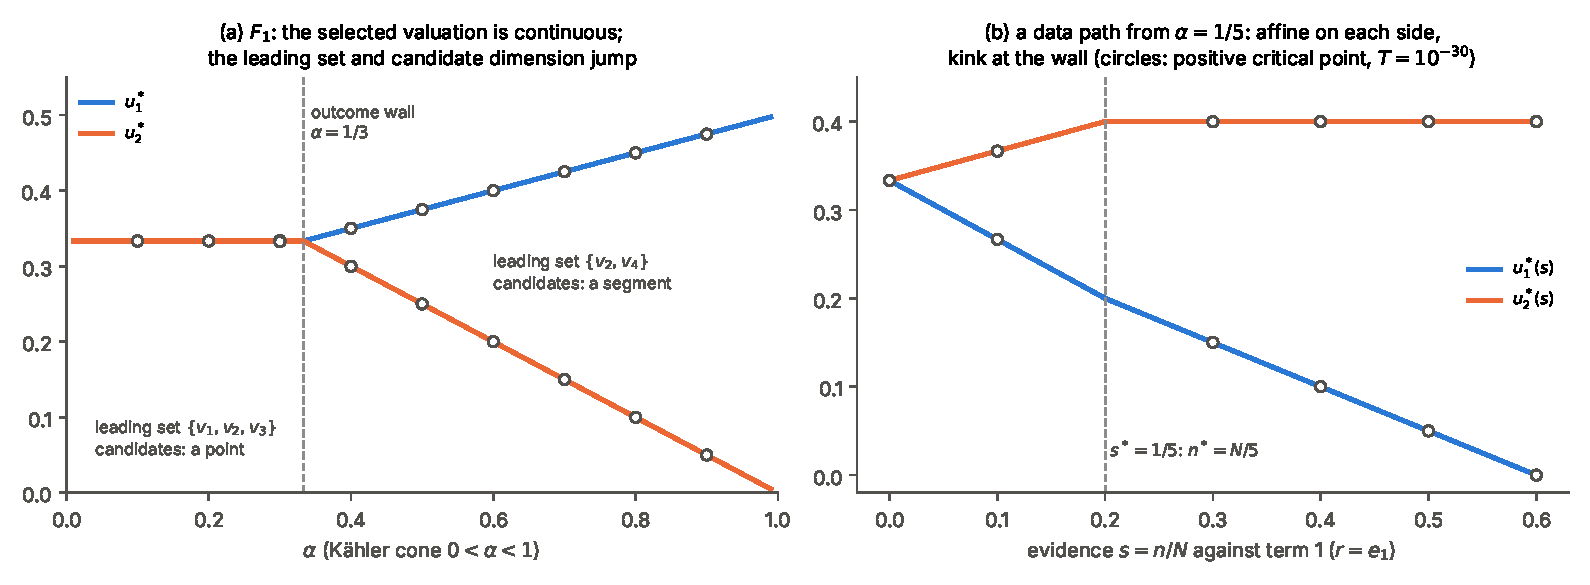
\includegraphics[width=\linewidth]{fig_datawalls.pdf}
\caption{Soft evidence on $F_1$. (a) The selected valuation $u^*$ across the K\"ahler cone. The curves are the chamber formulas and the circles the positive critical point at
$T=10^{-30}$. The outcome wall at $\alpha=1/3$ changes the leading set and the candidate dimension, not the position of $u^*$; here $h^*=u_2^*$. (b) A data path from $\alpha=1/5$ with evidence
against term~$1$: $u^*(s)$ is affine on each side of $s^*=1/5$, with a kink at the wall.}\label{fig:data}
\end{figure}

On $F_1$, then, the least data that changes the perspective changes \emph{which terms carry the limit law}, not where the selected state
sits. A decision that reads the leading set jumps at $n^*$. A decision that reads $u^*$ continuously does not. Decision, contextuality and
value-of-information walls need their own definitions, a decision model, a named complex and obstruction class, and an information-acquisition
model, before they can be compared with the outcome walls. We record them separately and have not computed them.

\part{Back to contingency tables}
Part~I went from toric geometry to conditioned probability. Part~II runs the dictionary backwards, from a table of counts to the potential,
and asks what the Floer-selected fibre means for the table. It works the independence model exactly. Every operation it uses, and every
operation it does not yet treat, is recorded in the ledger (\cref{app:ledger}).

\section{Two configurations of one model}\label{sec:twoconf}
An $r\times c$ table of counts $t_{ij}$ has row margins $t_{i+}$ and column margins $t_{+j}$. The independence model is the log-linear model whose design
matrix $A$ has one column per cell, the row indicator stacked on the column indicator. It is toric \cite{DiaconisSturmfels1998,GeigerMeekSturmfels2006}: its sufficient
statistic is the vector of margins, and by Birch the MLE is the unique law in the model with the observed margins, $\hat p_{ij}=t_{i+}t_{+j}/n^2$
\cite{Birch1963,BishopFienbergHolland1975}. The moment polytope of this model is $\Delta_{r-1}\times\Delta_{c-1}$, so its manifold is $\mathbb{CP}^{r-1}\times\mathbb{CP}^{c-1}$, which is Delzant and Fano.

The model carries two different point configurations, and they must not be confused.
\begin{proposition}[cells and facets]\label{prop:twoconf}
\begin{enumerate}
\item[(1)] \emph{Cells.} The $rc$ columns of $A$ satisfy $(r-1)(c-1)$ independent linear relations. These are spanned by the basic moves $+1$ at $(i,j),(k,l)$ and $-1$ at $(i,l),(k,j)$,
  which change a table without changing its margins. This is the Tier~A support of \cref{prop:kahler}.
\item[(2)] \emph{Facets.} The $r+c$ inward facet normals of $\Delta_{r-1}(L_1)\times\Delta_{c-1}(L_2)$ have exactly one circuit, $a=(c\,\mathbf 1_r,-r\,\mathbf 1_c)/\gcd(r,c)$. This is the configuration $W$ is built from.
\end{enumerate}
\end{proposition}

\begin{proof}
(1) $A$ has rank $r+c-1$, and the moves lie in its kernel and have rank $(r-1)(c-1)$ \cite{DiaconisSturmfels1998}. (2) $m-n-1=(r+c)-(r+c-2)-1=1$. The row normals sum to $0$, and
so do the column normals. So $\sum_ka_kv_k=0$, and $\sum_ka_k=rc-cr=0$. CT1 checks both for $r,c\in\{2,3,4\}$.
\end{proof}

So the $2\times3$ model has two moves but one circuit. The moves act on tables with fixed margins, within a fibre. The circuit acts on
$\lambda$, across K\"ahler classes. The second statement is a special case of a general count.

\begin{proposition}[products add one circuit]\label{prop:product}
If $v^{(1)}$ and $v^{(2)}$ both have $0$ in the interior of their convex hulls, the product configuration has $(m_1-n_1-1)+(m_2-n_2-1)+1$ independent circuits. The extra
one is $(q^{(1)},-q^{(2)})$ for balanced laws $q^{(i)}$ of the factors. Its wall is $h^*_1=h^*_2$ when each factor has a single balanced law.
\end{proposition}

\begin{proof}
The count is $(m_1+m_2)-(n_1+n_2)-1$. The vector $(q^{(1)},-q^{(2)})$ sums to $1-1=0$, and both halves balance. It is independent of the circuits of the factors,
which sum to zero on each factor separately. When $B_i=\{q^{(i)}\}$, the balance programme gives $h^*=\min(h_1^*,h_2^*)$ (\cref{prop:balancelp}), with a wall where they are equal.
\end{proof}

\section{The independence model: its wall and its selection}\label{sec:indep}
In the coordinates $b$ = the first $r-1$ row margins and the first $c-1$ column margins, the facets of $Q=\Delta_{r-1}(L_1)\times\Delta_{c-1}(L_2)$ have $\ell_k(b)$ equal to the $k$-th
margin. Here $L_1$ and $L_2$ are the totals of the row and column margins. So $W=W_{\mathrm{row}}(y)+W_{\mathrm{col}}(z)$ with $W_{\mathrm{row}}=y_1+\dots+y_{r-1}+T^{L_1}/(y_1\cdots y_{r-1})$, and similarly for columns.

\begin{theorem}[the independence model]\label{thm:indep}
\begin{enumerate}
\item[(1)] $h^*=\min(L_1/r,\,L_2/c)$. The leading set is the row facets if $cL_1<rL_2$, the column facets if $cL_1>rL_2$, and all $r+c$ facets on the wall $cL_1=rL_2$.
  The wall is $c(\lambda)=-\langle a,\lambda\rangle=(cL_1-rL_2)/\gcd(r,c)=0$.
\item[(2)] The critical points of $W$ are $y_i=\zeta T^{L_1/r}$, $z_j=\eta T^{L_2/c}$ with $\zeta^r=\eta^c=1$, so there are $rc$ of them. All have the valuation $u^*=(L_1/r,\dots;L_2/c,\dots)$, the
  uniform margins, for every $L_1,L_2$. The positive law is exactly proportional to $T^{L_1/r}$ on each row facet and $T^{L_2/c}$ on each column facet.
\item[(3)] Off the wall the candidates have dimension $c-1$ (if $cL_1<rL_2$) or $r-1$, and the uniform margins are selected at the second level. On the wall the candidate
  is the single point $u^*$.
\item[(4)] By the cited theorem \cite{ChoOh2006}, exactly one torus fibre has non-vanishing Floer cohomology, for every $L_1,L_2$. So the outcome wall of the independence
  model changes no Floer data. On $F_1$ it does (\cref{ex:F1wall}(b)).
\end{enumerate}
\end{theorem}

\begin{proof}
(1) Each factor has the single balanced law, uniform on its facets, with values $L_1/r$ and $L_2/c$. Apply \cref{prop:product}. (2) The variables separate.
$\partial W_{\mathrm{row}}/\partial y_i=0$ gives $y_i\prod_jy_j=T^{L_1}$ for every $i$, so all $y_i$ are equal and $y^r=T^{L_1}$. The term values are then $T^{L_1/r}$ times a root of unity. (3) Off the
wall the leading set is one factor's facets, so $\sigma_0$ has dimension $r-1$ (or $c-1$); apply \cref{prop:balancelp}(2). (4) All critical points share one valuation.
CT2 and CT3 check (1)--(3), with exact rationals and gradients.
\end{proof}

\section{Margins against evidence}\label{sec:margins}
Data enter in two ways, and the note keeps them apart.

\begin{proposition}[two roles of data]\label{prop:roles}
\begin{enumerate}
\item[(1)] \emph{Observed margins} $b$ pick a point of $Q$, the fibre $\mu^{-1}(b)$ and the MLE (Birch). For the independence model, $\ell_k(b)$ is exactly the $k$-th margin, the facet
  $\{\ell_k=0\}$ is a zero margin, and the MLE lies in the open model iff every margin is positive \cite{BishopFienbergHolland1975}. For general hierarchical models the
  facets correspond to facial sets of cells, and the MLE fails to exist exactly when the margins lie on a proper face \cite{EFRS2006,FienbergRinaldo2012}. We use only the independence case.
\item[(2)] \emph{Evidence on the terms of $W$} moves $\lambda$ (\cref{conv:data}), and with it $u^*$, $h^*$ and the walls. With $\lambda$ fixed, $u^*$ does not depend on $b$.
\item[(3)] Both $b$ and $u^*$ are points of $Q$, in moment coordinates. The valuation of a critical point is the moment coordinate of its torus fibre $L(u^*)=\mu^{-1}(u^*)$
  \cite{ChoOh2006}. So the MLE fibre and the Floer-selected fibre can be compared in one space. For the independence model we use the Fisher--Rao distance within
  the model, between $\hat p$ and the law at $u^*$ (uniform margins). With surveys of sizes $n_1$ for rows and $n_2$ for columns,
  \[
  d(\hat p,p^*)^2=n_1\,d_\Delta(\hat p_{\mathrm{row}},\mathbf 1/r)^2+n_2\,d_\Delta(\hat p_{\mathrm{col}},\mathbf 1/c)^2,\qquad d_\Delta(p,q)=2\arccos\sum_i\sqrt{p_iq_i}.
  \]
  Joint sampling of $n$ cells is the case $n_1=n_2=n$. A coarser index is the \emph{centrality} $g(b)/h^*$: the smallest margin divided by its largest possible value.
\end{enumerate}
\end{proposition}

\begin{proof}
(1) The first statements are direct, and the MLE formula shows positivity. (2) is \cref{cor:where} together with the fact that $W$ does not involve $b$. (3) The Fisher
information of the independence family is block diagonal, $n_1\operatorname{Cov}(\mathrm{row})\oplus n_2\operatorname{Cov}(\mathrm{col})$, because the log-likelihood separates into a row part and a column
part. So the model is a Riemannian product of two scaled simplices, and on each simplex the Fisher--Rao distance is $2\arccos$ of the Bhattacharyya coefficient \cite{AmariNagaoka2000}.
CT4 and CT5 check (1) and the block structure.
\end{proof}

The MLE fibre and the Floer-selected fibre coincide exactly when the margins are uniform. That the Floer fibre is the uniform-margin table,
the one farthest from every zero-margin degeneracy in lattice distance, is a reading of the cited theorem, not a new statistical result.
The polytope used here is the \emph{base}, the space of margins. \Cref{sec:fibre} turns to the \emph{fibre} over a point of it, the coupling polytope, where the
same margins become the K\"ahler class.

\section{Data and walls in the independence model}\label{sec:indepdata}
\begin{example}[$2\times2$ and $2\times3$]\label{ex:2x3}
Under joint sampling, $L_1=L_2=n$. The $2\times2$ table therefore sits on its wall for every $n$, which is the monotone $\mathbb{CP}^1\times\mathbb{CP}^1$. For $2\times3$, $cL_1-rL_2=n>0$, so $h^*=n/3$, the column
facets lead, and the candidates are the open segment of row margins $b_1\in(n/3,2n/3)$ with uniform column margins. Its endpoints are maximisers but not candidates.
The selected point is $b_1=n/2$. To reach the wall the column survey must grow to $n_2=3n/2$: $n/2$ more column observations. In the terms of \cref{cor:where}(3), this is
$\rho$ on a column facet with $\langle a,\rho\rangle=-r/\gcd$, so $s^*=n/2$. Crossing it changes the leading set and the candidate dimension. By \cref{thm:indep}(4) it changes no Floer data.
CT6 checks every number.
\end{example}

\begin{example}[hard evidence: a structural zero]\label{ex:zero}
Declare cell $(2,2)$ of the $2\times2$ table structurally zero. This is the quasi-independence model on three cells. The three remaining cells span a unimodular
triangle, which is \emph{not} a face of the square: hard evidence need not restrict to a toric divisor. Its facet configuration is that of $\mathbb{CP}^2$, which has no circuit,
so the one wall of the $2\times2$ model is gone. CT7 checks this. The general case, deleting cells of larger tables, is open.
\end{example}

\section{One coupling polytope through every layer}\label{sec:fibre}
\begin{center}\colorbox{stAdapted!60}{\begin{minipage}{0.94\linewidth}\small
\textbf{What this section shows, in plain words.} Fix two margins, a row law $f$ and a column law $g$. The tables (couplings) with those margins form a
polygon, the \emph{fibre}. That polygon is the picture of a toric surface, and everything in Part~I can be drawn on it.
\begin{itemize}[leftmargin=1.4em,itemsep=1pt]
\item The usual conditional law of a table given its margins, the one behind Fisher's exact test, \emph{is} the toric K\"ahler structure (\cref{fig:cpltierA}).
\item The positive critical point of $W$ picks the \emph{leximin} coupling: the one whose smallest cell is as large as possible (\cref{fig:cplglance}).
\item The positive thimble is a family of laws on couplings. It runs from ``every coupling equally likely'' to ``only the leximin coupling'' (\cref{fig:cplthimble}).
\item Two kinds of wall cut the space of margins. Blow-up walls change the surface; leximin walls change which cells lead. Here one count of
  data crosses a leximin wall and changes the Floer fibres, while the surface stays the same (\cref{fig:cplwalls}).
\end{itemize}
The example is the one followed in the architecture note \cite{Awasthi2026Arch}: $f=(2/5,3/5)$, $g=(3/10,43/100,27/100)$.
\end{minipage}}\end{center}

\subsection{Base and fibre}
A pair of margins is a point of the \emph{base}, $\Delta_{n-1}\times\Delta_{m-1}$ (\cref{sec:indep}). Over it sits the \emph{fibre}, the coupling polytope $\mathrm{Cpl}(f,g)$ of tables with those
margins. For nondegenerate margins the fibre is Delzant, its facets are cells $\{\alpha_c=0\}$, and the K\"ahler class of its toric manifold is the product coupling,
$[\omega_{f,g}]=\sum_cf_ig_j[D_c]$ \cite{Awasthi2026Cpl}. So the same data play two roles:
\begin{center}\small
\begin{tabular}{lll}\toprule
 & base (\cref{sec:twoconf,sec:indep,sec:margins}) & fibre (this section)\\\midrule
points & margins $(f,g)$ & couplings $\alpha$ with those margins\\
facets & a zero margin & a zero cell\\
the margins are & a point (the Birch/MLE fibre) & the K\"ahler class: $\lambda_c$ is read off $(f,g)$\\
$W$ is a sum over & margin facets & cell facets\\
Tier~A support & cells, with $(r-1)(c-1)$ moves & integer tables with these margins\\\bottomrule
\end{tabular}
\end{center}
For $2\times3$, write a coupling by $x=\alpha_{11}$, $y=\alpha_{12}$. Then $\alpha_{13}=f_1-x-y$, $\alpha_{21}=g_1-x$, $\alpha_{22}=g_2-y$ and $\alpha_{23}=x+y-(f_1+g_1+g_2-1)$, so cell $c$ has $\ell_c=\langle v_c,(x,y)\rangle-\lambda_c$ with
$v_c\in\{(1,0),(0,1),(-1,-1),(-1,0),(0,-1),(1,1)\}$.

\begin{example}[the fibre]\label{ex:pentagon}
For $f=(2/5,3/5)$, $g=(3/10,43/100,27/100)$ the fibre is the pentagon with vertices $(13/100,0)$, $(3/10,0)$, $(3/10,1/10)$, $(0,2/5)$, $(0,13/100)$ and area $1331/20000$, so $X=\mathrm{Bl}_2\mathbb{CP}^2$.
Its facets are the cells $11,12,13,21,23$. Cell $22$ never vanishes, since $\alpha_{22}\ge f_2+g_2-1=3/100$. Scaled by $n=100$, its lattice points are the $715$ integer tables with
margins $(40,60)$ and $(30,43,27)$. By Pick's theorem, $715=665.5+97/2+1$. CF1 and CF2 check this exactly.
\end{example}

\begin{figure}[!htbp]\centering
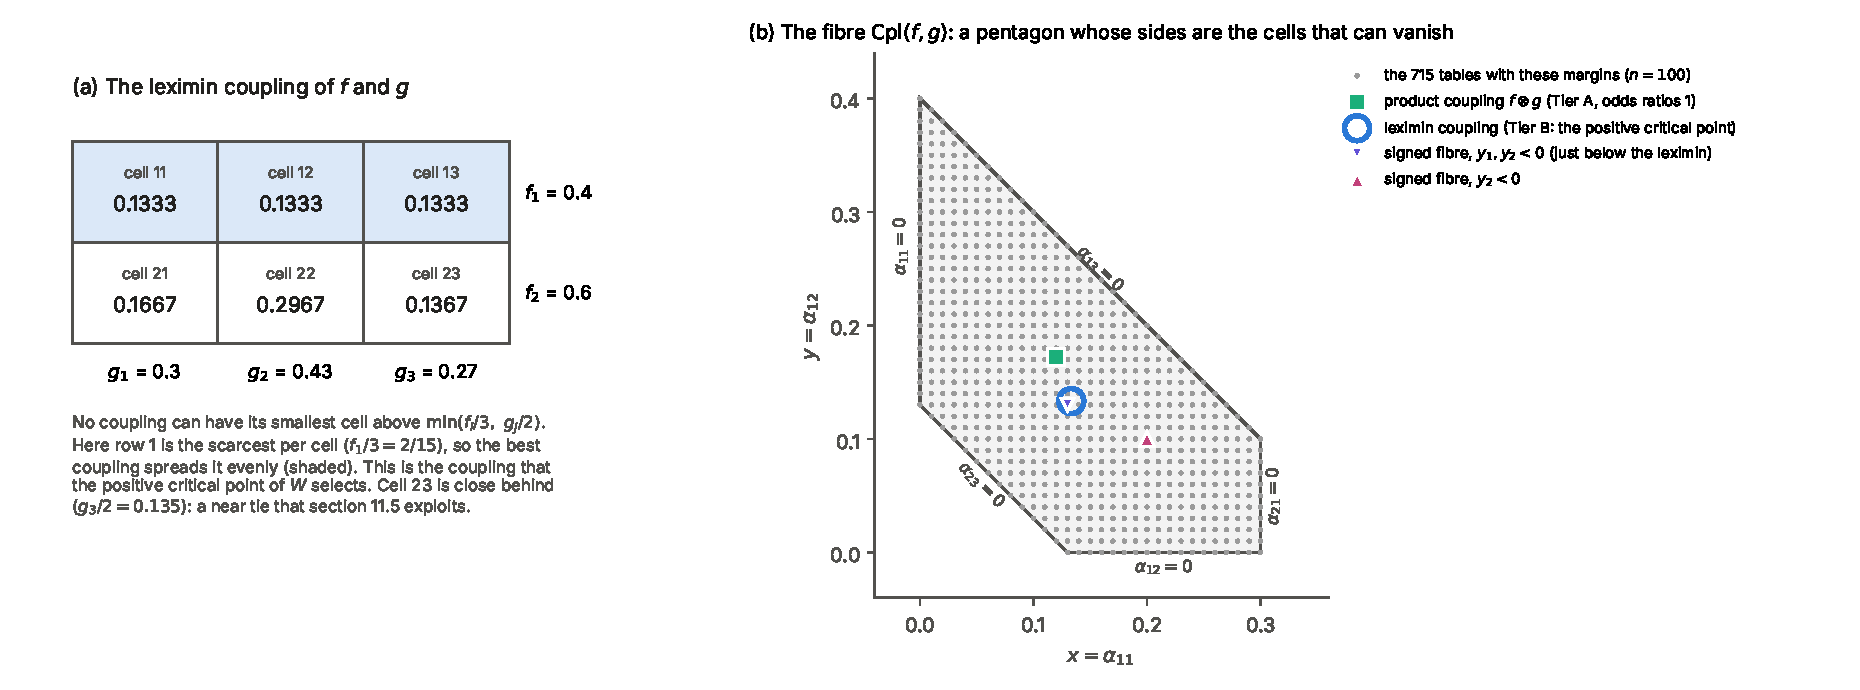
\includegraphics[width=\linewidth]{fig_cpl_glance.pdf}
\caption{The example at a glance. (a) The leximin coupling: row~1 is the scarcest per cell, so it is spread evenly, and every other cell is larger. (b) The fibre,
with the $715$ tables as dots. Each side is a cell that can vanish. Marked: the product coupling, selected by Tier~A; the leximin coupling, selected by the positive
critical point of $W$; and the two real critical points with a negative coordinate (signed fibres).}\label{fig:cplglance}
\end{figure}

\subsection{Tier A on the fibre is Fisher's noncentral hypergeometric family}
\begin{proposition}[the conditional law of a table]\label{prop:hypergeom}
Let $S$ be the integer tables with margins $Nf$, $Ng$, written by $(t_{11},t_{12})$, with weights $c_t=1/\prod_{ij}t_{ij}!$.
\begin{enumerate}
\item[(1)] For any cell parameters $\theta_{ij}>0$, the law of a table under independent Poisson (or multinomial) sampling with means $\propto\theta_{ij}$, conditioned on its margins,
  is the monomial law $q(u)\propto c_t\,e^{\langle u,(t_{11},t_{12})\rangle}$. Here $u_1=\log\frac{\theta_{11}\theta_{23}}{\theta_{13}\theta_{21}}$ and $u_2=\log\frac{\theta_{12}\theta_{23}}{\theta_{13}\theta_{22}}$ are the two log odds ratios. This is Fisher's noncentral
  hypergeometric family. At $u=0$ it is the central hypergeometric law, the null law of Fisher's exact test \cite{Fisher1935}.
\item[(2)] By \cref{prop:kahler}, $\varphi(u)=\log\sum_tc_te^{\langle u,t\rangle}$ is a K\"ahler potential. The moment map is the expected table, and the K\"ahler metric is the Fisher information of the odds ratios. Since $S$ is
  the set of lattice points of the Delzant lattice polygon $N\cdot\mathrm{Cpl}(f,g)$, the form extends to all of $X=\mathrm{Bl}_2\mathbb{CP}^2$.
\item[(3)] At $u=0$ the mean is exactly $N\,f\otimes g$: Tier~A at odds ratios $1$ selects the product coupling.
\item[(4)] Every interior coupling is the mean for exactly one $u$ (Birch). In the example, the leximin coupling needs odds ratios $(e^{u_1},e^{u_2})\approx(0.82,0.46)$.
\end{enumerate}
\end{proposition}

\begin{proof}
(1) $\prod_{ij}\theta_{ij}^{t_{ij}}/t_{ij}!$ restricted to fixed margins depends on $t$ only through $c_t$ and $t_{11}u_1+t_{12}u_2$. Substituting $t_{13},t_{21},t_{22},t_{23}$ from the margins
gives the two log odds ratios. (2) is \cref{prop:kahler} and its compact case. (3) The central hypergeometric mean is $t_{i+}t_{+j}/N$ \cite{BishopFienbergHolland1975}. (4) is
\cref{prop:kahler}(3). CF3 checks (1) and (3), the latter in exact rationals, and computes (4).
\end{proof}

\begin{figure}[!htbp]\centering
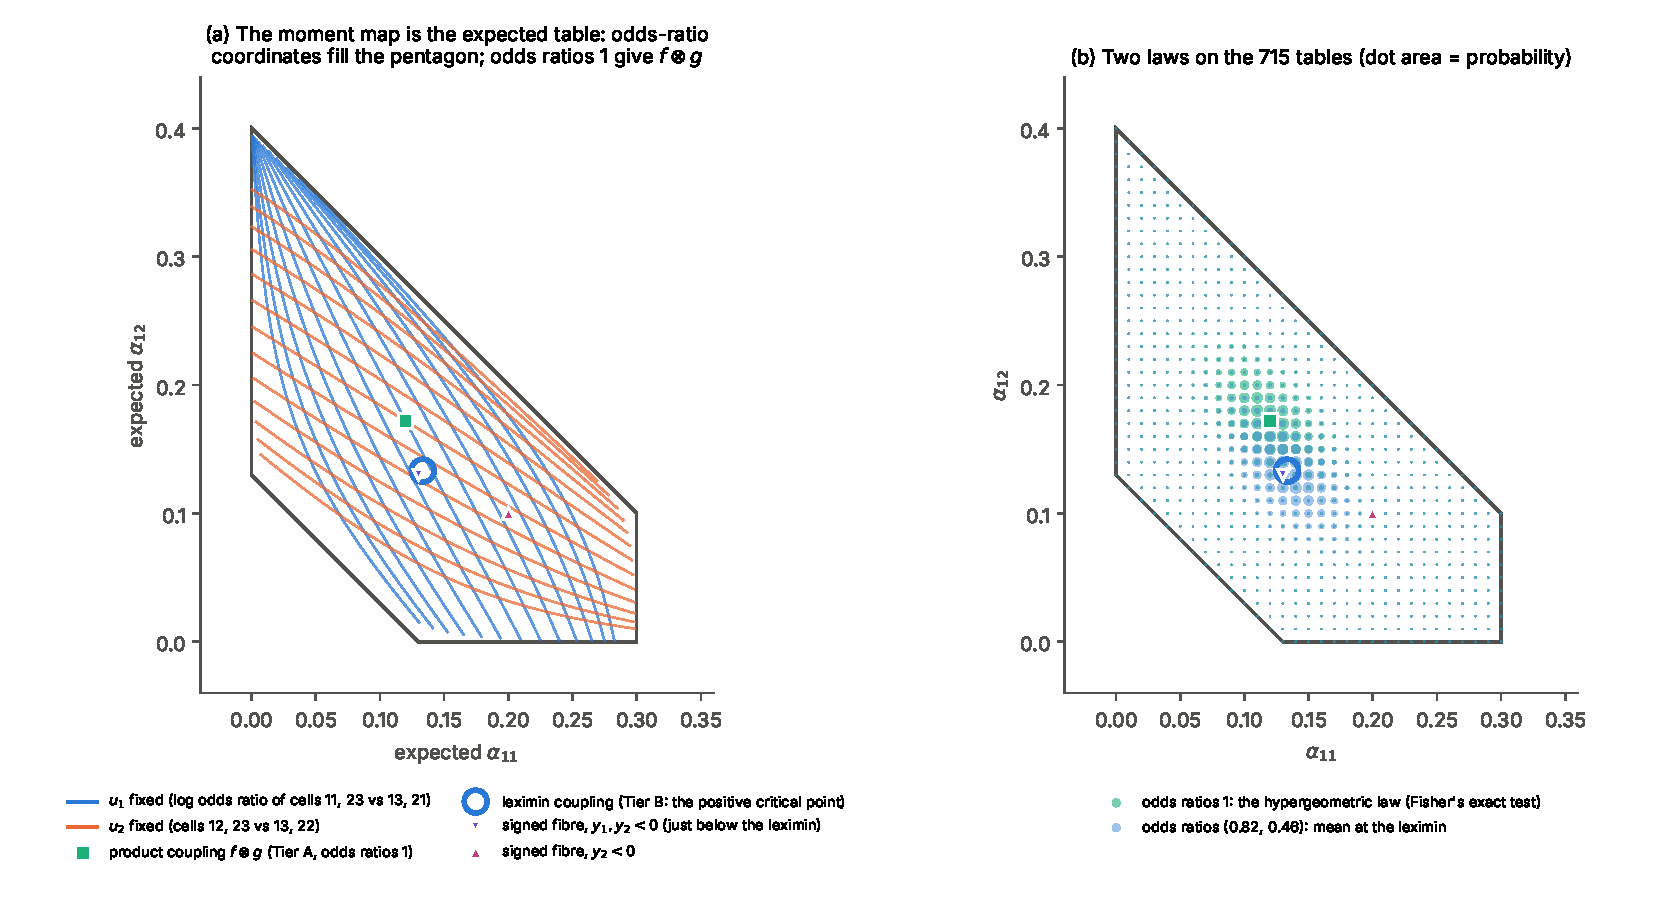
\includegraphics[width=\linewidth]{fig_cpl_tierA.pdf}
\caption{Tier~A. (a) The moment map sends the plane of log odds ratios onto the open pentagon. Blue lines hold $u_1$ fixed and orange lines hold $u_2$ fixed. (b) Two
laws on the $715$ tables: the hypergeometric law (odds ratios $1$, centred on $f\otimes g$), and the law with odds ratios $(0.82,0.46)$, centred on the leximin coupling.}\label{fig:cpltierA}
\end{figure}

\subsection{Tier B: the selected coupling is the leximin one}
\begin{theorem}[the max--min coupling]\label{thm:maxmincoupling}
Let $(f,g)$ be nondegenerate $n\times m$ margins, and let $W$ be the potential of $\mathrm{Cpl}(f,g)$, a sum over its facet cells.
\begin{enumerate}
\item[(1)] $h^*=\max_\alpha\min_{c\text{ facet}}\alpha_c=\min\bigl(\min_if_i/m,\ \min_jg_j/n\bigr)$.
\item[(2)] Every cell of a \emph{binding} row or column, one attaining the minimum, is a facet. If exactly one line binds, the leading set $K_0$ is that line's cells.
\item[(3)] The candidate set has dimension $(n-2)(m-1)$ for a binding row and $(n-1)(m-2)$ for a binding column. For $2\times3$, a binding row gives a single candidate, so
  leading order selects. A binding column gives a segment, and the next level selects.
\item[(4)] The positive critical point of $W$ sits over the facet-leximin coupling, the lexicographic max--min of the facet cells. This is \cref{cor:leximin}, which
  follows from the selection theorem (\cref{thm:selection}).
\end{enumerate}
\end{theorem}

\begin{proof}
(1) A row of $m$ cells sums to $f_i$, so its smallest cell is at most $f_i/m$; columns are the same. Conversely, put $h$ (the claimed value) in every cell and add the product of the
residual margins $f_i-mh\ge0$ and $g_j-nh\ge0$, whose totals agree. This gives a coupling with every cell at least $h$. (2) A cell with $\alpha_c>0$ on all of $\mathrm{Cpl}$ has $f_i+g_j>1$. For a
binding row $i$ that would give $f_i>\sum_{k\ne j}g_k\ge(m-1)\min_kg_k$ and $f_i\le(m/n)\min_kg_k$, so $n(m-1)<m$, which is impossible. If row $i$ alone binds, the residual margins of the
other rows and of all columns are positive, so the coupling of (1) has every other cell strictly above $h^*$. The row's cells, which average $h^*$, equal it at every
maximiser. (3) The $m$ cell functionals of a row sum to the constant $f_i$, so their normals span $m-1$ dimensions and contain $0$ in the relative interior of their hull. Apply
\cref{prop:balancelp}(2) in dimension $(n-1)(m-1)$. (4) See \cref{cor:leximin}. CF6 checks it on $20$ random rational margins at $T=10^{-60}$.
CF4 checks (1)--(3) on about $1000$ random margins of shapes $2\times3$, $3\times3$, $2\times4$ and $3\times4$, against the facet-only programme.
\end{proof}

In words: \emph{the selected coupling spreads the scarcest row or column evenly over its cells.} In the example, row~1 binds with $f_1/3=2/15$. So $h^*=2/15$, $K_0=\{11,12,13\}$, and the positive
critical point sits over the leximin coupling $(2/15,2/15)$. The product coupling $f\otimes g=(0.12,0.172)$ has the single leading cell $13$, at $0.108<h^*$, so it is not a candidate. That is
the Tier-B reason why ``the product coupling carries no brane'' \cite{Awasthi2026Br}.

\begin{example}[the five critical points]\label{ex:fivecrit}
$W=y_1+y_2+T^{2/5}/(y_1y_2)+T^{3/10}/y_1+T^{-13/100}y_1y_2$ has $5$ critical points, twice the area $5/2$ of its Newton polygon (Kushnirenko). Exact resultants at $T=10^{-100}$ and $10^{-200}$ place them as follows.
\begin{itemize}[itemsep=1pt]
\item Three lie over the leximin coupling, one of them positive.
\item One is real with $y_1,y_2<0$, over $(13/100,13/100)$. Its leading cells are $\{11,12,23\}$, whose normals have the signed balance $(1,0)+(0,1)-(1,1)=0$ but no positive one.
\item One is real with $y_2<0$, over $(1/5,1/10)$. Its leading cells are $\{12,13,21\}$, also with a signed balance only.
\end{itemize}
This is \cref{thm:bridge}(4) on the example. By the cited theorem \cite{ChoOh2006}, three torus fibres have non-vanishing Floer cohomology. This agrees with \cite[Thm.~8.2]{Awasthi2026Br}. CF5 checks
the count, the positions, the signs and the leading sets.
\end{example}

\subsection{The positive thimble on couplings}
By \cref{thm:tropical}, the positive thimble with $\hbar=T^h$, read in $u=\log y/\log T$, tends to the uniform law on $Q_h=\{\alpha:\text{every facet cell}\ge h\}$ for $h<h^*$, and concentrates on $\operatorname{argmax}$ at $h^*$.
On the fibre this has a plain reading. At $h=0$ it is the uniform law on all couplings, which is Duistermaat--Heckman, and the limit of the uniform law on tables. As $h$
grows it is uniform on the couplings whose every cell is at least $h$. At $h^*=2/15$ it is the leximin coupling (\cref{fig:cplthimble}; CF7). The thimble is thus a one-parameter family of
probability laws on couplings, from ``all equally likely'' to ``the fairest one''.

\begin{figure}[!htbp]\centering
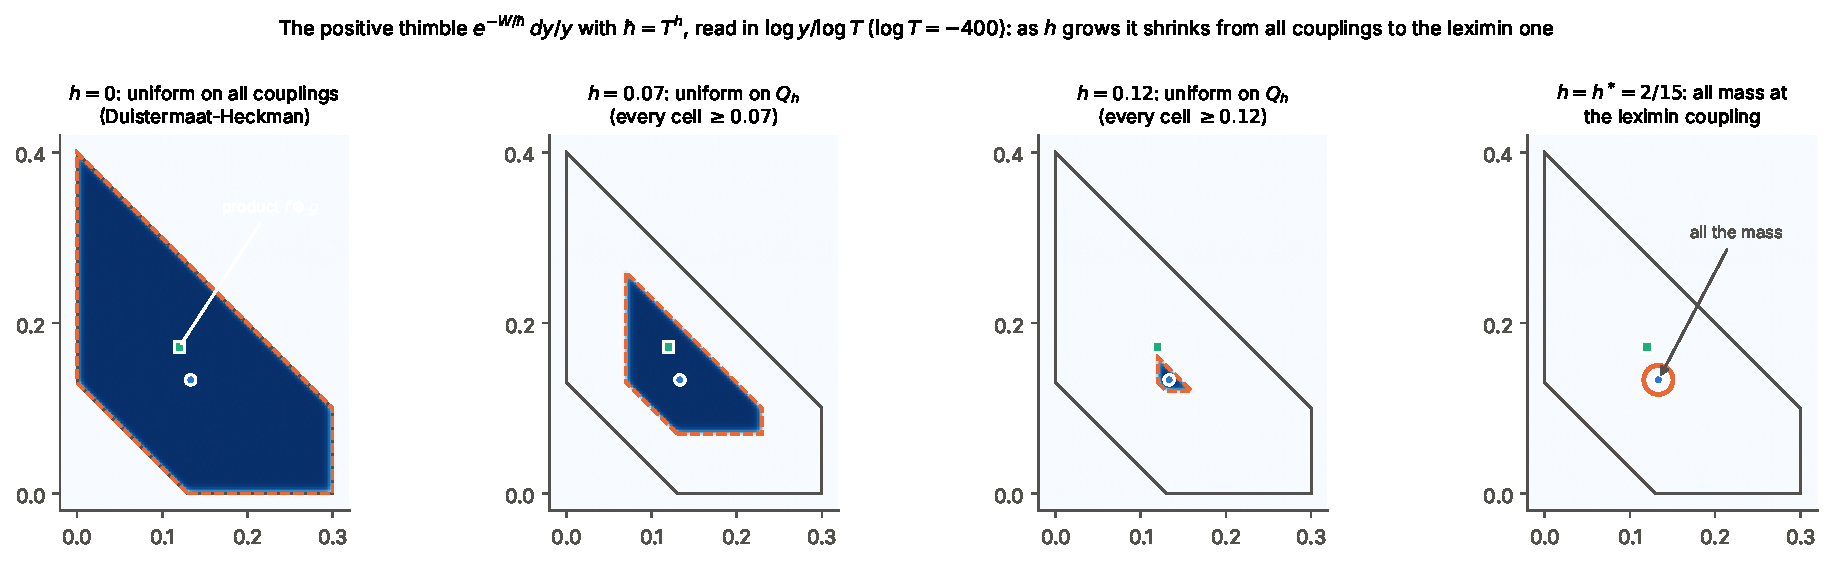
\includegraphics[width=\linewidth]{fig_cpl_thimble.pdf}
\caption{The positive thimble on the fibre, at four values of $h$, with $\log T=-400$. Dashed: the shrunk polygon $Q_h$, every cell at least $h$. The law is uniform on $Q_h$, and at
$h^*=2/15$ all its mass is at the leximin coupling (circle). The product coupling (square) is passed over.}\label{fig:cplthimble}
\end{figure}

\subsection{Two kinds of wall, and one count of data}
In the base, the margins $(f,g)$ move the K\"ahler class of the fibre. Two families of walls cut the base.
\begin{itemize}
\item \emph{K\"ahler-chamber walls} $f(I)=g(J)$. Across them the polygon gains or loses a side, which is a toric blow-up or blow-down \cite{Awasthi2026Cpl}. These are the viability walls of the ledger.
\item \emph{Leximin walls}, where two of the ratios $f_i/m$, $g_j/n$ tie. Across them the binding line, and with it the leading cells and the candidate dimension, jumps
  (\cref{thm:maxmincoupling}). These are the outcome walls of \cref{cor:where}, here explicit.
\end{itemize}
They are different walls (\cref{fig:cplwalls}(a)). The monotone point, with uniform margins, lies on all of them.

\begin{example}[one count]\label{ex:onecount}
In the example, $f_1/3=2/15$ and $g_3/2=27/200$ differ by only $1/600$. Move one observation of $100$ from column~3 to column~2, so that $g=(30,44,26)/100$. Then:
\begin{itemize}[itemsep=1pt]
\item column~3 binds, $h^*=13/100$, and the leading cells are $\{13,23\}$;
\item the candidates become a segment, and the leximin coupling, selected at the next level, is $(27/200,27/200)$;
\item the real critical point with $y_1,y_2<0$ moves onto the leximin fibre, so the distinct valuations drop from three to two. By the cited theorem, so does the number of
  torus fibres with non-vanishing Floer cohomology.
\end{itemize}
The surface does not change: the nearest blow-up wall, $f_1=g_2$, is three counts away. So in this example the least data that changes the perspective is one
count, and it changes the leading cells and the Floer fibres, not the manifold (\cref{fig:cplwalls}(b); CF8, with exact resultants at $T=10^{-100}$ and $10^{-300}$).
\end{example}

\begin{figure}[!htbp]\centering
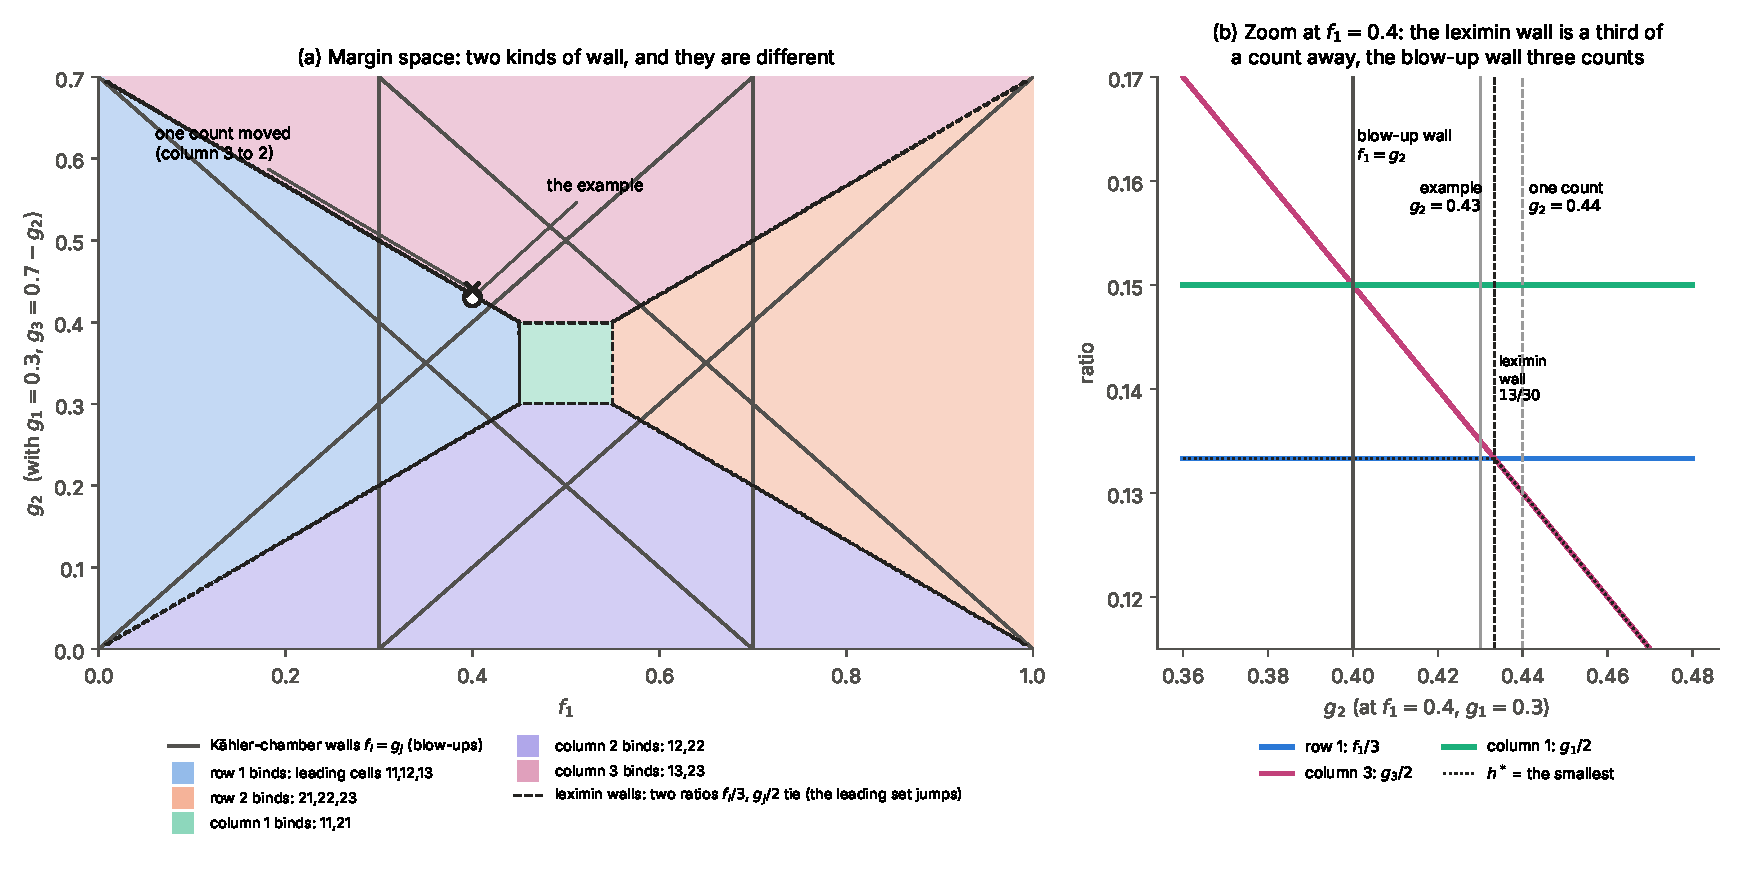
\includegraphics[width=\linewidth]{fig_cpl_walls.pdf}
\caption{Margin space, in the slice $g_1=0.3$. (a) Colours show which row or column binds. Dashed lines are the leximin walls and solid lines the blow-up walls $f_i=g_j$. The
example (circle) sits almost on a leximin wall, and one count (cross) crosses it. (b) Along $f_1=0.4$: the three ratios $f_1/3$, $g_3/2$, $g_1/2$, whose minimum is $h^*$. The leximin wall is a
third of a count from the example, while the blow-up wall $f_1=g_2$ is three counts away.}\label{fig:cplwalls}
\end{figure}

\subsection{The selection theorem, and a column-binding example}\label{sec:selection}
\Cref{thm:bridge} and \cref{prop:balancelp} put the valuation of the positive critical point in the candidate set. When that set is a point, this is the whole answer.
When it is not, as for a binding column, the next level selects. This subsection proves that the levels continue all the way down, for any
configuration.

\begin{definition}[lexicographic max--min]\label{def:lex}
Let $\ell_k(u)=\langle v_k,u\rangle-\lambda_k$ with $v_1,\dots,v_m$ positively spanning $\R^n$. Put $A_0=\R^n$ and $S_0=\emptyset$. For $j\ge1$, let $h_j$ be the maximum over $A_{j-1}$ of the least $\ell_k$ with $k$ not yet
fixed. Let $A_j$ be the set where it is attained, and let $S_j$ be the not-yet-fixed $k$ with $\ell_k\equiv h_j$ on $A_j$. Stop when every $k$ is fixed. Then $A_J$ is a single point, the
\emph{lexicographic max--min point} $u^{\mathrm{lex}}$.
\end{definition}

Each $S_j$ is nonempty (\cref{prop:balancelp}(2), applied on $A_{j-1}$), and each $A_j$ is bounded, so the recursion stops. The fixed normals span $\R^n$, so $A_J$ is a point. On $\mathbb{CP}^2$ and on $F_1$
with $\alpha<1/3$ there is one level. On $F_1$ with $\alpha>1/3$ there are two, as in \cref{ex:levels}.

\begin{theorem}[selection]\label{thm:selection}
Let $a_k(L)\in[c,C]\subset(0,\infty)$, and let $u_L$ minimise $F_L(u)=\sum_ka_k(L)e^{-L\ell_k(u)}$. Then $|u_L-u^{\mathrm{lex}}|=O(1/L)$ as $L\to\infty$. In particular, the valuation of the positive critical
point of $W_T$, with $L=\log(1/T)$ and $u_L=\log y_T/\log T$, is the lexicographic max--min point of the facet functions, and the error at finite $T$ is $O(1/\log(1/T))$.
\end{theorem}

\begin{proof}
$F_L$ is strictly convex and coercive, because the $v_k$ positively span, so $u_L$ is unique. We argue by induction on $n$; the case $n=0$ is empty.

\emph{Level one is pinned to $O(1/L)$.} For $\bar u\in A_1$, $F_L(u_L)\le F_L(\bar u)\le mCe^{-Lh_1}$. So each term satisfies $ce^{-L\ell_k(u_L)}\le mCe^{-Lh_1}$, that is, $\ell_k(u_L)\ge h_1-\kappa/L$ with $\kappa=\log(mC/c)$. By
\cref{prop:balancelp}(2) there is a balanced law $q$ supported exactly on $S_1$, and then $\sum_{k\in S_1}q_k\ell_k\equiv h_1$. Hence $\ell_k(u_L)\le h_1+\kappa/(Lq_{\min})$ for $k\in S_1$.

\emph{The first level drops out.} Let $D_1=\{d:\langle v_k,d\rangle=0,\ k\in S_1\}$ be the direction space of $E_1=\operatorname{aff}A_1$, and $P$ the orthogonal projection onto $D_1$. Then $Pv_k=0$ for $k\in S_1$. So
projecting $\nabla F_L(u_L)=0$ gives, exactly,
\[
\sum_{k\notin S_1}a_k(L)\,e^{-L\ell_k(u_L)}\,Pv_k=0 .
\]
Write $u_L=p_L+w_L$, with $p_L\in E_1$ and $w_L\perp D_1$. The $v_k$, $k\in S_1$, span $D_1^\perp$, and $\langle v_k,w_L\rangle=\ell_k(u_L)-h_1=O(1/L)$, so $|w_L|=O(1/L)$. Hence $p_L$ is a critical point, and so the
minimiser, of $F^{(1)}_L(p)=\sum_{k\notin S_1}a'_k(L)e^{-L\ell_k(p)}$ on $E_1$. Here $a'_k=a_ke^{-L\langle v_k,w_L\rangle}$ again lies in a fixed compact subset of $(0,\infty)$.

\emph{Induction.} On $E_1$ the remaining $\ell_k$ have projected normals $Pv_k$ that positively span $D_1$, because $A_1=\{p\in E_1:\ell_k(p)\ge h_1,\ k\notin S_1\}$ is bounded. Their lexicographic max--min
point is $u^{\mathrm{lex}}$. Indeed, off $A_1$ some remaining $\ell_k$ is below $h_1$, while on the relative interior of $A_1$ all exceed it, so the reduced recursion is levels $2,3,\dots$ of the original.
Since $\dim D_1<n$, the induction hypothesis gives $|p_L-u^{\mathrm{lex}}|=O(1/L)$, and so $|u_L-u^{\mathrm{lex}}|=O(1/L)$.
LX1--LX3 corroborate the statement and the mechanism, on $30$ random configurations in multiprecision arithmetic.
\end{proof}

\begin{remark}[provenance]
The procedure is the one Fukaya, Oh, Ohta and Ono use to locate a non-displaceable fibre \cite{FOOO2010}. Judd and Rietsch construct the tropical critical point
recursively, and prove that it maximises the tropicalisation \cite{JuddRietsch2019}. A related hierarchical selection governs the exponential-penalty trajectory in linear
programming \cite{CominettiSanMartin1994}. The statement is therefore adapted; the proof above is direct, and it gives the rate. The constant in $O(1/L)$ depends on the gaps between levels. That is
why the near tie of \cref{ex:onecount} converged slowly.
\end{remark}

\begin{corollary}[the selected coupling]\label{cor:leximin}
For nondegenerate $n\times m$ margins, the positive critical point of the potential of $\mathrm{Cpl}(f,g)$ sits over the facet-leximin coupling. In $292$ random margins of shapes
$2\times3$, $3\times3$ and $2\times4$, this equals the leximin coupling over all cells (LX4). We have not proved that the two always agree.
\end{corollary}

\begin{example}[a column-binding fibre]\label{ex:colbind}
Repurpose Example~3.4(b) of \cite{Awasthi2026Cpl}: $f=(2/5,3/5)$, $g=(1/2,3/10,1/5)$. The fibre is the pentagon with vertices $(1/5,0)$, $(2/5,0)$, $(1/10,3/10)$, $(0,3/10)$, $(0,1/5)$ and area $11/200$. Its facets are the
cells $11,12,13,22,23$. Cell $21$ never vanishes, since $f_2+g_1=11/10$. The ratios are $f_i/3=(2/15,1/5)$ and $g_j/2=(1/4,3/20,1/10)$, so column~3 binds. The levels are:
\begin{center}\small
\begin{tabular}{lll>{\raggedright\arraybackslash}p{0.5\linewidth}}\toprule
level & value & cells fixed & what is decided\\\midrule
1 & $h_1=1/10$ & $13,23$ & column~3 is spread evenly; the candidates form the open segment $x+y=3/10$, $1/10<x<1/5$\\
2 & $h_2=3/20$ & $11,12,22$ & along the segment, the least remaining cell is largest at the midpoint\\\bottomrule
\end{tabular}
\end{center}
So $u^*=(3/20,3/20)$ (\cref{fig:leximin}(a),(b)). The endpoints are maximisers but not candidates: their leading sets, $\{11,13,22,23\}$ and $\{12,13,23\}$, have no positive balance. At finite $T$,
\[
x_L=\tfrac{3}{20}+\frac{\ln2}{2L}+o(1/L),
\]
because cells $11$ and $22$ coincide on the segment (both equal $x$) and balance cell $12$ alone: $2e^{-Lx}=e^{-L(3/10-x)}$ (\cref{fig:leximin}(c)). Of the five critical points, the positive one
and a real one with $y_1,y_2<0$ sit over $(3/20,3/20)$, both with this correction. The other three (one real, two complex) lie over the fibre $(2/15,1/6)$ on the candidate segment, off the leximin point. \Cref{sec:cbclass} derives this exactly. The slow approach seen at finite $T$ is
the $1/\log(1/T)$ effect of their leading moduli $2^{\pm1/3}$. The positive thimble shows the two levels as $h$ grows: it is uniform on the segment at
$h=1/10$, uniform on $[h,3/10-h]$ between the levels, and concentrated at $3/20$ above (\cref{fig:leximin}(d)). The one-count example of \cref{ex:onecount} is column-binding too, with levels
$(13/100;\,13,23)$ and $(27/200;\,11,12)$. LX5--LX9 check every number here, the first exactly.
\end{example}

\begin{figure}[!htbp]\centering
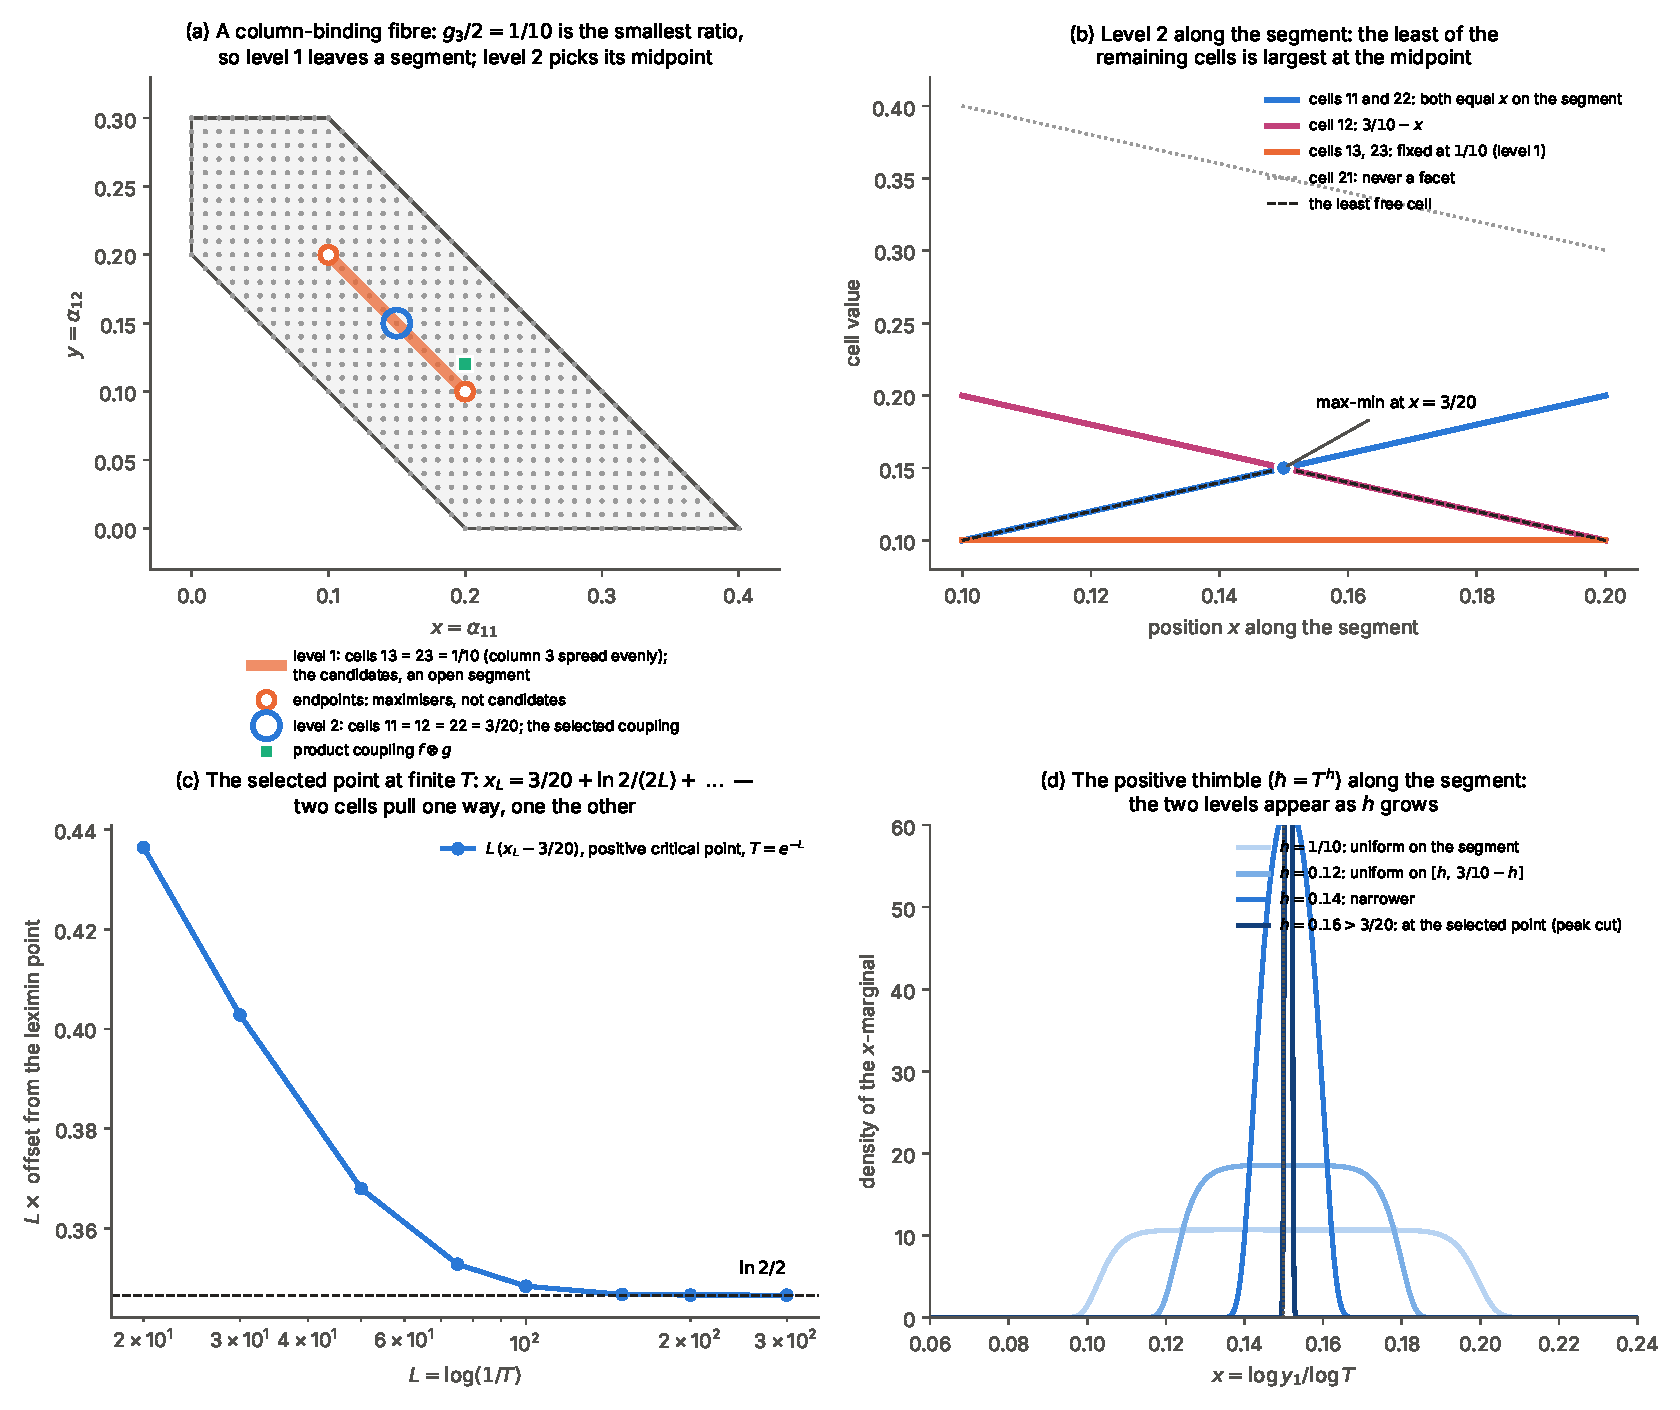
\includegraphics[width=\linewidth]{fig_leximin.pdf}
\caption{The selection theorem on a column-binding fibre. (a) Level~1 fixes cells $13$ and $23$ at $1/10$ and leaves a segment of candidates, whose endpoints are not candidates.
Level~2 picks its midpoint. (b) Along the segment, the least remaining cell is largest at $x=3/20$. (c) At finite $T$ the selected point is offset by $\ln2/(2L)$, because two cells pull
against one. (d) The positive thimble along the segment shows both levels as $h$ grows.}\label{fig:leximin}
\end{figure}

\subsection{The example through every layer}

\begin{center}\small
\begin{tabular}{>{\raggedright\arraybackslash}p{0.17\linewidth}>{\raggedright\arraybackslash}p{0.58\linewidth}>{\raggedright\arraybackslash}p{0.17\linewidth}}\toprule
layer & in the example & where\\\midrule
fibre & pentagon, area $1331/20000$, facets $11,12,13,21,23$; $715$ tables (Pick) & \cref{ex:pentagon}; CF1--2\\
Tier A & Fisher's noncentral hypergeometric family; odds ratios $1$ give $f\otimes g=(0.12,0.172)$; the leximin needs $(0.82,0.46)$ & \cref{prop:hypergeom}; CF3\\
Tier B & $h^*=f_1/3=2/15$; row~1 binds; one candidate, the leximin coupling $(2/15,2/15)$ & \cref{thm:maxmincoupling}; CF4, CF6\\
selection & the valuation is the lexicographic max--min point, error $O(1/\log(1/T))$; a binding column needs a second level & \cref{thm:selection,ex:colbind}; LX1--LX9\\
sign split & five critical points; signed fibres over $(13/100,13/100)$ and $(1/5,1/10)$ & \cref{ex:fivecrit}; CF5\\
Floer (cited) & three fibres with non-vanishing Floer cohomology; none over $f\otimes g$ & \cite{ChoOh2006,Awasthi2026Br}\\
thimble & uniform on couplings at $h=0$; uniform on $Q_h$; the leximin coupling at $h^*$ & \cref{thm:tropical}; CF7\\
walls & leximin wall $1/600$ away in ratio; blow-up wall $f_1=g_2$ three counts away & \cref{fig:cplwalls}\\
one count & column~3 binds; candidates a segment; three Floer fibres become two; same surface & \cref{ex:onecount}; CF8\\
not claimed & other thimbles, Stokes data, stability conditions, the category & \cref{sec:outlook}\\\bottomrule
\end{tabular}
\end{center}

\part{Towards morphisms}
\section{Objects, morphisms and a categorical comparison}\label{sec:morph}
\begin{center}\colorbox{stAdapted!60}{\begin{minipage}{0.94\linewidth}\small
\textbf{What this section shows, in plain words.} So far we have found \emph{which} torus fibres matter. A category also needs the arrows between them.
\begin{itemize}[leftmargin=1.4em,itemsep=1pt]
\item Every critical point of $W$ is an \emph{object}: a torus fibre with a local system. Distinct objects have no arrows between them, and each object's arrows to itself
  form a Clifford algebra. For the probabilistic object, its quadratic form is the Fisher information of the conditioned law (\cref{fig:morphobjects}).
\item Up to equivalence, an outcome wall does \emph{not} change the category. It moves objects between fibres.
\item It does leave two traces. The Clifford form of the probabilistic object, reduced modulo $T$, drops rank exactly when the candidate set stops being a point (\cref{fig:morphclifford}).
  And the Stokes walls, where the basis of thimbles mutates, crowd into a window of width $O(1/\log(1/T))$ around the outcome wall (\cref{fig:morphstokes}).
\end{itemize}
The computations are all on the critical points, values and Hessians of $W$. The Floer reading of those data is cited, and its status is marked in each statement.
\end{minipage}}\end{center}

\subsection{Objects}
By \cite{ChoOh2006}, a critical point $c$ of $W$ with valuation $u_c$ gives the torus fibre $L(u_c)$ with a rank-one local system. Its holonomy has leading term $y_c/T^{u_c}$, and $L(u_c)$ has
non-vanishing Floer cohomology. We call the pair an \emph{object}. In our examples $W$ has $\chi(X)$ critical points, twice the area of its Newton polygon: $4$ for $F_1$ and $5$ for $\mathrm{Bl}_2\mathbb{CP}^2$.
\begin{center}\small
\begin{tabular}{>{\raggedright\arraybackslash}p{0.24\linewidth}>{\raggedright\arraybackslash}p{0.7\linewidth}}\toprule
example & objects: fibre, type, leading holonomy\\\midrule
$F_1$, $\alpha=1/5$ & over the barycentre: positive $(1,1)$, complex $(\zeta,\zeta)$, $(\zeta^2,\zeta^2)$, with $\zeta^3=1$; over $(1/5,3/5)$: real-signed $(-1,1)$\\
$F_1$, $\alpha=3/5$ & all four over $(2/5,1/5)$: positive $(1,1)$, real-signed $(-1,1)$, complex $(i,-1)$, $(-i,-1)$\\
$2\times3$ example & over the leximin coupling $(2/15,2/15)$: positive and two complex; over $(13/100,13/100)$: real $(-1,-1)$; over $(1/5,1/10)$: real $(1,-1)$\\
one count later & over $(27/200,27/200)$: positive, real $(-1,-1)$, two complex; over $(1/5,1/10)$: real $(1,-1)$\\\bottomrule
\end{tabular}
\end{center}
MO1 and MO2 check this table, the first part from the quartic and the second from exact resultants at $T=10^{-200}$.

\begin{figure}[!htbp]\centering
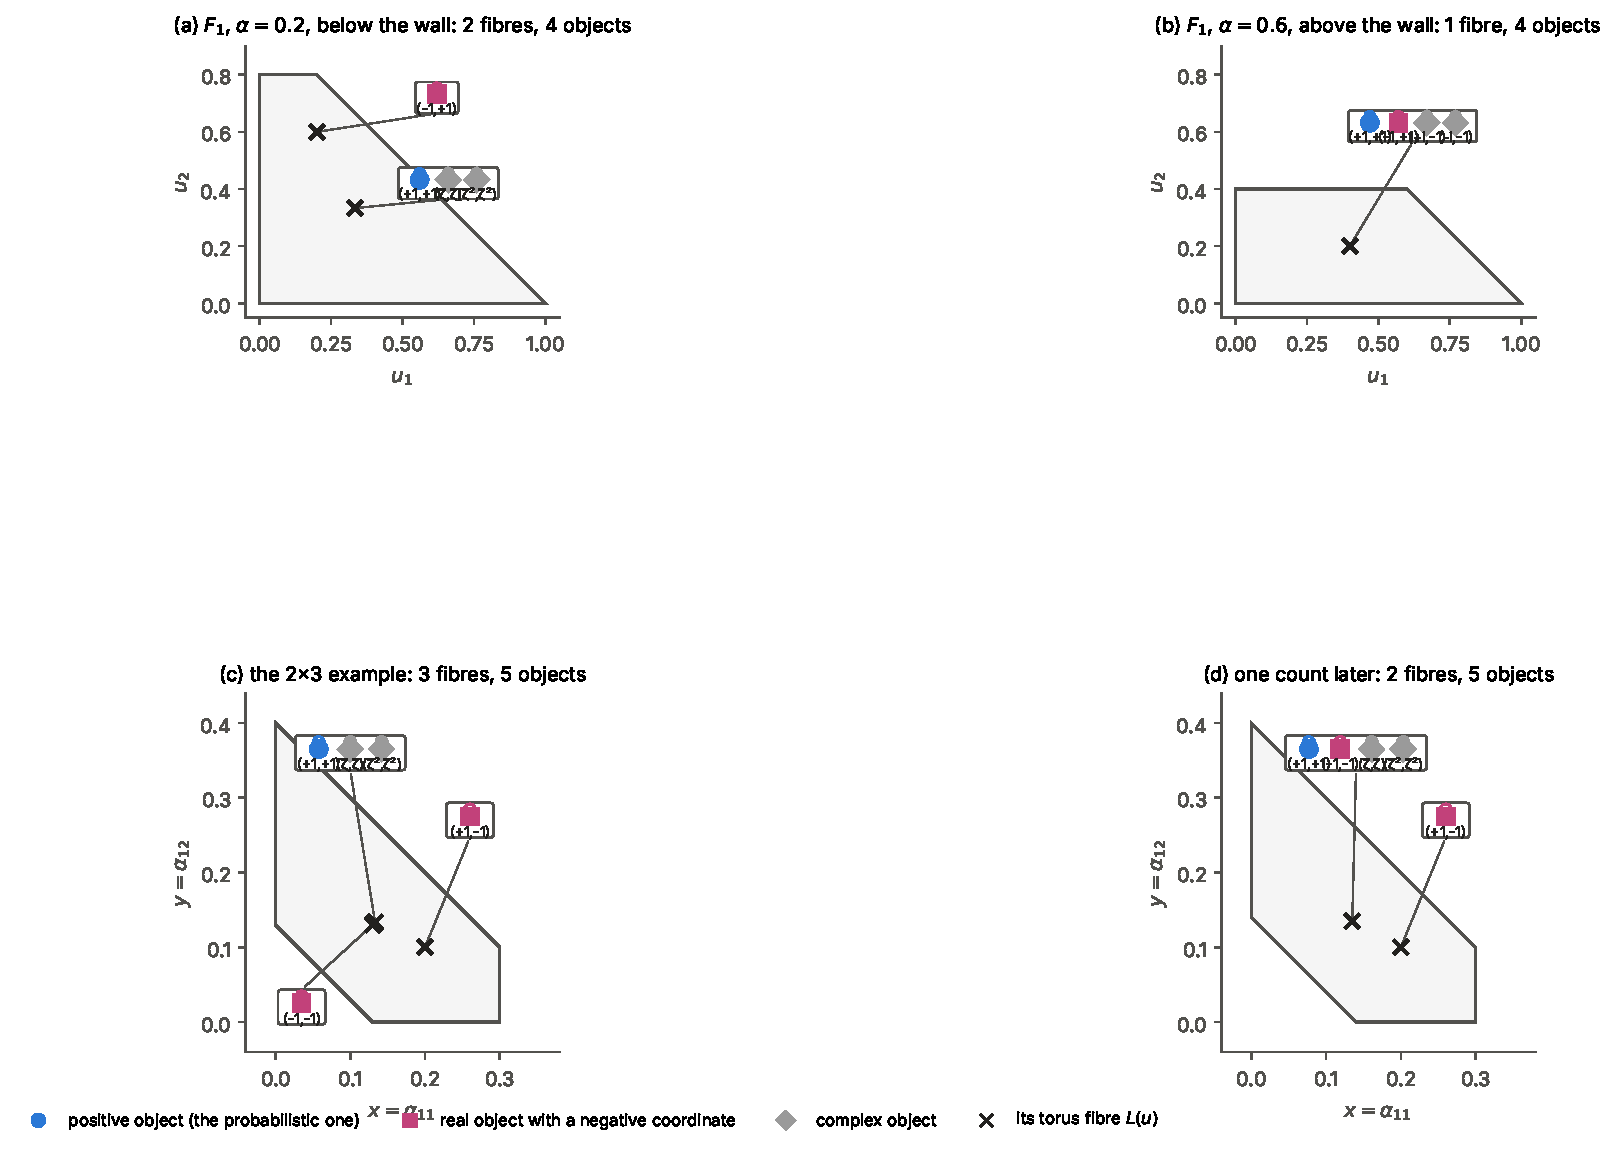
\includegraphics[width=0.92\linewidth]{fig_morph_objects.pdf}
\caption{Objects over their torus fibres (crosses). Each box is a fibre; each marker is an object, labelled by its leading holonomy; each loop is its endomorphism
algebra $\mathrm{Cl}_2$. There are no arrows between distinct objects. (a)$\to$(b): crossing the $F_1$ wall merges two fibres into one. (c)$\to$(d): one count of data merges the
leximin fibre with the nearby real fibre. In both cases the objects persist; only their fibres change.}\label{fig:morphobjects}
\end{figure}

\subsection{Morphisms}
\begin{proposition}[morphisms between the objects]\label{prop:morph}
\begin{enumerate}
\item[(1)] Objects over distinct fibres have no morphisms: distinct moment fibres are disjoint, so their Floer complex is zero (exact).
\item[(2)] Distinct objects over one fibre have distinct critical values $W(c)=m_0$. Morphisms are defined only between objects with equal $m_0$, so the category splits into summands $\mathcal F_\lambda$
  \cite{Auroux2007,FOOO2010}, and they have no morphisms. This uses distinct $m_0$ only. Their holonomies also differ, but we do not use that to separate objects: an
  eigenvalue decomposition cannot by itself separate two objects with the same $m_0$. That these objects generate their summands is proved in the monotone case and conditionally otherwise \cite{Smith2018}; our examples are not monotone.
\item[(3)] The Floer cohomology ring of an object is the Clifford algebra of the Hessian $Q=\sum_kc_kv_kv_k^{\!\top}$ of $W$ at $c$, where $c_k$ are the values of its terms \cite[Thm.~5.6]{Cho2005}.
  So it has dimension $2^n$.
\item[(4)] For the positive object, $Q=W\cdot\operatorname{Cov}_w(v)$, where $w$ is the law of the terms of $W$ at $y_T$ (mean exponent $0$). Its quadratic form is the Fisher information of the conditioned law,
  scaled by $W$. It is real and positive definite.
\end{enumerate}
\end{proposition}

\begin{proof}
(1) $L(u)=\mu^{-1}(u)$. (2) and (3) are the cited theorems; MO3 checks that the critical values (and, for the record, the holonomies) are distinct in every example. (4) $Q=\sum_kc_kv_kv_k^{\!\top}$ with $c_k=Ww_k$,
and $\sum_kw_kv_k=0$. MO4 and MO5 check the identity, and the Clifford relations with explicit generators that span $M_2$, for all $18$ objects.
\end{proof}

\subsection{The \texorpdfstring{$A_\infty$}{A-infinity} products}
\begin{proposition}[no higher products survive]\label{prop:formal}
Over the algebraically closed Novikov field $\Lambda$, let $Q$ be nondegenerate. The $\mathbb Z/2$-graded algebra $\mathrm{Cl}(Q)$ is separable. For $n=2$ it is the super matrix algebra $\mathrm{End}(\Lambda^{1|1})$. Its
Hochschild cohomology vanishes in positive degrees. So every $A_\infty$ structure on it, with $m_1=0$ and this $m_2$, is $A_\infty$-isomorphic to the formal one: it is intrinsically formal
\cite{Kadeishvili1980,SeidelThomas2001}. On the subcategory generated by these objects, the higher products $m_k$ for $k\ge3$ can be removed by an $A_\infty$ isomorphism.
\end{proposition}

\begin{proof}
A separable algebra has vanishing Hochschild cohomology in positive degrees. The obstructions to formality lie in $HH^{k,2-k}$ for $k\ge3$, so they vanish. MO5 exhibits
$\mathrm{Cl}(Q)\cong M_2$ for every object. The statement rests on the cited $m_2$ of \cref{prop:morph}(3); we do not compute the $A$-side higher products themselves.
\end{proof}

So, within what the cited theorems give, the category generated by the objects is $\bigoplus_c\mathrm{Cl}(Q_c)$. It is semisimple, with one summand per critical point, matching $\dim QH^*(X)=\chi(X)$. On the
mirror side, matrix factorisations at a nondegenerate critical point have the same Clifford description \cite{Dyckerhoff2011}.

\subsection{The Clifford shadow of selection}
Over $\Lambda$, all Clifford algebras of nondegenerate forms of rank $n$ are isomorphic, so (2)--(3) cannot see an outcome wall. The integral form can.

\begin{theorem}[the Clifford shadow]\label{thm:shadow}
Write the Clifford form of the positive object in the integral basis of $H^1(L;\mathbb Z)$ and divide it by $W$. Then $Q/W=\operatorname{Cov}_w(v)$ has entries of non-negative valuation. Its reduction modulo
$T$ is $\operatorname{Cov}_{q^*}(v)$, where $q^*$ is the limit law of \cref{thm:bridge}(2). Its rank is $\dim\sigma_0=n-\dim(\text{candidate set})$. So the reduced Clifford algebra is semisimple exactly when the
candidate set is a single point, that is, exactly when leading order selects.
\end{theorem}

\begin{proof}
$w_k$ has valuation $\ell_k(u^*)-h^*\ge0$, and $w\to q^*$ by \cref{thm:bridge}(2). $\operatorname{Cov}_{q^*}(v)=\sum_kq^*_kv_kv_k^{\!\top}$, because $q^*$ has mean $0$. Its rank is the dimension of the span of $\{v_k:k\in K_0\}$, which is $\dim\sigma_0$
because $0\in\operatorname{relint}\sigma_0$. Then apply \cref{prop:balancelp}(2). MO6 checks the convergence and the ranks.
\end{proof}

In the examples, the other eigenvalues have valuation equal to the gap between selection levels. On $F_1$ above the wall the small eigenvalue is $\sim T^{(3\alpha-1)/4}$, where
$(3\alpha-1)/4=h_2-h_1$; it closes at the wall (\cref{fig:morphclifford}(a)). On the $2\times3$ fibre, one count turns rank $2$ into rank $1$, with valuation $1/200=h_2-h_1$ (\cref{fig:morphclifford}(b)). In the
column-binding example the valuation is $1/20$. So the hierarchy of selection reappears as the hierarchy of scales of the probabilistic object's Clifford form.

\begin{figure}[!htbp]\centering
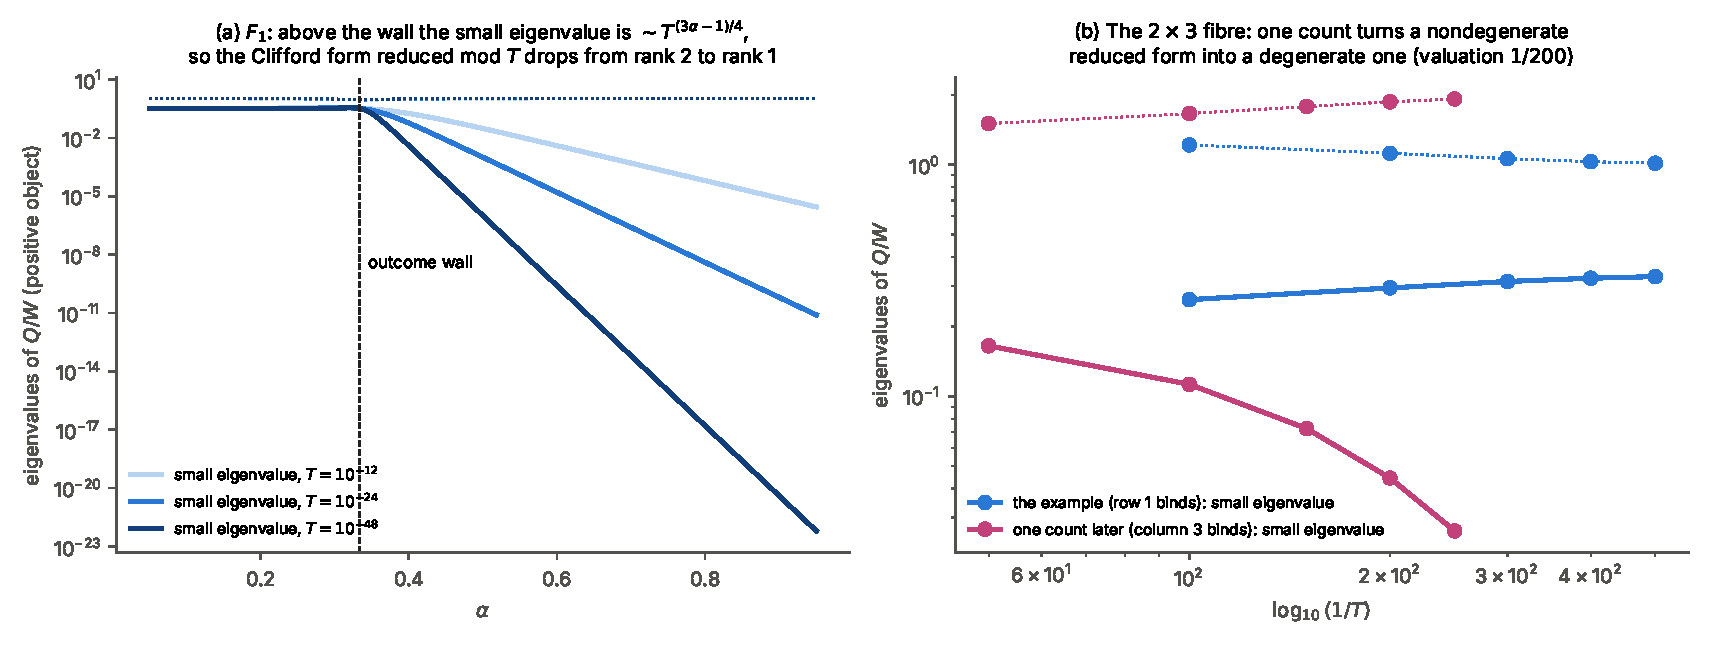
\includegraphics[width=\linewidth]{fig_morph_clifford.pdf}
\caption{The Clifford shadow. (a) $F_1$: eigenvalues of $Q/W$ for the positive object (solid: the small one; dotted: the large one) at three values of $T$. Above the wall the small
eigenvalue tends to $0$ like $T^{(3\alpha-1)/4}$, so the form reduced mod $T$ has rank $1$. (b) The $2\times3$ fibre, before and after one count. After the move the small eigenvalue decays like
$T^{1/200}$.}\label{fig:morphclifford}
\end{figure}

\subsection{Comparing the two sides of a wall}
Three mechanisms could relate the two sides of a wall: an $A_\infty$ functor, a continuation map, or a mutation. Here is what each does.

\begin{theorem}[an $A_\infty$ equivalence across the $F_1$ wall]\label{thm:compare}
On $F_1$, for every $T\in(0,1)$ and every $\alpha\in(0,1)$, the four critical points are distinct and nondegenerate. So they form four continuous branches in $\alpha$, and the semisimple
categories $\bigoplus_c\mathrm{Cl}(Q_c(\alpha))$ over $\Lambda$ are related by algebra isomorphisms that depend continuously on $\alpha$. For the positive object these are real: $A^{\!\top}Q(\alpha')A=Q(\alpha)$. In
particular they are $A_\infty$ equivalences across $\alpha=1/3$. What changes at the wall is the \emph{support}: which fibre carries which object. That is the merging of fibres in \cref{fig:morphobjects}.
\end{theorem}

\begin{proof}
The discriminant $-27T^2-256T^{3-3\alpha}$ never vanishes (\cref{ex:F1wall}(d)), so the critical points never collide, and nondegeneracy follows. A nondegenerate complex symmetric form has a
symmetric square root, which gives the isomorphisms. MO7 checks the path $\alpha\in[1/5,3/5]$ at $T=10^{-24}$. The $A$-side reading is that of \cref{prop:morph,prop:formal}, so the statement inherits
their status.
\end{proof}

\emph{Continuation maps} compare Floer theory of Hamiltonian-isotopic Lagrangians in one symplectic manifold. Here the evidence moves the K\"ahler class itself, and distinct fibres are
not Hamiltonian isotopic. So there is no continuation map in the strict sense: the family comparison of \cref{thm:compare} takes its place.

\emph{Mutations} belong to the category of thimbles, the Fukaya--Seidel category of the Landau--Ginzburg model. For a phase $\theta$ of $\hbar$, a distinguished basis of thimbles changes by a
mutation when two critical values align along $\theta$ \cite{Seidel2008}.

\begin{proposition}[Stokes walls crowd the outcome wall]\label{prop:stokes}
On $F_1$, the Stokes walls for the phases $\theta=0.3$, $1$ and $\pi/2$ lie within $4/\log(1/T)$ of $\alpha=1/3$, for $T=10^{-12},10^{-24},10^{-48}$, and $\log(1/T)\,(\alpha_\theta-1/3)$ does not depend on $T$.
Away from the window there are none. The mechanism is that $|W|$ is $\sim T^{\alpha}$ for the signed object and $\sim T^{1/3}$ for the barycentre objects. Outside a window of width $O(1/\log(1/T))$ one of them dominates, and
the phases of the differences are frozen; inside it their ratio sweeps $(0,\infty)$, and every phase is crossed. For real $\hbar$ ($\theta=0$) the positive thimble never mutates: it is the positive
orthant for every $\lambda$ (\cref{prop:thimble}).
\end{proposition}

This is a computation, MO8 and MO9, with the mechanism sketched; we have not proved the window for general configurations.

\begin{figure}[!htbp]\centering
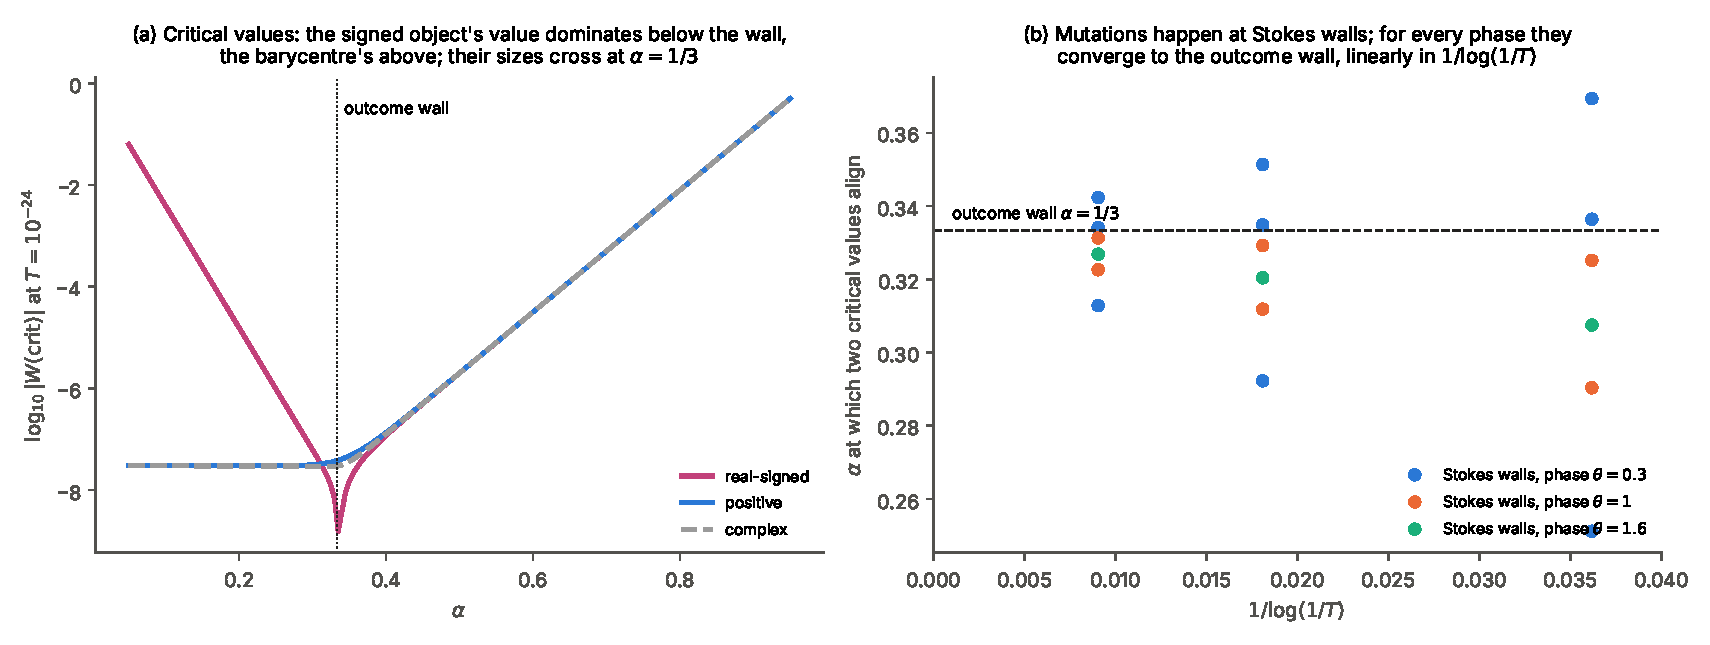
\includegraphics[width=\linewidth]{fig_morph_stokes.pdf}
\caption{Mutations and the outcome wall on $F_1$. (a) The sizes of the four critical values at $T=10^{-24}$: the signed object's value dominates below the wall, and the barycentre objects'
values above it. (b) The Stokes walls for three phases, at three values of $T$, lie on lines through $(0,1/3)$ in the variable $1/\log(1/T)$.}\label{fig:morphstokes}
\end{figure}

\subsection{What sees the wall}
\begin{center}\small
\begin{tabular}{>{\raggedright\arraybackslash}p{0.38\linewidth}>{\raggedright\arraybackslash}p{0.28\linewidth}>{\raggedright\arraybackslash}p{0.24\linewidth}}\toprule
invariant & across the outcome wall & status\\\midrule
which fibres carry objects & changes ($2\to1$; $3\to2$) & cited \cite{ChoOh2006}; MO1--2\\
the category over $\Lambda$, $\bigoplus\mathrm{Cl}(Q_c)$ & unchanged, up to $A_\infty$ equivalence & \cref{thm:compare}, on cited $m_2$\\
higher products & none survive & \cref{prop:formal}, on cited $m_2$\\
the positive object's Clifford form mod $T$ & rank drops ($2\to1$) & \cref{thm:shadow}, new\\
the thimble basis at phase $\theta\ne0$ & mutates within $O(1/\log(1/T))$ of the wall & \cref{prop:stokes}, computed\\
the positive thimble, real $\hbar$ & never changes & \cref{prop:thimble}, proved\\\bottomrule
\end{tabular}
\end{center}
So a data-induced outcome wall is not a wall of the Fukaya category over $\Lambda$. It is a wall of its \emph{integral} structure for the probabilistic object, and the place where, at finite $T$,
the thimble bases mutate. The full $A_\infty$ category over $\Lambda_0$, and split generation in the non-monotone case, are left open.

\subsection{The column-binding example, classified}\label{sec:cbclass}
The column-binding fibre of \cref{ex:colbind} is the first example whose objects are not all over the selected fibre, and whose holonomies are not all of modulus one. Stage IV (\cref{sec:path}) shows why: the example lies on a level-two leximin wall, and both features belong to the wall. We classify
its five critical points exactly, then compute the morphisms between the resulting objects. Wall-crossing from this example is deferred.

\paragraph{The Floer convention.} We use the convention of \cite{FOOO2010}. An object is a pair $(L(u),b)$ with $b\in H^1(L(u);\Lambda_0)$, whose holonomy coordinates are $y_i=T^{u_i}e^{b_i}$. Their
leading coefficients $e^{b_{i,0}}$ are arbitrary nonzero complex numbers, not only those of modulus one, so local systems with non-unit leading modulus are included. On a compact toric
Fano manifold the potential is $W$ \cite{ChoOh2006}. The pair has non-vanishing Floer cohomology iff $y$ is a critical point of $W$, and $m_0(L(u),b)=W(y)\cdot1$ \cite{FOOO2010}. For the Clifford
description of the endomorphism ring we use the formula $Q=\operatorname{Hess}W$ at $y$ \cite[Thm.~5.6]{Cho2005}. Cho states it in the setting of \cite{ChoOh2006}, and its use with non-unit leading
coefficients is the one place where our citation goes beyond the original setting.

With $\tau=T^{1/10}$, the potential of this fibre is $W=y_1+y_2+\tau^4/(y_1y_2)+\tau^3/y_2+y_1y_2/\tau^2$ (cells $11,12,13,22,23$).

\begin{proposition}[the five critical points]\label{prop:five}
\begin{enumerate}
\item[(1)] \emph{Reduction.} $y_1\partial_1W-y_2\partial_2W=y_1-y_2+\tau^3/y_2$. So $y_1=s-\tau^3/s$ with $s=y_2$, and the remaining equation is exactly
\[
q(s)=s^5+\tau^2s^4-2\tau^3s^3-2\tau^5s^2+\tau^8=0 .
\]
  Since $q(0)\ne0$ and $q$ has no common root with $s^2-\tau^3$, the critical points correspond one to one to the roots of $q$.
\item[(2)] \emph{Newton polygon.} The lower hull of $q$ has vertices $(0,8)$, $(3,3)$, $(5,0)$. The edge of slope $-5/3$, with edge polynomial $1-2c^3$, gives three roots $s\approx2^{-1/3}\omega\,\tau^{5/3}$ with $\omega^3=1$. The
  edge of slope $-3/2$, with edge polynomial $c^2-2$, gives two roots $s\approx\pm\sqrt2\,\tau^{3/2}$.
\item[(3)] \emph{Distinct and nondegenerate for every $T>0$.} $\operatorname{disc}_sq=-\tau^{31}(256\tau^2-837\tau+3456)$, and the resultant of $q$ with the Hessian determinant is $\tau^{54}(256\tau^2-837\tau+3456)$. The quadratic has
  discriminant $-2838375<0$, so neither vanishes for $\tau>0$.
\item[(4)] \emph{Distinct critical values for every $T\in(0,1)$.} $W=2s+\tau^4/(s^2-\tau^3)+(s^2-\tau^3)/\tau^2$ at a critical point. The polynomial whose roots are the five critical values has discriminant
  $-\tau^{225}(\tau-1)^2(256\tau^2-837\tau+3456)^3$, which vanishes on $(0,\infty)$ only at $T=1$.
\end{enumerate}
\end{proposition}

\begin{proof}
Each statement is an exact symbolic computation (CB1--CB4). In (2) the edge polynomials are read off the coefficients on each edge: $\tau^8-2\tau^3s^3$ and $-2\tau^3s^3+s^5$.
\end{proof}

So there are five critical points, two fibres and five objects:
\begin{center}\small
\begin{tabular}{>{\raggedright\arraybackslash}p{0.15\linewidth}>{\raggedright\arraybackslash}p{0.11\linewidth}>{\raggedright\arraybackslash}p{0.22\linewidth}>{\raggedright\arraybackslash}p{0.21\linewidth}>{\raggedright\arraybackslash}p{0.15\linewidth}}\toprule
object & fibre & leading $(y_1,y_2)/T^{u}$ & leading $W$ & leading $\det(Q/W)$\\\midrule
$P$ positive & $(\tfrac3{20},\tfrac3{20})$ & $(\tfrac{\sqrt2}2,\ \sqrt2)$ & $2\tau+2\sqrt2\,\tau^{3/2}$ & $\sqrt2\,\tau^{1/2}$\\
$N$ real $(-,-)$ & $(\tfrac3{20},\tfrac3{20})$ & $(-\tfrac{\sqrt2}2,\ -\sqrt2)$ & $2\tau-2\sqrt2\,\tau^{3/2}$ & $-\sqrt2\,\tau^{1/2}$\\
$R$ real $(-,+)$ & $(\tfrac2{15},\tfrac16)$ & $(-2^{1/3},\ 2^{-1/3})$ & $-2\tau+2^{2/3}\tau^{5/3}$ & $-c\,\tau^{2/3}$\\
$C_\omega$, $C_{\bar\omega}$ complex & $(\tfrac2{15},\tfrac16)$ & $(-2^{1/3}\bar\omega,\ 2^{-1/3}\omega)$ & $-2\tau+2^{2/3}\omega\,\tau^{5/3}$ & $-c\,\bar\omega^2\tau^{2/3}$\\\bottomrule
\end{tabular}
\end{center}
Here $c=3\cdot2^{-4/3}$, $\omega=e^{\pm2\pi i/3}$, and $C_{\bar\omega}$ is the conjugate of $C_\omega$. CB5 and CB6 check every entry against the roots at $\tau=10^{-10},10^{-20},10^{-40}$, with relative errors $1.5\cdot10^{-4}$, $6.8\cdot10^{-8}$ and
$1.5\cdot10^{-14}$. The two groups have opposite leading critical value, $\pm2\tau$. Within a group the values separate at order $\tau^{3/2}$, or at order $\tau^{5/3}$ through the cube roots of unity (\cref{fig:cbnewton}).

\begin{figure}[!htbp]\centering
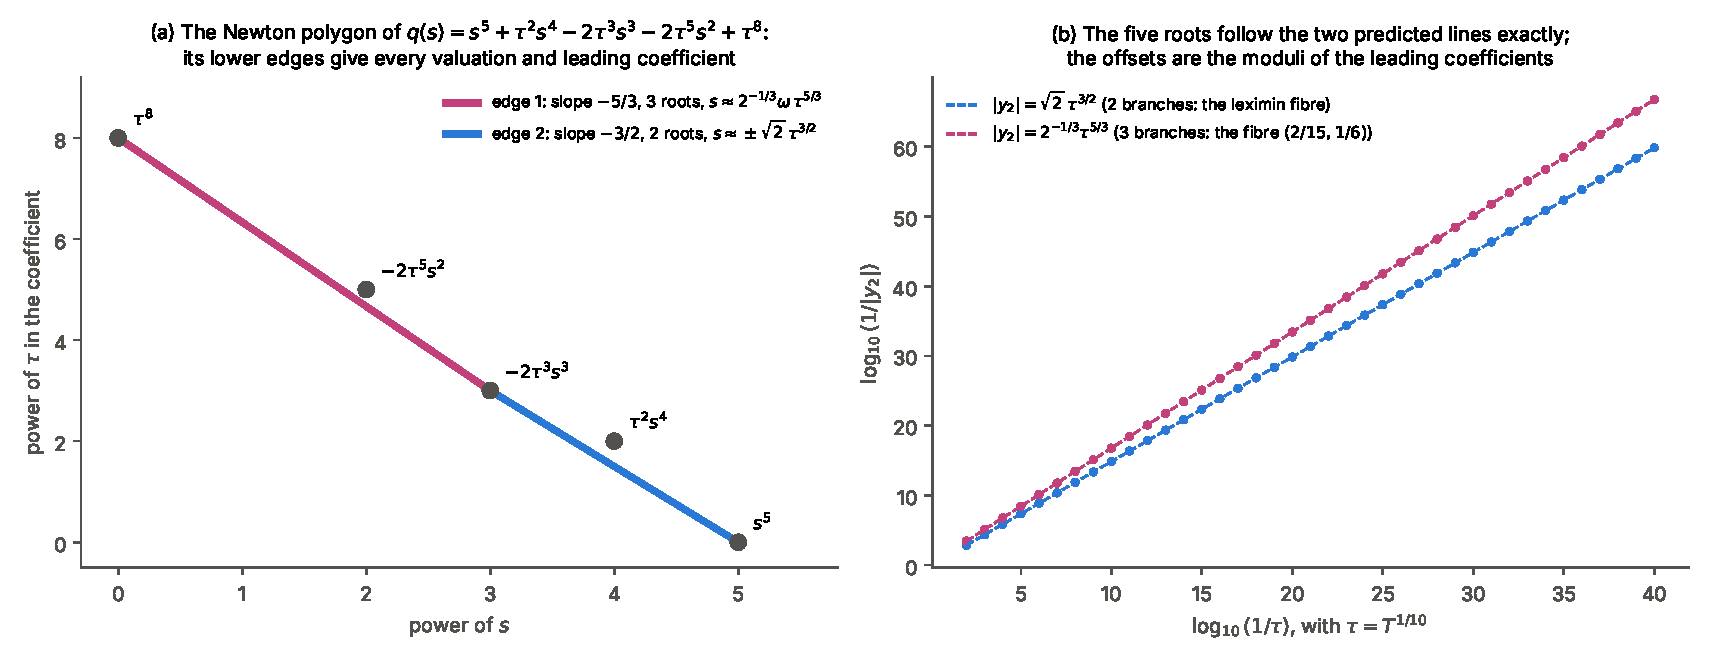
\includegraphics[width=\linewidth]{fig_cb_newton.pdf}
\caption{The column-binding example classified. (a) The Newton polygon of the quintic: one edge gives the three branches over $(2/15,1/6)$, the other the two over the leximin fibre. (b) The five
roots against $\tau$ follow the two predicted lines; the vertical offsets are the moduli of the leading coefficients.}\label{fig:cbnewton}
\end{figure}

\begin{remark}[the drift explained]
At finite $T$ a branch with leading coefficient $\rho$ has apparent valuation $u-\log|\rho|/\log(1/T)$. For $P$, $\log(\sqrt2/2)$ gives the offset $\ln2/(2L)$ of \cref{ex:colbind}. For the other three, $\log2^{\pm1/3}$ gives
$\pm\ln2/(3L)$. This was the slow ``drift'' seen there: the limits are exactly $(2/15,1/6)$. The three sit there because their level-one terms have $y_1y_2\approx-\tau^3$. This sign makes the level-two terms
(cells $11$ and $22$) cancel exactly, so the position is set by the next balance, of cell $12$ against the constant term: $-2\tau^3s^3+\tau^8\approx0$. In the row-binding examples every leading coefficient
has modulus one. Non-unit moduli appear here because a level of selection cancels.
\end{remark}

\begin{theorem}[reduction of the Clifford form]\label{thm:reduction}
Let $c$ be a nondegenerate critical point with valuation $u_c$. Let $K$ be its leading set, the $k$ with $\ell_k(u_c)$ minimal, equal to $h_c$. Write the term values as $c_k=\rho_kT^{h_c}(1+o(1))$ for $k\in K$, and assume
\begin{enumerate}
\item[(H1)] $\sum_{k\in K}\rho_k\ne0$.
\end{enumerate}
Then $Q/W$ has entries of non-negative valuation and reduces modulo $T$ to $M_c=\sum_{K}\rho_kv_kv_k^{\!\top}/\sum_K\rho_k$. Always $\operatorname{rank}M_c\le\dim\operatorname{span}\{v_k:k\in K\}$. Equality holds under
\begin{enumerate}
\item[(H2)] the $\rho_k$, $k\in K$, are real and of one sign,
\end{enumerate}
in particular for the positive object (\cref{thm:shadow}). Without (H2), cancellation can lower the rank.
\end{theorem}

\begin{proof}
By (H1), $W=(\sum_K\rho_k)T^{h_c}(1+o(1))$, and every $c_k$ has valuation at least $h_c$. Under (H2), $\sum_K\rho_kv_kv_k^{\!\top}$ is a semidefinite Gram matrix, whose rank is that of $\{v_k\}$. CB8 tests the theorem on $23$
objects: $F_1$ at $\alpha=1/5$ and $3/5$, the $2\times3$ example, its one-count neighbour, and this example. (H1) holds for all $23$, and (H2) for $13$. The rank equals the span dimension in all $23$, including
the $10$ without (H2). An example is the signed object of $F_1$ at $\alpha=1/5$, where $\rho=(-1,-1,1)$ and $M_c=\left(\begin{smallmatrix}2&1\\1&0\end{smallmatrix}\right)$.
\end{proof}

In the column-binding example $K=\{13,23\}$ for all five objects, with $\rho=(1,1)$ on the leximin fibre and $(-1,-1)$ on the other. (H2) holds, and $M_c=J=\left(\begin{smallmatrix}1&1\\1&1\end{smallmatrix}\right)$, of rank $1$, for every object. The
reduced Clifford algebras are therefore all non-semisimple. The objects are told apart one order further:
\begin{gather*}
P,N:\quad \frac QW=J\pm\frac{\tau^{1/2}}2\operatorname{diag}\!\Bigl(\tfrac{\sqrt2}2,\tfrac{3\sqrt2}2\Bigr)+\dots,\\
R,C:\quad \frac QW=J+2^{-2/3}\bar\omega\,\tau^{1/3}\operatorname{diag}(1,-1)+\dots
\end{gather*}
For $P$ and $N$ the correction is first order in the small direction, so the small eigenvalue is $\pm(\sqrt2/2)\tau^{1/2}$, of valuation $1/20$ in $T$. The form is positive definite for $P$ and indefinite for $N$. For $R$ and $C$ the first-order
correction vanishes in the small direction, which is the cancellation the reduction theorem warns about. The small eigenvalue appears only at second order, $-\tfrac32\,2^{-4/3}\bar\omega^2\tau^{2/3}$, of
valuation $1/15$.

\begin{proposition}[the Hom table]\label{prop:homtable}
In the convention above, the five objects have the following morphisms.
\begin{enumerate}
\item[(1)] Between the two fibres: none. The fibres are disjoint, so the unperturbed Floer complex is zero; this is a legitimate model, since the pair is transverse.
\item[(2)] Within a fibre: none. The critical values are distinct (\cref{prop:five}(4)), and morphisms are defined only between objects with equal $m_0$ \cite{Auroux2007,FOOO2010}. (Their holonomies are also distinct, but the argument does not use this.)
\item[(3)] On the diagonal: $\mathrm{Cl}(Q_c)\cong M_2$, with $Q_c$ as above (cited, in the convention stated). No higher products survive (\cref{prop:formal}).
\end{enumerate}
So the category these objects generate is $\bigoplus_{c=1}^5\mathrm{Cl}(Q_c)$ over $\Lambda$. Over $\Lambda_0$, all five reduce to the rank-one form $J$. Generation of the Fukaya summands remains conditional, because the
example is not monotone \cite{Smith2018}.
\end{proposition}

\begin{proof}
(1) $L(u)=\mu^{-1}(u)$. (2) and (3) are the cited statements together with \cref{prop:five}. CB7 checks the counts, the distinct values and holonomies within each fibre, and that explicit Clifford
generators span $M_2$.
\end{proof}

\begin{figure}[!htbp]\centering
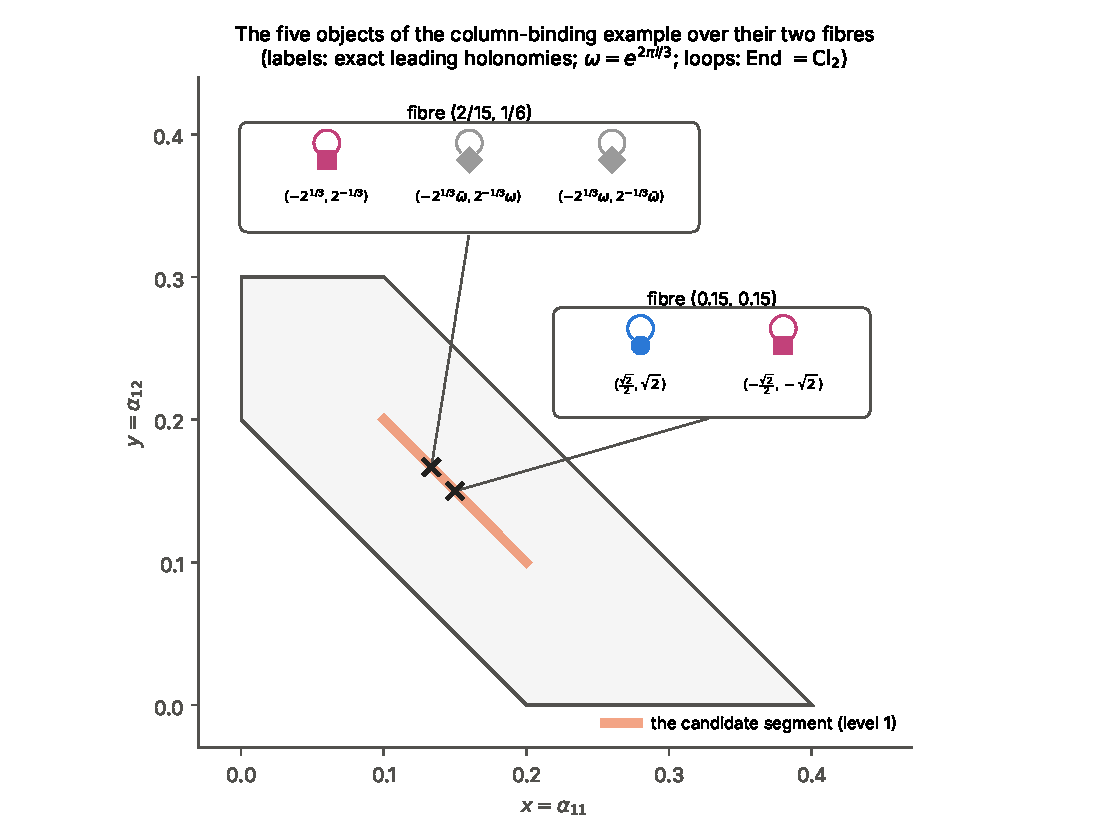
\includegraphics[width=0.66\linewidth]{fig_cb_objects.pdf}\\[4pt]
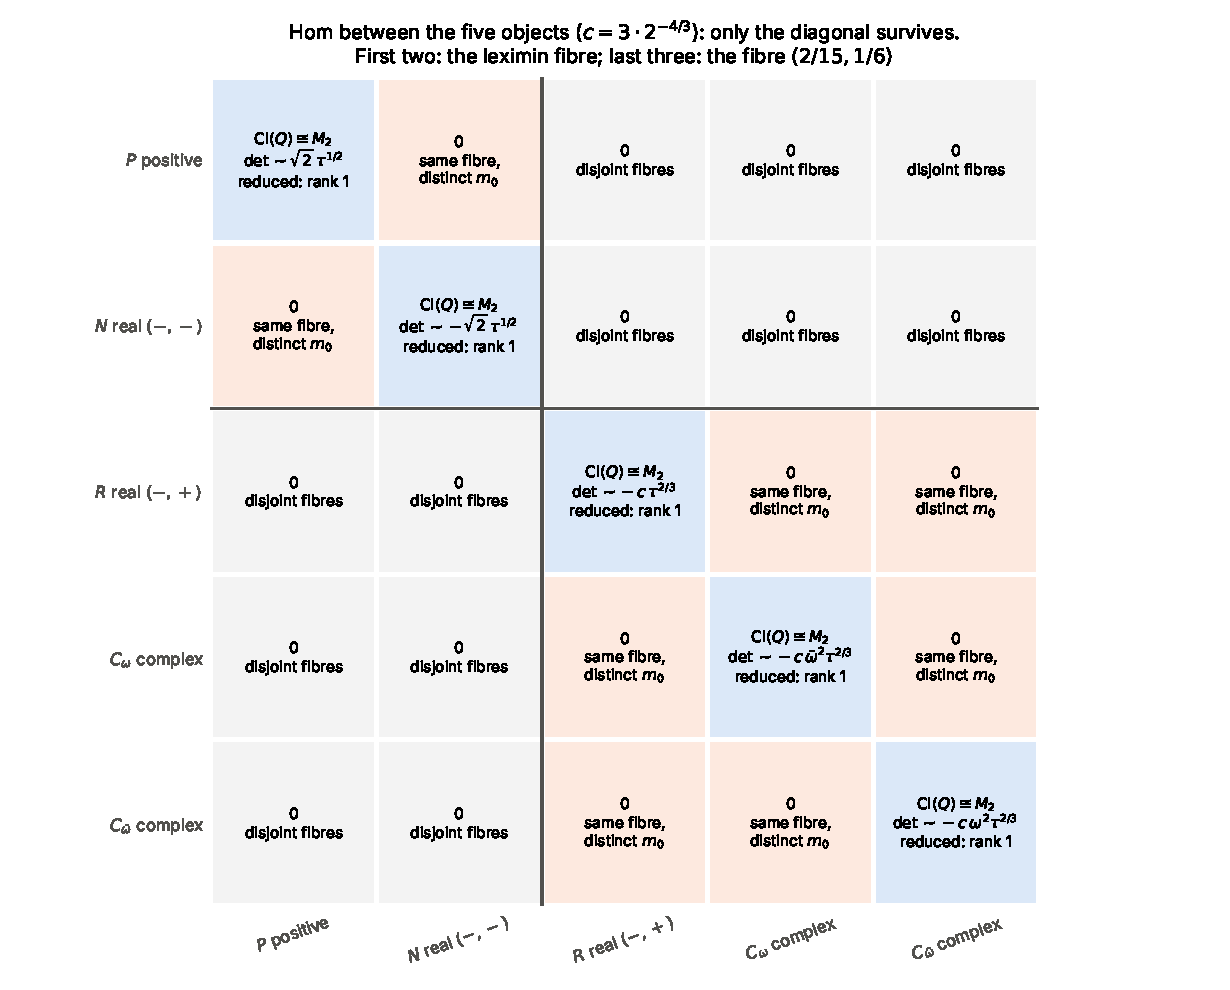
\includegraphics[width=0.66\linewidth]{fig_cb_hom.pdf}
\caption{Top: the five objects over their two fibres, with exact leading holonomies; the leximin fibre carries $P$ and $N$, the fibre $(2/15,1/6)$ carries $R$, $C_\omega$ and $C_{\bar\omega}$. Bottom: the Hom table.
Grey cells vanish because the fibres are disjoint, orange cells because the values of $m_0$ differ. The diagonal is $\mathrm{Cl}(Q_c)\cong M_2$, and every one reduces to the rank-one form $J$ modulo $T$.}\label{fig:cbobjects}
\end{figure}

\subsection{Stage IV: a path through the column-binding example}\label{sec:path}
Data so far moved margins by one count (a point) or along one direction of evidence (a line). Here we take a sheet of margins and one path across it, and we keep four questions separate along the
path: do critical points collide, do critical values coincide, which fibres carry the objects, and what do the Clifford forms and the Stokes alignments see?

\paragraph{The sheet and the path.} Fix $f=(2/5,3/5)$ and let the column margins vary: $g=(1-g_2-g_3,\,g_2,\,g_3)$. \Cref{fig:s4sheet} shows this sheet with its blow-up walls $f_1=g(J)$, which bound the
K\"ahler chambers, and its leximin walls. The path is
\[
g(\gamma)=\Bigl(\tfrac7{10}-\gamma,\ \tfrac3{10},\ \gamma\Bigr),\qquad \gamma\in\bigl[\tfrac3{20},\tfrac{11}{40}\bigr].
\]
It stays in the pentagon chamber (facets $11,12,13,22,23$; no blow-up wall meets $\gamma\in(1/10,3/10)$), and only the exponent of cell $23$ moves. With $A=T^{2/5}$, $B=T^{3/10}$ and $C=T^{\gamma-2/5}$,
\[
W_\gamma=y_1+y_2+\frac{A}{y_1y_2}+\frac{B}{y_2}+C\,y_1y_2 .
\]
The column-binding example of \cref{sec:cbclass} is $\gamma=1/5$.

\begin{figure}[!htbp]\centering
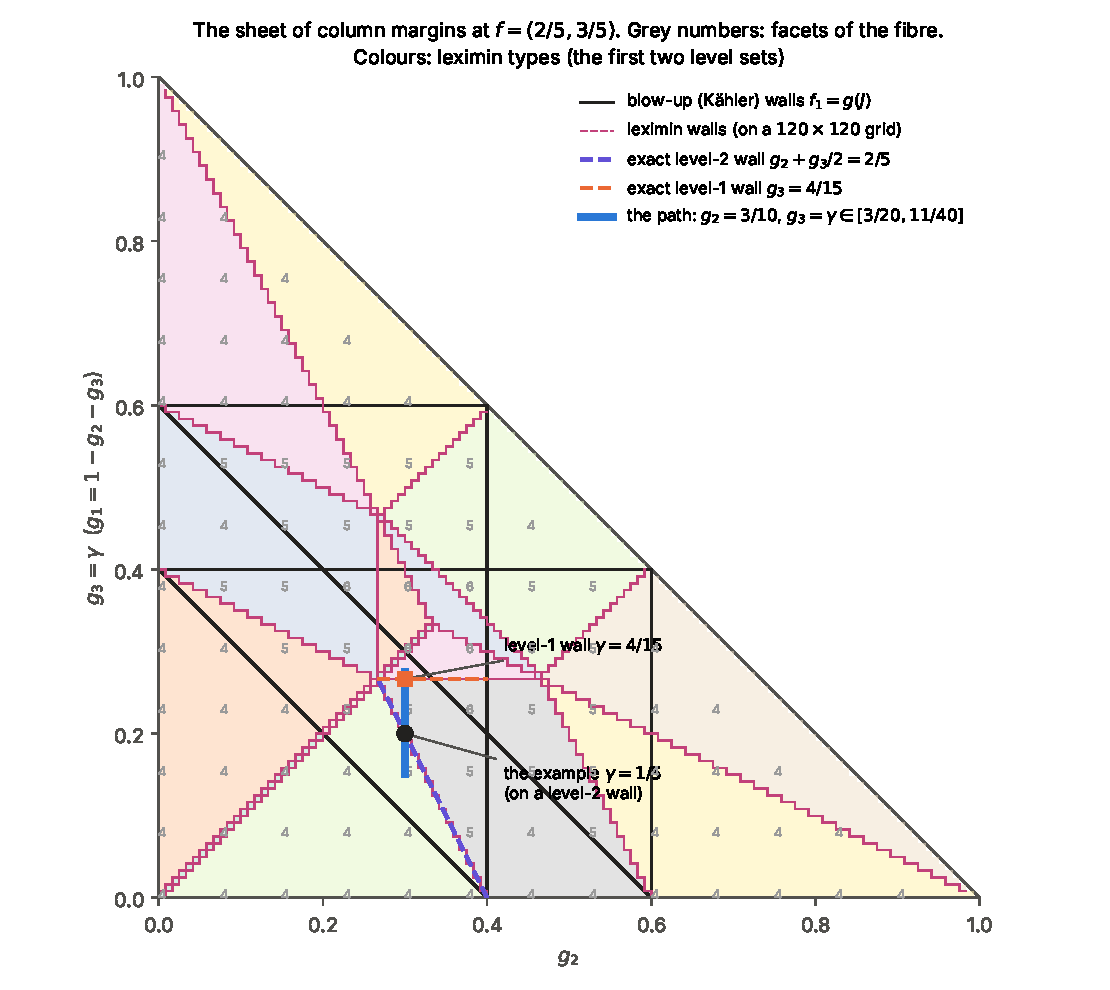
\includegraphics[width=0.7\linewidth]{fig_s4_sheet.pdf}
\caption{The sheet of column margins at $f=(2/5,3/5)$. Black lines are blow-up walls. The stepped rose lines are leximin walls computed on a $120\times120$ grid (colours: leximin types),
and the dashed lines are the two walls the path crosses, drawn exactly: $g_2+g_3/2=2/5$ (level two) and $g_3=4/15$ (level one). Grey numbers count the facets of the fibre. The path (blue) runs inside one K\"ahler chamber, the pentagon, and crosses two leximin walls: the column-binding example (black dot) sits on a level-two wall, and the
level-one wall (orange square) is at $\gamma=4/15$.}\label{fig:s4sheet}
\end{figure}

\begin{proposition}[the path, exactly]\label{prop:path}
\begin{enumerate}
\item[(1)] \emph{Two leximin walls.} For $\gamma<1/5$ the levels are $\gamma/2$ (column $3$), $3/20$ (column $2$) and $1/4-\gamma/2$ (cell $11$). For $1/5<\gamma<4/15$ they are $\gamma/2$ and $(4/5-\gamma)/4$, where
the residual of row $1$ binds. For $\gamma>4/15$ row $1$ binds at once, at $2/15$. At $\gamma=1/5$ the cells $11,12,22$ tie at the second level, and at $\gamma=4/15$ the cells $11,12,13,23$ tie at the first.
So \emph{the column-binding example lies on a level-two leximin wall.}
\item[(2)] \emph{Reduction.} The critical points are $y_1=(s^2-B)/s$, $y_2=s$, where
\begin{equation}\label{eq:pathquintic}
(s^2-B)^2(1+Cs)=As .
\end{equation}
At $\gamma=1/5$, where $C=A/B^2$, this is the quintic of \cref{prop:five}.
\item[(3)] \emph{Where the objects sit.} The Newton polygon of \eqref{eq:pathquintic} changes exactly at the two leximin walls, and gives
\begin{center}\footnotesize\setlength{\tabcolsep}{3pt}
\begin{tabular}{lp{0.47\linewidth}p{0.33\linewidth}}\toprule
$\gamma$ & over the leximin fibre & elsewhere\\\midrule
$(3/20,1/5)$ & $4$, at $(1/4-\gamma/2,\,3/20)$: $s=\pm T^{3/20}$, $y_1=\pm T^{1/4-\gamma/2}$ & $R$, at $(\gamma-1/10,\,2/5-\gamma)$, signs $(+,-)$\\
$1/5$ & $2$, at $(3/20,3/20)$ & $3$, at $(2/15,1/6)$ (\cref{prop:five})\\
$(1/5,4/15)$ & $4$, at $\frac{4/5-\gamma}4(1,1)$: $y_1\approx y_2=i^kT^{(4/5-\gamma)/4}$ & $R$, at $(1/10,1/5)$, signs $(-,+)$\\
$(4/15,11/40]$ & $3$, at $(2/15,2/15)$: $y_1\approx y_2=\omega^kT^{2/15}$ & $N$, at $(2/5-\gamma)(1,1)$, signs $(-,-)$; and $R$\\\bottomrule
\end{tabular}
\end{center}
In every regime the leximin fibre carries the multiple root, as \cref{thm:selection} requires of the positive object.
\end{enumerate}
\end{proposition}

\begin{proof}
(1) By \cref{thm:maxmincoupling} and the recursion of \cref{def:lex}. After column $3$ binds, the segment has $a_{11}+a_{12}=r=2/5-\gamma/2$, and the facet cells on it are $11,12,22$. The residual row binds if
$r<g_2=3/10$, that is, if $\gamma>1/5$, and column $2$ binds otherwise; row $1$ binds at the first level once $\gamma/2>2/15$. (2) As in \cref{prop:five}: $y_1\partial_1W-y_2\partial_2W=y_1-y_2+B/y_2$. (3) Three
dominant balances in \eqref{eq:pathquintic} decide everything. Whether $Cs$ or $1$ dominates on the leximin roots switches at $\gamma=4/15$. Whether $C$ or $A/B^2$ dominates on the isolated root switches at
$\gamma=1/5$. And below $1/5$ the leximin roots have $s^2=B(1+o(1))$: writing $s^2-B=\delta$ gives $\delta^2\approx A/C$, so $y_1=\delta/s$ has valuation $1/4-\gamma/2$. PP2--PP5 check the levels, the Newton
polygons at $10$ rational $\gamma$, and the valuations and phases at $L=200,400$.
\end{proof}

So the peculiarities found in \cref{sec:cbclass} belong to the wall, not to column binding. The grouping $2+3$, the fibre $(2/15,1/6)$ and the leading moduli $2^{\pm1/3}$ occur only at $\gamma=1/5$. On either side
of it, four objects sit over the leximin fibre with leading moduli one. This is what the remark on the drift meant by a level of selection that cancels: there the linear coefficient $B^2C-A$ of
\eqref{eq:pathquintic} vanishes identically.

\begin{figure}[!htbp]\centering
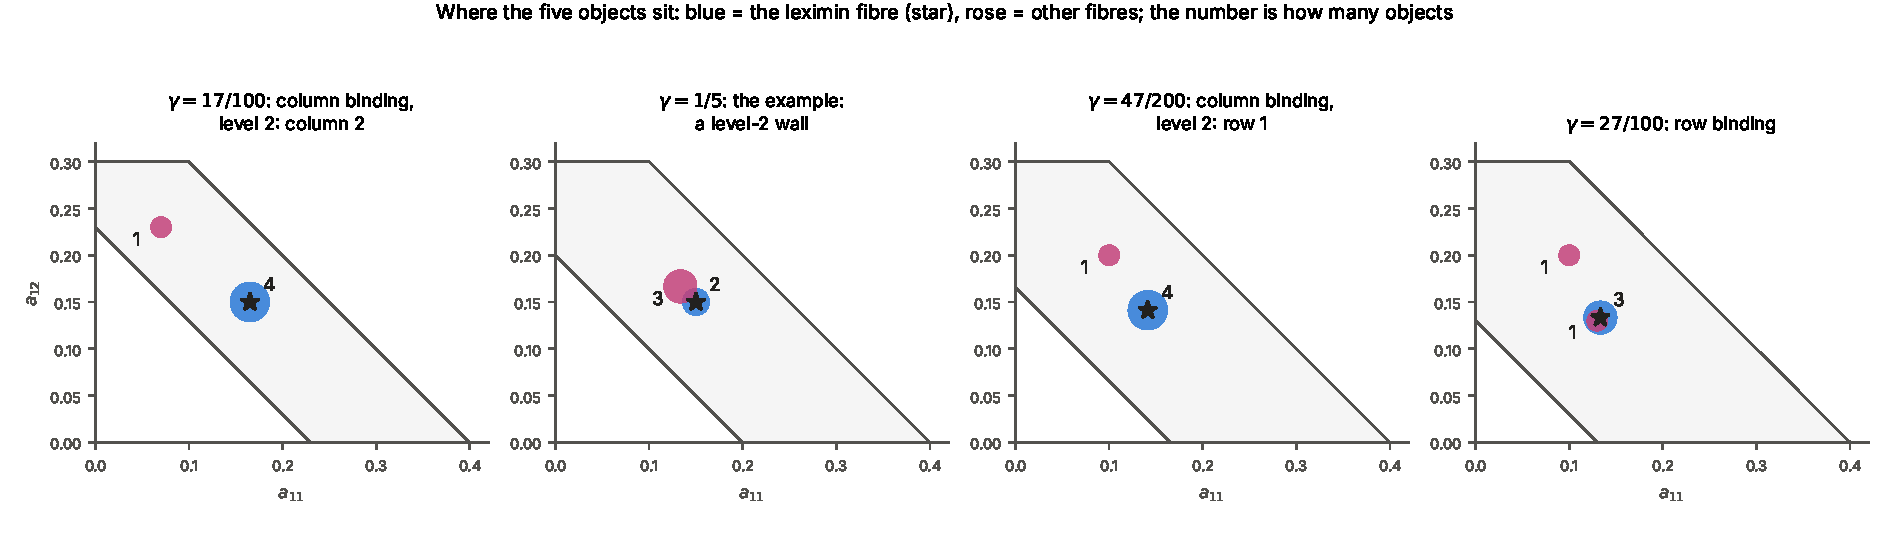
\includegraphics[width=\linewidth]{fig_s4_objects.pdf}
\caption{The five objects over the pentagon at four points of the path; the marker size and the number give how many objects sit over each fibre. Away from the wall $\gamma=1/5$ the leximin fibre (blue,
star) carries four objects, then three after the level-one wall.}\label{fig:s4objects}
\end{figure}

\begin{proposition}[what crosses each wall]\label{prop:crossing}
Along the path, at fixed small $T$:
\begin{enumerate}
\item[(1)] \emph{The level-two wall forces a collision.} At $\gamma=0.15$ and $0.18$ all five critical points are real; at $\gamma\ge0.22$, three are. The coefficients of \eqref{eq:pathquintic} are real and its leading coefficient $C$
never vanishes, so the number of real roots can change only through a double root. Numerically the discriminant has exactly one zero on the path, at $\gamma_c(T)$, for $T=e^{-50},e^{-100},e^{-200},e^{-400}$,
with $\gamma_c=0.19235$, $0.19918$, $0.199985$, $0.19999999$: it approaches the wall from below, faster than $1/\log(1/T)$. There the two objects of signs $(+,-)$ meet and leave as the complex pair
$I_\pm$. At that one parameter a critical point is degenerate.
\item[(2)] \emph{The level-one wall does not.} The discriminant has no zero on $(0.21,\,0.275]$. The pair $I_\pm$ continues into $C_\omega,C_{\bar\omega}$, and $N$ leaves the leximin fibre along the diagonal.
\item[(3)] \emph{Critical values} never coincide on the path away from the collision, and the order of the real values is constant on each side (PP7). So outside $\gamma_c(T)$ the hypotheses of
\cref{prop:morph} hold at every point: every off-diagonal Hom vanishes, and each endomorphism algebra is $\mathrm{Cl}(Q_c)\cong M_2(\Lambda)$.
\item[(4)] \emph{The Clifford shadow sees both walls} (\cref{fig:s4track}(b)). The positive object's scale is $h_2-h_1=3/20-\gamma/2$ below $1/5$ and $1/5-3\gamma/4$ above it, so the scale has a kink at the
level-two wall and closes at the level-one wall, where the reduced rank jumps from $1$ to $2$ (\cref{thm:shadow}). The four objects over the leximin fibre share this scale; $R$ has rank $2$
throughout.
\end{enumerate}
\end{proposition}

\begin{proof}
(1) Real-root counting, together with PP5 for the counts and PP6 for the zero. (2) PP6. (3) PP7, and \cref{prop:morph}(2)--(3). (4) PP8 compares the slopes at $L=400\to800$ with $h_2-h_1$ from
\cref{prop:path}(1).
\end{proof}

What (3) does and does not give needs saying plainly. At every parameter away from $\gamma_c(T)$ the five objects generate $\bigoplus_{c=1}^5\mathrm{Cl}(Q_c)$ over $\Lambda$, on both sides of the level-one wall. All
such categories are equivalent over $\Lambda$, so this pointwise statement says little. It is not an $A_\infty$ functor along the path, and non-collision alone would not give one. Over $\Lambda_0$ the
positive object changes across the level-one wall: its reduced Clifford form goes from rank $1$ to rank $2$. Across the level-two wall the path meets a degenerate critical point at $\gamma_c(T)$,
where the cited theorems do not apply.

\begin{figure}[!htbp]\centering
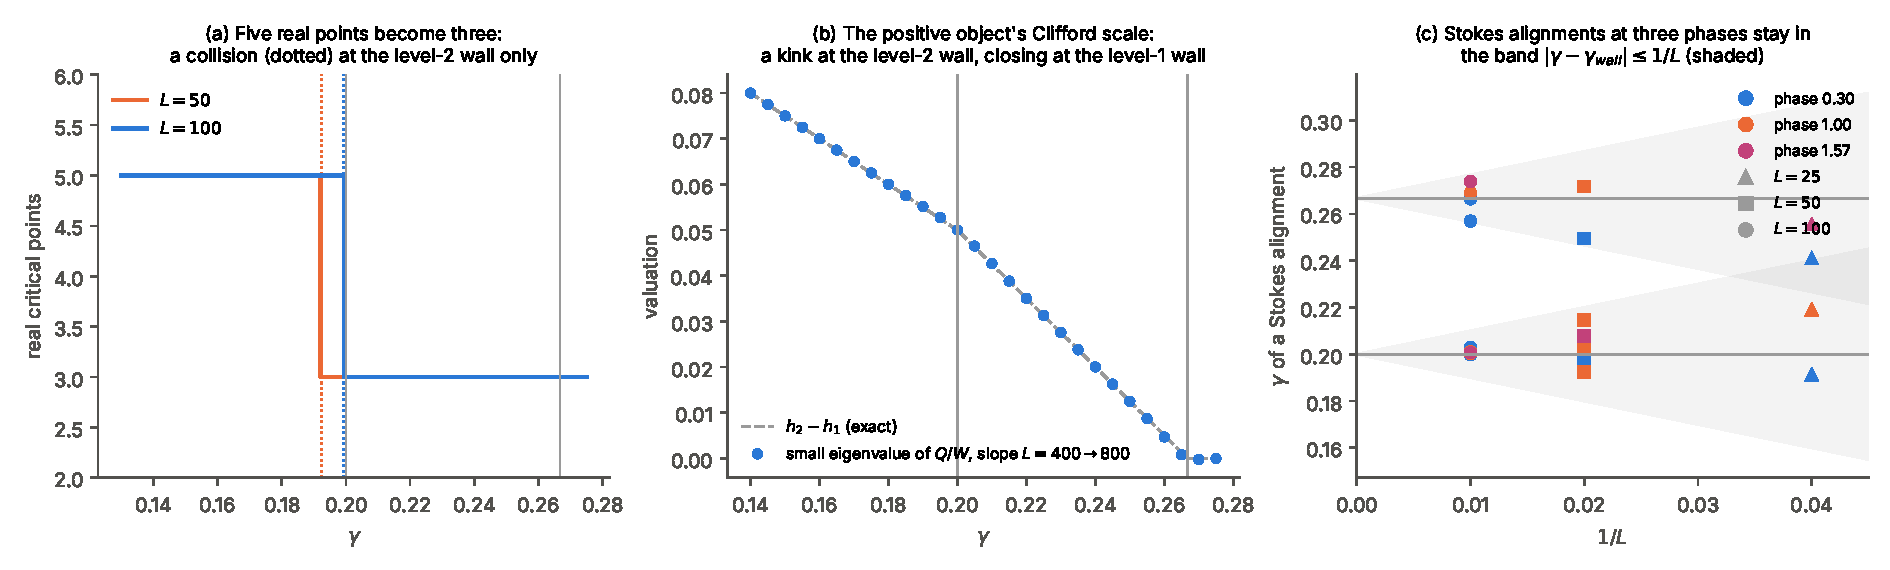
\includegraphics[width=\linewidth]{fig_s4_track.pdf}
\caption{Along the path. (a) The number of real critical points at $L=50$ and $100$; the dotted lines are the zeros of the discriminant, one per $L$, at the level-two wall. (b) The small eigenvalue of
$Q/W$ at the positive object, against $h_2-h_1$. (c) The positions of Stokes alignments at three phases and three values of $L$; the shaded bands are $|\gamma-\text{wall}|\le1/L$.}\label{fig:s4track}
\end{figure}

\paragraph{Stokes alignments, separately.} For the phases $\theta=0.3$, $1.0$ and $\pi/2$, and $L=25,50,100$, every parameter where two critical values align, $\operatorname{Im}e^{-i\theta}(W_j-W_i)=0$, lies
within $1.5/L$ of one of the two leximin walls, and at $L=100$ within $1/L$; alignments occur near both walls (PP9; \cref{fig:s4track}(c)). This is the behaviour of \cref{prop:stokes} on $F_1$, now
near two walls at once. We do not claim it for every phase, nor that every leximin wall has such alignments nearby; near the level-two wall some alignments involve the pair born at the collision.

\subsection{Composing couplings: Markov gluing and selection}\label{sec:selcomp}
The objects and morphisms of \cref{sec:morph} are cited from Floer theory. This subsection asks what composition the probabilistic side has of its own, and whether it has higher structure. It does not
produce an $A_\infty$ category. It separates a strict composition (the control) from one that is genuinely non-associative, and computes, exactly, the configuration that the associahedron $K_4$ then
carries.

\begin{definition}[couplings and two compositions]\label{def:selcomp}
An object is a finite set $X$ with a full-support law $p$; a morphism $(X,p)\to(Y,q)$ is a coupling $\gamma\in\Pi(p,q)$. For a chain $\gamma_1,\dots,\gamma_k$ of consecutive couplings, its \emph{fibre} is the
polytope of multi-couplings on $X_0\times\dots\times X_k$ with the consecutive pair marginals $\gamma_1,\dots,\gamma_k$.
\begin{enumerate}
\item[(1)] \emph{Markov gluing} composes by conditional independence over the shared marginal: $\gamma_2\circ\gamma_1=\gamma_1D_q^{-1}\gamma_2$, with $D_q=\operatorname{diag}(q)$.
\item[(2)] \emph{Selection} composes a block at once: $\sigma(\gamma_1,\dots,\gamma_k)$ is the marginal on $X_0\times X_k$ of the facet-leximin point of the fibre. By \cref{thm:selection}, applied to the fibre's
potential, this is the $T\to0$ limit of the positive critical point.
\end{enumerate}
\end{definition}

\begin{proposition}[the control: Markov gluing]\label{prop:markovglue}
\begin{enumerate}
\item[(1)] Markov gluing is associative and unital, with the diagonal coupling $D_p$ as identity.
\item[(2)] The Markov multi-coupling of a chain is the unique point of largest entropy in its fibre, and its $(X_0,X_k)$ marginal is the iterated composite.
\item[(3)] Every fibre is a nonempty convex polytope. So any assignment of points of $\Pi(p_0,p_n)$ to the faces of $K_n$ extends to a continuous map $K_n\to\Pi(p_0,p_n)$ (piecewise linear on the barycentric
subdivision) whose restriction to each face is determined by the points of that face. For Markov gluing every face receives the same point, so such fillers force no operation beyond the strict
composition.
\end{enumerate}
\end{proposition}

\begin{proof}
(1) Matrix multiplication, $(\gamma_1D^{-1}\gamma_2)D^{-1}\gamma_3=\gamma_1D^{-1}(\gamma_2D^{-1}\gamma_3)$, and $D_p\,D_p^{-1}\gamma=\gamma$. (2) By the chain rule, $H(X_0,\dots,X_k)\le H(X_0)+\sum_iH(X_i\mid X_{i-1})$, and the
right side is fixed by the pair marginals; equality holds exactly when the chain is Markov, and entropy is strictly concave. (3) The Markov point lies in the fibre, and the target is convex. AS1 checks
(1) and (2) in exact rationals, and that Markov gluing gives one composite on every face of $K_4$.
\end{proof}

This is the categorical-probability picture of Markov kernels \cite{Fritz2020}, restricted to couplings. Part (2) places it in this note: the Markov composite is the Birch point of the chain model's
fibre. Selection picks a different point of the same fibre, and that changes the composition law.

\paragraph{Faces as dissections.} A face of $K_n$ is a partial bracketing of $n$ morphisms, equivalently a dissection of the $(n+1)$-gon with vertices $0,\dots,n$, whose sides $(i,i+1)$ are the
$\gamma_{i+1}$ and whose root side $(0,n)$ is the output \cite{Stasheff1963}; combinatorially $K_n$ is the secondary polytope of the $(n+1)$-gon \cite{GKZ1994}. The composite along a dissection is
computed cell by cell: a cell with vertices $i_0<\dots<i_k$ is one selection in its own $(k+1)$-way table, whose consecutive margins are its sides, each an input or the composite of a smaller cell.
Vertices are full bracketings (binary selections), and the top cell is one selection in the $(n+1)$-way table. This is what makes face compatibility meaningful: the composite of a face is computed
from the composites of the blocks it contains, with their own margins. AS2 checks the face counts $3,11,45$ for $n=3,4,5$.

\begin{proposition}[selection: what holds and what fails]\label{prop:selprops}
Selection is unital (the diagonal coupling on either side returns the other) and commutes with transposition, $\sigma(\gamma_2^{\!\top},\gamma_1^{\!\top})=\sigma(\gamma_1,\gamma_2)^{\!\top}$. It is not associative:
on $30$ random rational chains of three couplings the two bracketings differ in $26$.
\end{proposition}

\begin{proof}
With a diagonal coupling the fibre is a single point. Transposition reverses the chain and preserves the fibre and its facets. The rest is AS5--AS6, in exact rationals.
\end{proof}

\begin{theorem}[the $K_4$ configuration, exactly]\label{thm:k4}
Take binary laws $p_0,\dots,p_4$ with first entries $2/5,1/3,3/7,1/4,5/11$, and the couplings $\gamma_1,\dots,\gamma_4$ with $a_{00}=13/60,7/30,1/80,3/80$. The eleven faces of $K_4$ receive the endpoint
couplings with these entries $a_{00}$:
\begin{center}\footnotesize
\begin{tabular}{lrlr}\toprule
vertex (bracketing) & $a_{00}$ & edge to the next vertex (block) & $a_{00}$\\\midrule
$((12)3)4$ & $173/960$ & $[0..3]$ & $997/5760$\\
$(1(23))4$ & $61/384$ & $[1..3]$ & $197/1152$\\
$1((23)4)$ & $61/320$ & $[1..4]$ & $14941/73920$\\
$1(2(34))$ & $38/165$ & $[2..4]$ & $1249/5280$\\
$(12)(34)$ & $93/385$ & $[0..2]$ & $15403/73920$\\\midrule
top: one selection in the $5$-way table & $28573/147840$ & Markov, every face & $2371469/12672000$\\\bottomrule
\end{tabular}
\end{center}
A block $[i..j]$ is one selection in the table over $X_i,\dots,X_j$.
The edge in each row joins that row's vertex to the next one, cyclically. All eleven are distinct, each edge composite lies strictly between its two vertices, and the top lies strictly inside
their range. Markov gluing gives the one value in the last cell on every face.
\end{theorem}

\begin{proof}
Each composite is computed level by level by linear programming and the leximin point is solved exactly from the fixed cells and the margins (AS3). Every selection used here then carries an exact
certificate (SX2): feasibility; the forced zeros and the dimension of the fibre; a witness face of dimension one less for each facet cell, and for every other cell an exact lower bound or a certified
extra zero; for each level a balanced law $q>0$ on the level set with $\sum_cq_ce_c$ in the row space of the margins and the earlier fixed cells, which bounds the level and forces the whole level set;
and strictly increasing levels. So the composites are certified, not only computed.
\end{proof}

The same holds with more states, and then the configuration can be seen in the plane. For $p_0=(2/5,3/5)$ and $p_4=(1/4,1/3,5/12)$, with ternary $p_1,p_3$ (\cref{fig:asconfig}(b)), the eleven
composites are distinct points of the two-dimensional polytope $\Pi(p_0,p_4)$, the top lies strictly inside the convex hull of the five bracketings, and the Markov composite lies outside it (AS4; exact
orientation tests and certified selections, SX2--SX3). The image of the pentagon crosses itself: the edge through block $[0..3]$ meets the one through $[2..4]$, and so does the edge through $[1..3]$. So the map $K_4\to\Pi(p_0,p_4)$ of \cref{prop:markovglue}(3), built from these composites, is a configuration and not an embedding, and since the target is
convex it carries no homotopy type of its own. Its content is where the eleven points sit.

\begin{figure}[!htbp]\centering
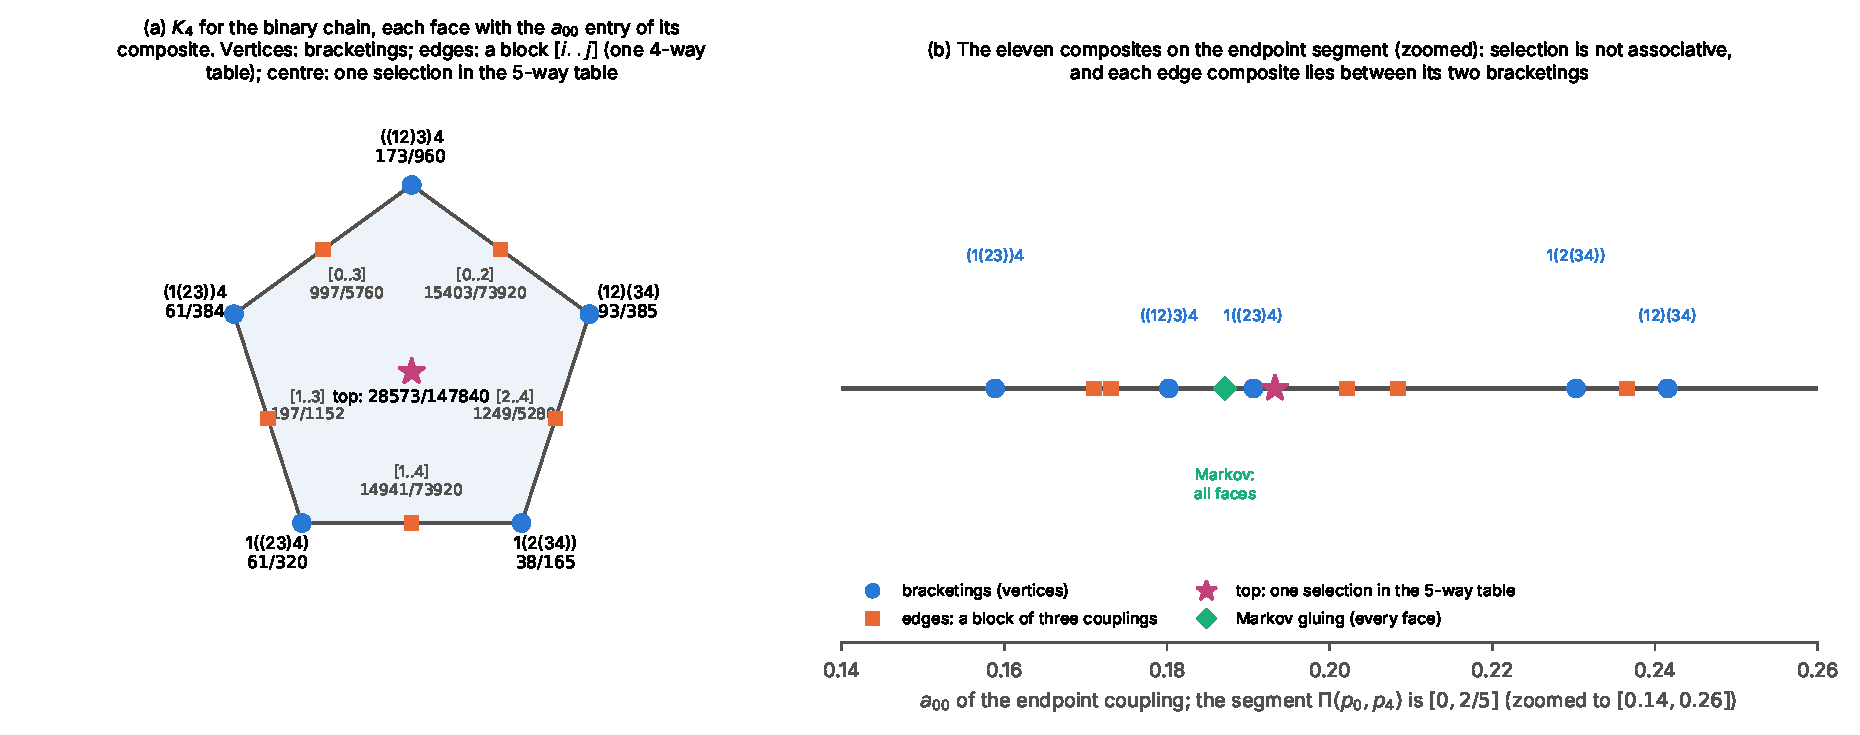
\includegraphics[width=\linewidth]{fig_as_pentagon.pdf}\\[4pt]
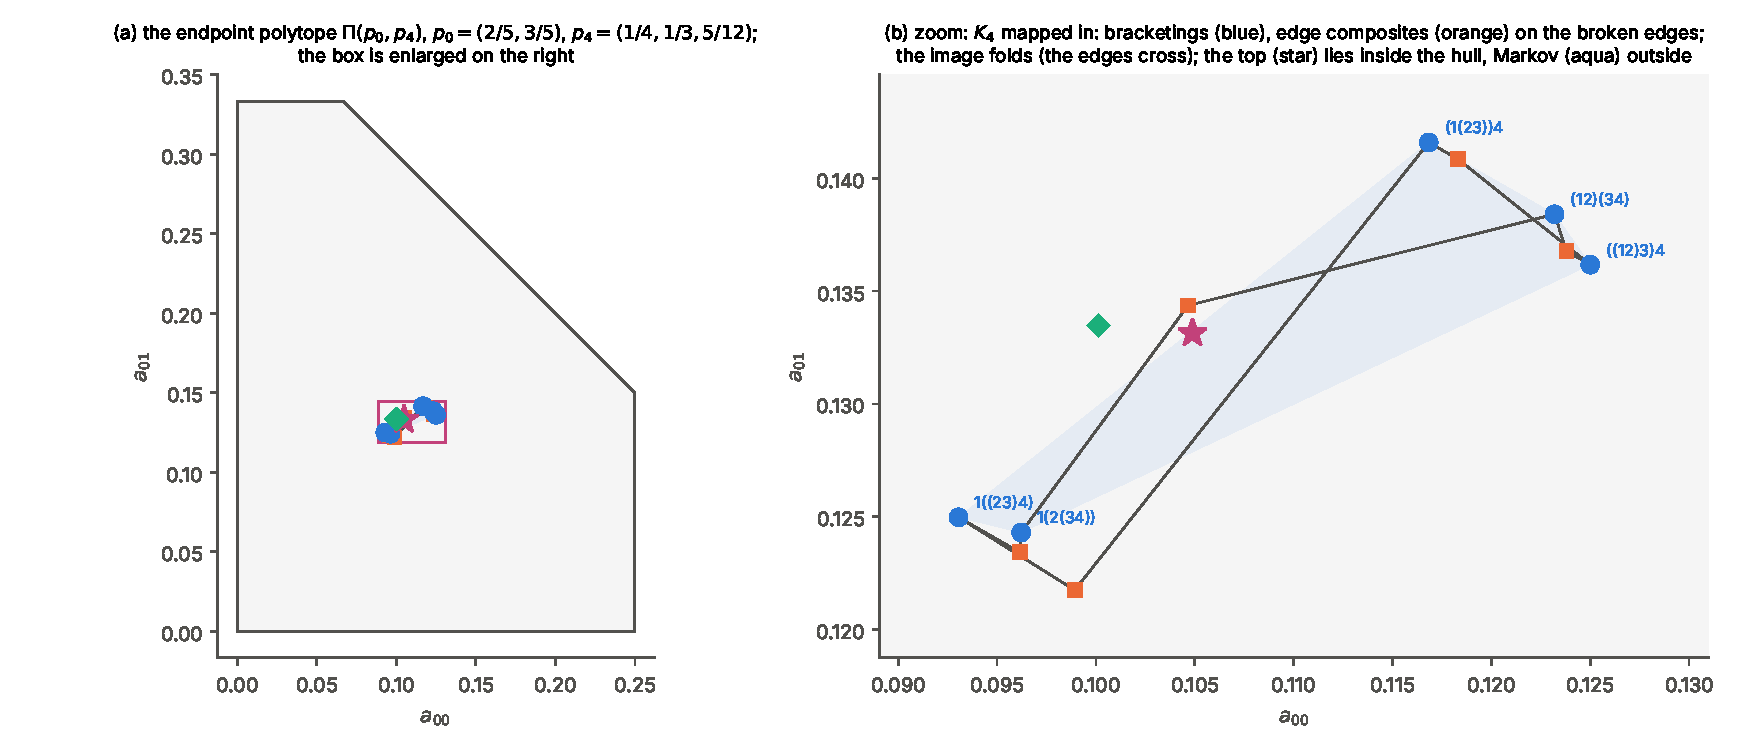
\includegraphics[width=\linewidth]{fig_as_polytope.pdf}
\caption{Composition by selection. Top: (a) $K_4$ for the binary chain of \cref{thm:k4}, each face labelled with its composite; (b) the eleven composites on the endpoint segment, with the single Markov
composite. Bottom: the chain with ternary intermediates; (a) the endpoint polytope; (b) $K_4$ mapped into it. The five bracketings (blue) and the five edge composites (orange) trace a folded pentagon;
the top (star) is inside the hull, the Markov composite (aqua) outside.}\label{fig:asconfig}
\end{figure}

\paragraph{Finite $T$.} Replace the facet-leximin point by the positive critical point at $T=e^{-L}$ on each fibre. On the first three couplings of \cref{thm:k4}, the two bracketings differ by $-41/960$ at
$L=25,50,100,200$, to $10^{-9}$: the binary composites already sit at their limits, and the top approaches its limit faster than $1/L$ (AS7). So the bracketings have no common leading term. The failure
of associativity is visible at the tropical level, not only at higher order in $T$.

\begin{remark}[what this does and does not give]\label{rem:selcomp}
An earlier draft conjectured that the associator might have a positive valuation, equal to a gap $h_j-h_1$ between selection levels, which would make it a candidate for a filtered $m_3$ that cannot be removed.
That form is refuted here: the associator is of order one. Two questions remain open. On the locus where the tropical bracketings agree, does the finite-$T$ associator have a $T$-adic valuation tied
to the level gaps? And, before any of this can be called an $A_\infty$ operation, one needs chain-level morphism complexes and a differential, with $m_3$ a specified homotopy between the two composites
that satisfies the next coherence relation. Nothing here constructs those. What is established is the vertex and face data that any such structure on selection would have to interpolate.
\end{remark}

\subsection{Selection: a no-go result, continuity, and binary chains}\label{sec:selbin}
Can the associator of \cref{sec:selcomp} be the $m_3$ of an $A_\infty$ category whose morphism complexes are chains on the coupling polytopes? It can be, formally, and the first result says why that
would carry no invariant. The rest of the subsection studies selection itself, where the information is.

\begin{proposition}[no-go for contractible morphism spaces]\label{prop:nogo}
Let $\mathcal C$ be an uncurved $A_\infty$ category over $\mathbb Q$, $\mathbb Z$- or $\mathbb Z/2$-graded, whose objects are finite probability spaces and whose morphism complexes have
$H^*(\hom(P,Q))\cong H_*(\Pi(p,q);\mathbb Q)$, for instance singular chains. Suppose $m_2$ induces on $H^0$ the composition of point classes, $[x]\cdot[y]=[\text{any composite}]$, with the class of the
diagonal coupling as unit. Then:
\begin{enumerate}
\item[(1)] the homology category has $\hom=\mathbb Q$ in degree $0$ for every pair of objects, composition $1\cdot1=1$, and every two objects are isomorphic;
\item[(2)] $\mathcal C$ is quasi-equivalent to the full subcategory on one object, and that is quasi-isomorphic to $\mathbb Q$ with $m_n=0$ for $n\ge3$.
\end{enumerate}
So no choice of $m_3,m_4,\dots$ on such complexes is an invariant up to quasi-equivalence. In particular the associator of selection is always a boundary there: the two bracketed composites are
points of one convex polytope, and the segment between them is a $1$-chain whose boundary is their difference. The proposition says nothing about categories built from coupling data in other ways.
\end{proposition}

\begin{proof}
(1) $\Pi(p,q)$ is nonempty and convex, so $H_*=\mathbb Q$ in degree $0$, spanned by the class of any point, and any composite of points is a point. Every class $1\in\hom(P,Q)$ has the inverse $1\in\hom(Q,P)$.
(2) A full subcategory meeting every isomorphism class of the homology category is quasi-equivalent to the whole. Its one object has cohomological endomorphisms $\mathbb Q\cdot1$; a cohomologically
unital $A_\infty$ algebra is quasi-isomorphic to a strictly unital minimal one \cite{Seidel2008}, whose underlying space is $\mathbb Q\cdot e$, and strict unitality gives $m_n(e,\dots,e)=0$ for $n\ge3$. This
holds for either grading.
\end{proof}

The exact data of \cref{thm:k4} are therefore data of the selection operation, not invariants of such a category. That redirects the work: to understand selection, and to look for higher structure
where the morphism spaces are not contractible (\cref{sec:outlook}).

\begin{theorem}[binary selection is Fr\'echet-midpoint gluing]\label{thm:frechet}
Let $X_0$ and $X_2$ be binary and $X_1$ any finite set, with couplings $\gamma_1\in\Pi(p_0,p_1)$ and $\gamma_2\in\Pi(p_1,p_2)$. For each $b\in X_1$ put $r_b=\gamma_1(0,b)$, $s_b=\gamma_2(b,0)$ and $q_b=p_1(b)$. Then
\[
\sigma(\gamma_1,\gamma_2)_{00}=\sum_b\frac{L_b+U_b}2,\qquad L_b=\max(0,\,r_b+s_b-q_b),\quad U_b=\min(r_b,s_b),
\]
the sum over $b$ of the midpoints of the Fr\'echet--Hoeffding intervals of the slices. Markov gluing gives $\sum_br_bs_b/q_b$ instead.
\end{theorem}

\begin{proof}
The pair-margin constraints involve one value of the middle variable at a time, so the fibre is the product over $b$ of the transportation polytopes of the slices $X_0\times\{b\}\times X_2$, with
margins $(r_b,q_b-r_b)$ and $(s_b,q_b-s_b)$. With $X_0,X_2$ binary each slice is the segment $x_{0b0}\in[L_b,U_b]$: the other three cells are $r_b-x_{0b0}$, $s_b-x_{0b0}$ and $q_b-r_b-s_b+x_{0b0}$, and the
Fr\'echet--Hoeffding bounds are where one of the four vanishes. A face of a product is a product of faces, so the facets of the fibre are the facets of single slices, and the facet functions of slice $b$
are $x_{0b0}-L_b$ and $U_b-x_{0b0}$, the cells that vanish at its ends (several cells when the slice is tied, all with the same function). A degenerate slice, $L_b=U_b$, is a point and contributes nothing.

Now run the recursion of \cref{def:lex}. Each facet function depends on one slice only, and the feasible set is a product. So at level $j$ the maximum of the least free function is the least, over the
slices with free functions left, of each slice's own next level; the slices attaining it fix their functions, and the others are untouched. By induction the recursion fixes, in each slice, exactly the
levels of that slice's own recursion, and the selected point is the product of the slices' selected points. On a segment with facet functions $x-L$ and $U-x$ that point is the midpoint, at level
$(U-L)/2$. SB1 checks the formula against the leximin computation on $60$ chains, including ternary middles and tied slices.
\end{proof}

So selection glues each slice at the midpoint between its comonotone and countermonotone couplings, where Markov gluing takes the product $r_bs_b/q_b$, which also lies in $[L_b,U_b]$. The two agree exactly
when the product sits at the midpoint of every slice. Two consequences follow at once. Since $L_b$ and $U_b$ are a maximum and a minimum of affine functions of the inputs, binary selection is continuous and
piecewise linear on the whole product of the coupling polytopes, with no exceptional walls. And on uniform margins it has a closed form.

\begin{corollary}[uniform margins: correlations compose by a signed minimum]\label{cor:tropcorr}
If $p_0=p_1=p_2=(1/2,1/2)$, write a coupling by its correlation $\rho=4\gamma_{00}-1$. Then
\[
\rho_{\mathrm{Markov}}=\rho_1\rho_2,\qquad \rho_{\mathrm{sel}}=\operatorname{sign}(\rho_1\rho_2)\,\min(|\rho_1|,|\rho_2|).
\]
In $v=-\log|\rho|$, Markov gluing adds and selection takes the maximum. On uniform binary chains selection is therefore associative, with unit $\rho=1$.
\end{corollary}

\begin{proof}
With $q=1/2$, \cref{thm:frechet} gives $\gamma_{00}-\tfrac14=\tfrac12\bigl(|t_1+t_2-\tfrac12|-|t_1-t_2|\bigr)$ for $t_i=\gamma_{i,00}$, which is $\operatorname{sign}(d_1d_2)\min(|d_1|,|d_2|)$ with $d_i=t_i-\tfrac14$. The signed minimum is
associative. SB2 checks both laws and associativity on a $21^3$ grid, exactly.
\end{proof}

\begin{proposition}[where selection is associative]\label{prop:assoclocus}
For binary chains $\gamma_1,\gamma_2,\gamma_3$ with margins $p_0,\dots,p_3$, the associator $A=\sigma(\sigma(\gamma_1,\gamma_2),\gamma_3)-\sigma(\gamma_1,\sigma(\gamma_2,\gamma_3))$ is the explicit piecewise-linear function obtained by composing
\cref{thm:frechet} with itself. Moreover:
\begin{enumerate}
\item[(1)] among the $9^4$ margin tuples with entries in $\{1/10,\dots,9/10\}$, only the uniform one makes $A$ vanish on the whole test grid (a $5^3$ screen leaves $17$; a $13^3$ grid leaves one);
\item[(2)] for non-uniform margins $A$ can vanish on a set of positive volume: for the margins $2/5,1/3,3/7,1/4$ of \cref{thm:k4}, $A=0$ on the open polyhedron of all $(t_1,t_2,t_3)$ for which the $22$
  branch and feasibility inequalities of the formula keep the signs they have at $(13/60,\,7/30,\,29/240)$; likewise for the margins $3/20,1/4,3/4,17/20$ around $(1/40,\,1/48,\,51/80)$;
\item[(3)] on exact $13^3$ grids, $A=0$ at between $15\%$ and $55\%$ of the points for six non-uniform tuples, and this set is not a union of classes of the dependence signs $\operatorname{sign}(t_i-p_ip_{i+1})$.
\end{enumerate}
\end{proposition}

\begin{proof}
The formula is \cref{thm:frechet}. (2) At the given point every maximum and minimum in the formula is strict, so the same branches hold on the open polyhedron, where $A$ is affine; its four coefficients
are all zero, and the point lies inside, so the polyhedron has nonempty interior (SX1, exact). (1) and (3) are exact evaluations on rational grids, SB5--SB6; they are a census, not a classification of the
locus.
\end{proof}

\begin{example}[one parameter, exactly]\label{ex:assoc1}
Take the margins $2/5,1/3,3/7,1/4$ of \cref{thm:k4} with $t_1=13/60$, $t_2=7/30$, and let $t_3$ run over $[0,1/4]$. Then $A(t_3)$ is piecewise linear with kinks at $1/30$, $13/120$, $2/15$, $3/20$, $143/840$, $41/210$, $7/30$
and slopes in $\{0,\pm\tfrac14,\tfrac12\}$. It vanishes exactly on the interval $[13/120,2/15]$ and at the point $5/28$, changes sign there, and equals $-41/960$ at $t_3=1/80$, the example of
\cref{sec:selcomp} (\cref{fig:sb}(b); SB7). The interval is a slice of the full-dimensional cell of \cref{prop:assoclocus}(2). Independence, $t_3=3/28$, lies just outside it; we know no reason for
this and record it only as an observation.
\end{example}

\paragraph{Continuity in general.} On a region of inputs where the facet set and the level sets $S_1,\dots,S_J$ of the recursion are fixed, the selected point is the unique solution of a linear system
whose matrix is fixed and whose right side is linear in the inputs, so selection is affine there (SB3 checks this exactly at $339$ midpoints). Across changes of the facet set we have only evidence:
along four paths of a $3\times2\times3$ chain the facet set changes at least ten times, and the composite never jumps (SB4; \cref{fig:sb}(c)). A proof of continuity across these walls is open.

\begin{figure}[!htbp]\centering
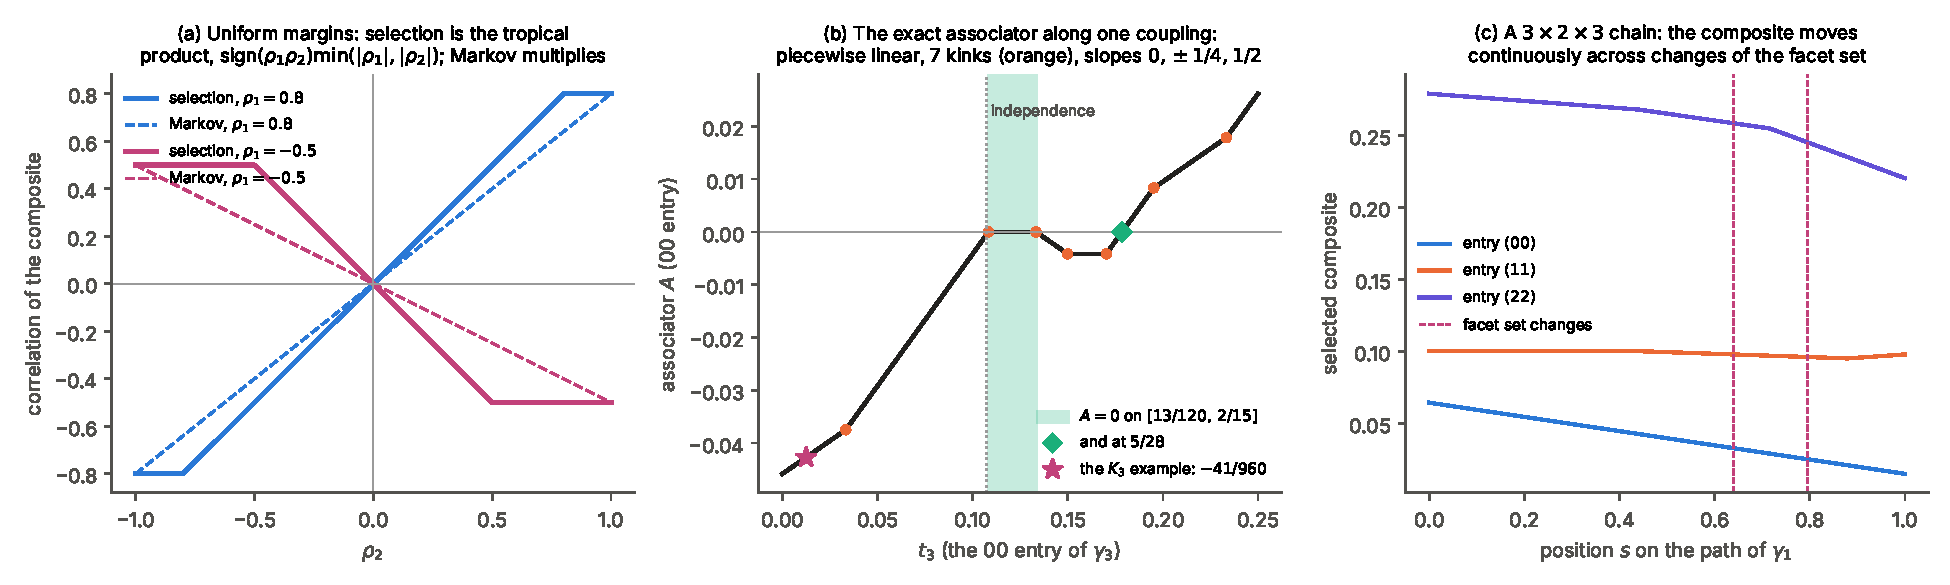
\includegraphics[width=\linewidth]{fig_sb.pdf}
\caption{Selection on small chains. (a) Uniform binary margins: correlations compose by a signed minimum under selection and by a product under Markov gluing. (b) The exact associator of
\cref{ex:assoc1}, with its kinks, its interval and point of associativity, and the value $-41/960$ of \cref{sec:selcomp}. (c) The selected composite along a path of a $3\times2\times3$ chain; the dashed lines are
changes of the facet set, where nothing jumps.}\label{fig:sb}
\end{figure}

\subsection{A Floer reading of selection, at the level of objects}\label{sec:selfloer}
Composition of couplings is reduction in stages. The tables over $X_0\times X_1\times X_2$ with pair marginals $\gamma_1,\gamma_2$ form the fibre polytope $F(\gamma_1,\gamma_2)$; when it is Delzant it is the moment
polytope of a toric manifold $X_F$, a symplectic reduction of the manifold of all tables. Both compositions pick a point of $F$ and then take its $(X_0,X_2)$ marginal. Markov gluing picks the point of
largest entropy, the Birch point (\cref{prop:markovglue}(2)). Selection picks the facet-leximin point, which by \cref{thm:selection} is the valuation of the positive critical point of the potential of $X_F$. The
fibre over that point is the non-displaceable torus fibre that Fukaya, Oh, Ohta and Ono locate in any compact toric manifold \cite[Theorem~1.5 and \S9]{FOOO2010}, by the recursion of \cref{def:lex}
(\cref{sec:selection}, the remark on provenance). For binary chains this can be said exactly, and on both sides of Floer theory.

\begin{proposition}[binary selection picks the Floer-nontrivial fibre]\label{prop:selfloer}
Let $X_0$ and $X_2$ be binary, and let $k$ be the number of slices $b$ with $L_b<U_b$ (\cref{thm:frechet}). Then $X_F\cong\prod_b\mathbb{CP}^1$, with areas $U_b-L_b$, which is Fano, and for a torus fibre $L_c$:
\begin{enumerate}
\item[(1)] $L_c$ carries a unitary local system with $HF\ne0$ if and only if $c$ is the product of the slice midpoints; there are $2^k$ such objects, $y_b=\pm T^{(U_b-L_b)/2}$ in slice coordinates \cite{ChoOh2006};
\item[(2)] with local systems $\rho$ valued in $\overline{\mathbb F}_2^{\,*}$, $HF(R,(L_c,\rho))\ne0$ for the real Lagrangian $R$ if and only if $c$ is the product of the midpoints; then $\rho=1$ and $HF(R,L_c)$ is free of
rank $2^k$ \cite[Theorems~1.2 and 4.3]{AlstonAmorim2010}.
\end{enumerate}
So $\sigma(\gamma_1,\gamma_2)$ is the $(X_0,X_2)$ marginal of the unique torus fibre of $X_F$ that is Floer-nontrivial, on its own or against $R$. The Markov composite is the marginal of the Birch point of the
same polytope, $c_b=r_bs_b/q_b$, which is a different point in $37$ of $40$ chains tested.
\end{proposition}

\begin{proof}
By the proof of \cref{thm:frechet}, $F=\prod_b[L_b,U_b]$ over the nondegenerate slices, with facet functions $x_b-L_b$ and $U_b-x_b$ of primitive normals $\pm1$; so $X_F=\prod_b\mathbb{CP}^1$, and SF1 confirms by
exact traversal that $F$ is Delzant with $2^k$ vertices and $-K\cdot C=2$ on every invariant curve. In slice coordinates the potential is $W=\sum_b(y_b+T^{w_b}/y_b)$ with $w_b=U_b-L_b$. (1) Its critical points are
$y_b=\pm T^{w_b/2}$, over the midpoints, and Cho--Oh identify the fibres with $HF\ne0$ with the valuations of critical points (SF2). (2) Alston--Amorim show $HF(R,(L_c,\rho))\ne0$ if and only if
$\nabla W_c(\rho)=0$. In characteristic $2$ the $b$-th component is $\rho_bT^{c_b-L_b}+\rho_b^{-1}T^{U_b-c_b}$, which vanishes only if the exponents agree and $\rho_b^2=1$, that is $c_b$ is the midpoint and $\rho_b=1$.
There their differential $\sum_j\sqrt{\rho^{v_j}}\,T^{E_j/2}f_j$ is $\sum_b2T^{w_b/4}f_b=0$, so the complex, free of rank $2^k$, is its own cohomology (SF3). SF4 compares the Birch points.
\end{proof}

\begin{remark}[what this explains, and how far it goes]\label{rem:selfloer}
\emph{Non-associativity.} Reduction in stages is associative; choosing a point is not compatible with it in general. Birch points are, which is why Markov gluing is associative. Floer fibres are not:
$\sigma(\sigma(\gamma_1,\gamma_2),\gamma_3)$ takes the Floer fibre of one reduced space and reduces again, while the top cell takes the Floer fibre of the larger reduced space at once.

\emph{Beyond binary.} For the binary $K_4$ example the fibres behind the eleven composites are, by exact traversal (SF5): the $14$ distinct $3$-way fibres are each $\mathbb{CP}^1\times\mathbb{CP}^1$, so
\cref{prop:selfloer} applies; of the $5$ distinct $4$-way fibres, three are Delzant and two are simple but not unimodular, so the toric variety is an orbifold, and none is Fano (a curve with $-K\cdot C=-4$);
the $5$-way fibre of the top cell is not Fano either: a complete exact traversal ($34\,166$ vertices) finds it simple but not unimodular, so an orbifold, with a curve of $-K\cdot C=-32$. For the Delzant ones the selected point is the FOOO non-displaceable fibre. The
equivalences (1) and (2) need the Fano hypothesis and are not claimed there, and the orbifold fibres would need orbifold Floer theory.

\emph{What is not claimed.} This reads selection at the level of objects, one torus fibre per composite. It constructs no functor and says nothing about morphisms or products between these fibres; the
categorical comparison of \cref{sec:threecat} is untouched. The real Lagrangian enters only through \cite{AlstonAmorim2010}; that it corresponds to hard evidence is a hypothesis we do not test.
\end{remark}

\subsection{Three categorical directions, kept apart}\label{sec:threecat}
Part III has touched three different constructions. They should not be confused.
\begin{center}\small
\begin{tabular}{p{0.2\linewidth}p{0.36\linewidth}p{0.36\linewidth}}\toprule
construction & what is established here & what is missing\\\midrule
the toric-fibre category & objects are critical points of $W$ over torus fibres; binary selection is read as the Floer-nontrivial fibre of the reduced space (\cref{prop:selfloer}); Hom vanishes off the diagonal where the critical values differ; the endomorphisms are Clifford algebras; no higher
products (\cref{prop:morph,prop:formal}); all cited, in the convention of \cref{sec:cbclass} & generation in the non-monotone case \cite{Smith2018}; the category at a collision (\cref{prop:crossing}) \\
a coupling-polytope enhancement & Markov and selection compositions, the exact $K_4$ data (\cref{sec:selcomp}); with point-class composition and diagonal units it is trivial up to quasi-equivalence
(\cref{prop:nogo}) & nothing to add in that form; another enhancement would need morphism spaces that are not contractible \\
a Fukaya--Seidel category of $W$ & only its combinatorial shadow: the critical points, their values, and where Stokes alignments occur (\cref{prop:stokes}, \cref{sec:path}) & gradings; Floer complexes
between thimbles; the polygon counts that define $\mu^d$; the directed $A_\infty$ structure \cite{Seidel2008}; and a proof that the positive thimble is the probabilistic object in that category\\\bottomrule
\end{tabular}
\end{center}

\subsection{A small dagger category for finite probability}\label{sec:probcat}
The underlying category here is standard. What is new is a precise account of which of its symmetries selection keeps and which it breaks. Write
$\gamma\otimes\gamma'$ for the Kronecker product of couplings, and $D_p=\operatorname{diag}(p)$.

\begin{definition}[the category $\mathsf{Cpl}$]\label{def:cpl}
Objects are finite sets with full-support laws $(X,p)$ (a state of mass zero is deleted). A morphism $(X,p)\to(Y,q)$ is a coupling $\gamma\in\Pi(p,q)$; composition is Markov gluing
$\gamma_1D_q^{-1}\gamma_2$, with identity $D_p$ (\cref{def:selcomp}). The dagger is the transpose, $\gamma^\dagger=\gamma^{\!\top}\in\Pi(q,p)$. The tensor product is $(X,p)\otimes(Y,q)=(X\times Y,p\otimes q)$ on objects and
$\gamma\otimes\gamma'$ on morphisms, with the swap of factors as symmetry. A coarse-graining of $(Z,r)$ along a map $f:Z\to Z'$ sends $\delta$ to $\delta F$, where $F$ is the $0/1$ matrix of $f$.
\end{definition}

Writing $K=D_p^{-1}\gamma$ turns couplings into Markov kernels that carry $p$ to $q$, and the transpose becomes Bayesian inversion \cite{Fritz2020,ChoJacobs2019}.

\begin{proposition}[the structure Markov gluing carries]\label{prop:cplcat}
$\mathsf{Cpl}$ is a dagger symmetric monoidal category, and Markov gluing commutes with coarse-graining an end space: $(\gamma D^{-1}\delta)F=\gamma D^{-1}(\delta F)$.
\end{proposition}

\begin{proof}
Associativity and units are \cref{prop:markovglue}(1). $(\gamma_1D^{-1}\gamma_2)^{\!\top}=\gamma_2^{\!\top}D^{-1}\gamma_1^{\!\top}$ and $D_p^{\!\top}=D_p$, so the transpose is an identity-on-objects involution that reverses composition. The mixed-product rule gives
$(\gamma\otimes\gamma')(D\otimes D')^{-1}(\delta\otimes\delta')=(\gamma D^{-1}\delta)\otimes(\gamma'D'^{-1}\delta')$ and $(\gamma\otimes\gamma')^{\!\top}=\gamma^{\!\top}\otimes\gamma'^{\!\top}$. The last identity is associativity of matrix
multiplication. NC1 checks all of these in exact rationals on random chains.
\end{proof}

\begin{example}[forecast, umbrella, wet]\label{ex:umbrella}
Let $X$ say whether the forecast is rain, $Y$ whether an umbrella is carried, $Z$ whether one gets wet, with $P(\text{rain})=2/5$, $P(\text{carried})=1/3$, $P(\text{wet})=3/7$. Two separate data sets record
the pairs:
\[
\gamma_1=\begin{pmatrix}13/60&11/60\\7/60&29/60\end{pmatrix}\in\Pi(X,Y),\qquad \gamma_2=\begin{pmatrix}7/30&1/10\\41/210&33/70\end{pmatrix}\in\Pi(Y,Z),
\]
rows and columns in the order (yes, no). No record contains all three. The two compositions give different laws for (forecast, wet):
\[
\gamma_1D_q^{-1}\gamma_2=\begin{pmatrix}23/112&109/560\\25/112&211/560\end{pmatrix},\qquad \sigma(\gamma_1,\gamma_2)=\begin{pmatrix}31/120&17/120\\143/840&361/840\end{pmatrix}.
\]
These are the first two couplings of \cref{thm:k4}. \Cref{fig:selcat} draws them, together with the two squares of \cref{prop:selbreaks}.
\end{example}

\begin{proposition}[what selection keeps]\label{prop:selkeeps}
For $\gamma\in\Pi(p,q)$ and $\delta\in\Pi(q,r)$:
\begin{enumerate}
\item[(1)] \emph{closed:} $\sigma(\gamma,\delta)\in\Pi(p,r)$;
\item[(2)] \emph{unital:} $\sigma(\gamma,D_q)=\gamma$ and $\sigma(D_p,\gamma)=\gamma$;
\item[(3)] \emph{reversal:} $\sigma(\gamma,\delta)^{\!\top}=\sigma(\delta^{\!\top},\gamma^{\!\top})$;
\item[(4)] \emph{relabelling:} for bijections $\alpha,\beta,\kappa$ of $X,Y,Z$, selection of the relabelled couplings is the relabelled selection;
\item[(5)] \emph{a copied factor:} for every full-support law $w$, $\sigma(\gamma\otimes D_w,\ \delta\otimes D_w)=\sigma(\gamma,\delta)\otimes D_w$.
\end{enumerate}
\end{proposition}

\begin{proof}
(1) The end marginal of a table with pair marginals $\gamma,\delta$ has margins $p$ and $r$. (2) is \cref{prop:selprops}. (3) and (4): the maps $x_{ijk}\mapsto x_{kji}$ and
$x_{ijk}\mapsto x_{\alpha(i)\beta(j)\kappa(k)}$ carry the fibre bijectively onto the fibre of the transformed chain. They preserve every cell value, so they preserve the facets and each step of
\cref{def:lex}; the leximin point is unique, so it goes to the leximin point. (5) The pair marginal $\gamma\otimes D_w$ forces $x_{(i,a),(j,b),(k,c)}=0$ unless $a=b$, and $\delta\otimes D_w$ forces $b=c$. So the
fibre is the product over $a$ of the scaled copies $w_aF(\gamma,\delta)$, through $x_{(i,a),(j,a),(k,a)}=w_ay^{(a)}_{ijk}$. Its facets are facets of single copies, and the facet functions of copy $a$ are $w_a$
times those of $F(\gamma,\delta)$. As in the proof of \cref{thm:frechet}, the recursion on a product whose facet functions each depend on one factor selects the product of the factors' own selected points. Scaling all
of a factor's functions by $w_a>0$ does not change that factor's selected point. NC2 and NC3 check (1)--(5) exactly.
\end{proof}

\begin{proposition}[what selection breaks]\label{prop:selbreaks}
With $\gamma_1,\gamma_2$ of \cref{ex:umbrella}:
\begin{enumerate}
\item[(1)] \emph{An independent factor.} With $\gamma'=\left(\begin{smallmatrix}1/5&1/20\\3/10&9/20\end{smallmatrix}\right)$ and $\delta'=\left(\begin{smallmatrix}1/10&2/5\\1/2&0\end{smallmatrix}\right)$, the $00$ entry of
$\sigma(\gamma_1\otimes\gamma',\gamma_2\otimes\delta')$ is $29/1400$, while that of $\sigma(\gamma_1,\gamma_2)\otimes\sigma(\gamma',\delta')$ is $31/1200$. So selection is not monoidal.
\item[(2)] \emph{Coarse-graining an end.} With $\delta=\left(\begin{smallmatrix}1/10&1/10&2/15\\1/5&1/5&4/15\end{smallmatrix}\right)$, merging the last two states of $Z$ after selection gives $00$ entry $11/90$, and merging them
before gives $17/120$.
\item[(3)] \emph{Coarse-graining the middle} changes both compositions. Markov gluing: for $\gamma=\left(\begin{smallmatrix}1/10&1/10&1/5\\1/5&3/20&1/4\end{smallmatrix}\right)$, $\delta=\left(\begin{smallmatrix}1/5&1/10\\1/20&1/5\\1/5&1/4\end{smallmatrix}\right)$,
merging the last two middle states moves the $00$ entry from $79/450$ to $73/420$. Selection: for $\gamma=\left(\begin{smallmatrix}1/8&9/32&3/32\\3/16&1/4&1/16\end{smallmatrix}\right)$,
$\delta=\left(\begin{smallmatrix}5/144&5/18\\85/448&153/448\\5/64&5/64\end{smallmatrix}\right)$, it moves from $1283/8064$ to $305/2016$, and it moves on $10$ of $15$ random chains.
\end{enumerate}
In (1) and (2) Markov gluing passes both squares (\cref{prop:cplcat}).
\end{proposition}

\begin{proof}
Exact computation, with every input above (NC4--NC6).
\end{proof}

Why Markov passes the tensor square and selection does not: the product chain's fibre contains $F(\gamma,\delta)\times F(\gamma',\delta')$ and also tables that are not products. For any table $x$ in it, with marginals
$x_1,x_2$ on the two systems, $H(x)\le H(x_1)+H(x_2)\le H(m)+H(m')$, where $m,m'$ are the Markov points of the factors. Equality holds at $m\otimes m'$, so the maximum-entropy point of the product is the product
of the maximum-entropy points. A least cell has no such inequality, and in (1) the leximin point of the product fibre is not a product.

\begin{center}\small
\begin{tabular}{lcc}\toprule
property & Markov gluing & selection\\\midrule
associative & yes & no (\cref{prop:selprops,thm:k4})\\
unital; reversal (dagger); relabelling & yes & yes\\
tensoring by an identity $D_w$ (a copied factor) & yes & yes\\
tensoring by an independent factor & yes & no\\
coarse-graining an end space & yes & no\\
coarse-graining the middle space & no & no\\
the point of the fibre it picks & largest entropy & lexicographically largest least slack\\\bottomrule
\end{tabular}
\end{center}

\begin{remark}[status]\label{rem:selcat}
So selection is a geometric rule on fibres. It is unchanged by renaming states, by reversing direction and by copying information, but it changes when an independent system is added or an end is recorded
at another resolution. Markov gluing is unchanged by all of these, and both change with the resolution of the middle. Together with the associator and the $K_4$ configuration, this is further evidence that
selection does not give $\mathsf{Cpl}$ a second composition law; nothing here alters the three directions of \cref{sec:threecat}.
\end{remark}

\begin{figure}[!htbp]\centering
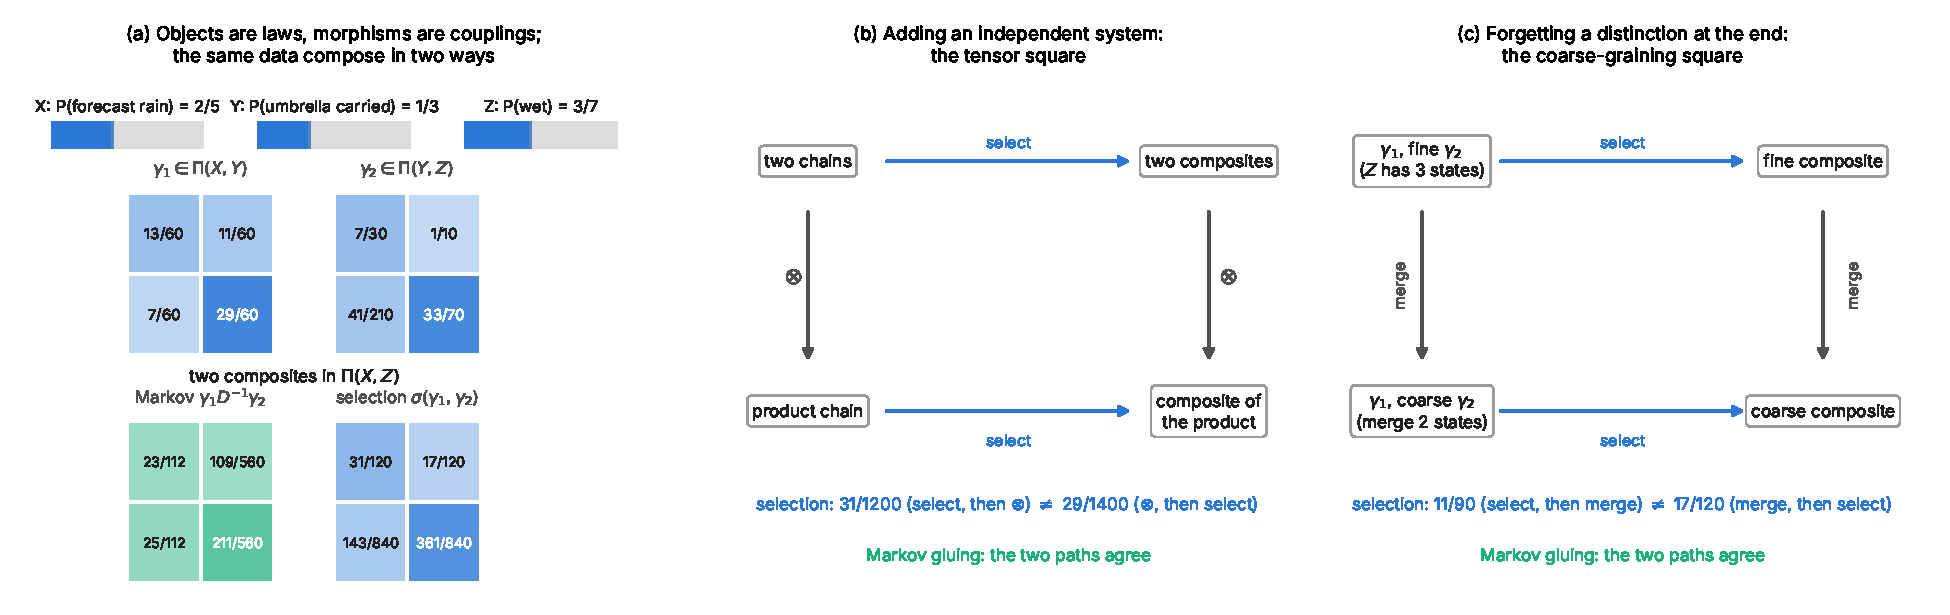
\includegraphics[width=\linewidth]{fig_selcat.pdf}
\caption{The small category on \cref{ex:umbrella}. (a) Three binary laws, the two data sets, and the two composites they give. (b) The tensor square: selecting and then taking the product differs from selecting on
the product chain. (c) The coarse-graining square: merging two end states before or after selection gives different answers. Markov gluing passes both squares.}\label{fig:selcat}
\end{figure}

\subsection{How little it takes: poisoning, representation, and what the data determine}\label{sec:howlittle}
In \cref{ex:umbrella} take the decision ``warn that rain is coming with you'' when $P(\text{wet}\mid\text{forecast rain})\ge\tau=1/2$, computed from a composite. This subsection asks how little has to change
for that decision to flip. Two kinds of change are compared: edits of the data themselves (poisoning), and changes in the representation underneath that leave the data as recorded untouched. For binary ends,
what the data alone determine has a closed form.

\begin{proposition}[what the data determine]\label{prop:identified}
Let $X_0$ and $X_2$ be binary, and use the notation of \cref{thm:frechet}.
\begin{enumerate}
\item[(1)] The $00$ entries of the $(X_0,X_2)$ marginals of all joint laws compatible with $\gamma_1$ and $\gamma_2$ fill the interval $[L,U]=[\sum_bL_b,\ \sum_bU_b]$.
\item[(2)] Selection is its midpoint. So among all rules it has the least worst-case error over compatible joint laws, namely $(U-L)/2$. Markov gluing has worst-case error $\max(u_M-L,\,U-u_M)$, which is
larger unless $u_M$ is the midpoint.
\item[(3)] Splitting a middle state into two, consistently with the recorded data, can only shrink $[L,U]$.
\item[(4)] The data alone decide the threshold question exactly when $\tau p_0\notin(L,U)$, with $p_0=P(X_0=0)$.
\end{enumerate}
\end{proposition}

\begin{proof}
(1) By the proof of \cref{thm:frechet} the fibre is $\prod_b[L_b,U_b]$, and the $00$ entry of the end marginal is $\sum_bx_{0b0}$. (2) The first claim is \cref{thm:frechet}, and the midpoint of an interval
minimises the largest distance to its points. (3) Merging the two halves of the split state sends a compatible table of the refined chain to a compatible table of the original one, with the same end marginal.
(4) follows from (1). NC7 checks (1) and (2) against linear programs over the fibre on $20$ chains, and NC9 checks (3) on $195$ refinements.
\end{proof}

In this language the interval is the \emph{identified set} of the composite \cite{Manski2003}. Neither composite is determined by the data: Markov gluing adds conditional independence given $Y$, and
selection takes the centre.

\begin{proposition}[edits inside the data]\label{prop:poison}
On binary chains, write $p_0,p_1,p_2$ for the first entries of the laws and $t_1,t_2$ for the $00$ entries of $\gamma_1,\gamma_2$. Change $\gamma_1$ by a margin-preserving swap of size $s$ (the $00$ and $11$ entries up by $s$, the others down). This moves $2|s|$ of the mass, so $2|s|$ is the fraction of records edited.
\begin{enumerate}
\item[(1)] The Markov composite is affine in $s$ with slope $(t_2-p_1p_2)/(p_1(1-p_1))$, which is proportional to the covariance in $\gamma_2$.
\item[(2)] The selected composite is piecewise linear in $s$, with slopes in $\{0,\pm\tfrac12,\pm1\}$. Its slope is $0$ on the open region where $t_1+t_2<p_1$, $t_2<t_1$, $(p_0-t_1)+(p_2-t_2)<1-p_1$ and $p_2-t_2<p_0-t_1$:
there, edits of $\gamma_1$ do not move it at all.
\end{enumerate}
\end{proposition}

\begin{proof}
(1) Differentiate $t_1t_2/p_1+(p_0-t_1)(p_2-t_2)/(1-p_1)$. (2) Each slice midpoint $(L_b+U_b)/2$ is a half-sum of a maximum and a minimum of affine functions with slope $0$ or $\pm1$ in $t_1$. Under the four
inequalities, $L_0=0$, $U_0=t_2$, $L_1=0$ and $U_1=p_2-t_2$, none of which depends on $t_1$.
\end{proof}

\begin{example}[how little, both ways]\label{ex:howlittle}
In \cref{ex:umbrella}, in units of $P(\text{wet}\mid\text{forecast rain})$:
\begin{enumerate}
\item[(1)] \emph{The data.} They determine only $[7/24,\,1]$, which contains $\tau$. Markov gluing gives $115/224\approx0.513$, worst-case error $109/224\approx0.487$. Selection gives $31/48\approx0.646$, worst-case error
$17/48\approx0.354$. Both warn.
\item[(2)] \emph{Poisoning.} The smallest margin-preserving edits that flip each decision are, as fractions of records edited:
\begin{center}\small
\begin{tabular}{lcc}\toprule
& edit $\gamma_1$ & edit $\gamma_2$\\\midrule
Markov stops warning & $1/38\approx2.6\%$ & $1/35\approx2.9\%$\\
selection stops warning & $9/70\approx12.9\%$ & $2/15\approx13.3\%$\\
the data force ``warn'' ($L\ge\tau p_0$) & $1/6\approx16.7\%$ & $1/6\approx16.7\%$\\
the data force ``no warning'' ($U\le\tau p_0$) & $89/210\approx42.4\%$ & $13/30\approx43.3\%$\\\bottomrule
\end{tabular}
\end{center}
\item[(3)] \emph{Changes that cost no data.} Reveal a hidden distinction in the middle, say whether a carried umbrella is opened, with each half of mass $1/6$ and consistent with both records ($195$ splits on a grid
of step $1/120$). Markov's answer then ranges over $[477/1120,\,673/1120]\approx[0.426,0.601]$, and it stops warning in $56$ of them, with not one record changed. Selection's ranges over
$[25/48,\,17/24]\approx[0.521,0.708]$ and warns in all of them. The identified set shrinks, its lower end rising to at most $5/12$ and its upper end falling to $3/4$, but it always contains $\tau$. Record
``wet'' at a finer resolution ($49$ splits), or attach an independent system ($14$ random ones): Markov's answer does not move, by \cref{prop:cplcat}, while selection's moves within $[319/504,\,37/56]$ and $[0.604,\,0.641]$.
None of these flips selection.
\end{enumerate}
\Cref{fig:selrob} draws the three parts. NC8 and NC9 compute every number exactly. Each edit is an exact root, with the decision checked just before and just after it.
\end{example}

\paragraph{Both sides.} A rule that composes probabilities without the joint data has to supply the missing structure, and each rule exposes a different weakness. Markov gluing supplies conditional independence
given the middle. That makes it stable under every change of representation at the ends, but its answer hangs on a distinction in the middle that the data may not record: in the example, an unrecorded
distinction flips it at no cost in data, and an edit of $2.6\%$ of one data set does too. Selection supplies the centre of what the data allow. That gives it the least worst-case error, and it needs about five
times the edit to flip here. In part of the input space it ignores edits altogether, which is robustness and also blindness to evidence. But it pays in representation: an independent system or a finer record
of an end moves it, though Markov gluing is unaffected. What the data themselves compute is the interval. When the threshold lies inside it, every decision taken is a consequence of the rule, not of the data,
and making the data decide takes $16.7\%$ of the records in one direction and $42\%$ in the other. These statements are exact for binary ends. For larger ends the identified set is a polytope containing
both composites, and we do not claim that selection is its centre.

\begin{figure}[!htbp]\centering
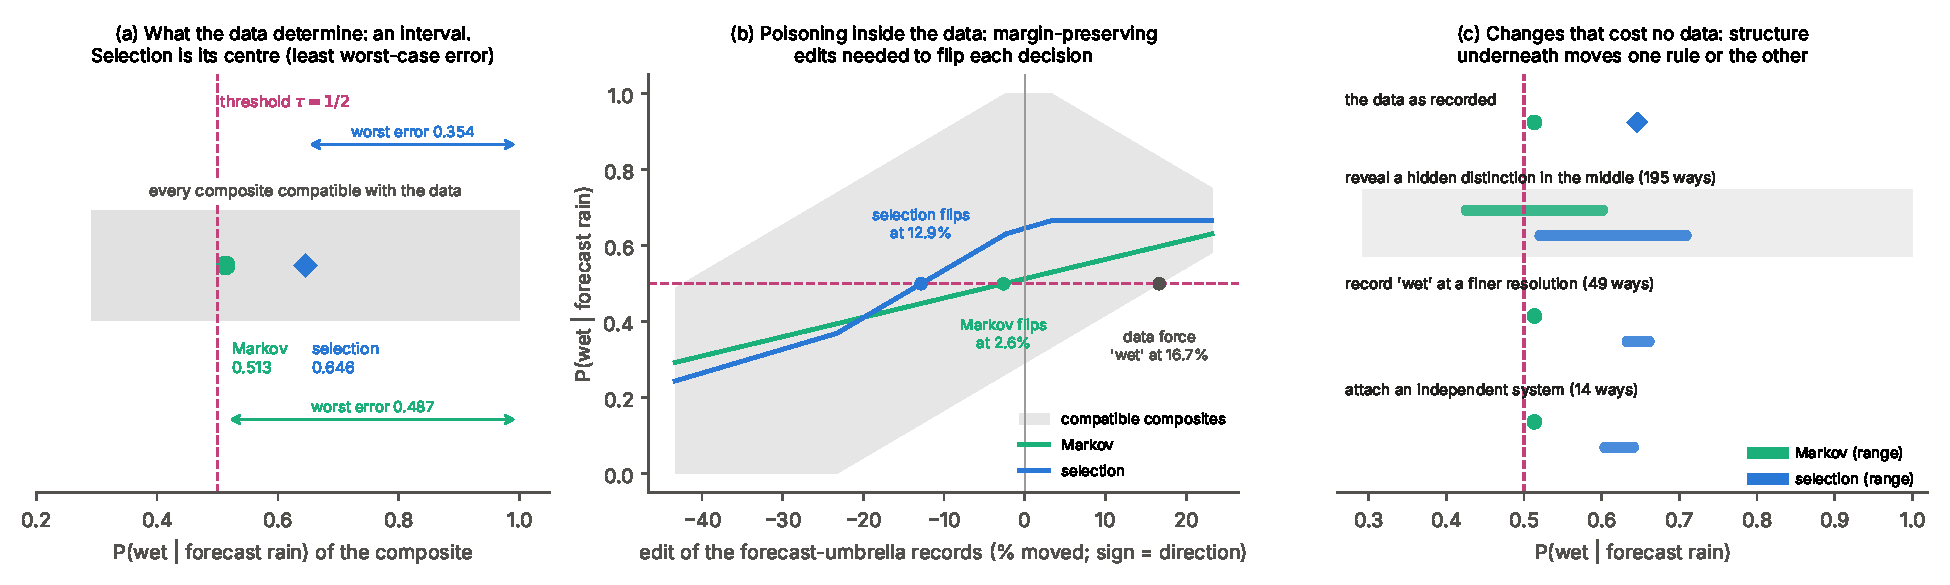
\includegraphics[width=\linewidth]{fig_selrob.pdf}
\caption{How little changes the decision in \cref{ex:umbrella}. (a) What the data determine: the identified interval (grey), the two composites, and their worst-case errors; selection sits at the centre. (b) Margin-preserving
edits of the forecast--umbrella records: Markov stops warning at $2.6\%$, selection at $12.9\%$, and the data themselves force a warning only at $16.7\%$. (c) Changes that cost no data. A hidden distinction in the middle
moves Markov across the threshold and shrinks the interval; a finer record of ``wet'' and an independent system move selection only.}\label{fig:selrob}
\end{figure}

\subsection{Selection as a section of the marginal projection}\label{sec:section}
\Cref{sec:probcat,sec:howlittle} compared two rules on chains. Both have the same shape: from local data, choose one joint law that agrees with the data. This subsection makes that shape the object of study. A rule is a section of a projection. Which laws such a rule obeys is a separate question, and a category appears only after a further step.

\paragraph{The projection.} Let $V$ be a finite set of variables with finite state sets $X_v$, and let $\mathcal C$ be a cover of $V$ by contexts $C\subseteq V$. Let $\mathcal J=\Delta(\prod_vX_v)$ be the simplex of joint laws, and
\[
\pi:\mathcal J\longrightarrow\textstyle\prod_{C\in\mathcal C}\Delta(X_C)
\]
the map to the family of context marginals. Write $\mathcal L$ for the locally consistent families, those whose marginals agree on overlaps, and $\mathcal D=\pi(\mathcal J)\subseteq\mathcal L$ for the data that some joint law produces. The fibre over $d\in\mathcal D$ is $\mathcal J_d=\pi^{-1}(d)$, and the points of $\mathcal L\setminus\mathcal D$ are the contextual data \cite{AbramskyBrandenburger2011}. A chain $X_0,\dots,X_n$ with contexts $\{X_{k-1},X_k\}$ is the case of \cref{sec:selcomp}, and there $\mathcal L=\mathcal D$ \cite{Vorobev1962}.

\begin{definition}[sections and their laws]\label{def:section}
A \emph{section} is a map $s:\mathcal D\to\mathcal J$ with $\pi\circ s=\mathrm{id}_{\mathcal D}$. Let $\Gamma$ be the group generated by relabelling states and by permutations of $V$ that preserve $\mathcal C$; it acts on $\mathcal J$ and on $\mathcal D$, and $\pi$ commutes with it. A section is \emph{equivariant} if $s(\gamma d)=\gamma s(d)$ for $\gamma\in\Gamma$; \emph{interior} if $s(d)$ lies in the relative interior of $\mathcal J_d$; \emph{system independent} if it sends the product data of two independent systems to the product of their sections; and \emph{natural} for a map $f:X_v\to X'_v$ if pushing the data forward along $f$ and then taking the section gives the pushforward of the section.
\end{definition}

The projection records which joint laws are compatible with the data. A section chooses one of them. Continuity, symmetry, system independence and naturality are further properties of that choice, and the projection implies none of them.

\begin{theorem}[the projection]\label{thm:projection}
\begin{enumerate}
\item[(1)] $\mathcal D$ is the convex hull of the images of the deterministic laws $\delta_\omega$, $\omega\in\prod_vX_v$. For $d\in\mathcal D$ the fibre $\mathcal J_d$ is a non-empty polytope; for $d\in\mathcal L\setminus\mathcal D$ there is no compatible joint law.
\item[(2)] For a face $G$ of $\mathcal D$ let $\Omega(G)=\{\omega:\pi(\delta_\omega)\in G\}$. Then $\pi^{-1}(G)$ is the face of $\mathcal J$ spanned by $\{\delta_\omega:\omega\in\Omega(G)\}$, and for $d$ in the relative interior of $G$
\[
\dim\mathcal J_d=|\Omega(G)|-1-\dim G.
\]
So the fibre is a single point over the whole of $G$ exactly when $|\Omega(G)|=\dim G+1$.
\item[(3)] $d\mapsto\mathcal J_d$ is Lipschitz in the Hausdorff metric on $\mathcal D$.
\end{enumerate}
\end{theorem}

\begin{proof}
(1) $\pi$ is linear and $\mathcal J$ is the simplex on the $\delta_\omega$. (2) Write $G=\mathcal D\cap\{\ell=0\}$ with $\ell$ affine and $\ell\ge0$ on $\mathcal D$. Then $\ell\circ\pi$ is affine and $\ge0$ on the simplex, so its zero set is the face spanned by the vertices where it vanishes, which are the $\delta_\omega$ with $\omega\in\Omega(G)$. That face is a simplex of dimension $|\Omega(G)|-1$, and $\pi$ maps it affinely onto $G$. The fibre of an affine surjection of polytopes over a relative-interior point has dimension equal to the difference of the dimensions; fibres of linear projections of polytopes are the subject of \cite{BilleraSturmfels1992}. (3) The fibres are the polyhedra $\{x\ge0:Ax=b(d)\}$ with fixed $A$, and these depend Lipschitz-continuously on $b$ on the set where they are non-empty \cite{WalkupWets1969}.
\end{proof}

\begin{theorem}[sections]\label{thm:sections}
\begin{enumerate}
\item[(1)] Every continuous, strictly concave $\phi$ on $\mathcal J$ gives a section $s_\phi(d)=\arg\max_{\mathcal J_d}\phi$, continuous on $\mathcal D$. For the entropy $H$ the section $s_H$ is continuous, interior, equivariant and system independent.
\item[(2)] The leximin section $s_{\mathrm{lex}}$ (\cref{def:lex} applied to $\mathcal J_d$, with the cell values as slacks) is equivariant wherever it is defined. It is not system independent.
\item[(3)] If the stabiliser $\Gamma_d$ of $d$ fixes exactly one point of $\mathcal J_d$, every equivariant section takes that value at $d$.
\end{enumerate}
\end{theorem}

\begin{proof}
(1) By \cref{thm:projection}(3) and Berge's maximum theorem the set of maximisers depends upper-semicontinuously on $d$; it is a single point, so it is continuous. The entropy has infinite slope into the interior at the boundary of a face, so its maximiser is relatively interior. $H$ is invariant under permutations of cells, and $\Gamma$ acts by permuting cells and maps $\mathcal J_d$ to $\mathcal J_{\gamma d}$, which gives equivariance. System independence is subadditivity, as in \cref{sec:probcat}: $H(x)\le H(x_1)+H(x_2)$ for a joint law of two systems with marginals $x_1,x_2$, with equality at the product. (2) Equivariance is the argument of \cref{prop:selkeeps}(3)--(4): a cell permutation preserves the facets and every step of the recursion. \Cref{prop:selbreaks}(1) is a counterexample to system independence. (3) $s(d)=s(\gamma d)=\gamma s(d)$ for $\gamma\in\Gamma_d$, so $s(d)$ is the fixed point.
\end{proof}

\begin{theorem}[from sections to a category]\label{thm:sec2cat}
On chain covers, let $S=(S_n)_{n\ge1}$ choose a section for every chain of every length, and set $\gamma_1\circ_S\gamma_2=$ the $(X_0,X_2)$ marginal of $S_2(\gamma_1,\gamma_2)$.
\begin{enumerate}
\item[(1)] $\circ_S$ is closed and unital, since the fibre over $(\gamma,D_q)$ is one point.
\item[(2)] Call $S$ \emph{inner-face consistent} if, for every $n\ge3$ and $0<i<n$, summing $X_i$ out of $S_n(\gamma_1,\dots,\gamma_n)$ gives $S_{n-1}(\gamma_1,\dots,\gamma_i\circ_S\gamma_{i+1},\dots,\gamma_n)$. Then $\circ_S$ is associative, and every bracketing of a chain equals the end marginal of $S_n$. So finite probability spaces, couplings and $\circ_S$ form a category.
\item[(3)] If moreover $S$ is equivariant (reversal included), system independent, or natural for end maps, the category is respectively a dagger category, monoidal, or compatible with coarse-graining the ends.
\item[(4)] Maximum entropy is inner-face consistent, and its category is $\mathsf{Cpl}$ with Markov gluing. The leximin family is not inner-face consistent.
\end{enumerate}
\end{theorem}

\begin{proof}
(2) Both bracketings of $(\gamma_1,\gamma_2,\gamma_3)$ are end marginals of faces of $S_3$: summing out $X_2$ gives $S_2(\gamma_1,\gamma_2\circ\gamma_3)$, and summing out $X_1$ gives $S_2(\gamma_1\circ\gamma_2,\gamma_3)$. Both therefore equal the end marginal of $S_3$, and induction on $n$ handles longer chains. (3) The three properties pass to end marginals. (4) The maximum-entropy law with given consecutive marginals is the Markov chain, and summing out an inner variable of a Markov chain gives the Markov chain of the composed kernel. For leximin, \cref{thm:k4} gives a top composite that differs from a bracketing; MS2 checks both statements.
\end{proof}

Inner-face consistency is sufficient for associativity; we do not claim it is necessary. In the language of the table in \cref{sec:probcat}, each law of a composition is a property of the section family: units are a property of the one-point fibres; dagger and relabelling are equivariance; the tensor square is system independence; coarse-graining is naturality; and associativity is coherence under marginalisation across different decompositions of a chain.

\begin{problem}[the associative-section problem]\label{prob:assocsec}
Characterise the section families on chain covers that are unital, equivariant under relabelling and reversal, system independent, and inner-face consistent. Is maximum entropy the only one? Or do other associative families exist, with or without system independence?
\end{problem}

\Cref{thm:sec2cat} gives a sufficient mechanism. It does not say that every associative composition arises from an inner-face consistent family, nor that maximum entropy is the only such family. Shore and Johnson's theorem (\cref{rem:shorejohnson}) does not settle \cref{prob:assocsec} either, because its axioms quantify over a different class of rules. Leximin shows that equivariance and units do not imply coherence.

\begin{remark}[associativity as a Beck--Chevalley condition; symmetry as a topos quotient]\label{rem:beckchevalley}
Inner-face consistency asks that forgetting an inner variable commute with the chosen gluing. In the categorical treatment of Markov kernels, composition is exactly gluing followed by marginalisation of the middle variable \cite[\S\S11--13]{Fritz2020}. That this composition is associative rests on the Markov property, which makes the relevant squares of pushforwards and pullbacks commute. We read that as a condition of Beck--Chevalley type. \Cref{thm:sec2cat}(4) is that statement for the maximum-entropy section. The selection associator of \cref{sec:selbin} and the configuration of \cref{thm:k4} measure the failure of the same condition for the leximin section. The associativity failures are therefore failures of a Beck--Chevalley condition for a gluing that is not Markov; they do not come from the geometry of the spaces involved. Hyperconnected geometric morphisms do not account for them: geometric morphisms compose associatively, and a map of finite state spaces induces a localic morphism, whose hyperconnected part is trivial. Where topos theory does enter is symmetry. Equivariance of sections (\cref{thm:sections}(3)) is a statement about $\Gamma$-sets, and hyperconnected quotients of a topos correspond to such actions \cite{Hora2023}. We claim no more than this dictionary.
\end{remark} \Cref{thm:sec2cat} also says where the selection associator of \cref{sec:selbin} comes from: it measures the failure of the leximin family to be inner-face consistent.

\begin{remark}[maximum entropy, with care]\label{rem:shorejohnson}
Shore and Johnson \cite{ShoreJohnson1980} derive minimum relative entropy as the only updating rule satisfying four consistency axioms: uniqueness, invariance, system independence and subset independence. Their axioms quantify over all linear constraint sets on all finite spaces, and their reading has been debated \cite{Uffink1995}. Our sections are defined only on the fibres of one projection, so their theorem does not make maximum entropy the unique section with any particular list of the properties above. We therefore prove each law directly. The comparison table of \cref{sec:probcat} shows which laws separate the two rules; system independence is one of them.
\end{remark}

\begin{remark}[three layers]\label{rem:layers}
The sheaf-theoretic approach to contextuality \cite{AbramskyBrandenburger2011,AbramskyMansfieldBarbosa2012} asks whether compatible local data have a global probabilistic extension. Here a global section of the event sheaf is a \emph{deterministic} assignment, and our fibre $\mathcal J_d$ is the polytope of probability distributions over those assignments: its vertices are exactly the deterministic global sections. In that language \cref{thm:projection}(2) says that over a face $G$ the data can use exactly the deterministic global sections in $\Omega(G)$, and that the mixture of them is pinned down exactly when they are affinely independent; \cref{cor:rigid,thm:ncycle} say this happens along the whole contextuality boundary of every cycle. We study the geometry of the space of extensions and the rules that choose among them. Information cohomology \cite{BaudotBennequin2015,Vigneaux2020} gives a complementary perspective on the identities that particular rules satisfy, maximum entropy above all. The three study different objects: the event sheaf, convex fibres of global distributions and their sections, and information structures with coefficient modules. The bridge between them is constructed here only as far as \cref{prop:cocycle}.

The two sheaf axioms give a short dictionary. \emph{Gluing}, the existence of a global section, is $\mathcal J_d\neq\varnothing$: no contextuality. \emph{Locality}, the uniqueness of the glued section, is $\dim\mathcal J_d=0$: the data determine the joint law. Positivity is the only obstruction to gluing. If signed measures are allowed, every locally consistent family has a global extension \cite{AbramskyBrandenburger2011,AlSafiShort2013}, and these extensions form an affine space $\mathcal A_d=\{x:\pi(x)=d,\ \sum_\omega x_\omega=1\}$ whose dimension is the same for every $d\in\mathcal L$ (here $15-8=7$ for the 4-cycle). The linear layer, as for a fine sheaf, has no obstruction; the fibre is its intersection with the simplex, $\mathcal J_d=\mathcal A_d\cap\mathcal J$. Contextuality is $\mathcal A_d\cap\mathcal J=\varnothing$. \Cref{cor:rigid,thm:ncycle} say that at the contextuality boundary the affine space, of dimension $2^n-1-2n$ for the $n$-cycle, meets the simplex in a single point: where gluing is about to fail, the gluing is unique. How far $\mathcal A_d$ lies from the simplex is measured by the contextual fraction \cite{AbramskyBarbosaMansfield2017}, the largest weight of a global subprobability that fits under the data.
\end{remark}

\begin{proposition}[what the cocycle gives]\label{prop:cocycle}
In the settings of \cite{BaudotBennequin2015,Vigneaux2020} the degree-one information cocycles are the multiples $cH$ of Shannon entropy, and the cocycle condition is the chain rule $H(X,Y)=H(X)+H(Y\mid X)$. For a section defined by maximising $cH$ on each fibre:
\begin{enumerate}
\item[(1)] if $c>0$ the maximiser is unique and the section is system independent. This uses the identity $H(P\otimes P')=H(P)+H(P')$, which is the cocycle condition, together with the inequality $H(P_{XY})\le H(P_X)+H(P_Y)$, that is $I(X;Y)\ge0$, which is concavity and not cohomology;
\item[(2)] if $c<0$ the cocycle condition still holds, but the maximisers of $cH$ are the minimisers of $H$, which are attained at vertices and need not be unique, so no section is defined. For the binary chain with all marginals $1/2$ and $\gamma_1=\gamma_2=\left(\begin{smallmatrix}1/4&1/4\\1/4&1/4\end{smallmatrix}\right)$, the fibre is a square, and all four vertices have entropy $\log4$, the minimum.
\end{enumerate}
So the cocycle together with strict concavity gives system independence, and the cocycle alone does not.
\end{proposition}

\begin{proof}
(1) Strict concavity gives uniqueness; for system independence see the proof of \cref{thm:sections}(1). (2) A concave function on a polytope attains its minimum at a vertex. In the example, the flip $x\mapsto1/4-x$ in either slice maps the fibre to itself and preserves entropy, and it permutes the four vertices; each vertex has four cells equal to $1/4$ and four equal to $0$ (MS11).
\end{proof}

Concavity alone is not enough either. The Cressie--Read power family \cite{CressieRead1984}
\[
\phi_q(x)=\frac{x^q-x}{q(1-q)},\qquad q\le1,
\]
gives a strictly concave cell functional for each $q$. It is Shannon's $-x\log x$ at $q=1$ and Burg's $\log x$ at $q=0$, up to terms constant on a fibre, and it moves toward the leximin point as $q\to-\infty$. MS11 maximises $\sum_c\phi_q(x_c)$ on the fibres of the forecast--umbrella chain, of a second binary chain and of their product, and measures how far the product chain's section is from the product of the two sections, in total variation (numerical, $40$ digits):
\begin{center}\small
\begin{tabular}{lcccccccc}\toprule
$q$ & $1$ & $0.99$ & $0.9$ & $0.5$ & $0$ & $-1$ & $-4$ & $-8$\\
defect & $<10^{-15}$ & $0.0008$ & $0.0077$ & $0.032$ & $0.049$ & $0.064$ & $0.073$ & $0.075$\\\bottomrule
\end{tabular}
\end{center}
The facet-leximin selection has defect $0.0752$. Within this family only the Shannon member passes the tensor square, and the defect grows steadily toward the leximin value. That is what Shore and Johnson's system-independence axiom predicts for separable functionals \cite{ShoreJohnson1980}. Here it is a computation on one pair of chains, not a proof of \cref{prob:assocsec}; \cref{fig:sections} draws it.

\begin{figure}[!htbp]\centering
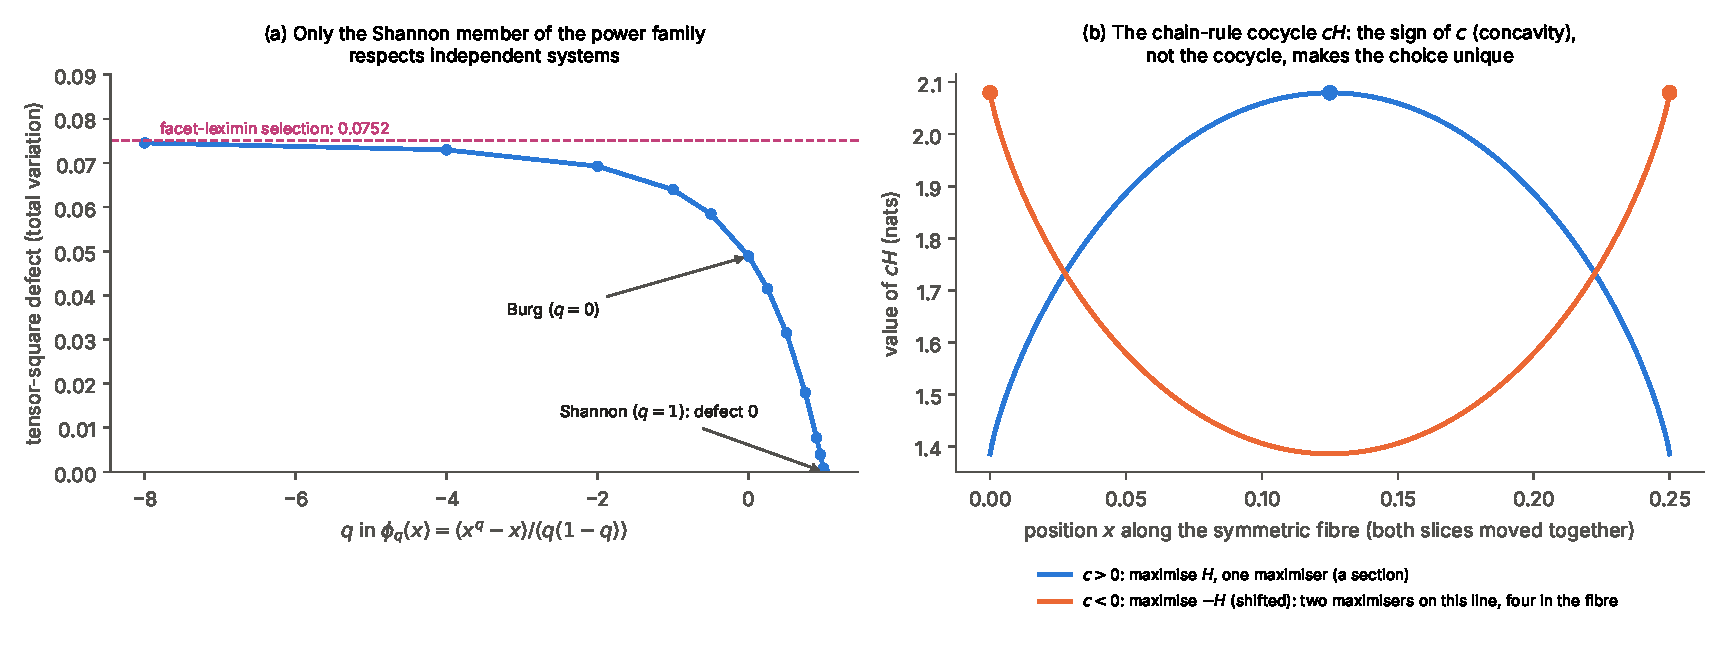
\includegraphics[width=\linewidth]{fig_sections.pdf}
\caption{(a) The tensor-square defect of the section that maximises $\sum_c\phi_q(x_c)$: zero only at Shannon ($q=1$), rising toward the facet-leximin value. (b) The chain-rule cocycle $cH$ on a symmetric fibre: for $c>0$ it has one maximiser, for $c<0$ several (four in the fibre). Uniqueness comes from the sign of $c$, that is from concavity, not from the cocycle.}\label{fig:sections}
\end{figure}

\subsection{The 4-cycle cover}\label{sec:cycle}
The smallest cover with a cycle has four binary variables $A_0,A_1,B_0,B_1$ and contexts $\{A_i,B_j\}$: the cycle $A_0-B_0-A_1-B_1-A_0$ of the CHSH setting. Data are four $2\times2$ tables that agree on the single marginals. They are coordinatised by eight numbers, the four entries $P(A_i=0,B_j=0)$ and the four probabilities $P(A_i=0)$, $P(B_j=0)$. Then $\mathcal J$ is the simplex on $16$ outcomes, of dimension $15$, $\mathcal D$ has dimension $8$, and the generic fibre has dimension $7$.

\begin{proposition}[the marginal polytope of the 4-cycle]\label{prop:cycleD}
$\mathcal D$ has $16$ vertices, the images of the deterministic laws, and exactly $24$ facets. Sixteen of them are the local inequalities of $\mathcal L$, the nonnegativity of the sixteen table entries. The other eight are the Clauser--Horne inequalities \cite{ClauserHorne1974}, for example
\[
P(A_0B_0)+P(A_0B_1)+P(A_1B_0)-P(A_1B_1)\ \le\ P(A_0)+P(B_0),
\]
where $P(A_iB_j)$ stands for $P(A_i=0,B_j=0)$ and $P(A_0)$ for $P(A_0=0)$; the others are obtained by choosing which context carries the minus sign and by the four with $\ge -1$ in place of $\le 0$. So $\mathcal D=\mathcal L\cap\{\mathrm{CH}\}$, which is Fine's theorem \cite{Fine1982}. On the symmetric path with uniform marginals and correlations $\lambda,\lambda,\lambda,-\lambda$, whose CHSH value is $S=4\lambda$, the data lie in $\mathcal L$ for $\lambda\le1$ and in $\mathcal D$ exactly for $\lambda\le1/2$. Past $S=2$ there is no joint law, up to the PR box at $\lambda=1$.
\end{proposition}

\begin{proof}
Exact enumeration: every hyperplane through eight affinely independent vertices that has all sixteen vertices on one side (MS3); MS5 checks the path.
\end{proof}

\begin{proposition}[fibres over the boundary]\label{prop:cyclefibres}
$\mathcal D$ has $2721$ faces. By \cref{thm:projection}(2) the fibre dimension over the interior of a face $G$ is $|V(G)|-1-\dim G$, and the counts are:
\begin{enumerate}
\item[(1)] the interior: fibre dimension $7$;
\item[(2)] the $16$ positivity facets, each with $12$ vertices: fibre dimension $4$. A structural zero leaves a four-parameter family of joint laws;
\item[(3)] the $8$ Clauser--Horne facets, each with $8$ vertices: these are $7$-simplices, so every point of a closed CH facet, including all $1752$ faces lying in CH facets, has exactly one compatible joint law;
\item[(4)] the remaining lower faces, where the fibre dimension is $0$ on $400$ further faces and $1$, $2$ or $3$ on the others (\cref{fig:cycle}(a)).
\end{enumerate}
\end{proposition}

\begin{proof}
Exact face enumeration (MS4), checked against the numerical fibre dimension at an interior point of $40$ sampled faces.
\end{proof}

So the collapse of the fibre at the boundary of $\mathcal D$ is a fact to be proved, not a consequence of being on the boundary. It holds at the CH facets because each is a simplex, and it fails at the positivity facets. Those facets are facets of $\mathcal L$ as well: crossing them makes a table entry negative, not the data contextual. The contextuality boundary is the part of $\partial\mathcal D$ that lies in the relative interior of $\mathcal L$, and it consists of points of CH facets.

\begin{corollary}[the contextuality boundary is rigid]\label{cor:rigid}
For the 4-cycle, every point of $\partial\mathcal D$ that is not on a positivity facet has exactly one compatible joint law. Ambiguity at the boundary of $\mathcal D$ survives only at structural zeros.
\end{corollary}

\begin{proof}
Such a point lies on a facet of $\mathcal D$ that is not a positivity facet, hence on a CH facet, and \cref{prop:cyclefibres}(3) applies.
\end{proof}

That a CHSH facet carries eight deterministic points is a direct count (\cref{thm:ncycle}(1) with $n=4$). The consequence for identification, that a unique joint law exists along the whole contextuality boundary, follows at once; we have not found it stated in this form. \Cref{sec:ncycle} shows that it holds for every cycle.

\subsection{At the contextuality boundary: sections and robustness}\label{sec:cycleboundary}
Fibre collapse and agreement of the sections are different questions, so we track them separately.

\begin{proposition}[the symmetric path]\label{prop:chshpath}
On the symmetric path the stabiliser of the data, among the automorphisms of the 4-cycle combined with bit flips, contains a group of order $16$ (all of it for $\lambda=2/5$), and the fixed set of that group in the fibre is a single point for every $\lambda\in[0,1/2]$. By \cref{thm:sections}(3) every equivariant section therefore takes the same value; maximum entropy and leximin agree. The unobserved quantity $q=P(A_0=0,A_1=0)$, whose variables are never measured together, has identified interval $[\lambda/2,\,(1-\lambda)/2]$. Its width $(2-S)/4$ goes to $0$ at the CH facet, where the single joint law gives $q=1/4$.
\end{proposition}

\begin{proof}
The fixed equations together with the fibre equations have rank $16$ and do not depend on $\lambda$ (MS6, exact). The interval is computed by linear programming at $21$ values of $\lambda$, to $10^{-9}$ (numerical).
\end{proof}

Without symmetry the two sections disagree, and the question becomes whether the disagreement survives at the boundary. MS7 follows straight paths from one interior point to a generic point of three kinds of face (numerical):

\begin{center}\small
\begin{tabular}{lcccc}\toprule
toward & \multicolumn{2}{c}{fibre width (largest range of a cell)} & \multicolumn{2}{c}{disagreement $\tfrac12\|s_H-s_{\mathrm{lex}}\|_1$}\\
& at $0.9$ & at the face & at $0.9$ & at the face\\\midrule
a CH facet & $0.051$ & $0$ & $0.053$ & $0$\\
a positivity facet & $0.377$ & $0.364$ (fibre $4$) & $0.048$ & $0.051$\\
a $6$-face with $10$ vertices & $0.302$ & $0.320$ (fibre $3$) & $0.025$ & $0.034$\\\bottomrule
\end{tabular}
\end{center}

The disagreement of any two sections is at most $8$ times the fibre width, since $\tfrac12\|x-y\|_1\le\tfrac12\cdot16\max_c|x_c-y_c|$. So the sections are forced together exactly as fast as the fibre closes, and only where it closes. As the data approach a CH facet every rule gives nearly the same joint law, and the identified set of every unobserved quantity shrinks with the fibre. A rule then cannot be steered without moving the data. At a structural zero the data still allow a four-parameter family, so rules disagree and decisions depend on the rule, as in \cref{sec:howlittle}. One step past the CH facet no joint law is left, and every section fails at once. In this sense the contextuality boundary is where marginal data come closest to determining the joint law, immediately before they become inconsistent with every joint law.

\subsection{Simpson's reversal in the same framework}\label{sec:simpson}
A chain cover never records all three variables together, so the sign of an association between the ends given the middle is not in the data. It is chosen by the section.

\begin{proposition}[Simpson's reversal]\label{prop:simpson}
\begin{enumerate}
\item[(1)] \emph{Selection sensitivity: made by the rule.} For $\gamma_1=\left(\begin{smallmatrix}5/24&11/24\\1/24&7/24\end{smallmatrix}\right)$ and $\gamma_2=\left(\begin{smallmatrix}3/23&11/92\\15/22&3/44\end{smallmatrix}\right)$, the selected joint law has conditional covariance of $(X_0,X_2)$ equal to $1/276$ given $X_1=0$ and $1/99$ given $X_1=1$, but marginal covariance $-31/4048$: a Simpson reversal \cite{Simpson1951}. The Markov section has conditional covariance $0$ in both slices and marginal $-49/3036$. The compatible marginal covariances fill $[-95/1518,\,287/6072]$, and at the upper end the conditional covariances are $\ge0$ as well, so the same data admit a joint law with no reversal.
\item[(2)] \emph{Information-loss sensitivity: made by coarse-graining the middle.} For $\gamma_1=\left(\begin{smallmatrix}4/21&3/14&2/21\\1/7&2/21&11/42\end{smallmatrix}\right)$ and $\gamma_2=\left(\begin{smallmatrix}1/9&2/9\\65/252&13/252\\5/32&45/224\end{smallmatrix}\right)$, Markov gluing gives marginal covariance $85/4032>0$ with three middle states and $-43/6272<0$ after merging the last two. Selection goes from $13/448$ to $-1/42$.
\end{enumerate}
\end{proposition}

\begin{proof}
Exact computation (MS8, MS9).
\end{proof}

The two mechanisms differ. In (1) the data leave the joint law underdetermined, and the reversal comes from how a rule completes it; Markov gluing is not neutral either, since setting the conditional association to zero is also a completion. In (2) the reversal comes from forgetting a distinction in the conditioning variable, which is the classical aggregation form of Simpson's paradox. The first is a sensitivity to the choice of section, the second a sensitivity to information loss, and the framework keeps them apart.

\paragraph{What the sections support.} Taking \crefrange{sec:section}{sec:simpson} together:
\begin{enumerate}
\item[(1)] The projection alone sorts the data: empty fibre (contextual), a point (determined), or a positive-dimensional polytope (identified up to a set).
\item[(2)] A section is a rule. On chains, maximum entropy is inner-face consistent and gives the dagger symmetric monoidal category $\mathsf{Cpl}$. Leximin keeps the symmetries but gives no category.
\item[(3)] On the 4-cycle, composition is not the question. What survives is the section and its symmetry, and contextual data have no section at all.
\end{enumerate}
Simpson's reversal and the sign of a composed association are properties of the section or of the resolution of the middle, not of the recorded data. These are the precise forms of the statements that motivated this part. The underlying category is standard, and the new content is the section viewpoint with its exact compatibility and failure results.

\begin{figure}[!htbp]\centering
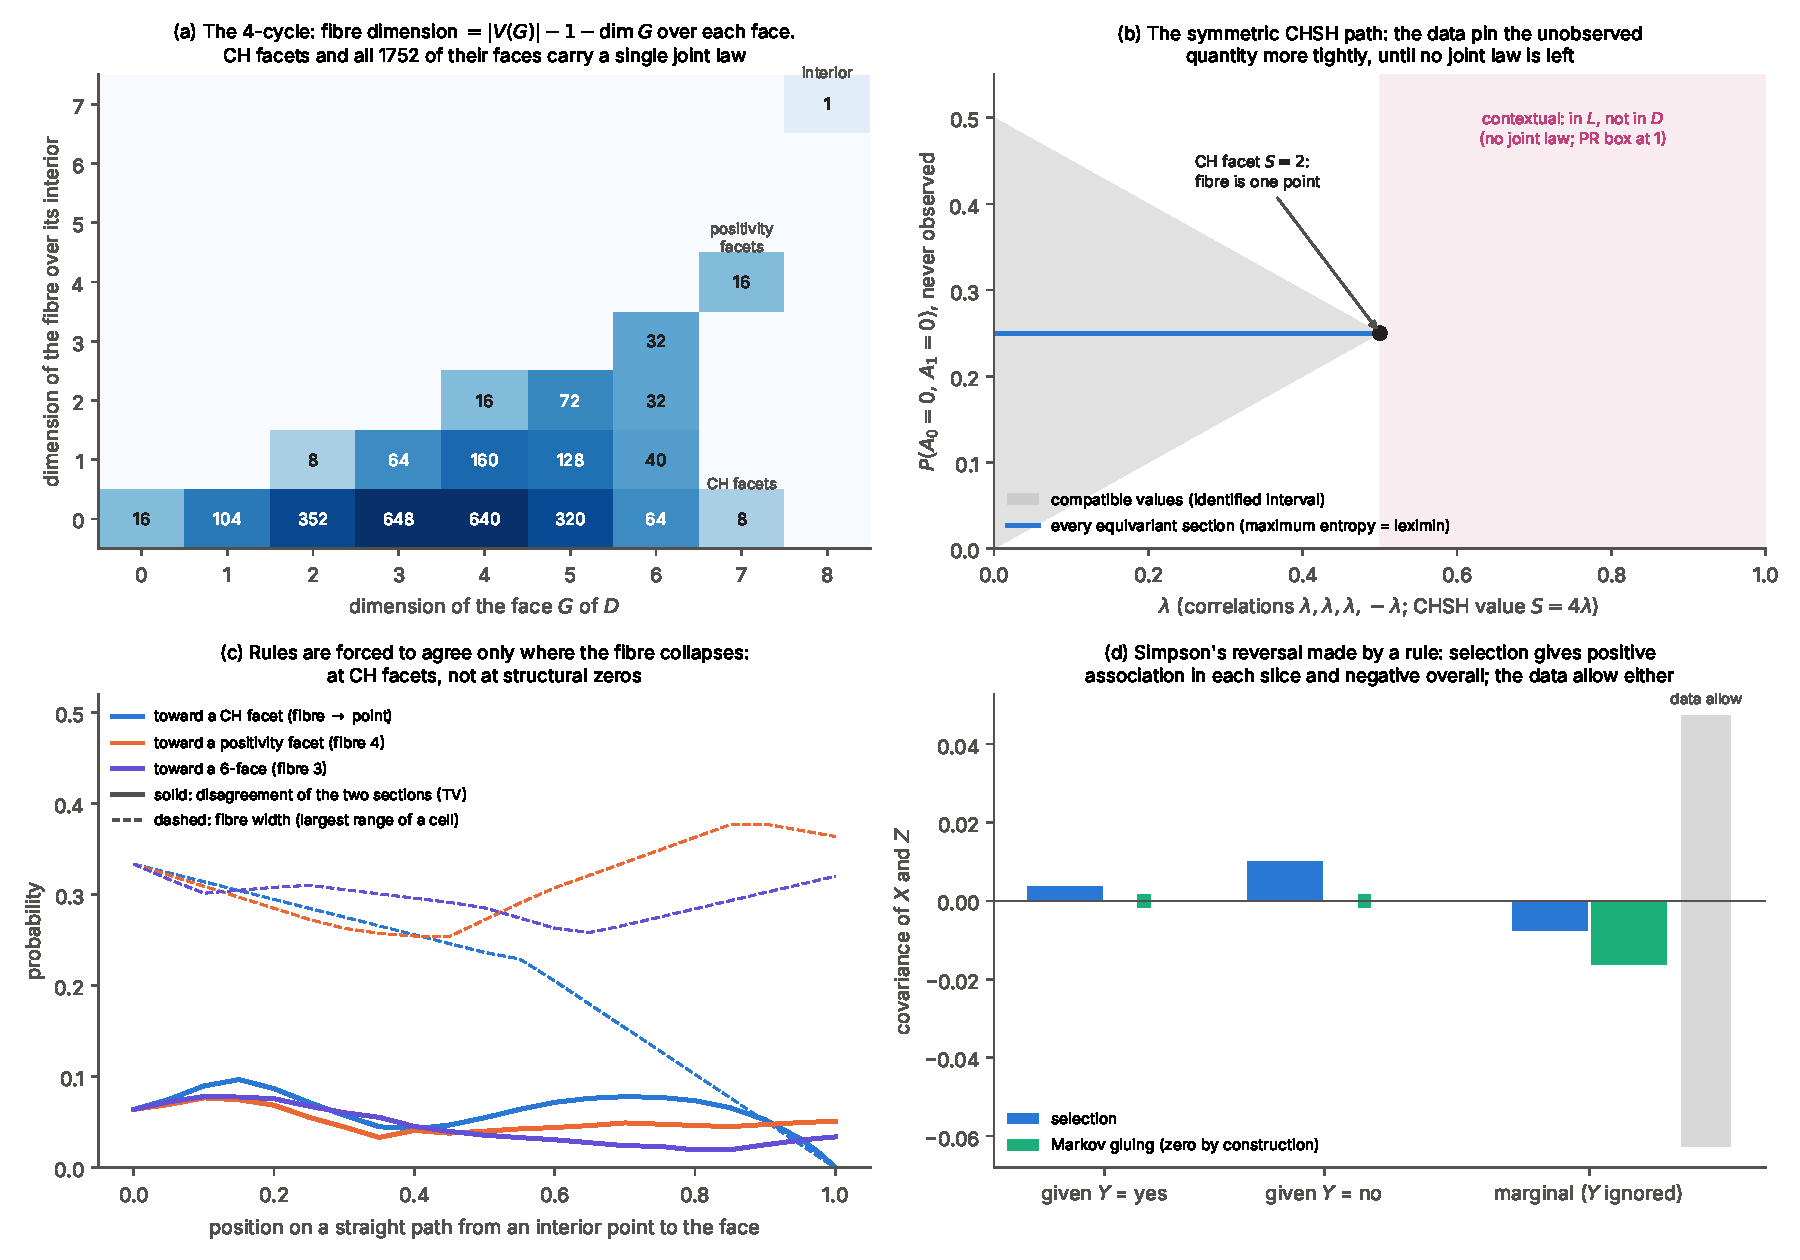
\includegraphics[width=\linewidth]{fig_cycle.pdf}
\caption{The 4-cycle and Simpson. (a) Faces of the marginal polytope $\mathcal D$ by dimension, against the dimension of the fibre over their interior. The Clauser--Horne facets are simplices, so there the data determine the joint law; positivity facets leave a four-dimensional fibre. (b) The symmetric CHSH path: the identified interval of the never-observed $P(A_0=0,A_1=0)$ closes at $S=2$, where every equivariant section is forced to $1/4$, and past it the data are contextual. (c) Straight paths to three kinds of face: the two sections disagree until the fibre closes, and only a CH facet closes it. (d) A Simpson reversal made by selection: positive association within each slice of $X_1$ and negative overall. Markov gluing has zero association within the slices, and the data allow either sign overall.}\label{fig:cycle}
\end{figure}

\subsection{Every cycle: the contextuality boundary is a union of simplices}\label{sec:ncycle}
The $n$-cycle cover has binary variables $X_0,\dots,X_{n-1}$ and contexts $\{X_i,X_{i+1}\}$, indices mod $n$; $n=4$ is the CHSH case and $n=5$ the KCBS case. Data are the $n$ entries $P(X_i=0,X_{i+1}=0)$ and the $n$ singles, so $\dim\mathcal D=2n$, and the generic fibre has dimension $2^n-1-2n$. For $n\ge4$, Ara\'ujo et al.\ \cite{AraujoEtAl2013} show that the facets of $\mathcal D$ are the $4n$ local inequalities and the $2^{n-1}$ noncontextuality inequalities
\[
\textstyle\sum_{i}\gamma_i\langle X_iX_{i+1}\rangle\ \le\ n-2,\qquad\gamma_i\in\{\pm1\},\ \ \prod_i\gamma_i=-1,
\]
in $\pm1$ notation, where $\langle X_iX_{i+1}\rangle=1-2P(X_i\ne X_{i+1})$ is linear in the data. For $n=3$ our exact enumeration gives the same list.

\begin{theorem}[rigidity of the contextuality boundary for every cycle]\label{thm:ncycle}
For every $n\ge3$:
\begin{enumerate}
\item[(1)] each noncontextuality facet of $\mathcal D$ contains exactly $2n$ deterministic points and is a $(2n-1)$-simplex. So every point of the contextuality boundary, the part of $\partial\mathcal D$ in the relative interior of $\mathcal L$, has exactly one compatible joint law;
\item[(2)] each local facet contains $3\cdot2^{n-2}$ deterministic points, so the fibre over its interior has dimension $3\cdot2^{n-2}-2n$; this is $4$ for $n=4$, $14$ for $n=5$ and $36$ for $n=6$.
\end{enumerate}
\end{theorem}

\begin{proof}
(1) A deterministic assignment $x\in\{\pm1\}^n$ has edge values $e_i=x_ix_{i+1}$ with $\prod_ie_i=1$, and $\sum_i\gamma_ie_i=n-2k$, where $k$ counts the edges with $e_i\ne\gamma_i$. Since $\prod\gamma_i=-1$, $k$ is odd, so the inequality holds, with equality exactly when $k=1$. Choosing the one edge where $e_i\ne\gamma_i$ ($n$ ways) fixes every $e_i$, and $x$ is then fixed up to a global flip ($2$ ways): $2n$ points. They span a facet, of dimension $2n-1$, so they are affinely independent, and the facet is a simplex. \Cref{thm:projection}(2) then gives a one-point fibre over every point of it, its faces included. (2) The local facet $P(X_i=a,X_{i+1}=b)\ge0$ contains the assignments that avoid the pair $(a,b)$ on that edge, which are three quarters of the $2^n$. Apply \cref{thm:projection}(2) with $\dim G=2n-1$.
\end{proof}

MS10 recomputes all facets of $\mathcal D$ exactly for $n=3,4,5$, independently of \cite{AraujoEtAl2013}: $16$, $24$ and $36$ facets, the counts $4n+2^{n-1}$, with the vertex numbers above and the noncontextuality facets in exactly the $\gamma$ form. For $n=6,7,8$ it checks that every listed inequality is valid and a facet with the stated vertex count. Completeness of the list there is taken from \cite{AraujoEtAl2013}. So the rigidity found for CHSH is not special to the 4-cycle. On every cycle the contextuality boundary is a union of simplices, and the data there determine the joint law. The ambiguity left at a structural zero grows exponentially in $n$, while the contextuality boundary stays rigid. Whether the noncontextuality facets of other scenarios are simplices is a separate question that we have not tested. Where they are not, \cref{thm:projection}(2) measures how much ambiguity survives at the boundary.

\paragraph{Signs around the cycle.} The proof of \cref{thm:ncycle} rests on one observation. Around a cycle, the edge values of a deterministic assignment multiply to $+1$, while the noncontextuality inequalities are indexed by the sign patterns whose product is $-1$. The extreme case makes this a criterion. Give every single variable the uniform law and every edge a perfect correlation or anticorrelation.

\begin{proposition}[a twist around the cycle]\label{prop:twist}
Let $s\in\{\pm1\}^n$, and let $B_s$ be the $n$-cycle data with uniform singles and $\langle X_iX_{i+1}\rangle=s_i$ for every $i$.
\begin{enumerate}
\item[(1)] $B_s$ has a compatible joint law iff $\prod_is_i=+1$. If $\prod_is_i=-1$, no deterministic assignment is compatible with any part of $B_s$, so its noncontextual fraction is $0$.
\item[(2)] If one context is removed, so that the cover is a path, a compatible joint law exists for every $s$.
\end{enumerate}
\end{proposition}

\begin{proof}
A perfect correlation forces $x_ix_{i+1}=s_i$ on every assignment that carries weight, and these products multiply to $1$ around the cycle. So if $\prod s_i=-1$, no assignment can carry weight. If $\prod s_i=+1$, choose $x_0$, propagate $x_{i+1}=s_ix_i$, and mix the resulting assignment with its global flip at weight $\tfrac12$ each. On a path the propagation never closes up, so the same construction works for every $s$.
\end{proof}

The obstruction is a single sign carried around a closed loop, a twist, like the half-turn of a M\"obius band. A PR box is the $4$-cycle with the twist. The noncontextuality facets of \cref{thm:ncycle} are its fractional shadows. Each is indexed by a twisted sign pattern, and the data cross it when they correlate too strongly in the twisted pattern. The same sign drives the Kochen--Specker argument in Mermin's square: nine $\pm1$ observables whose row products are $+1$ and whose column products are $(+1,+1,-1)$ cannot all have values, since the product of the row products equals the product of the column products \cite{Mermin1990,Peres1990}. Heusler, Schlummer and Ubben trace the $-1$ in the quantum version to the difference between $IJK=-1$ and $JIK=+1$ for the spin flips $I,J,K$. The Bloch sphere cannot show this difference, because it forgets the overall sign of an $SU(2)$ element, and they recover it with Dirac's belt \cite{HeuslerSchlummerUbben2020}. Here the sign is classical, a property of the observed tables, but it plays the same role. It also explains a feature of \cref{ex:history}: local tables always glue along a path, and gluing can fail only when a cycle closes, because only a closed loop can carry a twist. ST1--ST3 confirm (1) and (2) for every sign pattern with $n\le7$, and the count of Mermin assignments.

\subsection{How little poisoning, in many dimensions}\label{sec:poisondim}
\Cref{sec:howlittle} measured edits of one binary chain. Here the cover is general, the decision concerns a quantity that is never observed, and three different things are counted: how many cells of the data an attacker must change, how much can change with no data edit at all, and how a change over time is explained afterwards.

\paragraph{Setting.} Data $d\in\mathcal D$ give the context tables, whose entries are affine in $d$: $Ed+e_0$, with $4n$ entries for the $n$-cycle. An edit $\delta$ costs $c(\delta)=\tfrac12\|E\delta\|_1$, the total variation summed over the context tables. When each context is a separate sample this is the fraction of records edited, summed over the samples, and on one table it is the $2|s|$ of \cref{prop:poison}. An edit is \emph{undetectable} when $d+\delta\in\mathcal D$. Then the tables still agree on shared margins and are noncontextual, so no margin check or contextuality test sees it. The undetectable directions lie in the \emph{consistent-edit space} $\Delta=\operatorname{range}E$, of dimension $\dim\mathcal D$ ($2n$ for the $n$-cycle). The decision is $w\cdot s(d)\ge\tau$ for a section $s$ and a quantity $w$ on joint laws whose variables are never observed together, here $P(X_0=X_2)$ on the $n$-cycle and $P(A_0=A_1)$ on CHSH. Write $[L(d),U(d)]$ for its identified interval.

\begin{definition}[flip costs]\label{def:flipcost}
For a decision with $w\cdot s(d)>\tau$: $c_{\rm some}(d)$ is the least cost of an undetectable edit after which $L\le\tau$ (some rule flips), $c_{\rm all}(d)$ the least cost after which $U\le\tau$ (every rule flips), and $c_s(d)$ the least cost after which $w\cdot s\le\tau$.
\end{definition}

\begin{proposition}[two thresholds]\label{prop:twothresh}
\begin{enumerate}
\item[(1)] $c_{\rm some}\le c_s\le c_{\rm all}$ for every section $s$. The same order holds for the first flipping time along any fixed direction.
\item[(2)] $c_{\rm some}$ is the value of one linear program: minimise $\tfrac12\|E(\pi x-d)\|_1$ over joint laws $x$ with $w\cdot x\le\tau$. The edited data $\pi x$ lie in $\mathcal D$ by construction. The set $\{U\le\tau\}$ is the union of the half-spaces $y\cdot d'+y_0\le\tau$ over the vertices $(y,y_0)$ of the dual polyhedron $\{\pi^{\!\top}y+y_0\mathbf 1\ge w\}$, so $c_{\rm all}$ is the least of finitely many linear programs.
\item[(3)] $c_{\rm some}(d)=0$ exactly when $L(d)\le\tau$. When the decision is not identified, a change of rule flips it with no change to the data.
\end{enumerate}
\end{proposition}

\begin{proof}
(1) $w\cdot s(d')\in[L(d'),U(d')]$ for every $d'$. (2) $U(d')=\max\{w\cdot x:\pi x=d',\,x\ge0,\,\mathbf 1\cdot x=1\}$ is, by linear-programming duality, the minimum of $y\cdot d'+y_0$ over the dual vertices. (3) follows from the definition. PF3 compares the costs at $80$ points, and the first flipping times for the maximum-entropy section along $18$ directions (numerical).
\end{proof}

A \emph{circuit} of $\Delta$ is a nonzero edit whose entry vector $E\delta$ has minimal support. Two vectors are \emph{conformal} when no coordinate has opposite signs in them. Every vector of a subspace is a conformal sum of at most $\dim\Delta$ circuits \cite{Rockafellar1969,MullerRegensburger2016}, and the cost is additive over a conformal sum.

\begin{proposition}[sparsity of undetectable flips]\label{prop:sparse}
\begin{enumerate}
\item[(1)] Some cheapest undetectable flip, for $c_{\rm some}$ or $c_{\rm all}$, is a conformal sum of at most $\min(a,\dim\Delta)$ circuits. Here $a$ is the number of constraints of the flip region (pieces of $\{L\le\tau\}$ or $\{U\le\tau\}$, and facets of $\mathcal D$) that are tight at it.
\item[(2)] For the $n$-cycle, $\Delta$ has $188$ circuits for $n=4$ (supports $4,6,8,9$, in numbers $20,32,72,64$) and $481$ for $n=5$ (supports $4,6,8,10,11$). Every support is at most $2n+1$. For $n=4,\dots,8$ there are exactly $5n$ circuits of support $4$: the $n$ margin-preserving swaps of \cref{prop:poison}, and $4n$ shifts of one single margin, each moving mass between two cells in each of the two tables that contain the variable.
\end{enumerate}
\end{proposition}

\begin{proof}
(1) Fix the sign pattern of a cheapest flip $\delta^*$. The edits in $\Delta$ with that pattern form a cone generated by the circuits conformal to it, and on that cone the cost is linear, $c(\sum\lambda_kC_k)=\sum\lambda_k c(C_k)$. Minimising it subject to the region's linear constraints is a linear program in $\lambda\ge0$, and it attains the value $c(\delta^*)$. A vertex solution has at most as many nonzero $\lambda_k$ as tight constraints, and any cheapest flip is a conformal sum of at most $\dim\Delta$ circuits by the result just cited. (2) Exact enumeration (PF1): every circuit is the kernel of $\dim\Delta-1$ independent rows of $E$, and each candidate is verified with integer arithmetic.
\end{proof}

How often a single circuit is enough is a numerical question (PF2). Take a gap of $0.01$ below $L$, and $30$ random interior data points for each $n$. One support-$4$ circuit is already a cheapest flip in $30/30$, $30/30$, $28/30$, $28/30$ and $24/29$ of the cases for $n=4,\dots,8$; for $n=8$ that is $4$ cells out of $32$. On the 4-cycle, vertex optima use one circuit in $37$ of $40$ cases at gap $0.01$, and one, two or three circuits in $19$, $16$ and $5$ cases at gap $0.05$. So the smallest poisoned footprint does not grow with the number of variables. It is four cells in two tables, or in one, and larger gaps need a few circuits because the flip region has corners. This complements the results for samples \cite{BroderickGiordanoMeager2020,SteinhardtKohLiang2017,MahloujifarEtAl2019}. Those count records or coordinates of the inputs. Here the count is of cells of a marginal table, and the undetectable edits form a structured subspace.

\paragraph{Placement and the hidden structure.} Let the hidden structure be the support $S$ of the true joint law, the set of readings that occur. The data then lie in the relative interior of the face $G(S)$ of $\mathcal D$, the smallest face containing $\pi(S)$. Let $\Pi(S)$ be the number of signed circuits along which a small step stays in $\mathcal D$. It is the same at every point of the relative interior, and it counts the places an attacker can start an undetectable edit.

\begin{proposition}[placement]\label{prop:placement}
\begin{enumerate}
\item[(1)] $S\subseteq S'$ implies $\Pi(S)\le\Pi(S')$. Simpler hidden structure leaves fewer undetectable placements.
\item[(2)] $\dim G+\dim(\text{fibre over }G)=|V(G)|-1$. The freedom of the hidden structure splits into room to move the data undetected (the face dimension) and room for the rule to move the answer at no data cost (the fibre dimension).
\item[(3)] On the 4-cycle, over all $2721$ faces: a vertex allows $13$ of the $376$ signed circuits, a CH facet $252$, a positivity facet $287$, and the interior all $376$. At fixed face dimension a larger fibre mostly gives more placements, for instance $165.4$, $170.0$ and $186.7$ on average for fibres $0$, $1$, $2$ at dimension $5$. The one exception is dimension $6$, where fibre $1$ averages $204.6$ against $207$ for fibre $0$.
\end{enumerate}
\end{proposition}

\begin{proof}
(1) $G(S)\subseteq G(S')$, so every facet containing $G(S')$ also contains $G(S)$, and the feasible directions at $G(S)$ are those at $G(S')$ cut by more inequalities. (2) is \cref{thm:projection}. (3) is an exact count with rational facet normals and integer circuits (PF4), with $0$ violations of (1) over all inclusions of faces.
\end{proof}

At matched sparsity the split matters. Among faces with $8$ readings, the rigid CH facets allow more undetectable placements ($252$) than faces with fibre $1$ (about $205$) or fibre $2$ (about $187$). Rigidity does not make placements scarce. It removes the free route: every flip must move the data. With a budget the decisive question is whether the decision is identified at the point (PF5). Take a gap $g=0.05$ below the true value, on the sparsity-matched faces of Study 18 and three interior points. Wherever the decision is identified (all CH and fibre-$1$ faces tested, and one fibre-$2$ face), the cheapest flip costs at least $g$, and at most $4$ single circuits achieve one within $1.5g$. Wherever it is not identified (the other two fibre-$2$ faces and the interior points), $c_{\rm some}=0$ along all $376$ placements, while $c_{\rm all}$ ranges from $0.14$ to $0.45$. A defender who reports $[L,U]$ instead of one rule's value forces the attacker to pay $c_{\rm all}$.

\paragraph{Over time: removal as a contravariant functor.} Decisions are recomputed as data arrive, so the hidden structure, the face and the interval all move. An \emph{information state} is a pair $(B,C)$: a set of batches and a set of observed contexts, ordered by inclusion. Its object $R(B,C)$ is the integer pooled tables of the contexts in $C$ over the batches in $B$. For $(B',C')\le(B,C)$ the \emph{removal map} $R(B,C)\to R(B',C')$ subtracts the counts of the batches in $B\setminus B'$ and forgets the contexts in $C\setminus C'$.

\begin{proposition}[removal]\label{prop:removal}
\begin{enumerate}
\item[(1)] Removal maps compose, and removing nothing is the identity, so $R$ is a functor from the opposite of the poset of information states to sets of tables. Removing batches and forgetting contexts commute.
\item[(2)] Forgetting contexts can only widen the identified interval: $C'\subseteq C$ implies $[L_C,U_C]\subseteq[L_{C'},U_{C'}]$. So the value of a context, the width it removes, is nonnegative.
\item[(3)] On a stationary stream with pooled clean data $d$, add one batch of $k$ undetectable units with data $p$. Then $d_t=(1-q_t)d+q_tp$ with $q_t=k/(N_t+k)$. Every rule is flipped exactly while $q_t\ge q^*$, where $q^*$ is the least crossing point $(\tau-y\cdot d-y_0)/(y\cdot(p-d))$ over the dual vertices with $y\cdot(p-d)<0$. So the flip lasts while $N_t\le k(1-q^*)/q^*$.
\end{enumerate}
\end{proposition}

\begin{proof}
(1) Subtraction of counts and deletion of coordinates compose and commute. (2) Fewer constraints give a larger fibre. (3) $U$ is a minimum of affine functions, so it is concave along the segment from $d$ to $p$. Its sublevel set there is an interval ending at $p$, and it starts at the first crossing of a dual-vertex function. PF6 checks (1) on $200$ random chains and squares with integer counts, PF7 checks (2) at every time and every sub-cover, and PF8 checks (3) at $30$ times (numerical).
\end{proof}

The removal maps answer why a decision changed. Compare the object at the later state with the objects obtained by removing one batch, or forgetting one context, at a time. The changes that revert the decision are the explanations. The exact comparison is cheap here. When it is not, a first-order estimate, the gradient of the decision value times the removed batch's contribution, ranks the candidates, as in the influence approach of \cite{BroderickGiordanoMeager2020}. An explanation need not be unique: near a threshold, removing a clean batch can also revert a decision.

\begin{example}[one poisoned batch]\label{ex:poisonstream}
Batches of $1200$ units, each reported in all four contexts of CHSH, decision $P(A_0=A_1)\ge0.45$ by maximum entropy (PF6--PF9, \cref{fig:poisonflip}). Until $t=5$ the world is the first CH-facet law of Study 18. Its interval has width $0$, so the decision is identified and robust. From $t=6$ the hidden structure changes to $0.8$ times that law plus $0.2$ uniform, the data move into the interior, and the interval opens. At $t=10$ an attacker adds the cheapest batch that flips every rule: $2298$ units, all of one reading, against $12000$ clean units ($q^*=0.161$). Every rule is flipped at $t=10$ only, but the maximum-entropy decision stays flipped for $t=10$ to $15$. At each of those times, removing the poisoned batch is the only single removal that reverts the decision. The first-order estimate of its effect is within $6\%$ of the exact change ($0.075$ against $0.072$ at $t=10$). At the last time, forgetting a context widens the interval by $0.295$ or $0.38$. The batch is consistent and noncontextual, so no marginal test detects it, but it consists of a single reading, and comparing the objects over time detects it at once.
\end{example}

\begin{remark}[reading a change cell by cell]\label{rem:cellattr}
The removal maps attribute a change to batches; conformal sums attribute it to cells. A change $\delta=d_t-d_{t-1}$ between consistent states lies in $\Delta$, so it is a conformal sum $\sum_k\lambda_kC_k$ of at most $\dim\Delta$ unit-cost circuits. Nothing cancels, so $c(\delta)=\sum_k\lambda_k$, and the first-order effect on the decision value $\phi$ splits the same way, $\nabla\phi\cdot\delta=\sum_k\lambda_k\,\nabla\phi\cdot C_k$. The decomposition is not unique. But the least share of $c(\delta)$ that any decomposition must put on circuits of more than four cells is an invariant of $\delta$, computed by one linear program; call it the \emph{coordination} of $\delta$. \Cref{fig:edittypes} shows each kind of circuit on the four CHSH tables. In \cref{ex:poisonstream} (PF10), the clean steps before the attack, including the change of hidden structure at $t=6$, have coordination $0$: they are sums of margin shifts and swaps. The poisoned step has coordination $0.659$, and removing the poisoned batch later has $0.652$. The clean steps after the attack have $0.393$, because each partly undoes the poison. The poisoned step's three largest contributions to the decision are a margin shift ($-0.025$), a $6$-cell circuit ($-0.022$) and a $9$-cell circuit ($-0.014$), out of a first-order total of $-0.067$. One example does not make coordination a detector. It shows what the conformal-sum theorem buys: an undetectable change has a canonical vocabulary of elementary edits, and its cost and its first-order effect are additive over them.
\end{remark}

\begin{figure}[!htbp]\centering
\includegraphics[width=\linewidth]{fig_edittypes.pdf}
\caption{The kinds of undetectable edit, and one change read as a sum of them. Each diagram shows the four tables of the CHSH cover on the sides of the cycle $A_0$--$B_0$--$A_1$--$B_1$ (rows: the $A$ variable; columns: the $B$ variable). A $+$ cell gains mass and a $-$ cell loses it. (a) A swap: four cells in one table, all margins fixed. (b) A margin shift: one single margin moves, by two cells in each of the two tables that contain it. (c)--(e) Circuits of $6$, $8$ and $9$ cells that coordinate three or four tables. (f) A detectable edit: one table alone, so the tables disagree on a shared margin. (g) The poisoned step of \cref{ex:poisonstream}, cell by cell. (h) Its conformal decomposition beside a clean step's: clean drift is a sum of $4$-cell edits, the poisoned step needs coordinated ones. (i) The coordination (the least share any decomposition puts on circuits of more than $4$ cells) of every step.}\label{fig:edittypes}
\end{figure}

\begin{figure}[!htbp]\centering
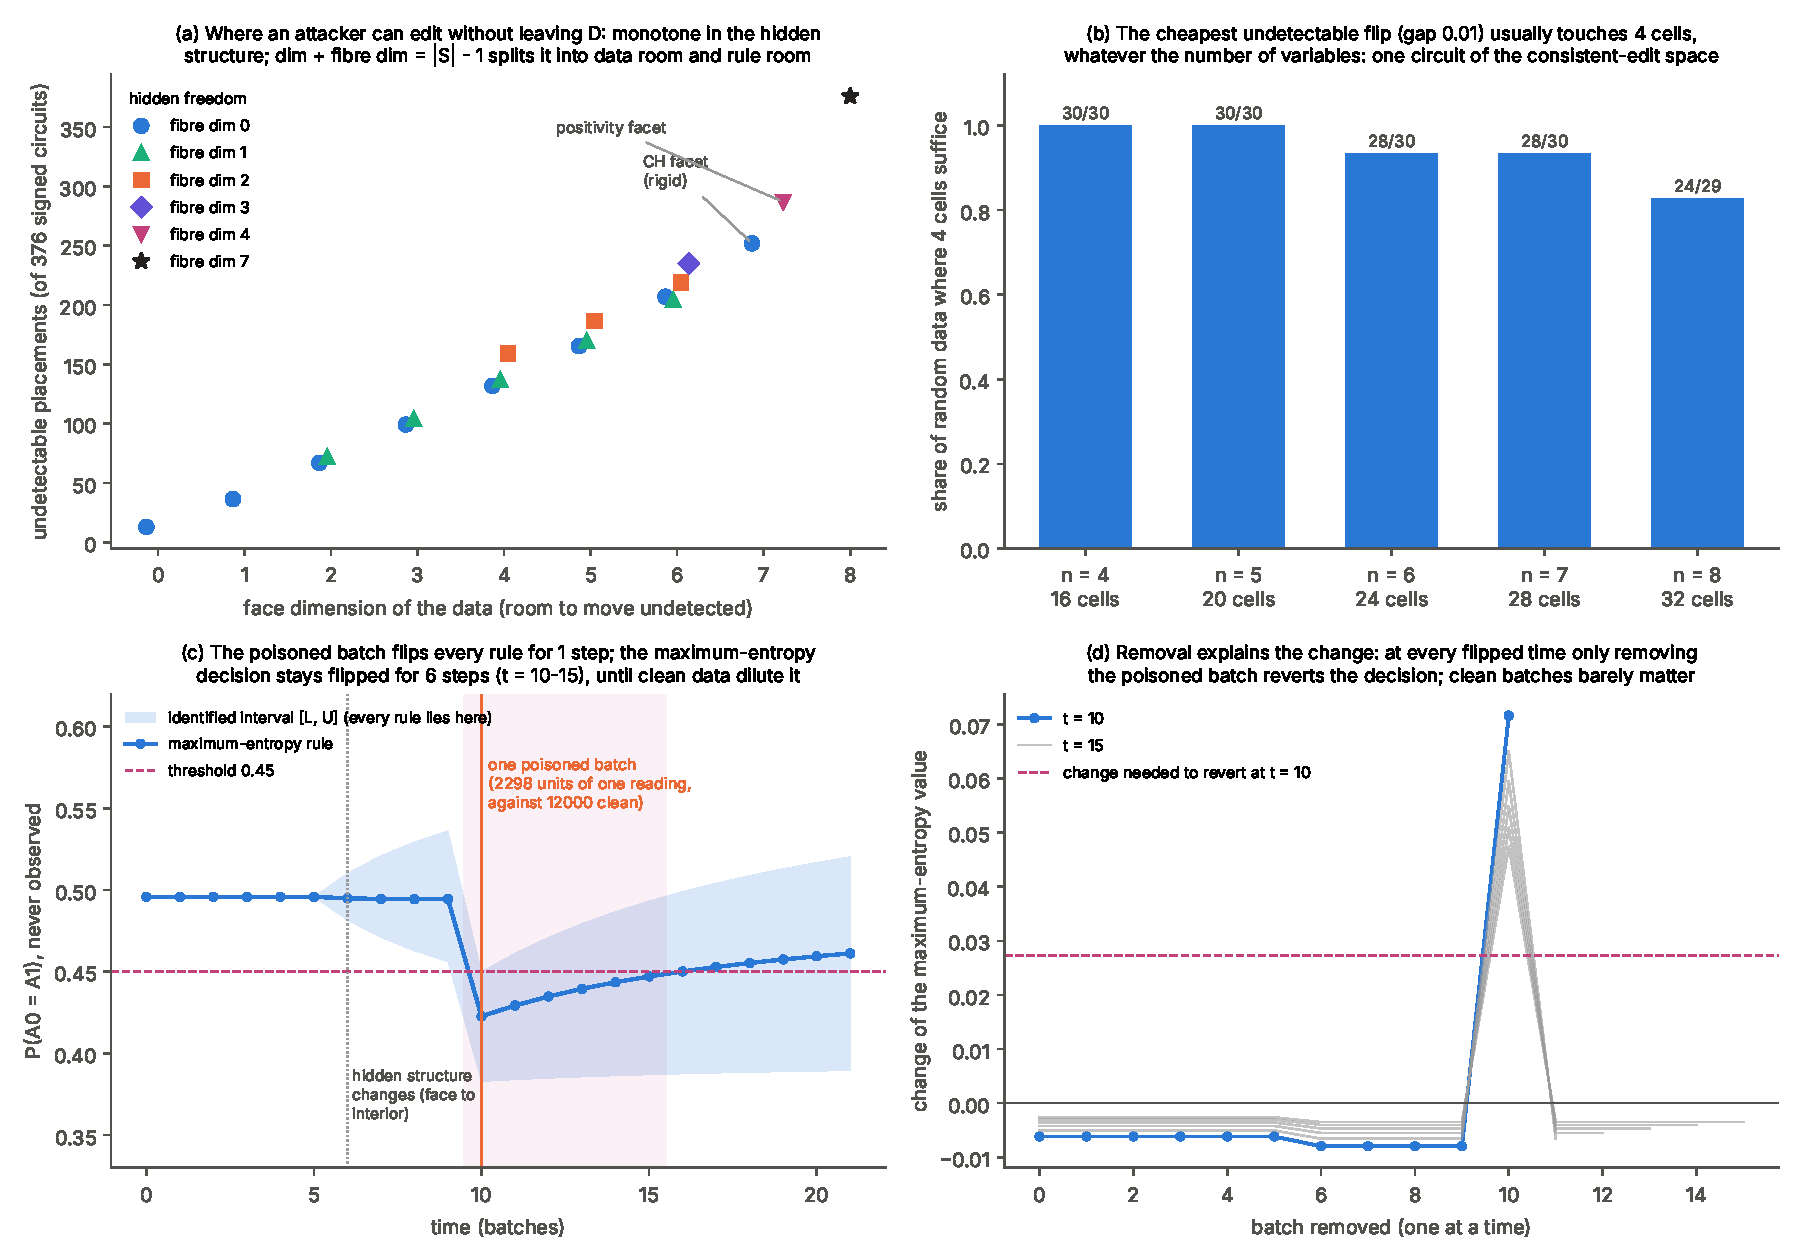
\includegraphics[width=\linewidth]{fig_poisonflip.pdf}
\caption{How little poisoning. (a) Undetectable placements (signed circuits that keep the data in $\mathcal D$) against the face dimension of the data, by fibre dimension, over all $2721$ faces of the 4-cycle. The count is monotone in the hidden structure, and $\dim G+\dim(\text{fibre})=|S|-1$ splits that structure into room for the data and room for the rule. (b) The cheapest undetectable flip (gap $0.01$) is usually one circuit of $4$ cells, for every $n$ up to $8$. (c) One poisoned batch at $t=10$, after the hidden structure changed at $t=6$. The identified interval (shaded) flips below the threshold for one step; the maximum-entropy rule stays flipped for six. (d) Removing one batch at a time at the flipped times: only the poisoned batch reverts the decision.}\label{fig:poisonflip}
\end{figure}

What is proved here is elementary: the two thresholds, the circuit bound, monotonicity of placement, the removal laws and the additivity of cost over conformal sums. The circuit census and the face table are exact computations, and the frequencies of one-circuit optima, the budget comparison and the time example are numerical. We have not found these statements for marginal data in the literature on poisoning, which counts records or input coordinates.

\subsection{The geometry of poisoning}\label{sec:poisongeom}
A poisoning edit moves the data $d$, and with them the fibre $J_d$ of compatible joint laws. Three effects can be separated: the fibre can \emph{deform} (change dimension or size), the data can \emph{cross} the contextuality boundary (the fibre empties), and the \emph{selected} law can move. \Cref{sec:poisondim} gave the costs of flips. Here each effect gets a precise statement, and the decision gets a radius that the defender can compute from the data alone.

\begin{proposition}[certified radii and the three effects]\label{prop:radii}
Let $\mathcal V_L$ and $\mathcal V_U$ be the dual vertices with $L(d)=\max_{(y,y_0)\in\mathcal V_L}(y\cdot d+y_0)$ and $U(d)=\min_{(y,y_0)\in\mathcal V_U}(y\cdot d+y_0)$, and let $\mathcal C_1$ be the circuits scaled to unit cost.
\begin{enumerate}
\item[(1)] \emph{Certified radii.} $L$ and $U$ are Lipschitz in the edit cost, with constants $\Lambda_L=\max_{\mathcal V_L\times\mathcal C_1}|y\cdot C|$ and $\Lambda_U=\max_{\mathcal V_U\times\mathcal C_1}|y\cdot C|$. Hence $c_{\rm some}(d)\ge(L(d)-\tau)/\Lambda_L$ and $c_{\rm all}(d)\ge(U(d)-\tau)/\Lambda_U$.
\item[(2)] \emph{Deformation.} The width $U-L$ changes by at most $(\Lambda_L+\Lambda_U)\,c(\delta)$, while the fibre dimension can jump. By \cref{thm:projection} it rises from $|V(G)|-1-\dim G$ to $|V(G')|-1-\dim G'$ when an edit moves the data from a face $G$ into a larger face $G'$.
\item[(3)] \emph{Crossing.} The cost distance from $d\in\mathcal D$ to the contextuality boundary is $\min_h \sigma_h(d)/\max_{C\in\mathcal C_1}(-h\cdot C)$ over the CH facets $h\cdot d+h_0\ge0$, where $\sigma_h(d)=h\cdot d+h_0$ is the slack. Along a line $d+tv$, the data first become contextual at $t=\min\{\sigma_h(d)/(-h\cdot v):h\cdot v<0\}$, and from then on the fibre is empty and the contextual fraction positive.
\item[(4)] \emph{Selection.} $L$ and $U$ are continuous whatever the rule. A section given by a continuous objective with a unique optimum on every fibre (maximum entropy, or a fixed linear objective with unique optima) is continuous on $\mathcal D$. A selected law can jump only through ties or a rule that depends on the data discontinuously.
\end{enumerate}
\end{proposition}

\begin{proof}
(1) A maximum (or minimum) of affine functions is Lipschitz with constant equal to the largest dual norm of their gradients. The dual norm of $y$ for the cost $c$ is $\max y\cdot\delta$ over the unit cost ball, whose extreme points are the unit circuits \cite{Rockafellar1969}. A flip must move $L$ (resp.\ $U$) by $L-\tau$ (resp.\ $U-\tau$). (2) Apply (1) to both ends. The dimension statement is \cref{thm:projection}. (3) In a polyhedral norm, the distance to a hyperplane is the slack divided by the dual norm of its normal. For a point of a convex polytope, the distance to the boundary is the least distance to a facet hyperplane. The line formula is the first zero of the slacks. (4) The fibre map is continuous with compact values, being Lipschitz \cite{WalkupWets1969}. By Berge's maximum theorem the optimal set is upper hemicontinuous, hence continuous where it is a single point. $L$ and $U$ are optimal values, which (1) shows to be Lipschitz.
\end{proof}

For the decision quantity $P(A_0=A_1)$ on CHSH, the constants are exact (PG1). There are six dual vertices on each side and $376$ unit circuits, and $\Lambda_L=\Lambda_U=1$; for $P(A_0=0,A_1=0)$ both constants are $1/2$. So no undetectable flip of the some-rule decision costs less than the gap $L-\tau$. Over $75$ cases at $39$ data points the bound is attained in $45$ and is never off by more than a factor $2$ (PG2). For every rule the median ratio of the actual cost to the bound is $1.10$. The distance formula in (3) agrees with a direct linear program to machine precision (PG4). Along $20$ straight data paths, both maximum entropy and a fixed-objective vertex rule move by at most $0.019$ in total variation per step of $0.01$ (PG6). So, unlike what one might expect, rules that pick vertices do not jump as the data move, as long as their optimum is unique. What poisoning can make discontinuous is the decision at its threshold, and the dimension of the fibre, but not its width and not a well-defined rule.

\begin{example}[poisoning in stages]\label{ex:stages}
Start from the first CH-facet law of Study 18, where $P(A_0=A_1)=0.496$ is identified (the fibre is a point), with $12000$ clean units and threshold $\tau=0.45$ (PG5, \cref{fig:deform}). Compare two poisoning routes that add units of a single reading.
\begin{itemize}
\item \emph{Route A}, the cheapest every-rule attack, injects the reading $(0,1,1,0)$. That reading is a vertex of the same CH facet, so the data slide along the facet. At $600$, $1200$ and $1800$ units the fibre is still a point, with $L=U=0.472$, $0.451$, $0.431$. Some rule and every rule flip together, at a poisoned share of $0.0924$ (about $1222$ units).
\item \emph{Route B} injects $(1,0,1,0)$, which lies off the facet. After the first unit the fibre dimension jumps from $0$ to $7$, but the width starts at $0$ and grows at most twice as fast as the cost. The interval is $[0.472,0.567]$ at $600$ units, $[0.451,0.633]$ at $1200$, $[0.413,0.747]$ at $2400$, $[0.354,0.640]$ at $4800$ and $[0.275,0.498]$ at $9600$. Some rule flips at the same share $0.0924$, but every rule flips only at $0.4977$, about $11900$ units: $5.4$ times the share and nearly ten times the units. The maximum-entropy value first rises to $0.516$ and falls below $\tau$ only after about $6060$ units. The distance to the contextuality boundary is $0$ throughout route A, and on route B it is $0.095$, $0.182$, $0.333$, $0.571$ and $0.500$ at those stages.
\item \emph{Overreach.} Mix in the PR box that violates this CH facet. From the rigid start the data become contextual at once: the fibre is empty and the contextual fraction positive for every share above $0$. From route B at $2400$ units they become contextual at share $0.2501$, where the facet slacks predict $0.2500$. In all $31$ cases the fibre is empty exactly when the contextual fraction is positive.
\end{itemize}
\end{example}

The cheapest attack on a rigid point keeps the point rigid. It slides along the facet, so the decision stays identified and simply moves. Deformation is what an attack off the facet produces, and it buys ambiguity rather than a decision: the interval straddles the threshold for a long time before every rule flips. A defender who reports $[L,U]$ sees route B as rule-dependent from share $0.0924$ on, and route A as a clean flip. At a rigid point, complete determination lies next to inconsistency. One contextual push empties the fibre and is detected at once. So an attacker must stay inside $\mathcal D$, and a contextuality alarm is free for the defender. The literature's geometries of poisoning (bilevel, influence, metric) describe the learner. These statements describe the space of compatible explanations. The two meet in the first-order estimate of \cref{rem:cellattr}.

\begin{figure}[!htbp]\centering
\includegraphics[width=\linewidth]{fig_deform.pdf}
\caption{The geometry of poisoning, in stages (\cref{ex:stages}). (a) The shadow of the fibre on two never-observed quantities. From a rigid CH-facet point (star), route A (diamonds) stays a point; route B opens into polygons as poisoned units are added (labels), with the maximum-entropy law inside. (b) The identified interval: the same share flips some rule on both routes, but flipping every rule off the facet takes nearly ten times as many units. (c) Distance to the contextuality boundary. (d) A PR-box overreach: from the rigid point any contextual push empties the fibre; from inside, exactly where the facet slacks predict. (e) Certified radii against actual cheapest flips. (f) Width change against edit cost: the dimension jumps, the width obeys the Lipschitz bound.}\label{fig:deform}
\end{figure}

\subsection{Bayesian inversion and sections}\label{sec:invsec}
Bayesian inversion reverses a stochastic map relative to a prior. From $p$ and $K(y\mid x)$ it gives $q=pK$ and $K^\dagger(x\mid y)=p(x)K(y\mid x)/q(y)$ wherever $q(y)>0$. Categorically it is disintegration of the joint law in the other direction \cite{ChoJacobs2019}. Parzygnat separates ordinary inverses, disintegrations and Bayesian inverses, and extends them to quantum Markov categories \cite{Parzygnat2020}. Bohinen and Perrone show that when an (a.s.-compatibly representable) Markov category has conditionals, the multiplication of its probability monad is weakly cartesian \cite[Thm.~3.1]{BohinenPerrone2025}. This covers the Giry monad on standard Borel spaces \cite[Cors.~3.2, 3.9]{BohinenPerrone2025}. They avoid calling the property a Beck--Chevalley condition, because that term has a different established meaning for fibrations and descent \cite[Rem.~2.25]{BohinenPerrone2025}. \Cref{rem:beckchevalley} uses the term only for our own reading. This subsection places inversion relative to sections.

\begin{proposition}[inversion and sections]\label{prop:invsec}
\begin{enumerate}
\item[(1)] In $\mathsf{Cpl}$ the dagger is Bayesian inversion: if $\gamma(x,y)=p(x)K(y\mid x)$, then $\gamma^{\!\top}(y,x)=q(y)K^\dagger(x\mid y)$. The dagger is total, although inversion of kernels is partial: at a null event every choice of $K^\dagger(\cdot\mid y)$ gives the same $\gamma^{\!\top}$. So for one coupling, inversion is a symmetry and not a choice. Given the prior and the kernel, the fibre is a point.
\item[(2)] Let $s$ be a section of the chain cover that is reversal-equivariant: $x_{ijk}\mapsto x_{kji}$ carries $s(\gamma_1,\gamma_2)$ to $s(\gamma_2^{\!\top},\gamma_1^{\!\top})$. Then composition by $s$ commutes with inversion: $(\gamma_1\circ_s\gamma_2)^{\!\top}=\gamma_2^{\!\top}\circ_s\gamma_1^{\!\top}$. Markov gluing (the dagger functor of $\mathsf{Cpl}$) and selection (\cref{prop:selkeeps}(3)) both qualify.
\item[(3)] A rule that is not reversal-equivariant need not commute. The vertex of the chain fibre minimising $\sum G_iH_kx_{ijk}$, with $G=(0,2,1,3)$ and $H=(0,1,2,3)$, commutes on only $13$ of $40$ random chains with ends of up to $3$ states. On chains with binary ends, every rule that minimises a fixed linear objective with a unique optimum commutes.
\item[(4)] Null events never reach a composite, while structural zeros do matter. A middle state with $q(y)=0$ contributes nothing to any composite, whatever kernel is attached to it. A zero cell with full-support margins leaves every Bayesian inverse unique, yet the composite's identified interval keeps positive width, so the rule still decides.
\end{enumerate}
\end{proposition}

\begin{proof}
(1) $\gamma^{\!\top}(y,x)=p(x)K(y\mid x)=q(y)K^\dagger(x\mid y)$, and the row of a null $y$ is $0$ whatever $K^\dagger(\cdot\mid y)$ is. (2) Reversal maps the fibre of $(\gamma_1,\gamma_2)$ bijectively onto that of $(\gamma_2^{\!\top},\gamma_1^{\!\top})$. The end marginal of a reversed table is the transpose of the end marginal. (3) For binary ends the fibre is the box $\prod_b[L_b,U_b]$ in the coordinates $x_{0b0}$, which reversal fixes. A linear objective acts on it through the coefficients $c_{0b0}-c_{0b1}-c_{1b0}+c_{1b1}$, which reversal also fixes, so the optimum is the same point. The count is exact (IS3). (4) The row $y$ of $\gamma_2$ is $q(y)K(y,\cdot)=0$ (IS4). The interval is exact on six chains with a zero cell (IS5), where Markov gluing and selection disagree in five. In the sixth, Markov gluing happens to be the midpoint. IS1 and IS2 check (1) and (2) exactly on $60$ and $40$ random rational examples.
\end{proof}

So the question whether Bayesian inversion is a canonical section of the marginal projection has a precise answer. It is not a section but a symmetry of the projection. Every composition rule that respects the symmetry commutes with it, and a rule that does not respect it can fail to commute; we have not shown that every rule that commutes is reversal-equivariant. A prior and a kernel determine the joint law, so inverting them involves no selection. Selection enters only when the joint law is not determined, as for the composite of a chain, and there it is compatible with inversion when the rule is reversal-equivariant. Information destroyed by a map is not recovered by inverting it. In the merging example $f(a)=f(b)=0$, $f(c)=1$ with prior $(0.2,0.5,0.3)$, the inverse $P(a\mid0)=2/7$, $P(b\mid0)=5/7$ is fixed by the prior, not chosen.

\begin{remark}[order drift as Bayesian inconsistency]\label{rem:orderbayes}
A model that generates variables one at a time defines, for each order $\sigma$, a joint law $Q_\sigma$, the product of its conditionals in that order. Bayes' rule between two orders says $Q_\sigma=Q_{\sigma'}$: the conditionals of one order are the Bayesian inverses of the other's. The order drift of Studies 17 and 18, the mean total variation between the $Q_\sigma$, therefore measures how far a learned model is from being a single probabilistic object that inverts consistently. Study 18's consistency penalty is the squared residual of Bayes' rule in log form at sampled assignments. On the sparsity-matched faces it lowered the drift from $0.315$, $0.281$ and $0.174$ to $0.011$, $0.007$ and $0.010$ (IS6, from the frozen output). A model with drift has no single joint law and so no single inverse: a question asked forward and backward can get answers that no joint law reconciles. By \cref{prop:invsec}(2), only a coherent model whose completion rule is reversal-equivariant answers both directions consistently.
\end{remark}

\subsection{The geometry of decisions and of the value of information}\label{sec:voi}
The fibre $J_d$ is a credal set in the sense of imprecise probability: a polytope of compatible laws, finitely generated by its vertices. This subsection asks which part of its geometry matters for a decision, what information is worth, and how stable a decision is under a disturbance whose cause the decision-maker cannot see. Actions $a$ carry utilities $u_a$ on joint readings, so $\mathbb E_Pu_a=u_a\cdot P$ is linear in $P$. Two kinds of information are kept apart:
\begin{itemize}
\item \emph{structural} information is a new context, a pair never measured together; it shrinks the fibre;
\item \emph{instance} information is a signal $Z$ about one unit's state; it leaves the population fibre unchanged.
\end{itemize}

\begin{proposition}[decisions over a fibre]\label{prop:decisions}
\begin{enumerate}
\item[(1)] The utility image $\{(u_a\cdot P)_a:P\in J_d\}$ is a polytope. A decision is \emph{identified}, meaning one action is optimal for every compatible law, exactly when the image lies in one cell of the arrangement of indifference hyperplanes $u_a\cdot P=u_b\cdot P$. The fibre's dimension plays no role.
\item[(2)] The value of resolving the fibre, under minimax regret, is $R(d)=\min_a\max_b U_{ab}(d)$, where $U_{ab}$ is the upper end of the identified interval of $(u_b-u_a)\cdot P$. It needs $|A|^2$ linear programs, and $R(d)=0$ exactly when the decision is identified. If $a_0$ is optimal for some law in $J_d$, then $R\le\max_b(U_{a_0b}-L_{a_0b})$, so resolving the fibre is worth at most its width along utility differences. $R$ is Lipschitz in the edit cost, with constant the largest Lipschitz constant of the $U_{ab}$ (\cref{prop:radii}(1)). Observing more contexts never raises it. It is $0$ on a rigid face for every utility.
\item[(3)] Mixing data mixes fibres: $\lambda J_d+(1-\lambda)J_{d'}\subseteq J_{\lambda d+(1-\lambda)d'}$. So along any segment of data $L$ is convex and $U$ and the width $U-L$ are concave. Poisoning by adding batches moves along such segments.
\item[(4)] Take \emph{act} and \emph{abstain} with symmetric payoffs $\mathbb 1[A_0=A_1]-\tau$ and $\tau-\mathbb 1[A_0=A_1]$. Then $R=2\min\{(\tau-L)_+,(U-\tau)_+\}$, which is concave along segments where it is positive. The value of randomising, the gain of the best mixed action over the best pure action under the worst compatible law, is exactly $R/2$.
\end{enumerate}
\end{proposition}

\begin{proof}
(1) A linear image of a polytope is a polytope, and an action is optimal throughout $J_d$ exactly when every $U_{ab}\le0$. (2) Minimax regret over a convex set of laws and finitely many actions: the inner maximum over $P$ of $(u_b-u_a)\cdot P$ is a linear program. If $a_0$ is optimal at $P_0\in J_d$, every $L_{a_0b}\le0$, so $U_{a_0b}\le U_{a_0b}-L_{a_0b}$. Lipschitz continuity: minima and maxima preserve Lipschitz constants. Monotonicity: more contexts give a smaller fibre, hence smaller maxima. Rigid faces: every $U_{ab}=-U_{ba}$, so some action has all $U_{ab}\le0$. (3) Convex combinations of compatible laws are compatible with the combined data, and $L$ and $U$ are optimal values over these sets. (4) Here $U_{\rm act,abstain}=2(\tau-L)$ and $U_{\rm abstain,act}=2(U-\tau)$. Each is concave along a segment, and so is their minimum. Acting with probability $x$ earns $(2x-1)(\phi-\tau)$. When $L<\tau<U$, the choice $x=1/2$ guarantees $0$, while the best pure action guarantees $-\min(\tau-L,U-\tau)$. Checks VG1--VG3 and VG5 test this numerically: the Lipschitz ratio is at most $0.53$ over $40$ pairs, and removing a context raises $R$ in $118$ of $120$ cases.
\end{proof}

\begin{proposition}[instance information]\label{prop:instance}
Let $Z$ be a signal of accuracy $\alpha$ about $T=\mathbb 1[A_0=A_1]$, and let $\phi=P(T=1)$. For the payoffs of \cref{prop:decisions}(4), write $a_z=P(T=1,Z=z)-\tau P(Z=z)$.
\begin{enumerate}
\item[(1)] Under a single law (any section), the value of the signal is $\sum_z|a_z|-|\sum_za_z|\ge0$. This is Good's inequality as a triangle inequality \cite{Das2023}. It is $0$ exactly when no posterior lies on the other side of $\tau$ from the prior, so the signal has decision value only when it can move the decision.
\item[(2)] A robust decision-maker who commits to a policy $z\mapsto a$ can always ignore the signal, so the signal's robust value is never negative \cite{Iskandar2026}.
\begin{itemize}
\item With mixed policies allowed, the minimax theorem makes the robust value $\min_{\phi\in[L,U]}\sum_z|a_z|-\min_{\phi\in[L,U]}|\phi-\tau|$, which is $0$ for an uninformative signal.
\item With pure policies only, the robust value equals the mixed-policy value plus the value of randomising without the signal, minus the value of randomising with it.
\end{itemize}
\item[(3)] Information and value differ. Below a critical accuracy the signal has positive mutual information with $T$ but no decision value. For fixed $\phi$ the value is largest when $\tau=\phi$, whereas the entropy of $T$ does not depend on $\tau$.
\end{enumerate}
\end{proposition}

\begin{proof}
(1) The Bayes value with the signal is $\sum_z|a_z|$ and without it $|\sum_za_z|$; the triangle inequality is an equality exactly when all $a_z$ share a sign. (2) Constant policies are available, so the maximum over policies cannot fall. Payoffs are linear in $\phi$ and in the mixture, so the minimax theorem applies, and the robust value with mixing is the minimum over $\phi$ of the Bayes value. The decomposition for pure policies holds by definition. (3) Below the critical accuracy both posteriors stay on the prior's side of $\tau$. Checks VG4 and VG7 test this.
\end{proof}

\begin{theorem}[when local data determine the value of information]\label{thm:determination}
Let $Z=z(\omega)$ be a signal that is a function of the reading. Its classical value $\mathrm{VOI}(P)=\sum_z\max_a(u_a\mathbb 1_{z})\cdot P-\max_au_a\cdot P$ is continuous and piecewise linear on $J_d$. On each \emph{policy cell}, where the action $a_0$ without the signal and the rule $z\mapsto a_z$ with it are both optimal, it equals $g\cdot P$ for the \emph{value functional} $g=\sum_z\mathbb 1_z\,(u_{a_z}-u_{a_0})$. The following are equivalent:
\begin{enumerate}
\item[(i)] the local data determine the value of information: $\mathrm{VOI}$ is constant on $J_d$;
\item[(ii)] the value functional of every policy cell that is full-dimensional in $J_d$ is orthogonal to the direction space of $J_d$;
\item[(iii)] on the support of the fibre, each such value functional is \emph{cover-additive}, a sum $\sum_kh_k(\omega_{C_k})$ of functions of the observed contexts.
\end{enumerate}
In particular, a determined global law determines the value of information. A determined value does not determine the law, and determination of the value is independent of whether the decision itself is identified ($R=0$).
\end{theorem}

\begin{proof}
On a policy cell each maximum is attained by the cell's actions, so $\mathrm{VOI}=g\cdot P$ there. The cells are polyhedra, finitely many, and they cover $J_d$. (i)$\Rightarrow$(ii): on a full-dimensional cell, a direction $v$ of $J_d$ with $g\cdot v\ne0$ changes $\mathrm{VOI}$ inside the cell. (ii)$\Rightarrow$(i): the full-dimensional cells cover $J_d$, because the others lie in finitely many proper affine subspaces. $\mathrm{VOI}$ is continuous and has zero derivative along $J_d$ on each full-dimensional cell, so it is constant on the connected set $J_d$. (ii)$\Leftrightarrow$(iii): on the fibre's support $S$, the direction space is $\{v:\ v|_{S^c}=0,\ \pi v=0,\ \mathbf 1\cdot v=0\}$. Its orthogonal complement, restricted to $S$, is the span of the rows of the marginal map, that is, of the indicators of context events. For the last sentence: a point fibre has no directions. The cases below show the other two claims.
\end{proof}

The criterion is checkable: the cells are cut out by linear inequalities, and full-dimensionality is a slack linear program. The envelope $[\min,\max]$ of $\mathrm{VOI}$ over $J_d$ is computed exactly by one linear program per cell and sense. On $80$ random problems (cover-additive or general utilities; signals on one variable or a parity of two; interior data and the fibre-$0$, $1$ and $2$ faces of Study 18), the criterion holds exactly when the envelope is a point, in all $80$ (VD1). The four cases of \cref{fig:voidet}(a), each with the signal $B_0$ (VD2):
\begin{itemize}
\item On a rigid face the value of information is determined ($0.081$), because the law is.
\item In the interior, with a decision and a signal inside the context $(A_0,B_0)$, the fibre has dimension $7$ and the value is still determined ($0.081$).
\item The running decision on the never-observed pair is not determined: the value ranges over $[0,0.292]$.
\item An identified decision ($R=0$) can still have an undetermined value: $[0,0.201]$.
\end{itemize}
The three determinations (of the global law, the decision and the value of information) therefore separate. When the value functional lives in one context, the value of information is computed from that table alone, so it stays defined for contextual data, where no global law exists. For a decision on $A_0=0$ with the signal $B_0$, a PR box (contextual fraction $1$) has value $0.45$ (VD3). This is the decision-value counterpart of the reconstruction of global choices from local problems in \cite{TohmeCaterinaGangle2017}: there, local optima glue exactly when the local utilities come from one global function. Here, the value of information glues exactly when the value functionals are sums over the contexts.

\begin{figure}[!htbp]\centering
\includegraphics[width=\linewidth]{fig_voidet.pdf}
\caption{Determination of the value of information (\cref{thm:determination}) and value-based distance (\cref{prop:valuedist}). (a) The exact envelope of the classical value of the signal $B_0$ over the fibre in four cases: the global law, the decision ($R$) and the value of information are determined independently. (b) On $80$ random problems, the criterion's residual and the envelope's width vanish together. (c) The largest change in robust value over utilities in $[-1,1]$ equals twice the Hausdorff distance between the fibres, and is attained by the dual utility.}\label{fig:voidet}
\end{figure}

\begin{example}[what information is worth on the staged routes]\label{ex:voi}
Read \cref{ex:stages} through these quantities, with $\tau=0.45$ (VG6--VG8, \cref{fig:voi}).
\begin{itemize}
\item \emph{Route A} keeps the fibre a point, so $R=0$ at every stage, although the decision flips at about $1222$ poisoned units. A robust decision-maker sees no reason to collect more data: the cheapest attack is invisible to value-of-information monitoring. The signal about the unit is still worth up to $0.296$, most near $1200$ units, where the selected value $0.451$ sits on the threshold.
\item On \emph{route B}, $R$ is positive exactly between $1222$ and $11890$ units, where the interval straddles the threshold, and is concave there. It peaks at $0.258$ near $6550$ units, and randomising recovers half of it. The fibre's shadow at $2400$ units is cut by the threshold into the laws that favour each action, and $R$ is twice the smaller overhang, $2\times0.037$.
\item \emph{Envelope.} With pure policies, the robust value of a signal of accuracy $0.8$ leaves the envelope of classical values over the fibre: at $2400$ units it is $0.332$ against $[0.018,0.297]$, and at $6000$ units $0.409$ against $[0.159,0.297]$. It does so by exactly the value of randomising, $0.037$ and $0.119$. With mixed policies the robust value is $0.295$ and $0.290$, inside the envelope.
\item \emph{Three gains.} At $2400$ units the three gains from one signal differ. The identification gain is $0$, since the fibre is unchanged. The information gain $I(T;Z)$ rises smoothly from accuracy $1/2$. The Bayes decision gain is $0$ until the critical accuracy $0.566$ and linear after it. The robust gain with mixing has no kink there, because under ambiguity the robust baseline is already the randomised $0$.
\end{itemize}
\end{example}

\begin{figure}[!htbp]\centering
\includegraphics[width=\linewidth]{fig_voi.pdf}
\caption{What information is worth (\cref{ex:voi}). (a) The fibre's shadow at $2400$ units on route B, cut by the threshold into laws favouring each action: the value of identification is twice the smaller overhang. (b) The value of identification along both routes: route A flips the decision with no value of information at all. (c) A signal about the unit along route B: Bayes under maximum entropy, the robust value with pure and with mixed policies, and the envelope of classical values over the fibre. (d) Information, identification and decision gains against the signal's accuracy. (e) The value of the signal and of identification against the threshold: largest at the decision boundary. (f) Dilation: observing $B_0$ can widen the interval of the never-observed quantity, though never on a rigid face.}\label{fig:voi}
\end{figure}

\begin{proposition}[value-based distance is Hausdorff distance]\label{prop:valuedist}
For $d,d'\in\mathcal D$,
\[\sup\Big\{\big|\max_a\min_{P\in J_d}u_a\cdot P-\max_a\min_{P\in J_{d'}}u_a\cdot P\big|:\ |u_a|\le1\Big\}=2\,d_H^{\rm TV}(J_d,J_{d'}),\]
and the supremum is attained by a single action. So the worst-case change in robust decision value, over all bounded decision problems, is the Hausdorff distance between the sets of compatible laws.
\end{proposition}

\begin{proof}
For one action the robust value is the support function $h_J(u)=\min_{P\in J}u\cdot P$. For convex compact sets, $\sup_{\|u\|_*\le1}|h_J-h_{J'}|$ is the Hausdorff distance in the norm whose dual is $\|\cdot\|_*$. Here $\|\cdot\|_*=\|\cdot\|_\infty$, so the distance is in $\ell_1$, which is twice total variation. A maximum over actions of $1$-Lipschitz functions of the set is again $1$-Lipschitz, so several actions cannot exceed the bound. VD4 finds the attaining utility from the linear-programming dual of the $\ell_1$ distance from the farthest vertex. It reaches $2d_H^{\rm TV}$ to $10^{-7}$ on six random pairs, while $300$ random utilities and $60$ random three-action problems stay below.
\end{proof}

This is the counterpart, for credal fibres, of the value-based distance between information structures of Gensbittel, \Peski{} and Renault \cite{GensbittelPeskiRenault2022}. It answers how the two kinds of stability are connected: the credal-stability numbers above are, exactly, worst-case changes in robust decision value.

\paragraph{Stability, from the decision-maker's side.} A model that keeps accepting data cannot tell genuine drift from fluctuation or poisoning. Histories that are equally likely under drift and under poisoning cannot be told apart by any procedure that sees only the history. So what matters to the decision-maker is how far a recommendation can be disturbed, whatever the cause. Five quantities answer this, and they are different.
\begin{itemize}
\item \emph{Decision invariance.} The least edit cost that changes the recommendation is the certified radius of \cref{prop:radii}: no undetectable disturbance smaller than $(L-\tau)/\Lambda_L$ can flip a decision that some rule would make, nor one smaller than $(U-\tau)/\Lambda_U$ for every rule.
\item \emph{Worst-case regret.} This is $R$, which is Lipschitz and so moves at most $2$ per unit of cost in the example.
\item \emph{Credal stability.} The Hausdorff distance in total variation between fibres, computed exactly from their vertices (half the worst-case change in robust decision value, by \cref{prop:valuedist}), stays within $1.11$ times the edit cost along route B. It is $0.007$, $0.029$, $0.157$ and $0.456$ after $25$, $100$, $600$ and $2400$ units, while the fibre dimension jumps from $0$ to $7$ at the first unit.
\item \emph{Dilation.} Observing $B_0$ widened the interval of $P(A_0=A_1)$ for some outcome at all $300$ random data points tested, and for every outcome at $9$. One example goes from $[0.499,0.806]$ to $[0.334,0.987]$ and $[0.130,0.850]$. This is the dilation of imprecise probability, which Das identifies as the source of failures of the value of evidence \cite{Das2023}. It never occurs on a rigid face.
\item \emph{Diachronic stability} in Das's sense: commit to one law in the credal set and act by its conditionalisations \cite{Das2023}. A section is such a commitment, and the square ``select, then condition'' against ``condition, then select'' tests it. On marginal data the square fails structurally: after conditioning on $B_0=z$ only the contexts containing $B_0$ stay observable, so re-selecting uses less information. The re-selected maximum-entropy law differs from the committed one by $0.084$ to $0.274$ in total variation at random points. On the rigid faces it differs by $0.220$ to $0.459$, and the decision value there by up to $0.189$, because re-selection throws away a fully identified law (VG8). Commitment is therefore the stable policy here, and Good's inequality holds for it by \cref{prop:instance}(1).
\end{itemize}
The order drift of learned models (\cref{rem:orderbayes}) is a failure of exactly this commitment. Stability is not safety: a stable model can be poisoned along route A, and an unstable one may be tracking genuine change. Dynamically, pooling makes a single disturbance decay like $1/N_t$, with no exponential rate, and \cref{prop:removal}(3) gives the exact duration of a one-batch flip. Under exponential forgetting at rate $\eta$, disturbances decay at the Lyapunov rate $\log(1-\eta)<0$. Whether topological summaries of a decision trajectory (persistent homology of sliding windows, braids formed by the ranked values of competing actions) warn before the decision margin closes is a question for a controlled study, not settled here.
\paragraph{Relation to the literature.} The ingredients of this subsection are established. What is new is their joint quantitative treatment over marginal fibres.
\begin{itemize}
\item Abramsky and Brandenburger characterise when local tables glue to a global law \cite{AbramskyBrandenburger2011}, with cohomological witnesses of failure \cite{AbramskyMansfieldBarbosa2012}. The contextual fraction measures an operational advantage in games and computation \cite{AbramskyBarbosaMansfield2017}, which is not the decision value of acquiring information.
\item Vigneaux's information cohomology characterises entropy as a cocycle \cite{Vigneaux2020}; an entropy is not a value of information.
\item Tohm\'e, Caterina and Gangle treat the reconstruction of global choices from local problems sheaf-theoretically, and identify contextuality as an obstruction to it \cite{TohmeCaterinaGangle2017}. \Cref{thm:determination} is the analogous statement for the value of information.
\item Iskandar separates a rule-specific value of information from the envelope of classical values over a credal set, and gives non-negativity under $\Gamma$-maximin with constant policies \cite{Iskandar2026}. \Cref{prop:instance}(2) agrees, and adds the exact decomposition of the excess over the envelope into the value of randomising.
\item Das's practical stability \cite{Das2023} is the commitment that a section provides.
\item Gensbittel, \Peski{} and Renault measure information structures by value \cite{GensbittelPeskiRenault2022}; \cref{prop:valuedist} does so for credal fibres.
\end{itemize}
Our contribution is the combination over marginal fibres: identified decisions, the regret from ambiguity that cannot be resolved, structural against instance information, when local data determine the value of information, and how all of these respond to poisoning.


\paragraph{Fisher geometry and decision relevance.} Moskowitz, Russell and Lawless propose to value information information-geometrically \cite{MoskowitzRussellLawless2020}. Laws form a statistical manifold with the Fisher metric $g$, and they call information valuable at a point when it increases the ``complexity'' $\sqrt{\det g}$, the coefficient of the volume form. In the normal family a change of mean then has null value, and a decrease of the standard deviation is valuable. The toric K\"ahler structure of \cref{prop:kahler} carries the same metric, with the phases of the torus as further coordinates. The next proposition places all of this against the decision geometry of this subsection.

\begin{proposition}[Fisher geometry and decision relevance]\label{prop:fisher}
\begin{enumerate}
\item[(1)] \emph{Phases are decision-null.} Every expected utility, hence every robust value, regret and value of information, depends on an amplitude $z=\sqrt P\,e^{i\theta}$ only through $P=|z|^2$. On real amplitudes the Fubini--Study distance is half the Fisher--Rao distance $d_{\rm FR}(P,Q)=2\arccos\sum_x\sqrt{P_xQ_x}$.
\item[(2)] \emph{The fibre is the Fisher-null space of the data.} At an interior law, the Fisher information of one reading in each observed context, $I_{\rm obs}=\sum_cA_c^{\!\top}\operatorname{diag}(1/A_cP)A_c$ on $\{v:\mathbf 1\cdot v=0\}$, has null space exactly the direction space of $J_d$. The Fisher information of a complete reading is positive definite. So the criterion of \cref{thm:determination} says: the value of information is determined exactly when every full-dimensional cell's value functional is \emph{Fisher-visible}, i.e.\ annihilates the null space of $I_{\rm obs}$.
\item[(3)] \emph{Decision value is Lipschitz in Fisher--Rao distance.} For utilities with $|u|\le1$, $|u\cdot P-u\cdot Q|\le2\,\mathrm{TV}(P,Q)\le2\sqrt{1-\mathrm{BC}^2}=2\sin(d_{\rm FR}/2)$, where $\mathrm{BC}=\sum\sqrt{P_xQ_x}$.
\item[(4)] \emph{The converse fails both ways.} Points of one fibre can be far apart in Fisher--Rao distance and have the same value of information. Points at Fisher--Rao distance tending to $0$ can lie on either side of a policy wall and take different actions; only the value is continuous.
\item[(5)] \emph{Volume coefficients are coordinate artefacts.} In the coordinates $(\mu,\sigma^k)$ of the normal family, $\sqrt{\det g}=\sqrt2/(|k|\sigma^{k+1})$. This decreases in $\sigma$ for $k=1$, is constant for $k=-1$ and increases for $k=-2$. The maps $(\mu,\sigma)\mapsto(a\mu+b,a\sigma)$ act transitively by isometries, so every function of a point that is invariant under isometries is constant on the normal family.
\end{enumerate}
\end{proposition}

\begin{proof}
(1) $\mathbb E_Pu=\sum_xu_x|z_x|^2$, and $|\langle\sqrt P,\sqrt Q\rangle|=\mathrm{BC}$.
(2) $v^{\!\top}I_{\rm obs}v=\sum_c\sum_k(A_cv)_k^2/(A_cP)_k$, which vanishes iff $A_cv=0$ for every observed context, that is, iff $v$ is a direction of $J_d$ (at an interior law the fibre's support is everything). A complete reading gives $\sum_xv_x^2/P_x>0$. The restatement is \cref{thm:determination}, since annihilating the null space is orthogonality to the fibre's directions.
(3) $2\,\mathrm{TV}=\sum|\sqrt P-\sqrt Q|\,|\sqrt P+\sqrt Q|\le\|\sqrt P-\sqrt Q\|\,\|\sqrt P+\sqrt Q\|=\sqrt{(2-2\mathrm{BC})(2+2\mathrm{BC})}$ by Cauchy--Schwarz, and $\cos(d_{\rm FR}/2)=\mathrm{BC}$.
(4) FV4 gives both examples.
(5) In $(\mu,\sigma)$, $g=\operatorname{diag}(1/\sigma^2,2/\sigma^2)$; change coordinates with $d\sigma/dv$ for $v=\sigma^k$. The Fisher metric is invariant under a bijection of the sample space, and $x\mapsto ax+b$ maps $N(\mu,\sigma^2)$ to $N(a\mu+b,a^2\sigma^2)$.
\end{proof}

FV1--FV5 check each part. In (2) the null space has dimension $7$ at $30$ interior laws, and Fisher-visibility agrees with the exact VOI envelope in $40$ of $40$ decision problems. In (3) there is no excess in $2000$ random pairs. In (4) two vertices of a fibre lie at Fisher--Rao distance $2.33$ (TV $0.74$) and have the same VOI $0.0812$, while laws at Fisher--Rao distance $0.002$ on either side of the wall $P(A_0=A_1)=0.45$ take different actions with a VOI gap below $10^{-16}$. The certificate in (5) is exact (sympy). Part (1) is the probabilistic face of the objects in \cref{fig:tfobjects}. Over the leximin fibre of example C there are eight critical points with the same valuation and different leading holonomies (\cref{ex:C24}). Floer theory separates them, and no decision does: they all carry the law of the moment point.

Three consequences for valuing information. First, statistical distinguishability is not decision relevance. The Fisher metric measures how well data separate laws, while the value of information measures whether the separation changes an optimal act. By (2)--(4), the two agree only through a one-sided Lipschitz bound and a common null space. Second, a valuation of information that is meant to be geometric has to be invariant, and by (5) the coefficient $\sqrt{\det g}$ is not. Taking $\sigma^{-2}$ (the precision) as the coordinate reverses the ranking of \cite{MoskowitzRussellLawless2020}, and the volume \emph{form}, which is invariant, assigns no value to a point. A mean shift has null value under their measure, yet it can move $\mathbb E_Pu_a$ across a threshold and so carry positive value of information in the sense of \cref{prop:instance}. Third, what the Fisher geometry contributes here is the null space in (2): it locates the unresolved directions, and \cref{thm:determination} decides whether they matter.

\subsection{Algebra of the operations, and selection that is not concave}\label{sec:algsel}
Marginalisation is linear, composition of kernels is polynomial, and conditioning, Bayesian inversion and Markov gluing are rational. Maximum entropy on a cover is the hierarchical log-linear (toric) model, which meets each interior fibre in exactly one point (Birch's theorem) \cite{DrtonSturmfelsSullivant2009}. Four consequences are worth recording.

\begin{proposition}[algebra of the operations]\label{prop:algebra}
\begin{enumerate}
\item[(1)] \emph{Removable singularities.} Each term $\gamma_1(i,j)\gamma_2(j,k)/q(j)$ of Markov gluing is at most $\min(\gamma_1(i,j),\gamma_2(j,k))$. So gluing extends continuously across $q(j)=0$, and so does the dagger. The kernels do not: the row $K^\dagger(\cdot\mid j)$ can converge to different limits along sequences whose couplings converge to the same limit.
\item[(2)] \emph{Exact and inexact rules.} Leximin and Markov gluing send rational data to rational laws: one is a sequence of linear programs, the other a product. Maximum entropy on a cover that is not decomposable need not. On the 4-cycle with uniform singles and every adjacent agreement probability $3/4$, the maximum-entropy value of $P(A_0=A_1)$ is $(1+\sqrt3)/4$, while the identified interval is $[1/2,1]$ and leximin gives $3/4$.
\item[(3)] \emph{Counting explanations.} Let the marginal counts at sample size $N$ be integral. The number of integer joint tables of size $N$ with those counts is an Ehrhart quasi-polynomial in $N$ of degree equal to the fibre dimension \cite{BeckRobins2015}. In particular it is $1$ on a rigid face whenever it is not $0$.
\item[(4)] \emph{Selection that is not concave.} A rule that minimises a concave objective over the fibre selects a vertex. As the data move, it jumps wherever two vertices tie, at a Maxwell point. The minimum-entropy rule, which picks the ``simplest explanation'', is one such rule. Maximum entropy and rules with unique optima are continuous (\cref{prop:radii}(4)).
\end{enumerate}
\end{proposition}

\begin{proof}
(1) $\gamma_1(i,j)\le q(j)$ and $\gamma_2(j,k)\le q(j)$. For the kernels, take $\gamma_1(\cdot,j)=\varepsilon e_1$ along one sequence and $\varepsilon e_2$ along another: both columns tend to $0$, but the normalised rows are $e_1$ and $e_2$ (AL1). (2) With zero fields and a common coupling, which symmetry forces, the maximum-entropy law is an Ising ring of four spins with $t=\tanh J$. Its adjacent correlation is $(t+t^3)/(1+t^4)$, and the correlation at distance two is $2t^2/(1+t^4)$. Setting the first to $1/2$ gives $t^4-2t^3-2t+1=0$, so $t+1/t=1+\sqrt3$, and the second correlation is $2/((t+1/t)^2-2)=(\sqrt3-1)/2$. Hence $P(A_0=A_1)=(1+\sqrt3)/4$. AL2 checks this exactly with sympy and against iterative fitting to $10^{-10}$. (3) The tables form the lattice points of $N$ times the fibre, a rational polytope of the fibre's dimension. (4) A concave function attains its minimum over a polytope at a vertex. The vertices move continuously with the data within a basis, so the selected law can change discontinuously only where two of them give equal values.
\end{proof}

Rationality explains a pattern in this note's checks: the exact certificates use leximin and Markov gluing, while maximum entropy is always numerical. For the counts (AL3, \cref{fig:algsel}): on the three CH-facet laws of Study 18 the count is $1$ at every $N=240m$, $m=1,\dots,5$. On the fibre-$1$ faces it is linear, for example $69,137,205,273,341$. On the fibre-$2$ faces it is quadratic, for example $1655$, $6460$, $14416$, $25523$, $39781$. The fibre dimension is thus the growth rate of the number of datasets that explain the data. The integer moves between them are the Markov bases of Diaconis and Sturmfels \cite{DiaconisSturmfels1998}: the kernel counterparts of the edit circuits of \cref{prop:sparse}, which move the data rather than the explanation.

For selection that is not concave (AL4), take three straight data paths of $61$ steps. The minimum-entropy law jumps by $0.82$, $0.44$ and $0.69$ in total variation within one step, each time at a point where the two best vertices tie to within $10^{-13}$. Maximum entropy on the same paths moves by at most $0.009$ per step. On the path shown in \cref{fig:algsel}, the minimum-entropy value of $P(A_0=A_1)$ leaps across most of the identified interval, which itself moves continuously. So bifurcations and phase-transition-like jumps of a selected law do not come from the geometry of the fibre, which is convex and Lipschitz. They come from a selection objective that is not concave, or from restricting to a model family that is not convex (latent classes, mixtures), where the same Maxwell mechanism applies. That is where a discriminant geometry of probability models would begin; we leave it open.

\begin{figure}[!htbp]\centering
\includegraphics[width=\linewidth]{fig_algsel.pdf}
\caption{Algebra and selection that is not concave. (a) Integer joint tables with the observed counts against sample size, for the sparsity-matched faces of Study 18: constant on CH facets, linear for fibre $1$, quadratic for fibre $2$. (b) Along a straight data path, the minimum-entropy rule jumps between vertices at ties (Maxwell points), while maximum entropy and the identified interval move continuously. (c) Markov gluing's denominator is removable for couplings, but the Bayesian inverse's row at a vanishing state has no limit.}\label{fig:algsel}
\end{figure}

\subsection{Trajectories of decision viability}\label{sec:viability}
A system that keeps learning moves its data, and with them the fibre, the selected law and the decision. This subsection asks what the trajectory of a decision can reveal, and gives the one quantity that tracks viability exactly whatever moves the data, whether drift, noise or poisoning.

\begin{definition}[viability shares]\label{def:viability}
For a decision with $w\cdot s(d)>\tau$, the \emph{viability shares} $q^*_{\rm some}(d)$ and $q^*_{\rm all}(d)$ are the least shares of the pooled data that one consistent batch (any joint law) must have so that, afterwards, some rule (resp.\ every rule) decides $w\cdot x\le\tau$.
\end{definition}

\begin{proposition}[viability under any disturbance]\label{prop:viable}
\begin{enumerate}
\item[(1)] After consistent batches of total share $Q$, whatever their number and laws, the data lie in $(1-Q)d+Q\,\mathcal D$, and every point of that set is reached by one batch. This is the reachable set of all disturbances of share $Q$, and the viability kernel of the decision, in the sense of viability theory \cite{Aubin1991}, is $\{d:q^*>Q\}$.
\item[(2)] $q^*_{\rm some}$ is the value of one linear program in $(q,P,R)$: $\pi P=(1-q)d+\pi R$, $\mathbf 1\cdot R=q$, $w\cdot P\le\tau$. $q^*_{\rm all}$ is the least of one linear program per dual vertex, as for $U$ in \cref{prop:twothresh}. Always $q^*_{\rm some}\le q^*_{\rm all}$, and $q^*_{\rm some}=0$ exactly when the decision is already rule-dependent.
\end{enumerate}
\end{proposition}

\begin{proof}
(1) Pooling is averaging, so the pooled data are $(1-Q)d$ plus $Q$ times a convex combination of points of $\mathcal D$. $\mathcal D$ is convex, so that combination is itself a point of $\mathcal D$, the data of a single batch. (2) Substitute $R=q\cdot x$ for the batch law $x$; the constraints are then linear in $(q,P,R)$. VB1 reconstructs $20$ random multi-batch histories by single batches and confirms $q^*_{\rm some}$ by bisection.
\end{proof}

\begin{proposition}[open loop]\label{prop:openloop}
Suppose the incoming batches do not depend on the decisions.
\begin{enumerate}
\item[(1)] \emph{Forgetting.} Two streams that agree from step $t_0$ on coincide $W$ steps later under a window of $W$ batches, and differ by exactly $N_{t_0}/N_t$ times their earlier difference under pooling. Disturbances therefore shrink, algebraically under pooling and with Lyapunov rate $\log(1-\eta)<0$ under exponential forgetting.
\item[(2)] \emph{Regimes.} While the batch law is fixed, the data move along a segment toward that law's data. The decision is eventually constant, unless the limit lies on the threshold.
\item[(3)] \emph{Crossings.} Along a segment, $L$ is convex and $U$ concave, so each crosses $\tau$ at most twice. The difference of two actions' robust values is piecewise linear with at most $p_a+p_b-1$ pieces, where $p$ counts the dual vertices, so it changes sign at most that many times.
\item[(4)] \emph{Ranking radius.} Rank the actions by robust value. No undetectable edit cheaper than $\min_{\text{adjacent }a,b}(v_a-v_b)/(\Lambda_a+\Lambda_b)$ changes the ranking, with $\Lambda$ as in \cref{prop:radii}.
\end{enumerate}
\end{proposition}

\begin{proof}
(1) The window mean forgets batches older than $W$, and the pooled mean weights the past by $N_{t_0}/N_t$. (2) $d_{t+1}-x=(1-q_t)(d_t-x)$ for the regime's data $x$, so $d_t$ moves toward $x$ along a line. A threshold decision on a continuous function of $d$ is eventually constant unless the limit is a boundary point. (3) A convex function along a line meets a level in an interval, so it crosses the level at most twice. The difference of two piecewise-linear functions has at most the sum of their pieces minus one. (4) Each robust value is $\Lambda$-Lipschitz (\cref{prop:radii}(1)), so an adjacent gap closes only after an edit costing the gap divided by $\Lambda_a+\Lambda_b$. Checks VB2--VB4: along $150$ segments the ends crossed $\tau$ at most twice. Random pairs of actions crossed at most once, against a bound of $127$, which is valid but loose. No edit cheaper than the ranking radius changed the ranking.
\end{proof}

\begin{proposition}[closed loop]\label{prop:closedloop}
Suppose the decision chooses the next batch's law from finitely many laws, and the data are a window of the last $W$ batches. Then the state is the last $W$ choices, so the decision sequence is eventually periodic with period at most $|\text{laws}|^W$.
\end{proposition}

\begin{proof}
There are finitely many states, the update is deterministic, and the decision is a function of the state. Any orbit of such a system is eventually periodic.
\end{proof}

\begin{example}[five regimes, and a feedback loop]\label{ex:viability}
Take the act/abstain decision on $P(A_0=A_1)$ with $\tau=0.45$, and a window of six batches. The stream passes through five regimes of eight steps each (VB5, \cref{fig:viability}(a,b)), with shares $q^*$ measured as fractions of the window.
\begin{itemize}
\item \emph{Clean} (the interior law $0.8$ CH face $+\,0.2$ uniform): the decision is rule-dependent ($q^*_{\rm some}=0$, $R=0.107$), and $q^*_{\rm all}=0.246$.
\item \emph{Degeneration} (the rigid CH-facet law): the fibre collapses from dimension $7$ to $0$, $R$ falls to $0$, and $q^*_{\rm all}$ falls from $0.224$ to $0.092$.
\item \emph{Poisoning on the facet} ($15\%$ of each batch is the facet reading $(0,1,1,0)$): the fibre stays a point and $R$ stays $0$, but $q^*_{\rm all}$ falls to $0.007$ and $q^*_{\rm some}$ to $0.002$ before the decision switches. Here the viability share is the only quantity that warns.
\item \emph{Poisoning off the facet}: the fibre reopens to dimension $7$, the largest Hausdorff step ($0.100$) occurs at its start, $R$ rises to $0.057$, and the decision switches back.
\item \emph{Recovery}: everything returns to the clean values.
\end{itemize}
At most two decision switches occur per regime, as \cref{prop:openloop}(2,3) requires.

In the closed loop, acting brings batches that lower $P(A_0=A_1)$ and abstaining brings batches that raise it (VB6, \cref{fig:viability}(c,d)). The identified interval then straddles $\tau$ at every step, and the maximum-entropy decision chatters inside it. For windows $W=3,\dots,8$ the decision sequence is periodic with period $W+1$; the bound $2^W$ is proved, the pattern $W+1$ only observed. The same law fed in open loop gives a decision that is constant from the first step.
\end{example}

\begin{figure}[!htbp]\centering
\includegraphics[width=\linewidth]{fig_viability.pdf}
\caption{Trajectories of decision viability (\cref{ex:viability}). (a) Five regimes in open loop: viability shares, value of identification and maximum-entropy margin; on-facet poisoning keeps $R=0$ and is seen only by the viability share. (b) Fibre dimension and Hausdorff steps: degeneration collapses the fibre to a point, and off-facet poisoning reopens it. (c) Closed loop with a window of five batches: the decision chatters inside the identified band. (d) Closed-loop decision sequences are periodic (period $W+1$ here, at most $2^W$ in general); in open loop the decision is eventually constant.}\label{fig:viability}
\end{figure}

\begin{remark}[knots, braids and persistent topology]\label{rem:topology}
Several caveats apply before these tools are used.
\begin{itemize}
\item \emph{Knots.} Every closed curve in four or more dimensions can be unknotted, and our data move in eight. A knot type therefore appears only after a choice of three coordinates, and depends on that choice. We do not see a canonical one.
\item \emph{Braids.} Real-valued scores give a word of adjacent transpositions, not a braid. Unlike the decision margin, it does record swaps below the top two, and its robustness radius is the ranking radius of \cref{prop:openloop}(4). Genuine braids need two numbers per action, for example the centre and half-width of its robust interval, and braid entropy is meaningful only for recurrent regimes.
\item \emph{Persistent homology.} Sliding windows of an open-loop trajectory converge within each regime, so recurrent loops reflect a recurrent input or feedback, as in the closed loop above.
\item \emph{Pseudo-crossings.} In the language of probabilistic pseudo-knots \cite{DiamantisKauffman2026}, a decision switch is a classical crossing when it is identified on both sides, and a pseudo-crossing, resolved by the rule, while $R>0$. Route A of \cref{ex:stages} is a single classical crossing, and route B a long pseudo-crossing. This restates the support of $R$; it is not a new invariant.
\end{itemize}
Whether topology warns before the margin, $R$ and $q^*$ do is therefore a question about closed loops. Continuous-state feedback (forgetting with feedback, selective observation) can produce cycles and bifurcations of switching maps. That question is for a pre-registered study.
\end{remark}

\subsection{Histories, gluing and holonomy}\label{sec:history}
So far a rule has seen only the current data. A system that keeps learning also has a history: the order in which contexts arrived, the tables it saw before they were revised, and the laws it selected along the way. Tohm\'e, Caterina and Gangle read the sheaf condition for local choices as independence from the path of previously solved problems. In their case-based example, two sequences of earlier problems lead to the same current problem and to different choices \cite{TohmeCaterinaGangle2017}. This subsection separates the two dependences that this raises,
\[
\text{dependence on the compatible law (the fibre)}\qquad\text{and}\qquad\text{dependence on the history,}
\]
the history being the path by which the data were reached,
and measures the second geometrically.

\begin{definition}[histories, updating rules, holonomy]\label{def:history}
A \emph{snapshot} is a set $K$ of observed contexts with their tables, and its fibre $J_K$ is the set of joint laws with those tables. A \emph{history} $H=(K_1,\dots,K_n)$ is a sequence of snapshots, and $d(H)=K_n$ is its final snapshot. An \emph{updating rule} carries the previously selected law to the current fibre, $\sigma_t=u(\sigma_{t-1},K_t)\in J_{K_t}$, starting from the uniform law; write $\sigma(H)=\sigma_n$. The rule is \emph{path independent} when $\sigma(H)$ depends only on $d(H)$, that is, when $\sigma=s\circ d$ for a section $s$. The \emph{holonomy} of two histories with the same final snapshot is $\mathrm{hol}(H,H')=\mathrm{TV}(\sigma(H),\sigma(H'))$. A poison-then-remove loop is the special case $d(H)=d(H')$ in which $H'$ stays at the start.
\end{definition}

Three updating rules are compared: \emph{KL updating} (the I-projection of $\sigma_{t-1}$ onto $J_{K_t}$, minimum discrimination information), and \emph{Euclidean} and \emph{TV updating} (the nearest law of $J_{K_t}$ in the Euclidean and total-variation distances, TV ties broken by a fixed linear order). The last two are minimal-change rules, in the spirit of belief revision. KL updating on a single context is Jeffrey's rule.

\begin{proposition}[holonomy is bounded by the fibre]\label{prop:holbound}
Let $H,H'$ be histories with the same final snapshot $K$, and let $u$ be any updating rule.
\begin{enumerate}
\item[(1)] $\mathrm{hol}(H,H')\le\operatorname{diam}_{\rm TV}J_K$. On a rigid face, where $J_K$ is a point, every rule is path independent.
\item[(2)] $|w\cdot\sigma(H)-w\cdot\sigma(H')|\le U-L$, where $[L,U]$ is the identified interval of $w\cdot x$ over $J_K$. The threshold decision $w\cdot x\ge\tau$ can therefore depend on the history only if $L<\tau\le U$. An identified decision ($\tau<L$ or $\tau>U$) is path independent for every rule.
\item[(3)] The value of information at $\sigma(H)$ lies in the envelope of \cref{thm:determination}. When the criterion of that theorem holds, it is the same for every history and every rule.
\end{enumerate}
\end{proposition}

\begin{proof}
Both $\sigma(H)$ and $\sigma(H')$ lie in $J_K$, and each statement is a property of all pairs of points of $J_K$: (1) by the definition of the diameter, (2) because $L\le w\cdot x\le U$ on $J_K$, and (3) by \cref{thm:determination}. HY3 checks all three on $216$ pairs of random histories.
\end{proof}

So history can change a decision only by moving the selection inside a fibre, and only when the fibre straddles the threshold. The decision-level sheaf condition is the static condition $R=0$ of \cref{sec:voi}. Which rules actually move?

\begin{proposition}[flat and curved updating]\label{prop:flat}
Suppose the context sets only grow along the history ($K_1\subseteq K_2\subseteq\cdots$ as sets of contexts). Their tables may be revised, and every fibre is assumed to contain a strictly positive law.
\begin{enumerate}
\item[(1)] \emph{KL updating is flat and memoryless:} $\sigma_t$ is the maximum-entropy law of $K_t$ at every $t$, whatever came before. Hence it is path independent, and poison-then-remove loops close.
\item[(2)] \emph{Forgetting curves it.} If a context leaves the snapshot (a sliding window), KL updating keeps the statistics of the forgotten context in $\sigma_t$ and is path dependent in general. On single contexts this is the non-commutativity of Jeffrey's rule \cite{DiaconisZabell1982}.
\item[(3)] \emph{Euclidean updating is flat in the interior.} As long as no positivity constraint binds, $\sigma_t$ is the Euclidean projection of the uniform law onto the affine hull of $J_{K_t}$, so it is again memoryless. Holonomy appears only when a projection reaches the boundary of the simplex.
\item[(4)] \emph{TV updating is curved} even in the interior: its nearest points are not projections onto the affine hulls.
\end{enumerate}
\end{proposition}

\begin{proof}
(1) Let $\mathcal E_K$ be the log-linear family of the contexts in $K$, the laws proportional to $\exp(\sum_{c\in K}\theta_c(x_c))$. The uniform law lies in $\mathcal E_{K_1}$. Suppose $\sigma_{t-1}\in\mathcal E_{K_{t-1}}$. Since $K_{t-1}\subseteq K_t$, also $\sigma_{t-1}\in\mathcal E_{K_t}$. The fibre $J_{K_t}$ is the linear family defined by the same statistics, so the I-projection of any point of $\mathcal E_{K_t}$ onto it is the unique point of $\mathcal E_{K_t}\cap J_{K_t}$ (by the Pythagorean identity for I-divergence \cite{Csiszar1975}). That point is the maximum-entropy law of $K_t$, which is strictly positive because the fibre contains a positive law. By induction, $\sigma_t$ is the maximum-entropy law of $K_t$ for every $t$.
(2) When a context $c$ leaves, $\sigma_{t-1}$ need not lie in $\mathcal E_{K_t}$, so the induction fails. HY4 gives explicit path dependence.
(3) Write $\mathrm{aff}J_{K_t}=a_t+V_t$. Growing contexts give $V_t\subseteq V_{t-1}$, and revised tables translate $a_t$. If $y=x-P_{V^\perp}(x-a)$ is the projection onto $a+V$ and $V'\subseteq V$, then $a'+P_{V'}(y-a')=a'+P_{V'}(x-a')$, because $P_{V'}P_{V^\perp}=0$. So composing the projections gives the projection onto the last affine hull. Positivity enters only through the constraints $x\ge0$.
(4) This part is numerical: HY2 finds TV holonomy up to $0.26$ between histories whose projections all stay strictly positive.
\end{proof}

HY1 confirms (1) on $90$ random growing histories with revisions, to within $10^{-15}$. HY2 confirms (3): the Euclidean holonomy is at most $2\times10^{-16}$ when every projection stays positive, and nonzero in $32$ of $40$ cases at the boundary. HY6 confirms the loops: after $15\%$ poisoning and its removal, KL and interior Euclidean updating return to within $10^{-15}$, and TV updating fails to return in all $10$ cases, by up to $0.047$. Note that path independence of KL updating does not make it the right rule. It makes it a section, and \cref{prop:holbound} still allows any section to sit on the wrong side of $\tau$.

\begin{example}[three snapshots, two histories]\label{ex:history}
Take the joint law with masses $k/20$, $k=(3,0,3,0,1,0,2,1,3,4,1,0,0,2,0,0)$ on the cells $(a_0,a_1,b_0,b_1)$ in lexicographic order. Its context tables, with entries in the order $00,01,10,11$, are
\[
\begin{aligned}
&(A_0,B_0):(0.20,0.30,0.45,0.05), && (A_0,B_1):(0.45,0.05,0.20,0.30),\\
&(A_1,B_0):(0.50,0.20,0.15,0.15), && (A_1,B_1):(0.50,0.20,0.15,0.15).
\end{aligned}
\]
The decision is to act when $P(A_0=A_1)\ge\tau=0.49$. $A_0$ and $A_1$ are never observed together, so this pair is never measured. Two histories reach the same final snapshot (HY5, \cref{fig:history}):
\begin{itemize}
\item \emph{History A} sees $(A_0,B_0),(A_0,B_1)$ at $t_1$, adds $(A_1,B_0)$ at $t_2$ and $(A_1,B_1)$ at $t_3$.
\item \emph{History B} sees $(A_1,B_1),(A_1,B_0)$ at $t_1$, adds $(A_0,B_1)$ at $t_2$ and $(A_0,B_0)$ at $t_3$.
\end{itemize}
In the sheaf picture of \cite{TohmeCaterinaGangle2017}, each snapshot is a family of local problems. At $t_1$ two tables share one variable, and at $t_2$ three tables form a path. On such an acyclic cover the local tables always glue once they agree on the shared variable \cite{Vorobev1962}. The glued fibre is the intersection of the local fibres, of dimension $10$ at $t_1$ and $8$ at $t_2$ in both histories. The interval of $P(A_0=A_1)$ is $[0,1]$ at $t_1$ for both histories, and at $t_2$ it is $[0.2,0.6]$ in history A and $[0.4,0.8]$ in history B. At $t_3$ the cycle $A_0B_0A_1B_1$ closes. The fibre has dimension $7$ and interval $[0.4,0.6]$ for both histories, since the final snapshot is the same.
\begin{center}\small
\begin{tabular}{lccccc}
\toprule
rule & $P(A_0=A_1)$, A & $P(A_0=A_1)$, B & action (A, B) & holonomy & VOI of $B_0$ (A, B)\\\midrule
KL & $0.500$ & $0.500$ & act, act & $0$ & $0.055$, $0.055$\\
Euclidean & $0.4786$ & $0.5125$ & abstain, act & $0.053$ & $0.052$, $0.043$\\
TV & $0.450$ & $0.600$ & abstain, act & $0.225$ & $0.107$, $0$\\
\bottomrule
\end{tabular}
\end{center}
All of these are within the bounds of \cref{prop:holbound}. The TV diameter of the final fibre is $0.40$, $U-L=0.2$, and the envelope of the value of information is $[0,0.157]$. The decision is history dependent for both minimal-change rules because $\tau$ lies inside $[0.4,0.6]$, so $R>0$. With $\tau$ outside it, no rule could split.

\emph{Contextual $t_3$.} Replace the last table by $(A_1,B_1):(0.65,0.05,0,0.30)$, which has the same margins. Every three of the four tables still glue (each triple is a path), but the four do not. The fibre is empty, and the contextual fraction is $0.10$. Moving $P(A_1=0,B_1=0)$ from $0.50$ upward shrinks the interval of $P(A_0=A_1)$ to a point at about $0.60$, after which the fibre is empty (\cref{fig:history}(c)). This is the failure of the global gluing in the sheaf picture. It cannot occur before the cycle closes, and once it occurs no rule, path dependent or not, has a law to select.
\end{example}

\begin{figure}[!htbp]\centering
\includegraphics[width=\linewidth]{fig_history.pdf}
\caption{Three snapshots, two histories (\cref{ex:history}). (a) The context cycle with the time at which each context arrives. At $t_1$ and $t_2$ the observed contexts form a path and the tables glue; at $t_3$ the cycle closes, and the contextual variant does not glue. (b) The interval of $P(A_0=A_1)$ over the fibre at each time (bars), with the laws selected by KL, Euclidean and TV updating (markers; blue history A, orange history B). At $t_3$ both histories have the same interval $[0.4,0.6]$; KL lands on one law, and the minimal-change rules land on opposite sides of $\tau$. (c) The $t_3$ snapshot as its last table varies with fixed margins: the interval shrinks to a point, then the fibre is empty, with contextual fraction rising from $0$, although every three contexts still glue.}\label{fig:history}
\end{figure}

\begin{remark}[Tohm\'e's mechanisms, Das's square and order drift]\label{rem:tohme}
The two behavioural mechanisms of \cite{TohmeCaterinaGangle2017} sit in different places here.
\begin{itemize}
\item \emph{Case-based choice} carries memory of earlier problems. It is history-indexed selection, the curved case of \cref{prop:flat}: minimal-change updating, or I-projection with forgetting.
\item \emph{Framing}, as in prospect theory, changes the utility with the context. It changes the value functional rather than the fibre, so its effect on decisions and on the value of information is governed by \cref{prop:decisions,thm:determination}.
\end{itemize}
Das's square, ``select, then condition'' against ``condition, then select'' (\cref{sec:voi}), compares two paths to the same information, so its failure for re-selection is a holonomy of the same kind. The order drift of learned models (\cref{rem:orderbayes}) is likewise a dependence of the selected law on the path through the variables. \Cref{prop:holbound} bounds all three by the geometry of one fibre, and \cref{prop:flat}(1) shows that KL updating over growing context sets has none of them.
\end{remark}


\subsection{Crossings with incomplete data: a pseudo-trefoil}\label{sec:pseudoknot}
A trajectory of decisions can trace a knot. Follow two quantities along a closed path of data, for example the values of two actions. Each time they exchange order, record a crossing, and when the path closes, the crossings form a braid whose closure is a knot or a link. \Cref{rem:topology} noted that a switch that happens while $R>0$ is not fixed by the data, since the rule resolves it. In the language of Diamantis and Kauffman it is a \emph{pre-crossing} \cite{DiamantisKauffman2026}. Before building knots from trajectories, it is worth settling a smaller question. Suppose the diagram is given, with some crossings undetermined, and we have data about how those crossings resolve. Which topological properties of the result do the data determine? This subsection answers that question for the smallest interesting diagram, and the answer turns out to be the decision theory of \cref{sec:voi} applied to knots.

\paragraph{The pseudo-trefoil.} Close the two-strand braid $\sigma^{e_1}\sigma^{e_2}\sigma^{e_3}$ (\cref{fig:pseudoknot}(a)). Each pre-crossing $c_i$ resolves as $e_i=+1$ or $-1$. All three positive gives the right-handed trefoil, all three negative the left-handed trefoil, and every other resolution the unknot. The writhe is $e_1+e_2+e_3$. The Jones polynomials follow from the Kauffman bracket, computed in the Temperley--Lieb algebra on two strands: $t+t^3-t^4$ for the right-handed trefoil, its mirror $t^{-1}+t^{-3}-t^{-4}$ for the left-handed one, and $1$ for the unknot. Diamantis and Kauffman give each pre-crossing a probability and treat the crossings as independent. Independence is one joint law on the eight resolutions: the one of maximum entropy given the single-crossing probabilities. In general the data will be some tables of crossings, single or in pairs, and the joint law is then known only up to the fibre $J_d$ of laws with those tables. Pushing the fibre forward gives the set of knot spectra the data allow, a convex set of laws on $\{\text{unknot},\text{right},\text{left}\}$.

\begin{proposition}[what crossing data identify]\label{prop:pseudoknot}
Write a function $f$ of the resolution in the Walsh basis, $f=\sum_S\hat f(S)\prod_{i\in S}e_i$, with $S$ running over the subsets of $\{1,2,3\}$. For data in the relative interior, the expectation $\mathbb E_Pf$ is the same for every $P\in J_d$ iff every $S$ with $\hat f(S)\ne0$ lies inside an observed context. In particular:
\begin{enumerate}
\item[(1)] the expected writhe has degree $1$, so the single-crossing probabilities determine it;
\item[(2)] the probability of being knotted, $\mathbf 1[\text{knotted}]=\tfrac14(1+e_1e_2+e_2e_3+e_1e_3)$, has degree $2$. All three pair tables determine it, but two pair tables do not;
\item[(3)] the chirality, $\mathbf 1[\text{right}]-\mathbf 1[\text{left}]=\tfrac14(e_1+e_2+e_3+e_1e_2e_3)$, has degree $3$, so no data on pairs of crossings determine it.
\end{enumerate}
\end{proposition}

\begin{proof}
The table of a context $C$ is equivalent to the expectations of $\prod_{i\in S}e_i$ for $S\subseteq C$. So at an interior point, the fibre's directions are spanned by the characters $\prod_{i\in S}e_i$ with $S$ inside no context. $\mathbb E_Pf$ is constant on the fibre iff $f$ is orthogonal to those directions. This is \cref{thm:determination} for a single action, with cover-additivity read in the Walsh basis. The two expansions are checked on the eight resolutions.
\end{proof}

\begin{example}[one data set, three levels of information]\label{ex:pseudoknot}
Let the joint law of $(e_1,e_2,e_3)$ put masses $(5,2,2,2,2,1,2,4)/20$ on the resolutions in lexicographic order, with $+$ first. So $P(\text{right})=0.25$, $P(\text{left})=0.20$ and $P(\text{knotted})=0.45$. Each crossing is positive with probability $0.55$, $0.50$ and $0.55$.
\begin{center}\small
\begin{tabular}{lcccc}
\toprule
data & expected writhe & $P(\text{knotted})$ & chirality & coefficient of $t$ in $\mathbb E\,V$\\\midrule
single crossings & $0.2$ & $[0,0.95]$ & $[-0.2,0.3]$ & $[0,0.5]$\\
pairs $(c_1,c_2)$, $(c_2,c_3)$ & $0.2$ & $[0.3,0.65]$ & $[-0.1,0.25]$ & $[0.2,0.35]$\\
all three pairs & $0.2$ & $0.45$ & $[-0.05,0.25]$ & $[0.2,0.35]$\\
\bottomrule
\end{tabular}
\end{center}
The independent law has $P(\text{knotted})=0.2525$. Once the pairs are observed it is ruled out, since its pair tables differ from the data. With all three pairs, the set of possible knot spectra is a segment on the line $P(\text{knotted})=0.45$ (\cref{fig:pseudoknot}(b)). Whether the knot is a trefoil is then known, but not which trefoil.

The pair data can also be impossible. Suppose each crossing is equally likely to be positive or negative, and every pair of crossings is observed always to resolve oppositely. No joint law has these tables, while on a path of two pairs one does. This is the twist of \cref{prop:twist} on the three-cycle of pairs: local crossing data that no pseudo knot realises.
\end{example}

\begin{figure}[!htbp]\centering
\includegraphics[width=\linewidth]{fig_pseudoknot.pdf}
\caption{(a) The pseudo-trefoil: the closure of a two-strand braid with three undetermined crossings. (b) The knot spectra allowed by the data of \cref{ex:pseudoknot}, as $(P(\text{right}),P(\text{left}))$. Single-crossing data allow the blue region, two pair tables the orange rectangle, and all three pairs the purple segment, which lies on $P(\text{knotted})=0.45$. The star is the law that generated the data, and the diamond is the independent law of the pseudo-knot model.}\label{fig:pseudoknot}
\end{figure}

\paragraph{A diagram where the sign count is not enough.} In the pseudo-trefoil the knot type depends only on the number of positive crossings, which is a coincidence of that diagram. The standard four-crossing diagram of the figure-eight knot is the smallest test without it. Its crossings come in two twist regions, crossings $1,2$ and crossings $3,4$, each bounding a bigon. In the original diagram the first region is positive and the second negative. We compute the Kauffman bracket by the state sum on the planar-diagram code, and so the Jones polynomial, for each of the $16$ resolutions.

\begin{proposition}[the figure-eight pseudo-diagram]\label{prop:figeight}
Of the $16$ resolutions, $12$ are unknots, two are figure-eight knots ($e=(+,+,-,-)$ and $(-,-,+,+)$), one is the right-handed trefoil ($e=(+,+,+,+)$) and one the left-handed trefoil ($e=(-,-,-,-)$).
\begin{enumerate}
\item[(1)] \emph{The knot type is not a function of the sign count.} Two positive and two negative crossings give a figure-eight knot when they sit in different regions, and an unknot otherwise.
\item[(2)] \emph{Knottedness needs all four crossings.} The resolution is knotted iff both twist regions agree, that is, $\mathbf 1[\text{knotted}]=\tfrac14(1+e_1e_2)(1+e_3e_4)$. This has a Walsh term of degree $4$, so for interior data no tables on three crossings at a time determine $P(\text{knotted})$, and the same holds for $P(\text{figure-eight})$. If only the two regions are observed, $P(\text{knotted})=P(\text{both regions agree})$ ranges exactly over the Fr\'echet interval $[\max(0,a+b-1),\min(a,b)]$, where $a$ and $b$ are the probabilities that each region agrees.
\item[(3)] \emph{Chirality needs only triples.} $\mathbf 1[\text{right}]-\mathbf 1[\text{left}]$ has only odd Walsh terms, of degree at most $3$, so the tables of all triples determine it.
\end{enumerate}
\end{proposition}

\begin{proof}
The resolutions are a finite computation. When the two crossings of a twist region disagree, they cancel by a Reidemeister~II move, and what remains is a diagram with at most two crossings, hence an unknot. This gives the product formula, and expanding it gives the degree-$4$ term $\tfrac14e_1e_2e_3e_4$. The rest is \cref{prop:pseudoknot}'s criterion. The Fr\'echet interval is the range of $P(E\cap F)$ given $P(E)=a$ and $P(F)=b$, where $E$ and $F$ are the two agreement events; each has degree $2$ within its own region.
\end{proof}

So the two diagrams make opposite demands (\cref{fig:figeight}). In the pseudo-trefoil, pairs determine whether the knot is knotted and only the full joint law gives its handedness. In the figure-eight diagram, triples give the handedness, and only the full joint law determines whether it is knotted. The reason is the shape of the property. Knottedness of the figure-eight diagram is a conjunction of two local events, one in each twist region, and the Walsh degree of a conjunction of events on disjoint sets of crossings is the sum of their degrees. A topological property that needs several regions to cooperate is therefore invisible to data that look at the regions separately. For example, take the law with masses $k/80$ with $k=(4,10,4,12,3,5,2,2,4,6,5,3,11,4,4,1)$, and the true $P(\text{knotted})=0.35$. The data allow $[0,0.875]$ from single crossings, $[0.125,0.5]$ from the two regions (the Fr\'echet interval), $[0.225,0.5]$ from all pairs, and $[0.3,0.45]$ from all triples. Only the full table fixes it. The chirality, by contrast, is fixed at $0.0375$ by the triples. We do not claim a general theorem about knots from two diagrams. The conjunction mechanism, however, does not depend on the diagram, and it is the point to test on larger diagrams. PD1--PD4 check the resolutions, the expansions, the criterion on $500$ random interior cases and the example.

\begin{figure}[!htbp]\centering
\includegraphics[width=\linewidth]{fig_figeight.pdf}
\caption{The figure-eight pseudo-diagram (\cref{prop:figeight}). (a) The $16$ resolutions, with rows for the signs of crossings $1,2$ and columns for crossings $3,4$; $3_1$ and $3_1^*$ are the right- and left-handed trefoils, $4_1$ the figure-eight and U the unknot. The knot is nontrivial exactly in the block where both twist regions agree. (b) For one law, the range of $P(\text{knotted})$, $P(\text{figure-eight})$ and the chirality allowed by five levels of data. Triples fix the chirality but not $P(\text{knotted})$, which needs all four crossings together.}\label{fig:figeight}
\end{figure}

\paragraph{Cutting and gluing.} A larger diagram is built from pieces, and a decision stream is cut by time. So suppose the figure-eight pseudo-diagram is cut between its twist regions, and that a cut state $y$ is recorded with each piece. In a decision stream $y$ might be which action is ahead at the cut. The observed tables are then those of $(e_1,e_2,y)$ and $(y,e_3,e_4)$. Gluing the pieces as diagrams is local and loses nothing: resolving the glued diagram is the same as resolving the pieces and joining them. What is lost is probabilistic. Write $q(y)$ for the law of the cut state, and $a_y$, $b_y$ for the probabilities that regions $1$ and $2$ agree given $y$.

\begin{proposition}[gluing at a cut]\label{prop:cutglue}
\begin{enumerate}
\item[(1)] Over all joint laws with the two cut tables, $P(\text{knotted})$ ranges exactly over $\sum_yq(y)\,\big[\max(0,a_y+b_y-1),\ \min(a_y,b_y)\big]$.
\item[(2)] This range is a single point iff, for every $y$, one region's agreement is certain given $y$ ($a_y\in\{0,1\}$ or $b_y\in\{0,1\}$).
\item[(3)] The Markov glue $P(e_1,e_2,y)\,P(e_3,e_4\mid y)$ has the observed tables, is the maximum-entropy law with them, and gives $P(\text{knotted})=\sum_yq(y)\,a_yb_y$. Gluing along successive cuts is associative (\cref{prop:markovglue}).
\end{enumerate}
\end{proposition}

\begin{proof}
Given $y$, the laws of the two pieces are fixed and any coupling of them is allowed, independently for each $y$. The probability that two events on different coordinates both occur, over all couplings, ranges over the Fr\'echet interval, and each end is attained. This gives (1). The interval $[\max(0,a+b-1),\min(a,b)]$ is a point iff $a$ or $b$ is $0$ or $1$, which gives (2). For (3), the Markov glue makes the two pieces conditionally independent given $y$. That is the maximum-entropy coupling with the given tables, and its agreement probability is the product.
\end{proof}

The Markov assumption pays for the degree-$4$ information of \cref{prop:figeight}. It turns a range into a number by assuming the pieces interact only through the cut state. When that assumption is false, the number is wrong. In \cref{fig:cutglue} the cut state reports region~1's agreement correctly with probability $(1+s)/2$. At $s=0$ the range is the one of \cref{prop:figeight}(2), $[0.125,0.5]$, while the Markov value is $0.3125$ against a true $0.35$. As the cut state becomes informative the range narrows, and at $s=1$ it is the true value. So a cut is worth recording when it carries what the two pieces share, and the Markov value should be reported together with the range. CG1--CG4 check the formula, the maximum-entropy property, the point criterion and the family.

\begin{figure}[!htbp]\centering
\includegraphics[width=0.95\linewidth]{fig_cutglue.pdf}
\caption{Gluing at a cut (\cref{prop:cutglue}). (a) The figure-eight pseudo-diagram cut between its twist regions, with a cut state recorded with each piece. (b) The range of $P(\text{knotted})$ allowed by the two cut tables (band), the Markov glue (line) and the true value (dotted), as the cut state becomes more informative about region~1.}\label{fig:cutglue}
\end{figure}

\paragraph{What a cut must carry, and attribution that does not depend on the cut.} \Cref{prop:cutglue} used one cut and one cut state. Two questions follow. Which statistic must a cut carry for gluing to lose nothing? And when is a decomposition of an outcome into the contributions of mechanisms independent of where the diagram is cut? Fix a function $f$ of the resolution, here $\mathbf 1[\text{knotted}]$, and a cut of the crossings into $S$ and its complement. Call two assignments $x,x'$ of the crossings in $S$ equivalent if $f(x,y)=f(x',y)$ for every assignment $y$ of the other side. The equivalence class of $x$ is its \emph{row class} $T_S(x)$; column classes $T_{S^c}(y)$ are defined the same way.

\begin{proposition}[sufficient boundary statistics]\label{prop:boundary}
\begin{enumerate}
\item[(1)] $\mathbb E_Pf$ depends on $P$ only through the joint law of $(T_S,T_{S^c})$. No coarsening of $T_S$ has this property.
\item[(2)] Glue the two sides conditionally independently given a cut state recorded with each side. This preserves $\mathbb E_Pf$ for every law $P$ if the cut state determines $T_S$ (or $T_{S^c}$).
\item[(3)] For the figure-eight pseudo-diagram and knottedness, the class counts are:
\begin{itemize}
\item the cut between the twist regions: $2\times2$, one bit on each side (whether the region agrees);
\item the two other balanced cuts, $\{1,3\}\,|\,\{2,4\}$ and $\{1,4\}\,|\,\{2,3\}$: $4\times4$, so a side must be recorded in full;
\item a single crossing against the rest: $2\times3$.
\end{itemize}
\item[(4)] Let $P_A$ be a family of laws indexed by a set $A$ of switched-on mechanisms, and let $T(A)=\mathbb E_{P_A}f$. The M\"obius components of $T$ (main effects and interactions) and its Shapley values are unchanged by gluing at any cut whose cut state satisfies (2), for every $P_A$. In particular they are the same for all such cuts.
\end{enumerate}
\end{proposition}

\begin{proof}
(1) $f$ is constant on each rectangle of a row class and a column class, by the definition of the classes. If two row classes are merged, their rows differ at some $y$. The point masses at $(x,y)$ and $(x',y)$ then have the same merged statistic and different values of $f$.
(2) If the cut state $b$ determines $T_S(x)$, the glued law has the same joint law of $(x$-side class, $b)$ and of $(y,b)$. Hence it has the same joint law of $(T_S,T_{S^c})$, and (1) applies.
(3) Direct computation.
(4) The M\"obius components and Shapley values are fixed linear combinations of the values $T(A)$, and by (2) each $T(A)$ is unchanged.
\end{proof}

The quotient tables make (3) checkable by hand. They give knottedness as a function of the row class and the column class, with $1$ for knotted.
\begin{center}\small
\begin{tabular}{p{0.17\linewidth}p{0.46\linewidth}p{0.29\linewidth}}
\toprule
cut & classes of each side & quotient table\\\midrule
$\{1,2\}\,|\,\{3,4\}$ & agree $\{++,--\}$, disagree $\{+-,-+\}$ (both sides) & $\begin{pmatrix}1&0\\0&0\end{pmatrix}$\\[3pt]
$\{1,3\}\,|\,\{2,4\}$ & each of $++,+-,-+,--$ its own class (both sides) & the $4\times4$ identity: knotted iff $(e_1,e_3)=(e_2,e_4)$\\[3pt]
$\{1\}\,|\,\{2,3,4\}$ & $e_1=+$, $e_1=-$ \ $|$\ $\{e_2=+,e_3=e_4\}$, $\{e_3\ne e_4\}$, $\{e_2=-,e_3=e_4\}$ & $\begin{pmatrix}1&0&0\\0&0&1\end{pmatrix}$\\
\bottomrule
\end{tabular}
\end{center}
The other balanced cut, $\{1,4\}\,|\,\{2,3\}$, and the other single crossings behave the same way.

Two meanings of ``lossless'' need to be kept apart. Carrying the class labels preserves the outcome pointwise, and that is part~(1). Preserving its probability needs more: the joint law of the two classes. In part~(2) this joint law is carried because the cut state is recorded \emph{together with} each side's assignment. If only the two classes' marginal laws were known, the outcome would range over an interval, which is the situation of \cref{prop:cutglue}. The theorem for general tangles therefore has two conditions. The quotient must preserve the outcome for every assignment, and the gluing must preserve the joint law of the quotient variables for every mechanism-indexed law.

So cut-invariance of attribution is not a property of the attribution rule. It is a property of what the cuts carry, and the cost depends on the cut. Cutting between the twist regions costs one bit per side. Cutting across them costs everything, because knottedness couples crossings $1$ and $2$, and $3$ and $4$, across such a cut. In a four-arm example (BS4), gluing with a sufficient cut state reproduces the true allocation at both balanced cuts: context effect $-0.032$, VOI effect $-0.040$, interaction $-0.095$. With an insufficient cut state the allocation changes, and changes differently at different cuts: recording nothing at the aligned cut gives a context share of $+0.024$, and recording one crossing at a misaligned cut gives $+0.062$. The interaction is the quantity the mechanisms really share. Splitting it in half, as the Shapley value does, is a convention. BS1--BS4 check the class counts, minimality, preservation and the attribution.

\paragraph{Gluing along a chain.} A diagram is usually built from more than two pieces. Cut the crossings into contiguous pieces $D_1,\dots,D_k$, read from left to right, and keep a state $c_i$ at the cut after $D_i$. Think of the state as a memo passed along the chain: it is computed from everything to its left, and it can be updated one piece at a time, $c_i=h_i(c_{i-1},D_i)$. Before the first piece nothing has been seen, so $c_0$ is a fixed constant. Gluing at cut $i$ keeps what each side knows about the memo and forgets everything else: it replaces a law $P$ by $G_i(P)=P(\text{left},c_i)\,P(\text{right}\mid c_i)$. The \emph{chain law} is $\prod_{i=1}^kP(D_i\mid c_{i-1})$. A conditional given a state of probability zero is set to $0$; the glued law puts no mass there, so the choice does not matter.

The natural memo is the one of \cref{prop:boundary}. Call two left assignments at cut $i$ equivalent if no completion on the right can tell them apart, that is, if they give the same outcome against every right assignment, and write $Q_i$ for the set of classes. The update is then forced:
\[
\bar h_i:\;Q_{i-1}\times\Omega(D_i)\to Q_i,\qquad \bar h_i([x],d_i)=[(x,d_i)],
\]
where $\Omega(D_i)$ is the set of assignments of the piece. Appending the same piece to two equivalent assignments keeps them equivalent, so $\bar h_i$ does not depend on which representative $x$ is used. The memo is not chosen; it is built from the outcome.

\begin{figure}[!htbp]\centering
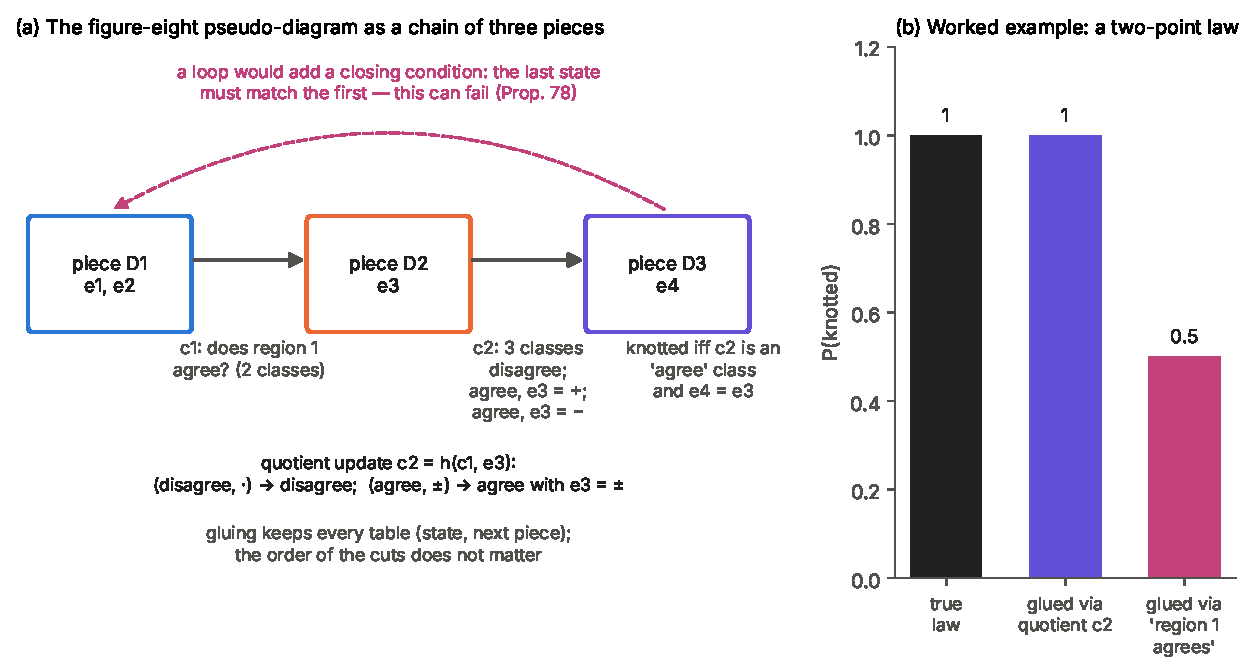
\includegraphics[width=\linewidth]{fig_chainglue.pdf}
\caption{Gluing along a chain. (a) The figure-eight pseudo-diagram cut into three pieces. The state after $D_1$ records whether twist region~1 agrees ($e_1=e_2$); the state after $D_2$ adds the sign of $e_3$ when it does. Knottedness is read from the last state and $e_4$. The dashed arc is the extra condition a loop would impose. (b) The two-point law of the worked example: gluing through the quotient keeps $P(\text{knotted})=1$, gluing through ``region~1 agrees'' alone halves it.}\label{fig:chainglue}
\end{figure}

\begin{proposition}[gluing along a chain]\label{prop:chainglue}
Let $f$ be an outcome of the crossing signs, cut into pieces $D_1,\dots,D_k$ as above, with $c_0$ constant.
\begin{enumerate}
\item[(1)] The quotients are recursive: $\bar h_i$ is well defined, so the quotient at a cut is a function of the quotient at the previous cut and the piece between.
\item[(2)] The glues at different cuts commute, and applying all of them, in any order, gives the chain law. The chain law is the maximum-entropy law with the tables of $(c_{i-1},D_i)$ for every $i$, and it keeps each of those tables.
\item[(3)] If the last state $c_{k-1}$ determines the quotient at the last cut, the chain law preserves $\mathbb E_Pf$ for every $P$. Recursion then forces every state to determine the quotient at its own cut.
\item[(4)] \emph{Which coarser states are safe.} At a single cut, let $b$ be a coarsening of the quotient (a function of it). Gluing given $b$ preserves $\mathbb E_Pf$ for every law $P$ if and only if, on each class of $b$, $f$ splits as $f(x,y)=a(x)+\beta(b,y)$: within a class, two left assignments may change the outcome only by a constant that does not depend on the right side. The quotient is the case where that constant is $0$.
\item[(5)] Under such gluing, M\"obius components and Shapley values of a mechanism-indexed family are unchanged.
\end{enumerate}
\end{proposition}

\begin{proof}
(1) Suppose two left assignments $x,x'$ at cut $i-1$ give the same outcome against every right completion. Then so do $(x,d_i)$ and $(x',d_i)$ at cut $i$, since their right completions are among those of $x$ and $x'$.
(2) $G_i$ makes the two sides of cut $i$ conditionally independent given $c_i$ and keeps the tables of each side with $c_i$. Since each state is a function of the left and recursive, the glues compose to the product of conditionals $P(D_i\mid c_{i-1})$, in any order. This is the decomposable (junction-tree) form of the maximum-entropy law with those tables \cite{Lauritzen1996}; the constant $c_0$ makes the first factor $P(D_1)$. By induction the chain law keeps every table of $(c_{i-1},D_i)$, and in particular the law of every state.
(3) If $c_{k-1}$ determines the quotient, $f$ is a function of $(c_{k-1},D_k)$, whose table is kept, so $\mathbb E_Pf$ is preserved. Suppose an earlier state $c_j$ did not determine its quotient. Then two left assignments with the same $c_j$ are separated by some completion. Extending both by the same pieces up to the last cut gives the same $c_{k-1}$, by recursion, but different rows there, so $c_{k-1}$ would not determine its quotient either.
(4) If $f=a(x)+\beta(b,y)$ on each class, then $\mathbb E f=\mathbb E\,a(X)+\mathbb E\,\beta(b,Y)$, and the two terms depend only on the tables of (left, $b$) and (right, $b$), which the glue keeps. Conversely, take two left assignments $x,x'$ in one class of $b$, two right assignments $y,y'$, and the law with mass $\tfrac12$ on each of $(x,y)$ and $(x',y')$. The glue spreads it evenly over the four pairs, so preservation requires $f(x,y)+f(x',y')=f(x,y')+f(x',y)$. Hence $f(x,y)-f(x',y)$ does not depend on $y$, which is the splitting.
(5) As in \cref{prop:boundary}.
\end{proof}

Part~(4) answers the question of necessity exactly. The quotient is always enough. A coarser memo is enough only for outcomes with no interaction between the two sides inside a merged class; additive outcomes, such as the writhe, are the extreme case, and need no memo at all. For a chain the same test applies at each cut, with the left law itself glued from the earlier cuts. CH6 confirms the criterion on every coarsening of the last state for knottedness and the writhe, and on $30$ random outcomes, $40$ laws each.

\paragraph{A worked example.} Cut the figure-eight into $D_1=\{e_1,e_2\}$, $D_2=\{e_3\}$ and $D_3=\{e_4\}$ (\cref{fig:chainglue}). Knottedness is $\tfrac14(1+e_1e_2)(1+e_3e_4)$: twist region~1 must agree, and $e_4$ must equal $e_3$. The first memo has two classes, ``region~1 agrees'' and ``it does not''. The second has three: disagree; agree with $e_3=+$; agree with $e_3=-$. Now take the law with probability $\tfrac12$ on $(e_1,e_2,e_3,e_4)=(+,+,+,+)$ and $\tfrac12$ on $(+,+,-,-)$. Both outcomes are knotted, so $P(\text{knotted})=1$. Gluing through the three-class memo returns the same law, so it keeps $P(\text{knotted})=1$. Gluing through ``region~1 agrees'' alone puts both points in one class and spreads the mass over the four pairs $(e_3,e_4)$, of which two are knotted, so $P(\text{knotted})=\tfrac12$. The two points differ on the left by $e_3$, and $e_3$ interacts with $e_4$, so part~(4) predicts the loss.

Along the figure-eight cut into its four single crossings, the quotient states have sizes $2$, $2$ and $3$. Over random laws, dropping $e_3$ from the last state, while keeping the earlier ones, changes $P(\text{knotted})$ by up to $0.25$ and changes the attribution. Combinatorial gluing, which only matches boundary configurations, is order-independent on any diagram. Probabilistic gluing is order-independent on chains because they are decomposable. CH1--CH6 check recursion, commutation in every order, the maximum-entropy property, preservation and its failure, attribution, the loop below, and the coarsening criterion.

\begin{remark}[loops]\label{rem:chainloop}
On a chain information only flows forward, and no state has to agree with anything at the far end. Closing the chain into a loop adds that condition: the last state must match the first. Compatibility of every pair of neighbours does not imply it. \Cref{prop:twist} gives an exact case: on a cycle of perfectly correlated or anticorrelated pairs, a global law exists if and only if the product of the signs is $+1$, and removing any one link opens the cycle into a path, which always glues. With $n=3$ this is the impossible pair data of the pseudo-trefoil above. The sign twist is proved here only for this cycle-sign model. Which obstructions can arise for general loops of tangles is open.
\end{remark}

\begin{remark}[automata and tangles]\label{rem:nerode}
The quotient is the Myhill--Nerode construction \cite{Nerode1958}. Read the crossing signs as a word; two prefixes are equivalent when no suffix can tell them apart; the classes are the states of the smallest automaton that computes $f$, and $\bar h_i$ is its transition. The memo of \cref{prop:chainglue} is that automaton run along the chain, with a probability law attached.

The analogy shows what the step to general tangles involves. Replace crossing assignments by tangles with a fixed boundary, and call two tangles $T,T'$ equivalent when $f(T\cup E)=f(T'\cup E)$ for every complementary tangle $E$. This equivalence is automatically compatible with composition: if $T\sim T'$ and $F$ is any tangle that can be attached, then $T\circ F\sim T'\circ F$, because every complement $E$ of $T\circ F$ makes $F\cup E$ a complement of $T$. Composition of classes is therefore well defined, and associative because it is computed on representatives. So composition is not the hard part. The hard parts are whether there are finitely many classes for each boundary, and whether they can be computed. For the Kauffman bracket the answer is a finite dimension rather than a finite number of classes: the skein relations reduce every tangle with $2n$ boundary points to a combination of the $C_n$ crossingless matchings, a Catalan number of them, so the memo is a vector in a Temperley--Lieb module of that dimension \cite{Kauffman1987}; \cref{prop:tlmemo} works this out for four ends. For knot type itself the classes are infinite already with four boundary points: the tangles of $n$ half-twists, closed by the same complement, give the torus links $T(2,n)$, which are all distinct. In the fixed-diagram setting of this section only the crossing signs vary, so the classes are always finite. That is why the construction works here, and why general tangles need an outcome, such as the bracket, whose memo stays finite-dimensional.
\end{remark}

\paragraph{Two layers.} The constructions above work on two layers at once, and it helps to keep them apart. The \emph{topological layer} is the diagram: crossings, how the strands connect, and how pieces are joined. The \emph{probabilistic layer} is a law on how the undetermined crossings resolve. Each notion has a counterpart on the other layer.
\begin{center}
\small
\begin{tabular}{p{0.42\linewidth}p{0.48\linewidth}}
\toprule
topological layer & probabilistic layer\\\midrule
crossings and strand connectivity & random resolutions of the crossings\\
boundary state of a piece & the cut state as a random variable\\
composing pieces & gluing given the cut state\\
an invariant of the closed diagram & the outcome $f$ and its expectation\\
pieces no complement can tell apart & cut states that may be merged for every law\\
\bottomrule
\end{tabular}
\end{center}
Composition on the topological layer is exact and associative whatever the shape of the diagram. Gluing on the probabilistic layer is exact on chains and can fail on loops (\cref{rem:chainloop}). In the fixed diagrams used so far the connectivity never changes; only the signs vary, so the boundary state carries signs, not connectivity. The next example lets the connectivity vary as well, through the smoothings of the Kauffman bracket, so that the memo becomes a record of how the boundary points are joined.

\paragraph{A memo that records connectivity.} Take a tangle with four ends, NW, NE, SW and SE, and build it from the tangle $[0]$ (two horizontal arcs) by adding crossings one at a time, either on the right (H, tangle addition) or at the bottom (V, tangle multiplication). These are Conway's rational tangles \cite{Conway1970}. Without crossings, the four ends can be joined in only two ways: $[0]$, which joins NW to NE and SW to SE, and $[\infty]$, which joins NW to SW and NE to SE. The bracket's skein relation replaces each crossing by a weighted sum of its two smoothings, and a closed loop by $\delta=-A^2-A^{-2}$. So the left part of the chain, whatever its crossings, is equivalent to a combination $\alpha[0]+\beta[\infty]$, with Laurent polynomials $\alpha,\beta$. That pair is the memo: the weights of the two possible connections. Adding a crossing that resolves $r=\pm1$ acts by a $2\times2$ matrix. With $a=A^{r}$,
\[
H(r)=\begin{pmatrix}a&0\\a^{-1}&a+a^{-1}\delta\end{pmatrix},\qquad V(r)=\begin{pmatrix}a+a^{-1}\delta&a^{-1}\\0&a\end{pmatrix}.
\]
Closing the four ends is a linear functional: the numerator closure (NW to NE, SW to SE) is $(\delta,1)$ and the denominator closure (NW to SW, NE to SE) is $(1,\delta)$, with the unknot normalised to $1$.

\begin{proposition}[memos in the Temperley--Lieb module]\label{prop:tlmemo}
Let a chain of crossings of types $t_1,\dots,t_k\in\{H,V\}$ resolve as $r_1,\dots,r_k$ under a law $P$, and let $f$ be the bracket of a closure of the resolved diagram.
\begin{enumerate}
\item[(1)] The memo after $i$ crossings is $v_i=M_{t_i}(r_i)\cdots M_{t_1}(r_1)\,e_0$, with $e_0$ the vector of $[0]$, and $f=n\cdot v_k$ for the closure functional $n$. It is a recursive cut state, and it is sufficient: $f$ is a function of $(v_{k-1},r_k)$. So the chain law with the memos as cut states preserves $\mathbb E_Pf$, and the law of any function of $f$, such as the indicator that the closure has the bracket of a given knot.
\item[(2)] The memo always lives in a space of dimension $2$, but the number of distinct memos, and with it the number of outcome classes, can grow with the length of the chain. Finite dimension is not finite index.
\item[(3)] If the crossings resolve independently, $\mathbb E_Pf=n\cdot\mathbb E[M_{t_k}(r_k)]\cdots\mathbb E[M_{t_1}(r_1)]\,e_0$: two numbers per cut, the expected memo, are enough. For a general law they are not.
\end{enumerate}
\end{proposition}

\begin{proof}
(1) The matrices are the skein relation applied to the new crossing: on the right, $[0]$ is the identity for addition, $[0]+[\infty]=[\infty]+[0]=[\infty]$ and $[\infty]+[\infty]=\delta[\infty]$; at the bottom the roles of $[0]$ and $[\infty]$ are exchanged. Changing the resolution of a crossing swaps its two smoothings, which swaps $A$ and $A^{-1}$. The bracket is linear in the tangle, so closing is a linear functional, and $f=n\cdot M_{t_k}(r_k)v_{k-1}$. Sufficiency then gives preservation, by \cref{prop:chainglue}(3).
(2) The dimension is that of the module spanned by $[0]$ and $[\infty]$. The growth is a computation; see below.
(3) Independence makes the expectation of the product of matrices the product of their expectations, and $f$ is linear in the product. Without independence the expectation of a product is not the product of expectations; the example below shows the difference.
\end{proof}

Part~(3) for independent crossings is the probabilistic bracket of Diamantis and Kauffman \cite{DiamantisKauffman2026}, written as a transfer matrix. Part~(2) refines \cref{rem:nerode}. For the bracket, the right notion is finite \emph{rank} rather than finite index: the memos live in a module of fixed dimension, as the states of a weighted automaton live in a vector space whose dimension is the rank of its Hankel matrix \cite{Fliess1974}. With $2n$ ends the dimension is the Catalan number $C_n$, here $C_2=2$. Along the chain $HVHVHVHV$, the completions of each cut separate any two different memos, so the outcome classes are the distinct memos. Their numbers at the seven cuts are $2,3,6,10,16,27,44$, while the dimension stays $2$. The memo also depends on the order of the crossings: one $H$ then one $V$ gives a different memo from one $V$ then one $H$. This is where connectivity enters, since an $H$ crossing and a $V$ crossing join different ends.

\paragraph{Worked example.} The chain $HHVV$, closed by the denominator closure, is a pseudo-diagram of the figure-eight knot. Of its $16$ resolutions exactly two, $(+,+,-,-)$ and $(-,-,+,+)$, give the figure-eight bracket $A^8-A^4+1-A^{-4}+A^{-8}$; we compared it with the PD-code computation behind \cref{prop:figeight}. The two are mirror images, as they should be, since the figure-eight is its own mirror image. So here the event that the closure is the figure-eight is a function of $f$. Put probability $\tfrac12$ on each.
\begin{itemize}
\item The true law gives $P(\text{figure-eight})=1$ and $\mathbb E f=\langle 4_1\rangle$.
\item Gluing along the chain with the memos as cut states keeps both.
\item Gluing at the middle cut with a state that records only whether crossings $1$ and $2$ agree merges $(+,+)$ and $(-,-)$, whose memos differ. It gives $P(\text{figure-eight})=\tfrac12$.
\item Propagating the expected memo, as if the four crossings were independent with probability $\tfrac12$ each, gives $P(\text{figure-eight})=\tfrac18$: two of the sixteen resolutions.
\end{itemize}
So the topological layer composes the two-dimensional memos exactly, and the probabilistic layer needs the joint law of the memo with the next crossing. Over $40$ random laws the memo chain law reproduces $\mathbb E f$ to rounding error, while independence and the agreement-only state miss it by up to $3.3$ and $1.5$ (at $A=0.7$ and $1.3$). TM1--TM6 check the transfer matrices against a direct state sum over all smoothings, Reidemeister~II, the figure-eight, the growth of the classes, the independent case exactly, and the example.


\paragraph{The cut quotient by elimination.} \Cref{prop:boundary} finds the classes of a cut by comparing outcomes against every completion. There is an algebraic way to get the same classes, and it says how expensive each cut is. Write the outcome as a polynomial in the crossing signs, reduced by $e_i^2=1$, and collect it by the monomials $m(y)$ of the right-hand signs:
\[
f(x,y)=\sum_m a_m(x)\,m(y).
\]
The coefficients $a_m$ are polynomials in the left-hand signs. The right-hand monomials are linearly independent functions, so two left assignments give the same outcome against every completion exactly when they have the same coefficient vector $(a_m(x))_m$. The classes are the fibres of this coefficient map, and the cut needs to carry only the point of its image.

\begin{proposition}[the cut quotient as an elimination ideal]\label{prop:elimquot}
Let $I=\langle x_i^2-1\ (i\in S),\ u_m-a_m(x)\rangle$ and let $I_u=I\cap\mathbb Q[u]$ be its elimination ideal, the part of a lexicographic Gr\"obner basis that is free of the left variables.
\begin{enumerate}
\item[(1)] The zeros of $I_u$ are the distinct coefficient vectors, one for each class of the cut, and $I_u$ is their full vanishing ideal.
\item[(2)] The number of classes is the degree of $I_u$, the number of standard monomials of any Gr\"obner basis of it.
\item[(3)] The linear span of the coefficient vectors can be smaller than the number of classes. The rank and the number of classes answer different questions, as in \cref{prop:tlmemo}.
\end{enumerate}
\end{proposition}

\begin{proof}
$I$ is the vanishing ideal of the finite set of points $(x,a(x))$, $x\in\{\pm1\}^S$, since $x_i^2-1$ cut out the cube with multiplicity one and $u_m-a_m(x)$ cut out the graph. Eliminating $x$ projects a finite set of points, and the elimination ideal of the vanishing ideal of a finite set is the vanishing ideal of its projection \cite{CoxLittleOShea2015}. This gives (1). A zero-dimensional radical ideal has as many points as standard monomials, which gives (2). For (3), see the example below.
\end{proof}

For the figure-eight at the cut $\{1,2\}\,|\,\{3,4\}$ the coefficient map is $x\mapsto\tfrac14(1+e_1e_2)(1,1)$, and elimination leaves $u_0=u_1$, $u_1^2=u_1/2$: two points, the agree and disagree classes, and a span of rank $1$. At the cut $\{1,3\}\,|\,\{2,4\}$ the map is $x\mapsto\tfrac14(e_1e_3,e_1,e_3,1)$, whose image has four points: nothing can be merged. After crossings $1,2,3$ the degree is $3$ and the rank $2$. The degrees along the chain, $2,2,3$, are the state sizes of \cref{prop:chainglue}, and for the bracket memo of \cref{prop:tlmemo} along $HVHV$ they are $2,3,6$.

\paragraph{Components of a decision path.} Read the crossings as the switches of a decision path in the order they happen. The left side of a cut is the decision maker's private past, and the right side is everything still to come. The degree of $I_u$ is then the number of things the ledger must be able to tell apart about the past, and the degree of the mirror ideal on the right is the same for the future. That makes the degree a price for cutting the path at that point, and it suggests what the \emph{components} of a path are: the stretches between cheap cuts. They need not be the stretches between switches. If the four switches of the figure-eight outcome happen in the order $1,2,3,4$, the cheapest cut is after the second switch, at $(2,2)$ classes, and it separates the two twist regions. If they happen in the order $1,3,2,4$, the same cut costs $(4,4)$: the two regions interleave in time, and no cut in the middle separates them. Which switches a ledger must watch is read off the same expansion: those that appear in a monomial spanning the cut.

Gr\"obner bases are exact for this layer, where each switch resolves $\pm1$. Once the monitored quantities are continuous and their identified intervals enter, the constraints are inequalities. Elimination over the complex numbers does not see them. The projections are then polytope projections, which the linear programs of \cref{sec:ledgerdm} compute, and the question ``for every future'' becomes real quantifier elimination. Gr\"obner methods are used in knot theory for other purposes: Gr\"obner--Shirshov bases give normal forms of braid words \cite{BokutChen2014,Bokut2008}, which could normalise the braid words of a crossing log, and Gr\"obner bases of elementary and Fitting ideals give computable invariants of a fixed knot or link \cite{CransHenrichNelson2013,NosakaShimizu2026}. Here elimination is used for something different: to compute what a cut must carry. EQ1--EQ5 check the degrees against the classes of \cref{prop:boundary} on every cut, for knottedness, the writhe and $20$ random outcomes, the rank, the chain and memo degrees, and the two orders of the decision path.

\paragraph{What this lays down for knots traced by trajectories.} The example has the shape the trajectory question needs. The undetermined switches of a closed decision path are the pre-crossings. The data about them, which switches are identified and how often each resolves one way across histories, are the observed tables. The way they resolve jointly lies in a fibre. A topological property of the closed path is then determined by the data exactly when its Walsh terms are covered. Which terms these are depends on the diagram: for the pseudo-trefoil, knottedness needs pairs of switches, and for the figure-eight diagram it needs all four switches together. A figure-eight can arise only when at least three quantities are monitored, since two strands close only to torus knots (\cref{sec:ledgerdm}). Two things are still missing. First, a crossing needs an over/under sign, which needs a coordinate beyond the order of two numbers (\cref{rem:topology}). Second, larger diagrams need composition. \Cref{prop:cutglue} does the simplest case, two pieces and one cut state; general tangles, with their boundary connectivity, remain to be done. PK1--PK5 check the polynomials, the expansions, the criterion on $540$ random interior cases, the example and the impossible pair data.


\subsection{Snapshots and a private decision ledger}\label{sec:ledgerdm}
The previous subsections give a decision maker several instruments: fibres, value of information, contextuality tests, poisoning
radii, holonomy, Bloch coordinates and pseudo-knots. This subsection puts them in one setting. It is meant for a decision maker who
works alone against an environment that others can write into. It makes no new claims; it fixes vocabulary and says which piece
comes from where.

\paragraph{Roles.} Four things are kept apart.
\begin{itemize}
\item \emph{The environment} is the true joint law $P^*_t$, which may drift. Nobody sees it directly.
\item \emph{The data} are tables dumped into a shared store, snapshot by snapshot. Most come from the environment, some from actors.
\item \emph{Actors} write into the store. A \emph{steering} actor adds data that some single world could have produced, aimed at moving a
decision. A \emph{confusing} actor adds data that no single world could produce, for example tables that are each plausible but that
do not glue.
\item \emph{The decision maker} reads the store, decides, and keeps a private record of how each decision was reached.
\end{itemize}

\paragraph{The snapshot and the ledger.} At each snapshot $t$ the store defines a public information state, the pooled tables of
the observed contexts. From it the decision maker derives a private \emph{ledger}:
\begin{enumerate}
\item the consistency residual, the least change that makes the tables glue, and the fibre $J_t$ of the repaired tables (\cref{sec:cycle,prop:twist});
\item the selected law and the rule that selected it, together with the identified interval $[L,U]$ of each monitored quantity and the regret $R$ (\cref{prop:decisions});
\item the action, and the value of information of any signal under consideration, with its envelope (\cref{thm:determination});
\item the history of selections and its holonomy against a flat rule (\cref{prop:holbound,prop:flat});
\item a crossing log: each switch of the action, marked \emph{classical} if the data fix it on both sides and as a \emph{pre-crossing} if it is made while $R>0$ (\cref{rem:topology}); and each exchange of order between two monitored quantities, marked the same way;
\item for each binary decision, a point of the \emph{decision-state ball} defined below, which records the selected probability and how well the data identify it.
\end{enumerate}
Actors see the actions and their own dumps, not the ledger. Privacy here means only that this observation is many-to-one: many ledgers
give the same actions. It does not mean the ledger cannot be inferred.

\paragraph{What the two kinds of interference do.} The ledger's instruments separate them, in principle.
\begin{itemize}
\item Confusion raises the consistency residual. When the bogus tables are correlated around a cycle in the twisted pattern, \cref{prop:twist} says where the obstruction lies.
\item Steering need not raise the residual at all. A consistent edit moves the data inside the noncontextual set, and the cheapest
flips do exactly that (route~A of \cref{ex:stages}). Its trace is private: the decision changes, and in the ledger the change is a
pre-crossing.
\end{itemize}
Whether this separation holds in a concrete stream, and whether the crossing log warns before a steered change, are empirical
questions. Study~19 tested them in a synthetic stream, under a plan frozen before any run (\texttt{PREREG\_study19\_v3.md}; results in \texttt{RESULTS\_study19.md}). Steering worked and was not detected: the decision switched in $29$ of $30$ runs, and the residual alarm fired in one. Everything else failed. The confusion adversary, a $20\%$ share of PR-box tables, never left the noncontextual set, so it was not detected (H1). The residual threshold gave false alarms in $53\%$ of clean runs (H2). And the crossing log gave no warning beyond the decision margin, the regret $R$ or the viability share $q^*$ (H5). A diagnostic shows why. Every monitored quantity in that world was a pair never observed together, so nothing was ever identified: every switch and crossing was a pre-crossing, and the private score merely counted crossings. The ledger can discriminate only where identification varies over time. That is the condition a follow-up study has to build in. Study~20 built it in, with an aimed confusion adversary, run-level thresholds and two mechanisms: an extra context and a signal (\texttt{RESULTS\_study20.md}). Confusion was detected in every run, with false alarms in $13\%$ of clean runs. Steering switched the decision in every run and was not detected. The two mechanisms interacted as \cref{thm:determination} predicts. Observing $(A_0,A_1)$ removed all unidentification from the plain decision ($0.89\to0$), but little from the rule that consults $B_0$ ($0.98\to0.92$), which needs the triple $(A_0,A_1,B_0)$. The warning hypotheses could not be tested, because the decision was identified in only about $10\%$ of snapshots, below the pre-registered validity floor. A diagnostic also showed why the pre-crossing flag cannot help. The selected value always lies in its identified interval, so a switch, or an exchange of two strands, passes through an unidentified state by continuity. ``Made while $R>0$'' is therefore true of almost every switch. A pre-crossing worth recording has to compare selection rules instead: it should ask whether another admissible law in the fibre would not have switched in the same stretch.

\paragraph{The decision-state ball.} For a binary decision with selected probability $v$ and identified interval $[L,U]$, put $w=U-L$, $z=1-2v$ and
\[
\mathbf r=\big((1-w)\sqrt{1-z^2}\cos\phi,\ (1-w)\sqrt{1-z^2}\sin\phi,\ z\big).
\]
Then $|\mathbf r|^2=z^2+(1-z^2)(1-w)^2\le1$, so $\mathbf r$ lies in the unit ball. An identified decision ($w=0$) lies on the sphere, and a completely unidentified one ($w=1$) lies on the vertical axis. The height is the selected probability, as on the Bloch sphere. Identification plays the role that coherence plays for a qubit. The simpler choice of radius $1-w$ with height $1-2v$ is not available, since it can violate $|z|\le1-w$ (for instance $v=0.9$ with $[L,U]=[0,0.9]$). We claim only this embedding, not any quantum meaning. The longitude $\phi$ is a free choice, and two candidates are kept apart:
\begin{itemize}
\item $\theta^{\rm cycle}$, a phase within a recurrent cycle of the stream;
\item $\theta^{\rm sel}$, the holonomy of the decision maker's rule against the flat maximum-entropy rule (\cref{prop:flat}).
\end{itemize}
Neither is shown to be a geometric (Berry) phase. Every decision functional of the note ignores $\phi$ (\cref{prop:fisher}(1)), so a longitude could matter only through a phase-sensitive decision functional, which the note does not construct.

\paragraph{Braids from the crossing log.} With $k$ monitored quantities, each is a strand in (time, value, identification radius). In the projection to (time, value), an exchange of two adjacent strands is a crossing $\sigma_i^{\pm1}$. Its sign is read from oriented data: a crossing is positive when the rising strand is the one with the larger identification radius, so that it passes in front. Time is discrete, exact ties are broken by a fixed order, and strands are never created or removed. The crossing log is then a braid word in $B_k$, and its pre-crossings make it a pseudo-braid.

The number of strands limits what a closed stretch can produce. With two monitored quantities the braid group is $B_2\cong\mathbb Z$, so closures are only the torus links and knots $T(2,m)$. The pseudo-trefoil of \cref{prop:pseudoknot} is of this kind. The figure-eight knot has braid index $3$; it is the closure of $(\sigma_1\sigma_2^{-1})^2$. So \cref{prop:figeight} applies to the ledger only when at least three quantities are monitored.

\begin{center}\small
\begin{tabular}{p{0.42\linewidth}p{0.5\linewidth}}
\toprule
already in the note & new here\\\midrule
fibres, identified intervals, regret, value of information and its determination; contextuality, the sign twist; poisoning radii and route~A; histories, holonomy and flatness; Bloch spheres for example~A; pseudo-trefoil and figure-eight identification & the roles and the private ledger; the observation map and its many-to-one reading of privacy; the crossing log of a decision stream as a braid word in $B_k$, with signs from the identification radius; the decision-state ball (selection as height, identification as coherence); the hypotheses of Study~19\\
\bottomrule
\end{tabular}
\end{center}

\paragraph{Status of this direction.} The pieces have different standing, and should be read that way.
\begin{itemize}
\item \emph{Established:} which topological properties crossing data determine, by Walsh degree (\cref{prop:pseudoknot,prop:figeight}); the gluing of two pieces at a cut (\cref{prop:cutglue}); what a cut must carry for gluing, and attribution, not to depend on it (\cref{prop:boundary}); and its extension to chains of pieces (\cref{prop:chainglue}).
\item \emph{Exact in restricted examples:} the three Bloch spheres of example A (\cref{prop:bloch}). The holonomy groups of B and C are numerical observations.
\item \emph{Proposed:} the private ledger, braids from decision streams, and the decision-state ball as a decision instrument. The warning properties were not supported by Study~19, and could not be tested in Study~20. The pre-crossing flag needs redefinition (\cref{sec:ledgerdm}).
\end{itemize}

\part{Deeper selection: \texorpdfstring{$2\times4$}{2 x 4} couplings}
\subsection{Beliefs under contamination}\label{sec:contam}
Suppose the decision maker knows that some of the tables he receives have been poisoned, but not which ones, and not by whom. In practice a saboteur rarely lies all the time. He may report honestly for weeks and lie only when a decision he cares about comes near; he may hold a report back, or refuse an inspection; and if his lie produces a contradiction, he may persuade another source to change its story so that the contradiction disappears. This subsection builds a model of that situation from the decision maker's side. Everything in it is computed from what he has actually received, together with his own record of what was withheld or refused. The true law is used only afterwards, to score how well he did.

Three conclusions come out of the analysis, and it helps to state them first. A decision maker can be misled even when everything he holds is perfectly consistent. How much room a saboteur has depends on the decision in question, not only on the saboteur, so trust cannot be summarised by one score per source. And keeping the full history of reports can expose what a snapshot of the current reports hides.

At each step the decision maker works through a short cycle. He re-reads everything he has under each hypothesis about whom to trust, without deleting anything. Where the data he trusts cannot all be true, he lists the ways they could be repaired. He then asks whether his decision would come out the same under every repair he considers possible. If it would, he acts. If not, he buys the inspection that most reduces what an adversary could still do to that decision.

\paragraph{Belief as a presheaf.} Call each report a \emph{cell}: a source, a context and a time, together with the table reported. For a set $S$ of cells he chooses to trust, let $\mathcal J_t(S)$ be the fibre, the set of joint laws whose marginals agree with the tables in $S$. His belief at time $t$ is then not a single law, and not a single fibre, but the whole assignment $S\mapsto\mathcal J_t(S)$. Trusting more cells can only rule out more laws, so $S\subseteq T$ gives $\mathcal J_t(T)\subseteq\mathcal J_t(S)$. An assignment that reverses inclusions in this way is a presheaf, here with inclusion maps between fibres. (The related presheaf of \emph{local} tables, whose maps are marginalisations, is a different object, and we do not need it.) The practical point is that isolating a suspicious source is a choice of $S$, not a deletion, so it can always be undone.

Two notions come from diagnosis. A \emph{minimal conflict} is a smallest set of cells whose fibre is empty: these reports cannot all be true, but every proper subset of them can. An \emph{explanation} is a set $H$ of cells whose removal leaves a non-empty fibre $\mathcal J_t(\mathcal U_t\setminus H)$. Because a set with an empty fibre keeps that property when cells are added, the explanations are exactly the sets that meet every minimal conflict, as in Reiter's theory of diagnosis \cite{Reiter1987}. The cells that were actually corrupted always form an explanation, but not necessarily a minimal one, and this matters below.

\begin{proposition}[conflicts, exposure and robust viability]\label{prop:contam}
Let $\mathcal U$ be a finite set of cells with exact tables. Uncorrupted cells report the true marginals; corrupted cells may report anything.
\begin{enumerate}
\item[(1)] Suppose the contexts of a set $S$ form an acyclic hypergraph, meaning that they can be arranged in a join tree (equivalently, the GYO reduction, which repeatedly deletes variables that occur in only one context and contexts contained in another, removes all of them). Then $\mathcal J(S)$ is empty exactly when two overlapping cells of $S$ disagree on the variables they share. In particular, on such a family every minimal conflict is a pair of overlapping cells, a cell that overlaps no other cell is in no conflict, and a conflict among three or more cells requires a cycle of contexts.
\item[(2)] Let $\mathcal E_k$ be the set of all explanations with at most $k$ cells. If an action is optimal for every law in $\mathcal J(\mathcal U\setminus H)$, for every $H\in\mathcal E_k$, and the corrupted cells number at most $k$, then the action is among the optimal actions under the true law.
\end{enumerate}
\end{proposition}

\begin{proof}
(1) On an acyclic family, tables that agree pairwise on their overlaps always come from a common joint law; this is Vorob'ev's theorem \cite{Vorobev1962}. The converse is immediate. A minimal conflict on such a family therefore contains a disagreeing pair, and by minimality it is that pair. A cell with no overlaps can disagree with nothing. (2) The corrupted set is itself an explanation of size at most $k$, so the true law lies in one of the fibres on which the action was checked.
\end{proof}

Part~(1) distinguishes two ways in which a report can be caught. It has \emph{overlap exposure} if it shares a variable with another report, so that a neighbour can contradict it directly. It has \emph{cycle exposure} if it survives the GYO reduction, so that a closed loop of contexts can reveal a contradiction that no single overlap shows. These are different. Three pair contexts sharing one variable all overlap one another, yet together they are acyclic, and any conflict among them is a pair. The statement also needs exact tables: when small discrepancies are tolerated, tables that nearly agree in pairs need not glue. In the examples below every source overlaps its neighbours from the start, so what a saboteur avoids is cycle exposure, by staying where no loop has yet been closed. An inspection, from this point of view, is a new context that closes one.

\paragraph{The algebra of coherence.} Whether a set of reports is coherent, meaning that some joint law reproduces all of them, can be examined at several levels, and each has its own algebra. The cheapest is a sign test. Multiply the agreement signs of the reports around a cycle of contexts; if the product is $-1$, no global law exists (\cref{prop:twist}). This is the cohomological obstruction studied by Abramsky and Brandenburger \cite{AbramskyBrandenburger2011}. It is local and easy to compute, but it only sees all-or-nothing contradictions. At the linear level, the marginal map $M$ sends a joint law to its tables. A change in the data that stays in the image of $M$ simply moves to another coherent family and cannot be detected; a change that leaves the image is what the residual measures. A decision functional is pinned down by the data when it lies in the row space of the observed contexts, which is the Walsh criterion met earlier. Positivity adds the last ingredient. Probabilities cannot be negative, so coherence is the feasibility of a linear program, and when the reports are incoherent, Farkas' lemma provides a certificate \cite{Schrijver1986}: an explicit inequality that the reported tables violate. The lattice of cell sets then organises these certificates into minimal conflicts and explanations. The updates themselves compose but cannot in general be undone, so they form a monoid rather than a group; groups appear only where something is invertible, as with the signs around a cycle.

\paragraph{Tamper budgets.} Fix a decision functional $g(p)=a^\top p$, and suppose a coalition controls the reports in a set $C$ of cells while the remaining cells, $H$, are honest. Write $\mathcal P_H$ for the honest fibre and $I_H(g)=[\min_{\mathcal P_H}g,\max_{\mathcal P_H}g]$ for the range of $g$ over it.

\begin{proposition}[tamper budgets]\label{prop:tamper}
Suppose $\mathcal P_H$ is non-empty, and that the coalition can coordinate freely: it may report the tables $M_Cp$ of any law $p$ in $\mathcal P_H$, or anything else. (A coalition that cannot communicate freely, or cannot report arbitrary tables, may be able to do less.)
\begin{enumerate}
\item[(i)] Every coherent report by the coalition leaves the decision maker with a range of $g$ inside $I_H(g)$, and every value in $I_H(g)$ can be made compatible with some coherent report. So $I_H(g)$ is exactly what the coalition can do to $g$ without being seen. We call it the coalition's \emph{tamper budget} for $g$. If the honest cells report the true law $p^\star$, the budget splits into an upward part $\max_{\mathcal P_H}g-g(p^\star)$ and a downward part $g(p^\star)-\min_{\mathcal P_H}g$. If $I_H(g)$ lies entirely on one side of a threshold, no coherent report can change the threshold decision, and the coalition can change it only by producing a contradiction.
\item[(ii)] The contradiction forced by a report $z_C$ can be measured by $\rho_C(z_C)=\min_{p\in\mathcal P_H}\lVert M_Cp-z_C\rVert_1$, which is a linear program and vanishes exactly for coherent reports. When it is positive, a Farkas certificate exists, and it may involve cells far from the ones the coalition controls.
\item[(iii)] If the decision maker knows only that at most $k$ cells are corrupted, the values of $g$ compatible with some admissible repair form the union $\bigcup_{H\in\mathcal E_k}I_{\mathcal U\setminus H}(g)$. Under the assumptions of \cref{prop:contam}(2) this union contains the true value. It may have gaps, so it should not be replaced by the smallest interval containing it.
\end{enumerate}
\end{proposition}

\begin{proof}
(i) A coherent report leaves a fibre inside $\mathcal P_H$, so the range it allows lies in $I_H(g)$; conversely, the report $M_Cp$ is reproduced by $p$ itself. If $I_H(g)$ lies on one side of the threshold, so does every law the decision maker could select. (ii) Write the $\ell^1$ distance with slack variables. (iii) As in \cref{prop:contam}(2).
\end{proof}

Part~(i) is about which values can be made \emph{compatible} with the reports. Which value a particular decision rule then \emph{selects}, whether the maximum-entropy law or the midpoint of a range, is a separate matter, taken up in \cref{prop:miscal}(D). The proposition explains how a source can look perfectly reliable. Coherence is a property of the reports alone, while the budget depends on the reports and on the decision. On a decision whose honest range is a single point, the source has no room to deviate; on decisions it does not care about, it has no reason to; and on the decision it wants to tilt, it moves within its budget and nothing is seen.

\paragraph{A sign example.} Five sources report the sign of $X_iX_{i+1}$ around a five-cycle, and the true signs are all $+1$. Suppose the first four reports arrive with $s_1=-1$ and the others $+1$. These four contexts form a path, and the reports are coherent, so the false sign cannot yet be seen. When a fifth, independent report with $s_5=+1$ closes the cycle, the product of the signs is $-1$, and the five cells together form a single minimal conflict. Each single cell is a minimal explanation. The decision maker now knows that something is wrong but cannot tell what. If $S_3$ is then persuaded to report $s_3=-1$, the product returns to $+1$ and the reports are coherent again, and still false. The only trace left is in the history: if the earlier report of $S_3$ is kept as a separate cell, the two reports of $S_3$ contradict each other. A set of reports can become more coherent while becoming less true, which is why the history has to be kept.

\begin{figure}[!htbp]\centering
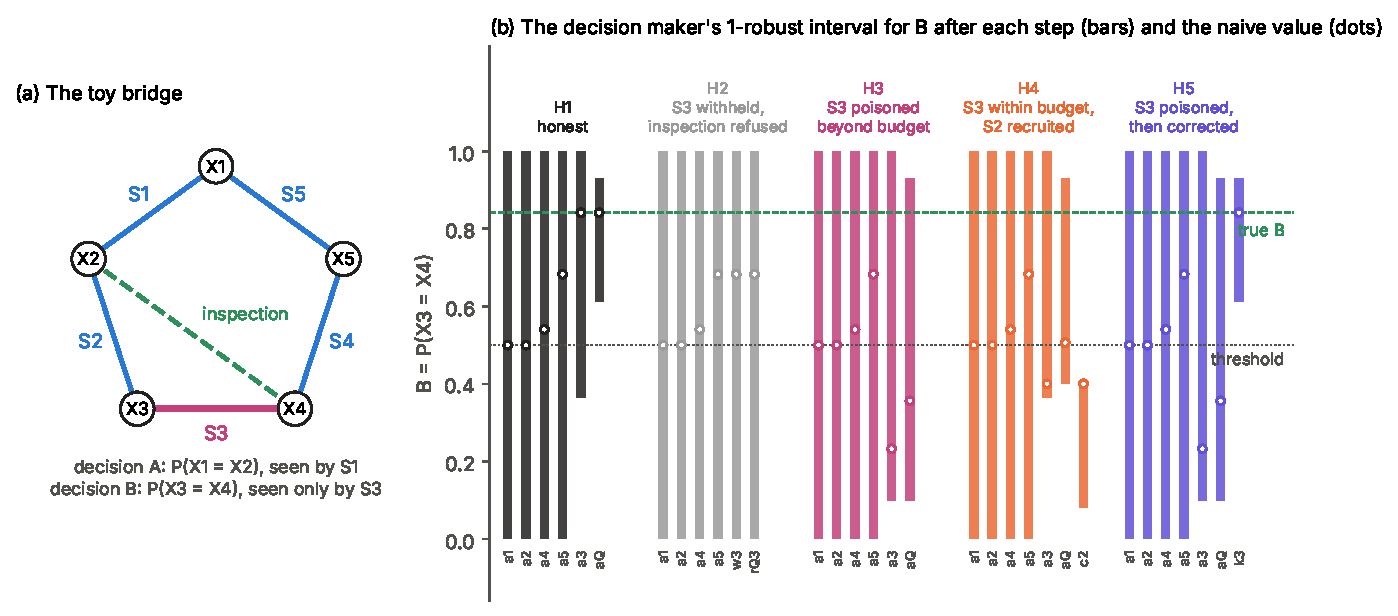
\includegraphics[width=\linewidth]{fig_bridge.pdf}
\caption{The bridge example. (a) Five binary variables on a cycle, one source on each edge, and the inspection the decision maker buys. Decision $A$ is seen directly by $S_1$, decision $B$ only by $S_3$. (b) Five histories starting from the same law. The bars show the decision maker's $1$-robust range for $B$ after each step, and the dots show his naive estimate, the midpoint of the least-incoherent fibre. The true value of $B$ (dashed) is shown only for comparison; he never sees it. Labels: $a_i$ arrival of $S_i$; $a_Q$ the inspection; $w_3$ a withheld report; $r_{Q3}$ a refused inspection; $c_2$ a recruited repair; $k_3$ a correction.}\label{fig:bridge}
\end{figure}

\paragraph{The bridge example.} Keep the five-cycle, now with a joint law of Ising type, two decisions $A=P(X_1=X_2)$ and $B=P(X_3=X_4)$, threshold $\tfrac12$, and true values $A=B=0.841$ (\cref{fig:bridge}). Consider $S_3$ acting alone. Its budget for $A$ is a single point, because $S_1$ reports $A$ directly. Its budget for $B$ is $[0.365,1]$, which contains the threshold, so $S_3$ can reverse the decision on $B$ without being seen. A report of agreement $0.40$ produces no contradiction at all. A report of $0.10$ produces a residual of $0.53$, and the Farkas certificate involves all five cells, not just the neighbours of $S_3$. Of the five possible inspections, two (the chords $(X_2,X_4)$ and $(X_3,X_5)$) shrink the worst-case range for $B$ to $[0.613,0.930]$, above the threshold, while the other three leave it straddling it.

The budget just described is relative to what the decision maker holds now. It is also useful to ask what remains after every inspection he could still buy. With all five chords inspected honestly, $S_3$'s range for $B$ is $[0.613,0.930]$, entirely above the threshold. A lie that fits the current budget but not this \emph{durable} one is undetectable now and detectable later, and this is how the inspection exposes $S_3$ in the fourth history below.

The five histories all start from the same law, and in each the reports of $S_1$, $S_2$, $S_4$ and $S_5$ arrive first. In $H_1$ everyone is honest. In $H_2$ the report of $S_3$ never arrives, and the decision maker's request to inspect that context is refused. In $H_3$, $S_3$ reports a value far outside its budget. In $H_4$ it stays within its budget, the inspection then exposes it, and $S_2$ is recruited to change its report so that the contradiction disappears. In $H_5$, $S_3$ lies and later corrects itself, so the history ends with the same tables as $H_1$. The naive decision is wrong in $H_3$ and $H_4$. The $1$-robust rule, which considers every explanation with at most one cell, is either right or says ``investigate'' whenever at most one cell is corrupted. Recruitment defeats it. After $S_2$'s change there are two corrupted cells, the false world is coherent, it is the only explanation with a single cell, and the rule rejects. The simplest explanation is now the saboteurs' own. What helps is again the history. If $S_2$'s first report is kept as a separate cell, the two reports of $S_2$ contradict each other, and with $k=2$ the rule returns to ``investigate''. The current reports being compatible does not mean the history is consistent. A source that changes its report on a context immediately after an inspection has exposed a conflict on that context's cycle is the typical sign of recruitment. It is evidence, not proof: an honest correction, or a genuine change in the world, would produce the same change of report under a model in which conditions are assumed stable.

\paragraph{Missing data, and data missing on purpose.} From the tables alone, an honest gap and a deliberate one look the same. This is Rubin's distinction between data missing at random and data missing because of what they would have shown \cite{Rubin1976}. Structure still leaves a trace. The decision maker can rank every missing context $q$ by how much it would shrink his robust range, $R(q)=\mathbb E_{\mu_t}[\operatorname{width}I_t(g)-\operatorname{width}I_{t,q}(g)]$. Because a fibre is a set of laws rather than a distribution over them, the averaging measure $\mu_t$ has to be declared. Here it is the distribution of the solution of a linear program over the fibre with a random Gaussian objective, and we report the smallest and largest values over the draws as well as the mean. In $H_2$ the withheld context $(X_3,X_4)$ comes first among the six missing contexts on all three counts, with a reduction of $1$ for every draw, and every other context scores $0$. The inspection that was refused is the same context. Honest gaps have no reason to follow this ranking, while deliberate ones keep removing whatever is at its top. A refusal is itself information about how data become available. Reading it as evidence of sabotage, though, requires an assumption, that honest sources rarely refuse decision-critical inspections, or a test of that assumption. It does not establish intent.

\paragraph{Events, braids and shadows.} Three further ways of describing these histories can be compared on the example.

The first is a record of events. The state is a pair $(R,W)$, where $R$ assigns to each report key, a pair of source and context, the table currently reported, and $W$ lists what was withheld or refused. An event inserts or replaces a report under one key, or adds to $W$. Two events are independent when performing them in either order gives the same state. This holds for events on different keys, which here have no side effects on each other. Events on the same key are dependent unless their particular effects happen to commute, since replacing a table by $u$ and then by $v$ is not the same as the reverse. A history is then an element of a trace monoid, the algebraic structure in which independent letters may be swapped, and its Cartier--Foata normal form groups the events into layers of mutually independent ones \cite{CartierFoata1969,DiekertRozenberg1995}. Each letter carries the content of its report, so the poisoned report of $H_3$ is a different letter from the honest one in $H_1$. What the decision maker could infer when a report arrived is kept alongside the letter rather than inside it: whether the current reports were still compatible, whether every report ever received still was, and whether the report revised an earlier one under the same key. These annotations depend on the order of arrival. In $H_4$, for example, the contradiction is attached to the inspection only because the inspection came second. Marks that do not depend on order can be read off the complete history instead. In $H_4$ the reports lying in some minimal conflict are those of $S_2$, $S_3$ and the inspection, which clears $S_1$, $S_4$ and $S_5$. The recruited change in $H_4$ and the honest correction in $H_5$ look the same: both arrive compatible with the current reports, inconsistent with the history, and as revisions. A second layer of letters records the changes of the robust decision on $B$. For these, independence cannot be assumed from the labels; it is checked directly by recomputing the decision with and without the neighbouring event. Since the check uses only the states the history actually visits, the resulting independence holds along that history and not necessarily in general. In every history, each decision letter comes immediately after the events it depends on. The record says what the decision maker saw and inferred, not whether any source was honest.

The second description is a braid. Its strands are the five readings of $B$ obtained by trusting everyone except $S_i$, for $i=1,\dots,5$; all five are numbers on the same scale. A crossing is a moment at which two readings change order, and by a rule fixed in advance the strand with the wider range passes over. Running a history forward and then back along a fixed replay of its final tables gives a closed loop, whose braid can be tested for triviality with Artin's faithful action on the free group \cite{Artin1947}. The reordered honest history has the same braid as the original. But the loop of the honest history $H_1$ is non-trivial, while that of the recruited $H_4$ is trivial, so in this example the braid does not indicate sabotage.

The third description follows the decision maker's state as a single curve through six coordinates: the value of the best available inspection, the residual, the width of the robust range, the naive estimate, how far the tables have drifted since first reported, and the number of withheld reports and refusals. An embedded closed curve in four or more dimensions can always be untied \cite{Rolfsen1976}, so such a curve has no knot type as a whole; and a trajectory that returns to a state it has visited is not embedded at all, its self-intersections being information in their own right. Knot types therefore live in the three-coordinate shadows of the curve, one for each choice of three coordinates, and different shadows can carry different knots. In three dimensions the knot type does not change when a coordinate is rescaled or reparametrised monotonically, so units do not matter, while reversing a coordinate gives the mirror image. Many shadows touch themselves, because the history revisits states, and at such a point the three chosen coordinates cannot decide which strand passes over; the remaining coordinates can. These are pseudo-crossings, resolved by another view of the same history. In the example, none of the $120$ shadows is knotted: $77$ touch themselves, $37$ are unknotted and $6$ are degenerate.

What the decision maker can actually use from this subsection is fairly concrete. He can compute, for each decision, the budget of each possible coalition, and so knows which decisions can be tilted without trace and by whom. The robust rule with its third option, ``investigate'', never accepted or rejected wrongly as long as the number of corrupted cells stayed within its assumption. The ranking of inspections chose one that both settled $B$ and exposed the lie that had stayed within budget. Keeping every source's earlier reports turned recruitment into a visible contradiction, the ranking of missing contexts exposed the withholding, and the record of events, with its contents, documents what happened. The braid and shadow descriptions are pictures. In this example they did not separate honest from manipulated histories, and they are reported as computed, without searching afterwards for a more favourable projection.

To summarise the status of this subsection: \cref{prop:contam,prop:tamper} are proved; the bridge example, its inspections and the ranking of missing reports are computed; the difference between current compatibility and historical consistency is shown on the example; and the braid and shadow descriptions remain exploratory, with no detector established.

\paragraph{Study 21: do braids and shadows predict more than the record?} Regret scores a decision, while a braid or a knot describes the history that led to it, so any link between them has to be predictive. And because the braid is computed from the history, it can at best improve on a \emph{summary} of that history, never on the history itself. Study 21, pre-registered, frozen and run once (\texttt{synthetic\_sections/RESULTS\_study21.md}), tested this directly. It drew $360$ random versions of the bridge, with random couplings, a random target source, six scenarios ranging from honest reporting to recruitment, random orders of arrival, and an inspection chosen by the decision maker. Just before the inspection it computed three groups of features. The baseline consisted of counts from the event record, the residual, the width of the robust range, the position of the threshold, the naive estimate, the size of the smallest explanation, and the decision maker's own worst-case regret over his robust range. All of these use only his information; realised regret, which uses the true law, served only as an outcome. The other two groups were the braid features and the shadow features described above.

Out of sample, the baseline predicted all three primary outcomes better than a constant: realised regret, a later contradiction, and the value of the inspection. Adding the braid and shadow features improved none of them. The mean change in loss was $-0.0001$ $[-0.0005,0.0003]$ for regret, $-0.015$ $[-0.033,0.003]$ for contradiction, and $-0.00052$ $[-0.00102,-0.000016]$ for the value of the inspection, a negligible loss. This shows no added value; it is not a demonstration of equivalence, since no margin of negligible effect was fixed in advance and the power to detect a small effect was not established. None of the $7{,}200$ shadows was knotted, and the braid loops were non-trivial in $65\%$ of honest runs, as in the example. Realised regret was largest under recruitment ($0.21$, with $90\%$ of decisions on the wrong side), followed by manipulation within the budget ($0.18$; $78\%$) and manipulation beyond it ($0.175$; $58\%$), and this cost is what the baseline already predicts. The scenarios were not matched in the size of their manipulations, so the ordering holds within this design only. Study 21 shows where the warning is not to be found, and its braid and shadow features are not reinterpreted after the event.

\subsection{Coherent miscalibration}\label{sec:miscal}
Imagine a watch whose hands move smoothly, whose gears mesh and whose display is perfectly consistent, but which someone has set three hours wrong. Nothing in it is broken; it faithfully carries out a corrupted setting. Now imagine several watches set wrong by the same person, or a single watch made to run slightly slow every day. They agree with one another perfectly, and every internal check passes. A broken watch is caught by its own mechanism; a watch that has been set wrong is not. Comparing it with a second watch helps only if someone else set the second one. A consistency check can certify that a watch is working without certifying that it shows the right time. Study~21 had already pointed in this direction: the most damaging scenario there was recruitment, the one that stays consistent.

Four properties need to be kept apart, and each is judged against something different. \emph{Coherence} asks whether the reports agree with one another, and is judged by a stated family of checks on the current reports. \emph{Calibration} asks whether they track the world, and the decision maker can judge it only against independent anchors such as his own inspections. \emph{Historical integrity} asks whether the changes in the reports can be explained, which requires a stated model of how honest reports may change. \emph{Decision stability} asks whether the decision can be pushed across its threshold, and is judged against the range left by the anchors. Exact reports of a real world are always coherent, so calibration implies coherence. The converse fails, and the gap between the two is what this subsection is about.

\paragraph{Synchronised deformations.} Divide the reports into those controlled by a coalition, $x_C$, and the rest, $h$, which remain honest. Let $\mathcal C$ be the set of report configurations that pass a stated family of consistency checks (here, that all the reports are marginals of one joint law), and let $g$ be the decision value, with threshold $\tau$. A \emph{synchronised deformation} is a continuous path $x(t)$ inside $\mathcal C$ along which the coalition's reports move together, the honest reports stay fixed, and $g$ crosses $\tau$. Two versions should be distinguished. In the first, several sources simply coordinate their reports. In the second, the reports respond to the decision maker's own decisions through some feedback rule. Both can be described in the same state space, but nothing here shows that they are the same phenomenon.

\begin{proposition}[coherent miscalibration]\label{prop:miscal}
Take the consistency checks to be ``all reports are marginals of one law'', keep $h$ fixed, and let $g$ be linear in the law.
\begin{enumerate}
\item[(A)] A path passes the checks at every moment exactly when it stays in $\mathcal C$. For fixed $h$, the configurations available to the coalition form a convex set, so the straight path between any two consistent configurations is consistent throughout.
\item[(B)] The values of $g$ the coalition can reach consistently form the interval $I_C(h)$ of $g$ over the honest fibre. This interval contains the budget of every member acting alone, because removing more reports can only enlarge the fibre.
\item[(C)] Let $a$ be anchors that the coalition cannot move, and let $I_C(h,a)$ be the range of $g$ over the laws that match both $h$ and $a$. If $\tau$ lies outside $I_C(h,a)$, no synchronised deformation consistent with the anchors can carry the decision across $\tau$. Conversely, if $\tau$ lies inside $I_C(h,a)$ and the coalition's reports determine $g$ once the others are fixed, a straight consistent path does carry it across.
\item[(D)] Let $s$ be the decision maker's selection rule, which maps consistent reports to a law, and put $v=g\circ s$. If $v$ is continuous along a consistent path $z(t)$ with $v(z(0))>\tau>v(z(1))$, then the selected value equals $\tau$ at some point of the path. For the robust rule, whose output is a range, the corresponding statement is that, wherever the ends of the range move continuously along the path, the range passes from above $\tau$, through straddling it (``investigate''), to below it.
\end{enumerate}
\end{proposition}

\begin{proof}
(A) The first statement is the definition. For convexity, a mixture of two laws that match $h$ also matches $h$, and its marginals are the mixtures of the marginals. (B) This is \cref{prop:tamper}(i) applied to the coalition, together with the fact that fibres grow as reports are removed. (C) Every consistent configuration that agrees with $h$ and $a$ comes from a law in that fibre, so its value of $g$ lies in $I_C(h,a)$. For the converse, follow the straight path from the true law to a law of the fibre on the other side of $\tau$; by (A) it is consistent throughout, and since the coalition's reports determine $g$, every selection rule gives the same value. (D) is the intermediate value theorem. The ends of the robust range are minima and maxima of finitely many interval ends, each of which moves continuously while its fibre is non-empty, so they move continuously wherever the set of admissible explanations does not change.
\end{proof}

Part~(C) is a guarantee, whereas the statistics discussed next only provide evidence. Movement towards the threshold is measured on the selected value, that is, by the change in $g\circ s$. (Projecting changes in the reports onto the row space of the marginal map would mix two different coordinate systems. When $g$ is determined by the data, $a=M^\top c$ for some $c$, and $g(p)=c^\top z$ for consistent reports $z=Mp$, so the two measures agree: $\Delta g=c^\top\Delta z$.) Disagreement with an anchor is measured between the reports and the independent measurement itself, by the residual of the two taken together. Anchors give a firm certificate of stability. The direction and speed of drift can only count as evidence against a stated model of honest change, because a careful coalition can imitate honest drift, and the world itself can genuinely move towards a threshold.

\begin{figure}[!htbp]\centering
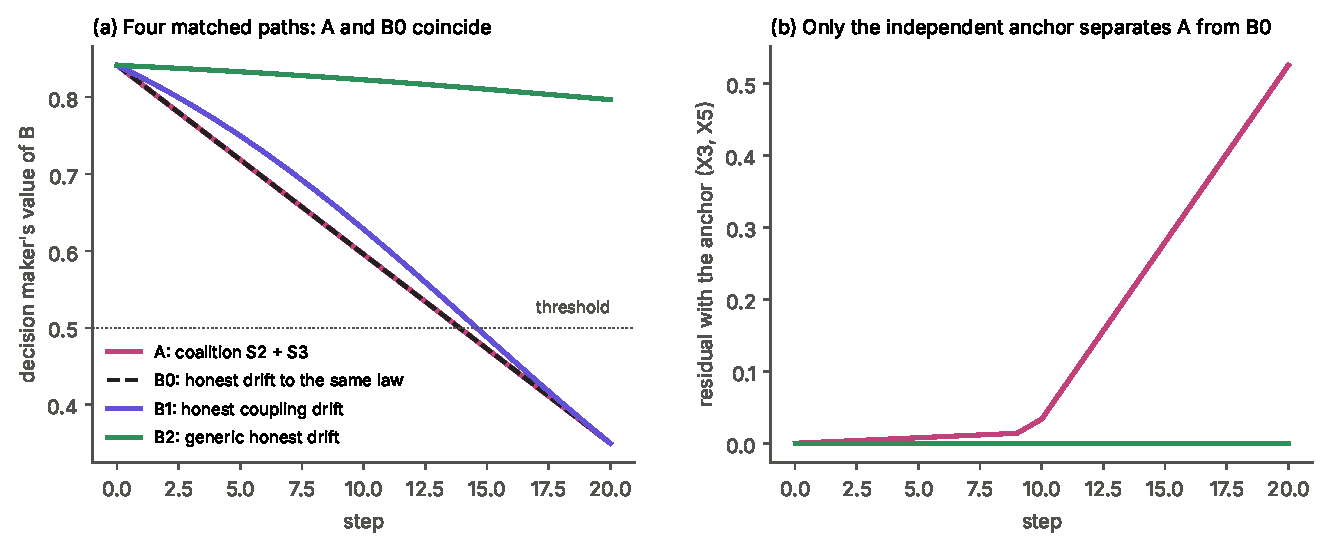
\includegraphics[width=\linewidth]{fig_miscal.pdf}
\caption{Coherent miscalibration on the bridge example. (a) The decision maker's estimate of $B$ along four paths of $20$ steps from the same start. A: the coalition $\{S_2,S_3\}$ moves its reports together towards $B=0.35$. B0: the world itself drifts to the coalition's final law, and its reports coincide with those of A. B1: an honest change in one coupling brings $B$ to the same value. B2: an honest drift of the same total size in another direction. Every path is consistent at every step. (b) The residual of the reports together with the independent anchor $(X_3,X_5)$; only path A disagrees with it.}\label{fig:miscal}
\end{figure}

\paragraph{The example.} In the bridge example, the pair $\{S_2,S_3\}$ can bring $B$ to any value in $[0,1]$, whereas $S_3$ alone could reach only $[0.365,1]$, and $S_2$ alone nothing at all. The inspection of $(X_2,X_4)$, which settled $B$ against $S_3$ acting alone, gives no protection against the pair: with it as an anchor the range is still $[0,1]$. The inspection of $(X_3,X_5)$ gives $[0.613,0.930]$, entirely above the threshold, and so protects $B$ against the pair. Which anchor helps depends on which coalition one is worried about.

\Cref{fig:miscal} compares four paths that start at the same point and last the same number of steps. Along path A only $S_2$ and $S_3$ change their reports, and $B$ moves from $0.841$ to $0.35$. Its cumulative movement towards the threshold is $D_T=0.491$, its largest single change in one report is $0.049$, and its total displacement is $1.01$. In path B0 the world itself drifts to the law at the end of path A, and the reports are \emph{exactly the same at every step}. Every statistic computed from the reports is therefore the same for both paths, whether it concerns direction, speed, which reports changed, or the residual, and no test based on the reports alone can tell them apart. The independent anchor can: along path A its disagreement with the reports grows from $0$ to $0.525$, while along B0 it stays at $0$. Path B1, an honest change in one coupling, reaches the same value of $B$ with the same $D_T$, but it changes all five reports and travels $1.54$. Path B2, an honest drift of the same total size $1.01$ in another direction, barely moves the decision ($D_T=0.045$, with $B$ ending at $0.797$). So the direction of drift separates A from B2 but not from B0 or B1; the pattern of changed reports separates A from B1 but not from B0; and only the anchor separates A from B0. Without anchors, coordinated miscalibration can look exactly like honest change.

The feedback version behaves as part~(C) predicts. A coalition that keeps moving only while the decision maker still accepts stops at the first step at which his decision flips, here after $14$ steps, with $B$ estimated at $0.497$. Every state along the way is consistent, and the coalition stays within its range.

The lesson for the decision maker is that checking his inputs against one another does not protect him against coordinated, consistent manipulation. What protects him is anchors that he controls, chosen with the coalitions he fears in mind; an inspection that settles a decision against one source may be useless against two. The direction and speed of drift are still worth studying, but only as hypotheses tested against a stated model of honest change, in a study fixed in advance; the example shows that against an honest drift ending at the same law, they cannot work at all.

\paragraph{Study 22: lineages, braids and surviving an audit.} Braids might be more at home in a different setting, where they record how information is passed from one source to another, so that a crossing is a real event: one source adopting another's view. Study 22, pre-registered, frozen and run once (\texttt{synthetic\_sections/RESULTS\_study22.md}), asked whether such braids predict whether a wrong decision survives an independent audit, using copying patterns never seen during training. The truth was hidden, one source held a false law, and the others either measured the truth or copied a neighbour; the decision concerned a context that no source reported. The braid had to improve on a strong baseline: the record of events, the graph of who copied from whom, and the decision maker's own estimate of how exposed his decision was to an audit. The study's validity check failed. On the unseen copying pattern, the baseline predicted survival no better than a constant (change in log-loss $-0.049$, $[-0.099,0.002]$), which left the main comparison with the braid uninformative. The braid did not help either ($-0.017$, $[-0.053,0.015]$), and it did not predict how many audits were needed to correct the decision ($+0.011$, $[-0.054,0.083]$). About $80\%$ of wrong decisions survived the first audit in every copying pattern, and an analysis made afterwards found nothing that predicted survival even within a single pattern. In this setting, whether a consistent but false decision survives one audit depends on the hidden truth and on which audit is drawn, as \cref{prop:miscal} suggests, and on nothing the decision maker can compute in advance. A further study would first have to make survival depend on something he can observe.


\subsection{Watching for coordinated deformation}\label{sec:watch}
Studies 21 and 22 asked the braid to find manipulation on its own, and it could not. One plausible reason is that it was fed too little: strands built from a handful of readings of the decision change order late and coarsely. This subsection does the opposite. It keeps every signal the decision maker can compute side by side, because we do not know in advance which will matter, and asks which of them warns, how early, and at what cost in false alarms.

\paragraph{What the decision maker watches.} The signals fall into groups, each attached to a different part of his information. The \emph{data} are the reported tables themselves: disagreement between reports of the same context, and disagreement between reports on the variables they share. The \emph{compatibility} group asks whether the reports have a common joint law at all: whether their supports allow any joint assignment, how far they violate the cycle inequality of the five-cycle, the residual, the number of minimal conflicts, the size of the smallest explanation, and the reach of a Farkas certificate. The \emph{hidden geometry} describes the fibre of laws the reports allow: its width along the $21$ hidden Walsh directions, which cells it forces to zero, how close it comes to the faces of the simplex, and how far each hidden move can travel. The \emph{decision} group holds the robust range, the naive estimate, the extra reach of pairs of sources, and whether conflicts fall on the sources that matter most to the decision. Then come the \emph{history} of revisions, the \emph{anchors} (inspections he controls), the \emph{observability} of each hidden direction to those inspections, the \emph{path} of the reports over time (speed, acceleration, turning, the ratio of decision movement to report movement, how many sources move at once), and finally the braid of the readings ``trust everyone except one source'', with crossing times and bursts.

\paragraph{Disagreement opens an investigation.} No single disagreement proves a lie, and none is excused just because the world might be contextual. A difference between reports of the same context is graded: exact agreement needs nothing; a difference within the stated measurement tolerance is monitored; a difference beyond it is flagged and an investigation opens. A report that an independent anchor contradicts is set aside as inconsistent with reality, without yet blaming its source. Attributing deliberate deception requires evidence from outside the model and is never done automatically. Each disagreement is also typed by where it lives. Disagreement within one context is direct evidence that some report is wrong. Disagreement that appears only around a cycle of contexts may be genuine contextuality and goes to the compatibility analysis. Disagreement across time goes to the history and the provenance of the reports.

\begin{proposition}[what reports can and cannot reveal]\label{prop:watch}
Fix the reporting contexts, a decision value $g$ linear in the law, and a threshold $\tau$.
\begin{enumerate}
\item[(a)] Two histories whose reports agree at every step give the same value of every signal computed from the reports, at every step.
\item[(b)] If the reports remain the exact marginals of the true law while the law moves inside their fibre, then $g$ of the true law stays inside the range the reports allow. Hidden movement of this kind can mislead a rule that selects one point of the fibre, but not the robust range.
\item[(c)] Let a coalition's movement change the law by $\Delta p$, while the honest world stays put; in the matched honest history the world itself makes the same move. An inspection with marginal map $M_q$ can tell the two histories apart only if $M_q\Delta p\neq0$. It does tell them apart at a step where the true table $M_qp$ lies outside the range of $M_q$ over the laws the reports allow.
\item[(d)] Suppose the coalition's reports determine $g$ given the honest ones, and that it moves its reports by at most $\delta$ per step in total $\ell^1$ distance. Let $D$ be the least such distance from the current reports to a coherent configuration with $g$ on the other side of $\tau$, which is a linear program. Then the coalition needs at least $\lceil D/\delta\rceil$ steps to cross the threshold, and the straight path achieves this.
\item[(e)] If a coalition changes the table of some context by more than the measurement tolerance, but some reporter of that context is outside the coalition, or the members change it at different times, a disagreement within that context is flagged at the first such change. Avoiding these flags requires controlling every reporter of each context it changes and moving them identically.
\end{enumerate}
\end{proposition}

\begin{proof}
(a) The signals are functions of the reports. (b) The true law belongs to the fibre at every step, so its value of $g$ lies in the range over the fibre, and the robust range contains that range. (c) In the matched history the inspection reads $M_q(p+\Delta p)$, in the other $M_qp$; if $M_q\Delta p=0$ these agree and the two histories coincide for the decision maker. If the true table leaves the range allowed by the reports, the reports together with the inspection have no common law. (d) Every step moves the reports by at most $\delta$, and the coalition must travel at least $D$. The coherent configurations form a convex set (\cref{prop:miscal}(A)) and the configurations on the far side of $\tau$ form a half-space within it, so the segment to the nearest one is coherent throughout. (e) Two reports of the same context that differ by more than the tolerance are flagged by definition.
\end{proof}

Part~(e) is simple, but it says something useful. Coordinated manipulation escapes the most reliable signal only if it is complete and perfectly synchronised over every context it touches. Giving each decision-critical context several independent reporters makes that expensive and fragile.

\paragraph{The toy.} We ran eight histories on the bridge, now with three reporters of the decision's context ($S_3$, $R_1$, $R_2$), for $20$ steps, with an independent inspection of $(X_3,X_5)$ at step $15$. The honest histories were a slow drift of the world that eventually crosses the threshold, the same change happening at once (a shock), a contextual world with no joint law but stable reports, and a world drifting along exactly the reports of the efficient coalition below. The manipulated histories were a single lying reporter; a framing attack, in which $R_2$ lies and four planted reports, two of them on the decision's own context, leave the honest $S_3$ and $R_1$ as a minority; an efficient coalition of $S_2$, $S_3$, $R_1$ and $R_2$ moving in lockstep along the straight path to the least-change false law ($B=0.35$, reached at step $10$); and a stealthy coalition moving the same reporters to the most typical false law, reached at step $20$. A signal counts as firing when it goes beyond anything it showed in the slow drift and the shock; the contextual world was not used for calibration, so a signal that fires there is a false alarm caused by contextuality.

\begin{center}\small
\begin{tabular}{lcccccc}
\toprule
 & liar & framing & efficient & stealthy & contextual & matched drift\\\midrule
disagreement within a context & 5 & 5 & -- & -- & -- & --\\
residual, conflicts, certificate & 5 & 5 & -- & -- & 0 & --\\
hidden geometry (width, faces, capacity) & -- & -- & 5 & -- & -- & 5\\
path efficiency & -- & 6 & 1 & -- & -- & 1\\
conflicts on high-leverage sources & -- & 7 & -- & -- & -- & --\\
braid crossings & 5 & 5 & -- & -- & -- & --\\
independent inspection & -- & 15 & 15 & 15 & -- & --\\\midrule
naive decision wrong from & -- & 7 & 7 & 14 & -- & --\\
\bottomrule
\end{tabular}
\end{center}

The table gives the step at which each family first fires. Speed, acceleration, turning and the number of sources moving at once never fired: the honest shock is fast and the honest drift is curved, so neither marks an attack in this world. In the framing history the naive, majority, reputation and simplest-explanation rules were wrong at $70\%$ of the steps; the robust rule was never wrong and said ``investigate''. The efficient coalition controls four reports, beyond the robust rule's assumed two, and the rule was wrong at $40\%$ of the steps, as its guarantee allows.

\paragraph{What the toy shows.}
Five findings stand out.
\begin{itemize}
\item \emph{Disagreement within a context is the cleanest signal.} It caught both attacks that involved a redundant reporter two steps before the decision went wrong, and never fired in the contextual world. Disagreement visible only around a cycle (residual, conflicts, certificates) fired from the start in the contextual world, which confirms that it needs the investigation ladder before anything is concluded.
\item \emph{Hidden geometry and path efficiency warn early but cannot attribute.} Against the efficient coalition they fired two and six steps before the flip. They fired identically on the honest world drifting along the same reports, as part~(a) requires. They mark an unusually consequential trajectory, not a culprit.
\item \emph{A stealthy coalition evades every signal computed from the reports.} Only the inspection caught it, one step after the decision had gone wrong. When to inspect matters as much as what to inspect, and part~(d) gives the clock. A coalition needs at least $\lceil D/\delta\rceil$ steps to flip a decision; in the example $D=0.683$ for $\{S_2,S_3\}$. Inspections should be scheduled within that time, not on a fixed calendar.
\item \emph{Imperfect coordination is caught at once.} When one reporter of the decision's context was not recruited, or one member followed three steps late, the disagreement within that context fired at the first step, six steps before the flip, as part~(e) predicts. The naive and majority rules still went wrong, so the flag protects the decision only if the investigation it opens is acted on.
\item \emph{The braid adds no lead time here.} Its crossings came at the same step as the disagreement within a context, which they reflect. It is a useful picture of the event, not yet an independent detector.
\end{itemize}

These are findings from one small world, chosen by hand. Study~23, described in \texttt{synthetic\_sections/PREREG\_study23\_DRAFT.md}, is drafted to test them at scale with separate calibration and evaluation seeds, honest contextual worlds in the calibration, the matched-drift control, inspection schedules driven by part~(d), varying noise, varying coalition coverage and lag, and the removal of each signal family in turn to see what it adds. It has not been frozen or run.

\subsection{The mathematical chain}\label{sec:chain}
The last four subsections build one argument, and it helps to see it in one place before turning to braids and knots. It has five links.
\begin{enumerate}
\item \emph{Reports to fibres.} Each set of reports the decision maker chooses to trust leaves a fibre of joint laws, and trusting more can only shrink it (\cref{sec:contam}). His belief is the whole assignment, not one law.
\item \emph{Fibres to conflicts and explanations.} Reports that cannot all be true form minimal conflicts, and the ways to repair them are the explanations (\cref{prop:contam}). The corrupted reports are always an explanation, though not necessarily a smallest one.
\item \emph{Explanations to reach.} A coalition can move a decision value anywhere in the range of its honest fibre, and its reach contains each member's (\cref{prop:tamper,prop:miscal}).
\item \emph{Reach to observability.} Reports alone cannot separate a coalition from an honest world that moves the same way, and an inspection separates them only if it sees the coalition's movement (\cref{prop:watch}(a), (c)).
\item \emph{Observability to protection.} An inspection protects a decision if it separates the coalition's possible endpoints from the truth, and if its result arrives before the coalition can get there (below).
\end{enumerate}

To state the last link, fix the honest reports $h$, anchors $a$ that the coalition cannot change, the true law $p^\ast$, which does not move, a decision value $g$ linear in the law, and a threshold $\tau$ with $g(p^\ast)>\tau$. For an inspection of a context with marginal map $M_q$, call
\[
\rho_q=\min\big\{\|M_q p-M_q p^\ast\|_1:\ p\ \text{matches}\ h\ \text{and}\ a,\ g(p)\le\tau\big\}
\]
its \emph{separation margin}. It is a linear program. It is positive exactly when every law that matches the honest reports, the anchors and the true inspected table has $g>\tau$, that is, when adding the inspection to the anchors excludes $\tau$ from the range of \cref{prop:miscal}(C). It is the smallest movement of the inspected table that any coalition endpoint on the far side of $\tau$ must show.

\begin{theorem}[protection against a coalition]\label{thm:protect}
Let a coalition $C$ start from honest reports at step $0$ and move its reports by at most $\delta$ per step in total $\ell^1$ distance, keeping them coherent with $h$ and $a$, and suppose its reports determine $g$ given $h$ and $a$. Let $D_C$ be the minimal flipping distance of \cref{prop:watch}(d), computed with the anchors $a$.
\begin{enumerate}
\item[(i)] If the range of $g$ over the laws matching $h$ and $a$ excludes $\tau$, the coalition can never move the decision across $\tau$ while staying coherent.
\item[(ii)] Otherwise, let $q$ be an inspection with $\rho_q>0$, ordered at step $t_0$ and returning its result $r$ steps later. If $t_0+r<\lceil D_C/\delta\rceil$, then at no step can the coalition put the decision on the far side of $\tau$ without its reports becoming incoherent with the anchors and the inspection.
\item[(iii)] (Noise.) Suppose the inspection is read with an $\ell^1$ error of at most $\eta$, the reports are otherwise exact, and the decision maker flags whenever the anchor distance $\Delta_q=\min\{\|M_qp-q_{\rm obs}\|_1:\ p\ \text{matches the current reports and}\ a\}$ exceeds a level $\kappa$. If $\rho_q>2\eta$ and $\eta\le\kappa<\rho_q-\eta$, honest reports are never flagged and every coherent coalition configuration on the far side of $\tau$ is flagged.
\end{enumerate}
\end{theorem}

\begin{proof}
(i) is \cref{prop:miscal}(C). (ii) Before the result arrives, the coalition has made fewer than $\lceil D_C/\delta\rceil$ steps and so cannot yet have reached any configuration on the far side (\cref{prop:watch}(d)). After it arrives, the inspected table $M_qp^\ast$ is an anchor too, and by the definition of $\rho_q>0$ no law matching $h$, $a$ and $M_qp^\ast$ has $g\le\tau$. Since the coalition's reports determine $g$, a far-side configuration would need such a law, so it cannot be coherent with the inspection. (iii) Honest reports are matched by $p^\ast$, so $\Delta_q\le\|M_qp^\ast-q_{\rm obs}\|_1\le\eta\le\kappa$. For a coherent far-side configuration every law that matches it and $a$ has $g\le\tau$, so $\|M_qp-M_qp^\ast\|_1\ge\rho_q$, and by the triangle inequality $\Delta_q\ge\rho_q-\eta>\kappa$.
\end{proof}

The theorem turns the two halves of \cref{sec:watch} into one rule. \emph{What} to inspect is decided by the margin $\rho_q$, which depends on the coalition one fears; \emph{when} to inspect is decided by the clock $\lceil D_C/\delta\rceil$. Part~(iii) says how much noise the inspection can tolerate: less than half its margin. On the bridge, against the pair $\{S_2,S_3\}$ with $S_1,S_4,S_5$ honest, the inspection of $(X_3,X_5)$ has $\rho_q=0.225$ and leaves the range $[0.613,0.930]$, so it protects $B$ if it is read with error below $0.1125$; the inspection of $(X_2,X_4)$ has $\rho_q=0$ and protects nothing. With $D_C=0.683$ and $\delta=D_C/7$, its result must arrive within $6$ steps of the start. Random far-side configurations of the pair, read against an inspection with error $0.101$, all had anchor distance at least $0.148$, above the flag level $0.1125$, while the honest reports never exceeded $0.101$. BK9 and BK10 check these numbers. The theorem assumes the honest reports are exact; with noisy reports the fibres must be replaced by tolerance fibres, which we have not done.

\subsection{What braids and knots carry}\label{sec:braidknot}
Braids and knots have appeared in several roles in this note: as crossing logs of decision streams (\cref{sec:ledgerdm}), as pseudo-diagrams whose crossings are uncertain (\cref{prop:pseudoknot,prop:figeight}), and as pictures of manipulation that Studies~19--22 and \cref{sec:watch} found to add nothing. This subsection says exactly what information they can carry, and checks the one construction that seemed to support them.

\begin{proposition}[the content of braids and knots built from data]\label{prop:braidcontent}
Let $H$ be a history of reports and let every strand be computed from $H$.
\begin{enumerate}
\item[(1)] \emph{Scalar strands.} If each strand is one number per step, its braid word is determined by the sequence of order exchanges together with the values of the over/under rule at those exchanges. It carries nothing else.
\item[(2)] \emph{Planar strands.} If each strand is a point in the plane and no two collide, the history is a path in the configuration space $\mathrm{Conf}_k(\mathbb C)$, and its braid is the homotopy class of that path with fixed ends. It does not change under reparametrisation of time or under perturbations that keep the strands apart. For a pure braid, the part detected by commuting quantities is the vector of pairwise winding numbers, since these generate the abelianisation of the pure braid group; what lies beyond them, such as commutators, is detected by Milnor's invariants of the closure.
\item[(3)] \emph{Knots and links.} A knot or link needs the history to be closed, either because it returns to where it began or by a declared closure. Closed curves embedded in $\mathbb R^n$ with $n\ge4$ are all unknotted, so a knot type belongs to a chosen three-dimensional shadow of the data, not to the data themselves.
\item[(4)] \emph{Uncertain diagrams.} If the crossings of a diagram are random signs with joint law $q$, the expectation of any invariant $f$ of the resolved diagram is the linear functional $\mathbb E_qf=\sum_S\hat f(S)\,\mathbb E_q\big[\prod_{i\in S}e_i\big]$. It is determined by the observed tables exactly when its Walsh support is covered by them, and otherwise it ranges over an interval, with tamper budgets as in \cref{prop:tamper}.
\item[(5)] \emph{The ceiling.} A braid or knot computed from $H$ carries no information about anything beyond what $H$ carries: for any target $Y$, $I(Y;\beta\mid H)=0$. It can add information only relative to a summary $X$ of $H$, through $I(Y;\beta\mid X)$.
\end{enumerate}
\end{proposition}

\begin{proof}
(1) The braid word is built from the exchanges and the rule, by construction. (2) A braid is by definition a homotopy class of paths in configuration space, and a homotopy that keeps the strands apart, including a change of time parametrisation, does not change it. The abelianisation of the pure braid group is free abelian on the generators $A_{ij}$, and the induced map sends a pure braid to its pairwise winding numbers \cite{Artin1947,Birman1974}. Milnor's invariants of closures of pure braids detect commutators, and for the closures of pure braids they classify links up to link homotopy \cite{Milnor1954,HabeggerLin1990}. (3) The unknotting is classical \cite{Rolfsen1976}. (4) This is linearity of expectation and the Walsh criterion of \cref{prop:pseudoknot}. (5) $\beta$ is a function of $H$.
\end{proof}

Parts (1) and (2) explain the earlier null results. The strands of Studies~19--22 were scalar, so their braids were the order-exchange sequence and nothing more, and every scenario drifted in one direction, so there was nothing to wind. The next two examples show what genuinely topological content looks like.

\paragraph{A braid that pairwise statistics cannot see.} Take three strands in the plane, and let $A=\sigma_1^2$ and $B=\sigma_2^2$ be full twists of strands $1,2$ and of strands $2,3$, realised by turning the pair once about its midpoint. Compare four orderings of the same four moves (\cref{fig:commutator}). In each, every pairwise winding number is zero, the path length is the same ($25.13$) and the strands stay at least $0.9$ apart. Using Artin's faithful action on the free group and the Magnus expansion of the longitudes, the four closures have:
\begin{center}\small
\begin{tabular}{lcccc}
\toprule
ordering & $ABA^{-1}B^{-1}$ & $BAB^{-1}A^{-1}$ & $AA^{-1}BB^{-1}$ & $ABB^{-1}A^{-1}$\\\midrule
pairwise linking numbers & $0,0,0$ & $0,0,0$ & $0,0,0$ & $0,0,0$\\
second-order coefficient (triple invariant) & $+1$ & $-1$ & $0$ & $0$\\
the braid & non-trivial & non-trivial & trivial & trivial\\
signed area of $(\theta_{12},\theta_{23})$, over $(2\pi)^2$ & $+1.000$ & $-1.000$ & $0.000$ & $0.000$\\
\bottomrule
\end{tabular}
\end{center}
The commutator's closure has the same Jones and Alexander polynomials as the Borromean rings, and the same triple invariant as the Borromean braid $(\sigma_1\sigma_2^{-1})^3$. (Sign conventions for Milnor's invariants differ between authors; we use the coefficient of $X_1X_2$ in the longitude of strand $3$.) So the commutator carries information that no pairwise statistic and no coarse summary carries: the order in which cancelling rotations happen.

The last row shows what that information is in ordinary terms. Let $\theta_{12}$ and $\theta_{23}$ be the unwrapped angles between strands $1,2$ and $2,3$. In this realisation the signed area enclosed by the curve $(\theta_{12},\theta_{23})$, divided by $(2\pi)^2$, equals the triple invariant to three decimals, and jitter of size $0.03$ that keeps the strands apart changes it by less than $0.002$. That area is the antisymmetric second-order term of the path signature, an iterated integral in the sense of Chen \cite{Chen1977}. In general Milnor's invariants of pure braid closures are iterated integrals of the winding forms \cite{Kohno1985}; we claim the simple area identity only for the realisation above. The practical meaning is twofold. A detector that computes second-order path signatures of the right angles already has this information, so a fair test of braids must include that baseline, not only coarse summaries. And the information exists only if features actually turn around one another, which nothing in our threat models forces a coalition to do.

\begin{figure}[!htbp]\centering
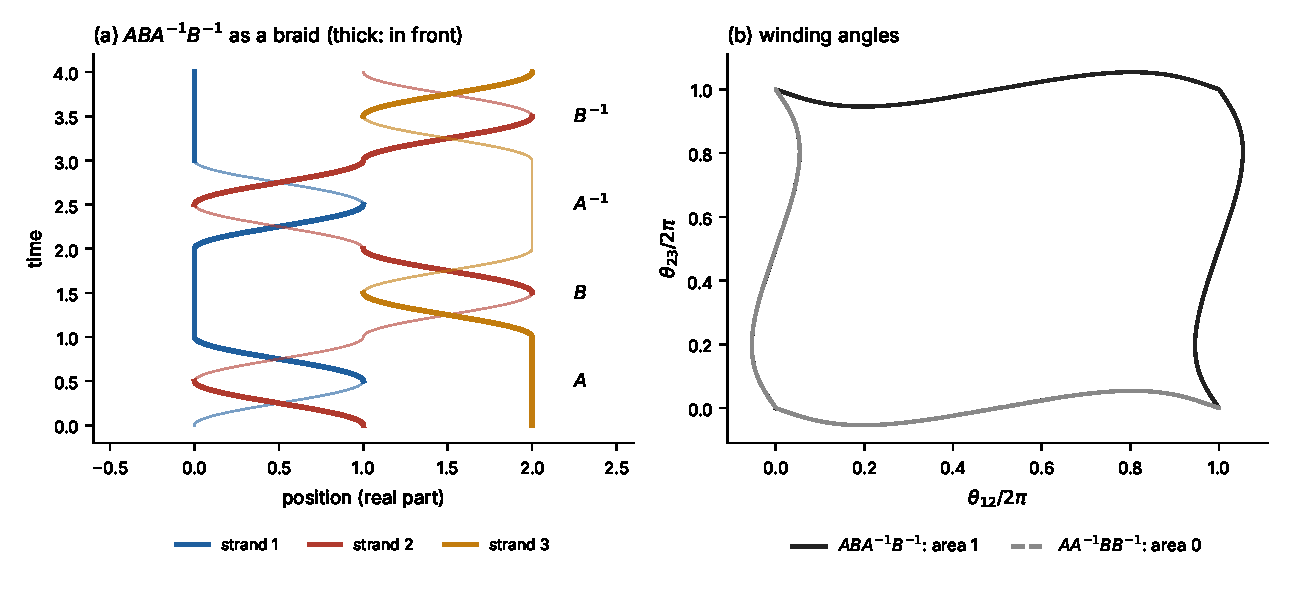
\includegraphics[width=0.92\linewidth]{fig_commutator.pdf}
\caption{The commutator braid. (a) $ABA^{-1}B^{-1}$ drawn over time, with $A=\sigma_1^2$ and $B=\sigma_2^2$ realised as full turns; the thick parts are in front. (b) The winding angles $(\theta_{12},\theta_{23})$. The commutator encloses area $(2\pi)^2$; the ordering $AA^{-1}BB^{-1}$, with the same moves and the same pairwise windings, encloses none.}\label{fig:commutator}
\end{figure}

\paragraph{A knot invariant as a target, not a detector.} Part~(4) has a sharp form. On $\{+1,-1\}^4$ take the two laws $q_\pm(e)=\tfrac1{16}(1\pm\theta e_1e_2e_3e_4)$ with $0<\theta\le1$. They agree on every moment of order at most three, so any data on at most three crossings at a time are the same under both. For any invariant $f$ of the resolutions, $\mathbb E_{q_+}f-\mathbb E_{q_-}f=2\theta\hat f(\{1,2,3,4\})$. On the figure-eight pseudo-diagram of \cref{prop:figeight}, knottedness is $\tfrac14(1+e_1e_2)(1+e_3e_4)$, so its top coefficient is $\tfrac14$ and $P_{q_+}(\text{knotted})-P_{q_-}(\text{knotted})=\theta/2$. The Jones polynomial also has a non-zero top coefficient. The writhe $e_1+e_2+e_3+e_4$ has degree $1$ and the same expectation under both laws, so not every invariant reaches degree four, and the degree must be computed for each invariant and diagram. The decision maker cannot compute $\mathbb E_qf$ from data that look at three crossings at a time; under both laws he sees the same thing. What the invariant gives him is a reason why a decision may depend on a hidden direction: knottedness here is a conjunction of two pairwise events, and conjunctions have top-order terms. The range it can take, and the budget a coalition has over it, are computed by the linear programs we already have. If the two twist regions happen to be independent, the fourth moment is the product of the pair moments and becomes identified. BK4 checks these identities.

\paragraph{The sources as a bundle.} A different picture was proposed during this work. Think of the sources as strands of a bundle: honest data keep the bundle tight, and poisoning makes strands separate, cross and tangle, with the tangle growing as simple explanations stop working. We tested this directly on the histories of \cref{sec:watch} and two more, a coalition that pumps a false law and then retreats, and a \emph{cascade} in which a liar is followed by planted reports and then by the recruitment of an honest source. For each persistent source $x$ and step $t$, let $s_x(t)$ be the residual of everything except $x$ (low when removing $x$ explains the most) and $v_x(t)$ the decision value without $x$. The strand of $x$ is the point $z_x(t)=s_x(t)+\mathrm i\,v_x(t)+\varepsilon\,\omega_x$, where the $\omega_x$ are seven fixed points on the unit circle, moved linearly between steps. The small ring $\varepsilon\omega_x$ is needed because consistent snapshots would otherwise put several strands at the same point. The braid is read by projecting onto the suspicion axis $s$, with over and under decided by the other coordinate.

\begin{proposition}[coherent histories give trivial bundle braids]\label{prop:cohtrivial}
If every snapshot of a history is coherent, its bundle braid is trivial for every ring size $\varepsilon>0$ and every projection direction.
\end{proposition}

\begin{proof}
If all reports are coherent, so is every subset, and so $s_x(t)=0$ for every $x$ and $t$. Each strand then moves on the vertical line through $\varepsilon\,\mathrm{Re}\,\omega_x$, and these lines are distinct because no two of the seven ring angles $2\pi k/7+0.3$ have the same cosine. Sliding every strand along its own line to its starting height is a homotopy through configurations without collisions, so the braid is trivial.
\end{proof}

So a lockstep coalition, which keeps every snapshot coherent, leaves the bundle untwisted until an inspection contradicts it. This is \cref{prop:watch}(a) seen through the braid: the bundle can register a loss of coherence, and a coalition's whole skill is not losing it.

The incoherent histories raise a different problem, and it decides what the braid can carry. Over thirty drawing conventions (ring sizes from $0.005$ to $0.08$, projection angles from $-0.02$ to $0.05$ radians), the single liar gave five different braid elements, and the framing and cascade histories four each, with closures of between two and five components. A noise of $0.003$ in the reports changed the cascade braid again. The reason is that the data tie the strands. In $16$ to $18$ of the $21$ steps several sources have exactly the same suspicion height: once the liar speaks, removing any one of the six honest sources leaves the same conflict, so all six sit at $0.983$. The data cannot order them, and whether and how their strands cross is decided by the drawing convention. In short, \emph{a crossing carries information only between strands that the data separate}. The knot of the cascade closure that an earlier version of this toy reported, with determinant~$3$, came from its tie-breaking rule and does not survive this test. BK6 records the failure. \Cref{sec:tiebridge} revisits it with the ring sent to zero and the history closed, and finds that part of the instability came from how the open braids were compared; the ties themselves remain.

What does survive every convention, and the noise, is the sequence of \emph{suspect sets}: the sources whose removal leaves a residual within $0.01$ of the lowest. \Cref{fig:bundle} shows it with the smallest explanation, and the table summarises all ten histories.
\begin{center}\footnotesize
\begin{tabular}{@{}lllcl@{}}
\toprule
history & smallest explanation & suspect sets & bundle braid & co-revising group\\\midrule
honest drift & $0$ & none & trivial & all seven\\
honest shock & $0$ & none & trivial & none\\
matched honest drift & $0$ & none & trivial & $S_2,S_3,R_1,R_2$\\
honest contextual world & $1$ throughout & $\{S_1,S_2,S_4,S_5\}$ & trivial & none\\
pump and retreat & $0$ & none & trivial & $S_2,S_3,R_1,R_2$\\
single liar & $0\to1$ & none $\to\{R_2\}$ & not determined & none\\
framing & $0\to2\to$ none & none $\to\{R_2\}\to\{S_3,R_1\}$ & not determined & none\\
cascade & $0\to1\to3\to$ none & none $\to\{R_2\}\to\{S_3,R_1\}$ & not determined & none\\
lockstep (efficient) & $0\to$ none at step $15$ & none $\to\{S_4\}$ & trivial & $S_2,S_3,R_1,R_2$\\
lockstep (stealthy) & $0\to$ none at step $15$ & none $\to\{S_4\}$ & trivial & $S_2,S_3,R_1,R_2$\\
\bottomrule
\end{tabular}
\end{center}
Here ``none'' in the explanation column means that no set of at most three reports explains the conflict. The naive decision was wrong at $6$ steps of the pump-and-retreat history, $14$ of framing, $13$ of the cascade, and $14$ and $7$ of the two lockstep histories, and never in the others. The last column is explained below.

\begin{figure}[!htbp]\centering
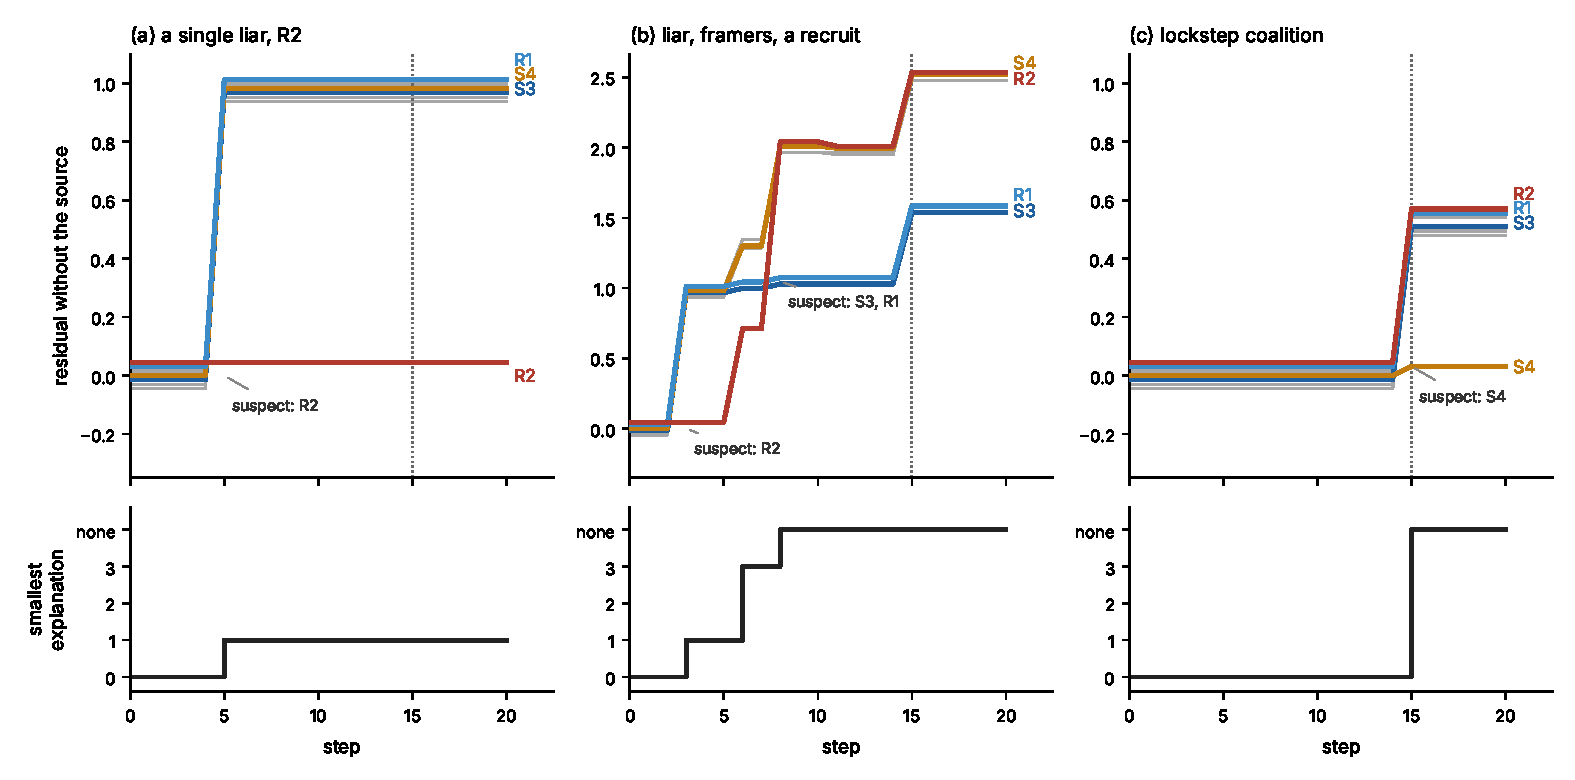
\includegraphics[width=\linewidth]{fig_bundle.pdf}
\caption{The sources as a bundle. Top: the residual of all reports except one source, for each source (honest strands in grey, offset slightly so that tied strands stay visible), with the inspection at step $15$ dotted. Bottom: the smallest set of reports whose removal leaves the rest consistent (``none'': no set of at most three). (a) A single liar drops out of the bundle and is the suspect throughout. (b) In the cascade, the planted reports make the honest reporters $S_3$ and $R_1$ the suspects, while the smallest explanation grows from one report to more than three. (c) A lockstep coalition leaves the bundle tight until the inspection, after which the honest $S_4$ is the suspect.}\label{fig:bundle}
\end{figure}

Three things stand out. First, honest contextuality and deception look different even though both produce conflicts: the contextual world shows a stable split from the first step, blamed on the four sources of the cycle that have no second reporter, while deception shows a split that changes. Second, the single liar and the cascade, both deceptive, differ in exactly the way the bundle picture suggested, but the difference is carried by the suspect sets and the explanation sizes, not by a braid. In the cascade the blame passes from the liar $R_2$ to the honest pair $\{S_3,R_1\}$ at the step where the smallest explanation jumps from three reports to more than three, and the naive decision goes wrong at the same time. Third, the lockstep coalition, once the inspection contradicts it, is blamed on the honest $S_4$, because the coalition is larger than any explanation the decision maker considers. In both of the last two cases attribution has become unreliable, and a change of suspect set at the moment the explanations grow is the warning. This supports the rule of \cref{sec:watch}: disagreement opens an investigation, and attribution is never automatic. BK5, BK7 and BK8 check these statements.

\paragraph{Who moved together.} The suspect sets fail exactly where the coalition is coherent: they name nobody while it moves, and the honest $S_4$ once the inspection contradicts it. A different signal, from the literature on coordinated online campaigns, fills this gap. Iannucci, Muratore, Matakos and Kivel\"a \cite{Iannucci2025} detect coordinating accounts not by anything each does alone but by repeated co-action: two accounts are linked each time they take the same kind of action, with a weight that decays with the delay between them and is divided by the number of accounts acting at that moment, and groups are then found in the resulting network. In our setting a source acts when it revises its report. Built this way (decay rate $1$ per step, link threshold $0.5$), the co-revision network picks out exactly $\{S_2,S_3,R_1,R_2\}$ in the efficient, stealthy and pump-and-retreat histories, the three in which the suspect sets name nobody, or the honest $S_4$. It does not separate them from the matched honest drift, where the same four sources revise together because the world moves only in their contexts; that is \cref{prop:watch}(a) again, since the network is computed from the reports. In the honest drift all seven sources revise together, and a one-time shock or a single liar forms no repeated group. So co-revision says \emph{who moved together}, not who lied. Combined with an anchor it does what the explanations could not: once the inspection contradicts the reports, the group that moved together, not the smallest explanation, is the natural place to look, and here it is the right one. BK11 checks these groups.

The vocabulary of Abramsky and Car\`u \cite{AbramskyCaru2019} fits the table. They distinguish \emph{local} disagreement (two sources contradict each other on shared variables), \emph{global} disagreement with local agreement (no single global truth, though every pair agrees; for probability tables this is exactly contextuality), and \emph{complete} disagreement (combining the sources leaves nothing; strong contextuality in the possibilistic case). The single liar, framing and the cascade produce local disagreement within the decision's context. The honest contextual world produces global disagreement with local agreement. The lockstep coalitions produce no disagreement of any kind until the inspection, so no theory of disagreement between sources can see them, and co-movement or anchors are needed. Abramsky and Car\`u also show that for relational and logical information detecting global disagreement is an inference problem, so that the local-computation algorithms of generic inference apply to it; for probability tables the corresponding test is the linear program behind the residual, and the acyclic case, where pairwise agreement is enough, is \cref{prop:contam}(1).

\paragraph{Study 24: attribution under contamination.} Whether these patterns hold beyond ten hand-built histories was tested in a pre-registered study, frozen before its single run (\texttt{RESULTS\_study24.md} in \texttt{synthetic\_sections}). It drew $600$ random worlds on the bridge structure, with one or two extra reporters of the decision's context, ten kinds of history (single liars, framing, cascades, three kinds of lockstep coalition, and four honest kinds), sampling noise in half of them, and one inspection at a random step. The primary target was \emph{wrong attribution}: at the last step the suspect set is non-empty and contains no deceptive source. It happened in $29\%$ of the test histories, most often under framing ($69\%$) and in cascades ($75\%$), and in $32$--$41\%$ of the efficient and stealthy coalitions. The results were these.
\begin{itemize}
\item \emph{Co-revision found the coalitions that attribution by explanation missed.} Against lockstep coalitions the suspect set overlapped the true coalition by $0.05$ on average (Jaccard index), and the co-revision group by $0.83$; the paired difference was $0.78$ $[0.73,0.82]$, $n=180$. In none of the $180$ histories did the co-revision group contain an honest source. When it missed members, they were coalition members whose reports the attack never needed to move. This replicates, on fresh seeds, what the development seeds had already shown. As \cref{prop:watch}(a) requires, the honest world drifting along a coalition's reports produced a co-revision group just as often ($100\%$ against $92\%$), and honest drift and shocks gave a group of all sources or none in $142$ of $142$ cases.
\item \emph{Attribution instability was not shown to help.} Adding the record of suspect-set changes to the snapshot signals lowered the held-out log-loss for wrong attribution by $0.034$, but the interval $[-0.067,+0.002]$ crosses zero, so the pre-registered hypothesis is not supported. After the fact (and so only as a pointer), the attribution record and co-revision together lowered it by $0.058$ $[-0.109,-0.005]$.
\item \emph{Braids and knots added nothing}, as expected: $+0.006$ $[-0.007,+0.018]$ given the other families. The bundle braid was determined by the data in only $27$--$55\%$ of histories.
\item Telling a cascade from a single liar needed nothing beyond the snapshot, again as expected.
\end{itemize}
The practical reading is a division of labour. Explanations say which reports cannot all be true, and when the coalition is larger than the explanations considered they point at the wrong sources. Co-revision says which sources moved together, never named an honest source here, but cannot distinguish a coalition from an honest world that moved the same way. Anchors decide between the two (\cref{thm:protect}). None of these is a verdict; each opens an investigation.

\paragraph{Status.} \Cref{thm:protect} and \cref{prop:braidcontent,prop:cohtrivial} are proved, with parts (2) and (3) of \cref{prop:braidcontent} resting on cited results. The commutator table is exact computation, and the area identity is a computed fact about one realisation. The bundle and co-revision results are computations on hand-built histories, tested at scale by Study~24; the failure of the bundle braid is reported as a finding, not explained away. All checks are in \texttt{engine/check\_braidknot.py}.


\subsection{The bridge: ties, resolutions and probability}\label{sec:tiebridge}
Three constructions have run through this part of the note. In the first, crossings are random signs with a joint law, and we ask what incomplete data say about the knot (\cref{prop:pseudoknot,prop:figeight}). In the second, strands move in the plane and their paths are braids with windings and Milnor invariants (\cref{prop:braidcontent}). In the third, the history of the sources is drawn as strands (\cref{sec:braidknot}). The first two are mathematics; the third was exploratory, and it failed the test of being well defined. This subsection supplies the missing link. It shows when a source history gives a genuine braid, and that where it does not, it gives exactly the kind of object of the first construction, with its probability law coming from the way the data are perturbed.

\paragraph{The setting.} Let $Z(t)=(z_1(t),\dots,z_k(t))\in\mathbb C^k$ be a closed piecewise-linear history of $k$ labelled points, one per source; in the toy, $z_x=s_x+\mathrm iv_x$ as in \cref{sec:braidknot}, closed by the straight path back to the first step, with points closer than $10^{-6}$ identified (the ties in the toy are below $10^{-7}$ and the genuine separations above $3.9\times10^{-3}$). Two sources are \emph{tied} at a step if their points coincide. For a direction $\omega\in\mathbb C^k$ with distinct coordinates and a small $\varepsilon>0$, the regularised history $Z+\varepsilon\omega$ moves every source off its ties by a fixed offset; when it has no collisions it is a pure braid, and its closure is a link with one component per source. For a pair $x,y$ write $D=z_x-z_y$ and $\delta=\omega_x-\omega_y$, and define the pair's \emph{walls} in the $\delta$-plane: the ray $-\mathbb R_{>0}d_0$ for every segment on which $D$ goes from $d_0\ne0$ to $0$ (the pair merges), the ray $-\mathbb R_{>0}d_1$ for every segment on which it goes from $0$ to $d_1\ne0$ (it splits), and the line through $d_1-d_0$ for every segment on which $D$ passes through $0$ in its interior. The walls cut the $\delta$-plane into sectors, and the \emph{resolution} of $\omega$ is the list of sectors in which the differences $\omega_x-\omega_y$ fall.

\begin{proposition}[from source histories to pseudo-links]\label{prop:tiebridge}
In this setting:
\begin{enumerate}
\item[(i)] If no difference $\omega_x-\omega_y$ lies on a wall of its pair, there is $\varepsilon_0>0$ such that $Z+\varepsilon\omega$ has no collisions for $0<\varepsilon<\varepsilon_0$, and its link does not depend on $\varepsilon$ or on the direction of projection used to read it. The link is locally constant in $\omega$ off the walls.
\item[(ii)] The linking number of sources $x$ and $y$ depends only on the sector of $\omega_x-\omega_y$ among the walls of that pair.
\item[(iii)] Walls arise only at steps where a pair becomes tied or stops being tied, or passes through a tie. If no two sources are ever tied, there are no walls, and the link is the same for every $\omega$: the data determine the topology. A pair that is tied at every step has no walls and linking number $0$; so if all sources are tied at every step, as in a coherent history, the link is trivial, which contains \cref{prop:cohtrivial}. A pair with a single wall direction has one sector, and its linking number is again determined by the data.
\item[(iv)] If $\omega$ is random with law $\mu$, the resolution is random with the image law $q$, and the expectation of any link invariant $f$ is $\mathbb E_\mu f=\sum_rq(r)f(r)$. If $\omega$ is an isotropic Gaussian, each pair's sector has probability equal to its angle divided by $2\pi$, so the expected linking number of each pair is computed from that pair's walls alone. Invariants that depend on several pairs' sectors at once need their joint law, and are subject to the Walsh criterion of \cref{prop:pseudoknot}.
\end{enumerate}
\end{proposition}

\begin{proof}
(i) A pair collides at a time where $D+\varepsilon\delta=0$. On a segment where $D$ stays at distance at least $c>0$ from $0$ this is impossible once $\varepsilon|\delta|<c$. Where $D$ is identically $0$ it is impossible because $\delta\ne0$. Where $D$ goes linearly from $d_0\ne0$ to $0$, the equation $(1-u)d_0+\varepsilon\delta=0$ has a solution with $u\in[0,1)$ exactly when $\delta\in-\mathbb R_{>0}d_0$, for every $\varepsilon$; splitting is the same with $d_1$. Where $D$ passes through $0$ inside the segment, a collision needs $\varepsilon\delta$ to lie on the segment $-D([0,1])$, which passes through $0$; for $\delta$ off the line through that segment's direction this fails for all small $\varepsilon$. There are finitely many segments, so a common $\varepsilon_0$ exists. Varying $\varepsilon$ in $(0,\varepsilon_0)$, or $\omega$ along a path that avoids the walls (with $\varepsilon_0$ uniform on the compact path), is an isotopy of closed braids, which does not change the link; reading the same geometric braid from another direction does not change it either. (ii) The linking number of the two components is the winding number of $D+\varepsilon\delta$ around $0$ over the closed history, which can change only when the curve passes through $0$, that is, when $\delta$ crosses a wall of the pair. (iii) The walls were defined only at such segments. A pair tied throughout has $D+\varepsilon\delta=\varepsilon\delta$, a constant, whose winding number is $0$. A single ray has a connected complement, so by (ii) the pair's linking number is the same for every admissible $\delta$. (iv) The first statement is the change of variables. For an isotropic complex Gaussian $\omega$, each $\omega_x-\omega_y$ is an isotropic complex Gaussian, whose argument is uniform. The last statement is linearity of expectation together with \cref{prop:pseudoknot}.
\end{proof}

\paragraph{The toy.} We applied the proposition to the ten histories of \cref{sec:braidknot}, regularising with $400$ random directions each.
\begin{center}\small
\begin{tabular}{@{}p{0.42\linewidth}cccc@{}}
\toprule
history & walls & resolutions & link types & entropy (bits)\\\midrule
honest drift, shock, matched drift, pump and retreat, contextual world & $0$ & $1$ & $1$ (trivial) & $0$\\
lockstep coalitions (efficient, stealthy) & $6$, $9$ & $1$ & $1$ (trivial) & $0$\\
single liar & $16$ & $3$ & $3$ & $0.24$\\
framing & $40$ & $354$ & $336$ & $8.4$\\
cascade & $38$ & $372$ & $348$ & $8.5$\\
\bottomrule
\end{tabular}
\end{center}
Every regularised link was the same for $\varepsilon\in\{10^{-4},10^{-5},10^{-6}\}$ and three directions of projection ($2250$ loops), each pair's linking number was a function of that pair's sector alone, and the sector frequencies matched their angles to within $0.016$. The \emph{entropy} is that of the resolution under isotropic directions: it measures how much of the topology the data leave open.

Four things follow, and they sharpen \cref{sec:braidknot}.
\begin{itemize}
\item \emph{The earlier failure was partly one of reading.} There we compared open braids drawn with rings of different sizes and from different directions, which changes the frame at both ends. Read as closed histories with the ring sent to zero, honest and lockstep histories have one resolution and the trivial link. The determinant~$3$ of the prototype still came from a ring that was not small, and remains withdrawn.
\item \emph{How tangled the history is becomes a number.} An honest history leaves no topology open, a single liar leaves a quarter of a bit, and framing and the cascade leave more than eight bits: hundreds of different links are compatible with the same data. This is the precise form of the intuition that deception makes the history convoluted. It is not a detector of coalitions: the lockstep coalition leaves nothing open, because it stays coherent.
\item \emph{The open topology is pairwise here.} Wherever a triple's linking numbers vanish, its triple invariant was zero in every sampled resolution ($14{,}432$ cases), so in this toy everything the data leave open is a set of pairwise linking numbers, each with its own distribution. Higher-order invariants of the kind in \cref{fig:commutator} would need strands that genuinely turn around one another.
\item \emph{Noise is not a regularisation.} Fresh sampling noise at every step (size $0.003$) left most ties in place, since they come from the structure of the conflict, and made tied strands wind around each other at random: in nine noisy histories, $4$ to $12$ pairs had linking numbers no fixed direction allows, all of them pairs tied in the clean data, while every pair the data separate kept a linking number the clean resolutions allow. A persistent bias of each source is a fixed $\omega$ and fits the proposition; independent noise at every step does not, and on tied pairs the link then records the noise.
\end{itemize}
So the bridge is this. A source history gives a genuine link exactly on the pairs of sources that the data keep apart. On pairs that the data tie, it gives a pseudo-link whose resolutions are sectors cut out by the history itself, and whose probabilities come from the model of how the data are perturbed. That is the object of the first construction, and its invariants are identified, or bounded, by the same Walsh criterion. TB1--TB8 in \texttt{engine/check\_tiebraid.py} check these statements.


\subsection{Ordered co-revision}\label{sec:ordrev}
Study~24 found that the group of sources that revise together names a coordinated coalition. It says nothing about the \emph{order} of their revisions. So we ask a question that is mathematical, not predictive: can braid or knot invariants distinguish different orders of co-revision that membership and pairwise statistics cannot, and if so, how do they compare with the ordinary record of the order? The outcome is discrimination between ordered histories, not detection of sabotage.

\paragraph{The construction.} Place the sources at positions $1,\dots,k$ on a line. An event is a co-revision of an adjacent pair $\{i,i+1\}$ with a sign: $+1$ when the two move towards each other's view (an adoption, or a reinforcement if repeated), $-1$ when they move back (a withdrawal, or a reversal after an adoption). A history is a word of events. Each event is realised geometrically as one full turn of the two strands about their midpoint, so that it is the pure braid $A_i^{\pm1}=\sigma_i^{\pm2}$; the strands keep unit spacing otherwise, and the closure is the standard one. Two events are \emph{independent} if their pairs are disjoint. The ordinary record of the order is the \emph{path signature} of the cumulative count path, which has one coordinate per pair and moves one unit per event; its level-$m$ terms are the iterated sums of order $m$ \cite{Chen1977}. Its \emph{partially commutative} version is the image of the signature in the algebra where the variables of independent pairs commute, $X_iX_j=X_jX_i$ for $|i-j|\ge2$; it keeps the iterated sums but forgets the relative order of independent events.

The braid enters through three assumptions, which we state because the topology is imposed by them, not derived from the data. \emph{(E1)} The sources are placed on a line and only neighbouring pairs co-revise. \emph{(E2)} Each event is one full twist of its pair, with its sign as the direction of the twist. \emph{(E3)} Two events are independent exactly when their pairs are disjoint. Under (E1)--(E3) the independence structure of events is a path, which the squares of the braid generators represent faithfully (below). If three sources co-revise with one another, or one source with several others not next to it on the line, the squares no longer represent the independence structure, and a different encoding would be needed.

\begin{proposition}[ordered co-revision]\label{prop:ordrev}
\begin{enumerate}
\item[(i)] Two histories give the same braid if and only if one can be turned into the other by swapping adjacent independent events and cancelling an event next to its reversal. In particular the braid depends only on the trace of the history in the sense of Cartier and Foata, up to such cancellations.
\item[(ii)] For three sources (pairs $\{1,2\}$ and $\{2,3\}$), no two events are independent, and two histories give the same braid if and only if their freely reduced words agree, which holds if and only if their count paths have the same signature.
\item[(iii)] For three sources and a history with no net co-revision on either pair, the pairwise linking numbers of the closure vanish, and Milnor's triple invariant equals the signed area enclosed by the count path, that is, the antisymmetric part of its level-2 signature.
\item[(iv)] For any number of sources, two histories give the same braid if and only if their count paths have the same partially commutative signature; the ordinary signature separates more.
\end{enumerate}
\end{proposition}

\begin{proof}
(i) Two separate facts are needed. The first is combinatorial: in the right-angled Artin group on the path (generators $a_1,\dots,a_{k-1}$, with $a_i,a_j$ commuting exactly when $|i-j|\ge2$), two words are equal exactly when they are related by swapping adjacent commuting letters and free cancellation; this is the solution of the word problem for such groups, through the trace monoid \cite{CartierFoata1969}. The second is the embedding: Collins proved that the squares $\sigma_1^2,\dots,\sigma_{k-1}^2$ satisfy no relations in the braid group other than these commutations \cite{Collins1994}, so the homomorphism $a_i\mapsto\sigma_i^2$ from the right-angled Artin group into the braid group is injective. Together they give (i). We also checked the statement directly on the enumerated families below. (ii) For three sources the group is free on $A_1,A_2$, so equality is equality of reduced words. A lattice path is determined by its signature up to backtracking \cite{HamblyLyons2010}, and backtracking in the count path is exactly cancellation of an event with its reversal. (iii) The linking numbers are the net counts. For a word in $A_1,A_2$ let $c_{12}$ be the sum of $\epsilon\epsilon'$ over pairs of events in which an $A_1^{\epsilon}$ precedes an $A_2^{\epsilon'}$, and $c_{21}$ the same with the roles exchanged. Then $c_{12}+c_{21}$ is the product of the net counts, here $0$, and the signed area of the count path is $\tfrac12(c_{12}-c_{21})=c_{12}$. In the free group on $A_1,A_2$, $c_{12}$ is the coefficient of $X_1X_2$ in the Magnus expansion, and a word with zero net counts equals $[A_1,A_2]^{c_{12}}$ modulo the third term of the lower central series. Milnor's invariant of length three is additive on the commutator subgroup and vanishes on the third term \cite{Milnor1954,HabeggerLin1990}, and $[A_1,A_2]$ has invariant $1$ (\cref{sec:braidknot}), so the invariant is $c_{12}$. (iv) The group of (i) is the free partially commutative group on the path. Its Magnus map, which sends a generator $a$ to $1+X_a$ in the algebra of power series in which the variables of independent generators commute, is injective, and its filtration gives the lower central series \cite{DuchampKrob1992}. The map $a\mapsto e^{X_a}$, which gives the partially commutative signature, differs from the Magnus map by the substitution $X\mapsto\log(1+X)$ in each variable, which is invertible and preserves the filtration, so the two determine each other level by level. The ordinary signature is a lift of the partially commutative one, so it is at least as fine, and it separates histories that differ by swapping independent events.
\end{proof}

\paragraph{Exact enumeration.} Take three sources and every ordering of two adoptions and two withdrawals on each pair: $2520$ histories with identical counts, identical co-revision membership, and identical pairwise linking numbers. The invariants cut them into these classes.
\begin{center}\small
\begin{tabular}{@{}lc@{}}
\toprule
what is compared & classes\\\midrule
counts, membership, net windings, linking numbers & $1$\\
triple invariant $=$ signed area $=$ level-2 signature & $9$\\
degree-3 Magnus coefficients of the longitudes $=$ level-3 signature & $195$\\
level-4 signature & $249$\\
braid $=$ reduced word $=$ full signature (level~5 already suffices) & $297$\\
Jones and Alexander polynomials of the closure & $10$\\
\bottomrule
\end{tabular}
\end{center}
With four sources (pairs $\{1,2\},\{2,3\},\{3,4\}$), where $\{1,2\}$ and $\{3,4\}$ are independent, the $720$ orderings of one adoption and one withdrawal on each pair give $81$ braids but $265$ signatures, and the $90$ orderings of two adoptions on each pair give $36$ braids, exactly their $36$ traces, but $90$ signatures. The partially commutative signature gives exactly the braid partition from level~$3$ on ($81$ and $36$ classes; $9$ and $25$ at level~$2$). OR1--OR8 in \texttt{engine/check\_ordrev.py} and RV1 in \texttt{engine/check\_revtraj.py} check all of this, including that the geometric realisation gives the algebraic braid.

\paragraph{Is it the topology of revision?} The full twists of (E2) are an encoding. To see whether they are also what actual revision trajectories do, we placed the four sources at $0,1,2,3$, let every event move their reports in the plane, read the braid of the closed trajectory with the machinery of \cref{sec:tiebridge}, and compared it with the event braid for all $720$ signed histories. Three revision geometries were tried. When an adoption moves the pair part of the way towards each other and a withdrawal moves them apart along the same segment, no strands ever cross, and every trajectory braid is trivial. When an adoption merges the pair (a tie, \cref{sec:tiebridge}) and a withdrawal retraces the merge, the walls of each episode coincide, and again every braid is trivial. When a merged pair separates sideways before returning to the line, there are $13$ classes of trajectory, most with several resolutions; the event braid is among a trajectory's resolutions only when both are trivial ($336$ histories), and neither the event braid nor the trajectory class determines the other. RV2 and RV3 check these statements. We therefore keep two objects apart: the event braid $B_{\rm event}$ of (E1)--(E2), and the trajectory braid $B_{\rm traj}$ read from the reports. $B_{\rm event}$ is a faithful \emph{compression} of the order of events up to independence; it is not, in general, $B_{\rm traj}$, and no theorem here identifies them. Full adoption creates collisions, at which the ordinary configuration-space braid of the trajectories is singular or undefined; a resolved pseudo-link (\cref{prop:tiebridge}) can retain information about how the collisions are separated, but that information depends on the resolution convention.

\paragraph{What this says.}
\begin{itemize}
\item \emph{Yes, braid invariants separate orders that pairwise statistics cannot.} All $2520$ histories look the same to counts, membership and linking numbers; the triple invariant splits them into $9$ classes and the braid into $297$.
\item \emph{For three sources, the braid adds nothing to the ordinary record of the order.} Each level of Milnor-type invariants matches a level of the path signature, and the braid is the full signature. A detector that keeps iterated sums of the counts has all of it.
\item \emph{With four or more sources, the braid is the right record and the signature is not.} The signature also separates histories that differ only in the order of independent events, which no observer of the content can tell apart. The braid is the signature with those differences removed: an invariant of the trace, which is how the record of events in \cref{sec:contam} treats independent events.
\item \emph{Knot polynomials of the closure are a poor summary.} They give $10$ classes, cut across the triple invariant (neither refines the other) and are functions of the level-4 signature. They keep some fourth-order information and lose second-order information.
\end{itemize}
So the braid group earns a place here, but as the algebra of orders up to independence, not as a source of information the order itself lacks. Whether any of these classes corresponds to coordinated manipulation rather than honest co-revision is a separate question, which the anchors of \cref{thm:protect} must settle.


\subsection{Decision-maker memory}\label{sec:dmmemory}
Everything so far has looked at one history at a time. Coordination, however, often shows only over many decisions: a source whose report is never far off in any one episode, but is always off in the same direction, or two sources that revise in the same order every time. The question the decision maker asks is \emph{how come the data from source $B$ always lean towards decision $X$?} To ask it he needs a memory: a private store of relations between sources and decisions, built up over a longer time than any single episode, or seeded with suspicions he already has. This subsection builds the simplest such memory and states what it can and cannot see.

\paragraph{The honest null.} The null is a modelling assumption of ours, stated explicitly below; it is not derived from the literature. Two results motivate its form. Gohm and K\"ostler call an infinite sequence of noncommutative random variables \emph{braidable} if it is generated by a state-preserving action of the infinite braid group satisfying two locality conditions, and prove that exchangeable implies braidable, braidable implies spreadable, and spreadable implies stationarity and independence over the tail algebra \cite{GohmKostler2009}. Three different notions must be kept apart here: exchangeability (invariance under finite permutations), their braidability, and the trace equivalence of \cref{prop:ordrev}, which is what our event words use. We use only the first, as an assumption about a finite episode, and their hierarchy only as motivation for treating a symmetry as the honest baseline. Nechaev reviews random walks on braid groups and related matrix groups, whose reduced words grow linearly even when the walk is symmetric \cite{Nechaev1998}. Hence the length of an accumulated braid word is not itself evidence of anything, and a test must use quantities with a calibrated honest distribution. We use three: a signed directional drift, a co-movement, and an order.

\paragraph{The memory.} In each episode $k$ sources give a report and revise it once, in some order. Let $m$ be the median of the revised reports, the decision maker's estimate of the common part, and $d_s$ the deviation of source $s$ from it. After each episode the memory updates three families of walks:
\begin{itemize}
\item the \emph{tilt walk} of each source, which adds $+1$ when the source's deviation points towards decision $X$ and $-1$ otherwise;
\item the \emph{co-revision walk} of each pair, which adds $\mathrm{sign}(d_u)\,\mathrm{sign}(d_v)+1/(k-1)$;
\item the \emph{order walk} of each pair, which adds $+1$ when $u$ revised before $v$ and $-1$ otherwise. This is pairwise precedence. With one revision each, it equals twice the signed area of the pair's count path, a level-2 signature quantity; it is a triple Milnor invariant only under the encoding and the assumptions of \cref{prop:ordrev}(iii), which do not apply here.
\end{itemize}
A walk raises an alarm when $|S_n|/\sqrt n$ crosses a boundary from episode $10$ on. The boundary of each family is calibrated on honest simulations so that, for one history, the probability that \emph{any} relation of that family crosses it at \emph{any} episode of the run is $5\%$: the false-alarm rate is family-wise over relations and sequential over the whole horizon. A \emph{primed} memory watches only a declared list of relations, its prior suspicions, with its own lower boundary.

\begin{proposition}[the memory's null]\label{prop:dmmemory}
Let $k$ be even.
\begin{enumerate}
\item[(i)] The increments do not change when the same shift is added to every source's report, so they are unaffected by any common shock, however large.
\item[(ii)] If, given the common part, the sources' revised reports are exchangeable, every tilt and co-revision increment has mean zero. If the order of revision is exchangeable, every order increment has mean zero. If episodes are independent, every walk is then a mean-zero random walk with bounded increments, growing like $\sqrt n$.
\item[(iii)] If the order of revision is exchangeable, the order walks have exactly their honest law, whatever the content of the reports. A coalition whose order is exchangeable cannot be seen by them, however it tilts.
\item[(iv)] A source whose tilt increment has mean $\mu>0$ in every episode has $S_n/\sqrt n$ growing like $\mu\sqrt n$, and crosses any fixed boundary $b$ after about $(b/\mu)^2$ episodes.
\end{enumerate}
\end{proposition}

\begin{proof}
(i) The median shifts with the reports, so the deviations, and the order, do not change. (ii) With an even $k$ the median lies between the two middle reports, so exactly half the deviations are positive. By exchangeability each source is positive with probability $\tfrac12$, so the tilt increment has mean $0$. Since $\sum_s\mathrm{sign}(d_s)=0$, the sum over pairs of $\mathrm{sign}(d_u)\,\mathrm{sign}(d_v)$ is $-k/2$, so by exchangeability each pair's product has mean $-1/(k-1)$, which the centring removes. An exchangeable order puts $u$ before $v$ with probability $\tfrac12$. The rest is the law of large numbers and the central limit theorem for independent bounded increments. (iii) The order increments are functions of the order alone. (iv) Standard.
\end{proof}

Part (iii) is the defensible form of a remark made during this work. An order statistic can see a coalition only if the coalition makes the order non-exchangeable; a coalition that randomises its order erases the order signal without erasing its directional or relational dependence, and must be caught by what it does to the content. This is a statement about the order walk under our null, not a claim that poisoning must or must not be braidable in the sense of Gohm and K\"ostler. In the same way, parts (ii) and (iv) describe departures from a specified null, not honesty and deceit: an honest source with a biased method has drift, and a malicious source can randomise its lean so that its mean is zero.

\paragraph{The toy.} Six sources; noise of standard deviation $0.05$ in every report; common shocks of size $0.05$ or $0.2$; $1000$ episodes per history. Boundaries were calibrated on $400$ honest histories and evaluated on $200$ others.
\begin{center}\footnotesize
\begin{tabular}{@{}p{0.36\linewidth}p{0.2\linewidth}p{0.17\linewidth}p{0.19\linewidth}@{}}
\toprule
history & tilt walk & co-revision walk & order walk\\\midrule
honest (shocks $0.05$ or $0.2$) & $5\%$ & $3.5\%$ & $4.5\%$\\
one source tilted by $0.012$ towards $X$ & $97\%$; episode $301$; right source $93\%$ & $2\%$ & $4\%$\\
tilting pair, fixed order ($C$ right after $B$ in $70\%$ of episodes) & $100\%$ & -- & $100\%$; episode $25$; right pair $100\%$\\
tilting pair, exchangeable order & $100\%$ & -- & $4\%$\\
follower: $C$ copies $B$'s deviation, no tilt & $6\%$ & $100\%$; right pair $97\%$ & $100\%$\\
\bottomrule
\end{tabular}
\end{center}
Entries are the share of histories with an alarm in that family, with the median episode of the alarm and the share naming the right source or pair. The tilt of $0.012$ is a quarter of the noise, invisible in any one episode, and is found after about $300$. A fixed order is found within $25$ episodes; the same coalition with a random order is not found by the order walk at all, as (iii) says, but its tilt still is. A follower that adds no tilt of its own is invisible to the tilt walk and found by the other two. The results for shocks of size $0.05$ and $0.2$ were identical, as (i) says; this is exact only because the shock is shared exactly by every source, and \cref{sec:memwork} treats news that reaches the sources unevenly. A primed memory found the same relations earlier at the same false-alarm rate: tilt after $256$ episodes instead of $301$, the follower's co-revision after $166$ instead of $277$, the fixed order after $17$ instead of $25$. DM1--DM8 in \texttt{engine/check\_dmmemory.py} check these statements.

\paragraph{What the memory does not do.} Its walks find relations: a lean, a co-movement, a habitual order. They do not say why. A source that leans towards $X$ may be biased by an honest method, and two sources that always revise in the same order may share an honest pipeline; the matched-drift control of \cref{prop:watch}(a) applies here too. The memory points; the anchors of \cref{thm:protect} decide. The toy also assumes independent episodes, a stable set of sources and an exchangeable honest order. In practice these would be the first assumptions to check, and the boundaries would have to be calibrated on the decision maker's own honest history, not on a simulation.


\subsection{The memory at work: a fully worked example}\label{sec:memwork}
This subsection works one complete example: the generative model, the decision maker's ledger, one episode computed by hand, the walks over a thousand episodes, the relation network he ends up with, and what he can and cannot conclude. It extends the memory of \cref{sec:dmmemory} in four ways: a ledger from which everything is recomputed, a conditional lead-lag test, an anchor channel, and forgetting. Everything is in \texttt{engine/pce/dmledger.py} and checked by DL1--DL8 in \texttt{engine/check\_dmledger.py}.

\paragraph{The generative model.} Episode $e$ concerns a true value $v_e=\theta_e+c_e$, with $\theta_e$ uniform on $[0.3,0.7]$ and $c_e\sim N(0,0.05^2)$ a change in the world that every honest source can see. Six sources each give an initial report $v_e+N(0,0.08^2)$ and revise once, in an order that is a uniformly random permutation. An honest revision moves $60\%$ of the way to a fresh measurement $v_e+N(0,0.04^2)$. In a quarter of the episodes an independent inspection reads $v_e$ with error $N(0,0.01^2)$: the anchor. Decision $X$ is ``low''. The decision maker sees the reports, the order and the anchors, never $v_e$. Source $S_2$ is $B$ and $S_3$ is $C$; ``$C$ follows $B$'' means that in $70\%$ of episodes $C$ revises right after $B$ and then moves halfway to $B$'s revised report. Eight conditions are compared:
\begin{itemize}
\item \emph{honest};
\item \emph{bias}: $B$'s revision is shifted by $-0.03$, on its own;
\item \emph{news}: in half the episodes the world moves by $-0.06$ and every source sees it;
\item \emph{exposure}: the same news, but each source learns of it with its own probability, $0.9$ for $B$ and $C$ and $0.3$ for the others. This is honest, and it is an imperfectly observed common shock;
\item \emph{cascade}: $B$ measures more precisely (error $0.02$) and $C$ follows $B$. This is honest social learning from a good source;
\item \emph{lockstep}: $B$ and $C$ both shift by $-0.03$ and revise next to each other, in random order;
\item \emph{staggered}: $B$ shifts by $-0.03$ and $C$ follows it, the pattern of the cascade with a bad leader;
\item \emph{late}: as staggered, but only from episode $600$.
\end{itemize}

\paragraph{The ledger and the null.} The ledger has one record per revision: episode, position in the order, source, initial report, revised report, and the anchor if there was one. Every statistic is recomputed from the ledger alone, and reordering the ledger or adding the same constant to every report of an episode changes nothing (DL1). The walks are those of \cref{sec:dmmemory} plus two:
\begin{itemize}
\item the \emph{lead-lag walk} of an ordered pair $u\to v$ adds $\mathrm{sign}\big(D_v\,(\text{revised}_u-\text{initial}_v)\big)$ when $u$ revised first, and its negative when $v$ did, where $D_v$ is $v$'s revision. It asks whether $v$ moves towards $u$'s new report \emph{more when $u$ has already revised}. This is a conditional, Granger-type question \cite{Granger1969}. Honest revisions all move towards the truth, so $v$ often moves towards $u$ whatever the order. The difference between the two orders isolates following.
\item the \emph{anchor walk} of a source adds, in anchored episodes, the sign of its gain $|\text{initial}-\text{anchor}|-|\text{revised}-\text{anchor}|$ minus the median gain. It asks whether the source's revision helped more than the typical one.
\end{itemize}
The \emph{null} is explicit: given the episode's common part and the past, the vector of revised reports, the vector of gains, and the order of revision are each exchangeable across sources, the order is independent of the content, and episodes are independent. Under it every increment is bounded with mean zero (\cref{prop:dmmemory}(ii), with the same argument for the two new walks), which DL2 confirms empirically. Boundaries were calibrated family by family on $1000$ honest histories of $1000$ episodes, and every rate below is over $200$ different histories with a $95\%$ Wilson interval \cite{Wilson1927}.

\paragraph{One episode by hand.} In episode $9$ of the staggered history with seed $7$, $B$ revised first and $C$ second, and an anchor read $0.5707$.
\begin{center}\footnotesize
\begin{tabular}{@{}lcccccc@{}}
\toprule
 & $S_1$ & $S_2=B$ & $S_3=C$ & $S_4$ & $S_5$ & $S_6$\\\midrule
position in the order & 6 & 1 & 2 & 5 & 4 & 3\\
initial report & 0.6721 & 0.5247 & 0.5886 & 0.5626 & 0.5300 & 0.5246\\
revised report & 0.6231 & 0.5118 & 0.5414 & 0.5647 & 0.5794 & 0.5654\\
lean increment ($m=0.565$) & $-1$ & $+1$ & $+1$ & $+1$ & $-1$ & $-1$\\
anchor increment & $+1$ & $-1$ & $-1$ & $-1$ & $+1$ & $+1$\\
\bottomrule
\end{tabular}
\end{center}
The median of the revised reports is $0.565$, and $B$, $C$ and $S_4$ lie below it, towards $X$, so each gets lean $+1$. For the pair $B,C$, both deviations are negative, so the co-revision increment is $(+1)(+1)+\tfrac15=1.2$. $B$ revised before $C$, so the order increment is $+1$. $C$ moved down, towards $B$'s new report, after $B$ had revised, so the lead-lag increment of $B\to C$ is $+1$. The gains towards the anchor were $0.049$, $-0.013$, $-0.011$, $0.002$, $0.032$ and $0.041$, whose median is $0.017$, so $B$, $C$ and $S_4$ get anchor increment $-1$: their revisions helped less than the typical one. No single episode means anything. The memory adds these increments up.

\paragraph{A thousand episodes.} \Cref{fig:memwalks} shows, for one history of each condition, the five walks of $B$ and of the pair $B,C$ against the honest envelope and the boundary. \Cref{fig:memnet} shows the relation network the decision maker holds at the end.
\begin{figure}[!htbp]\centering
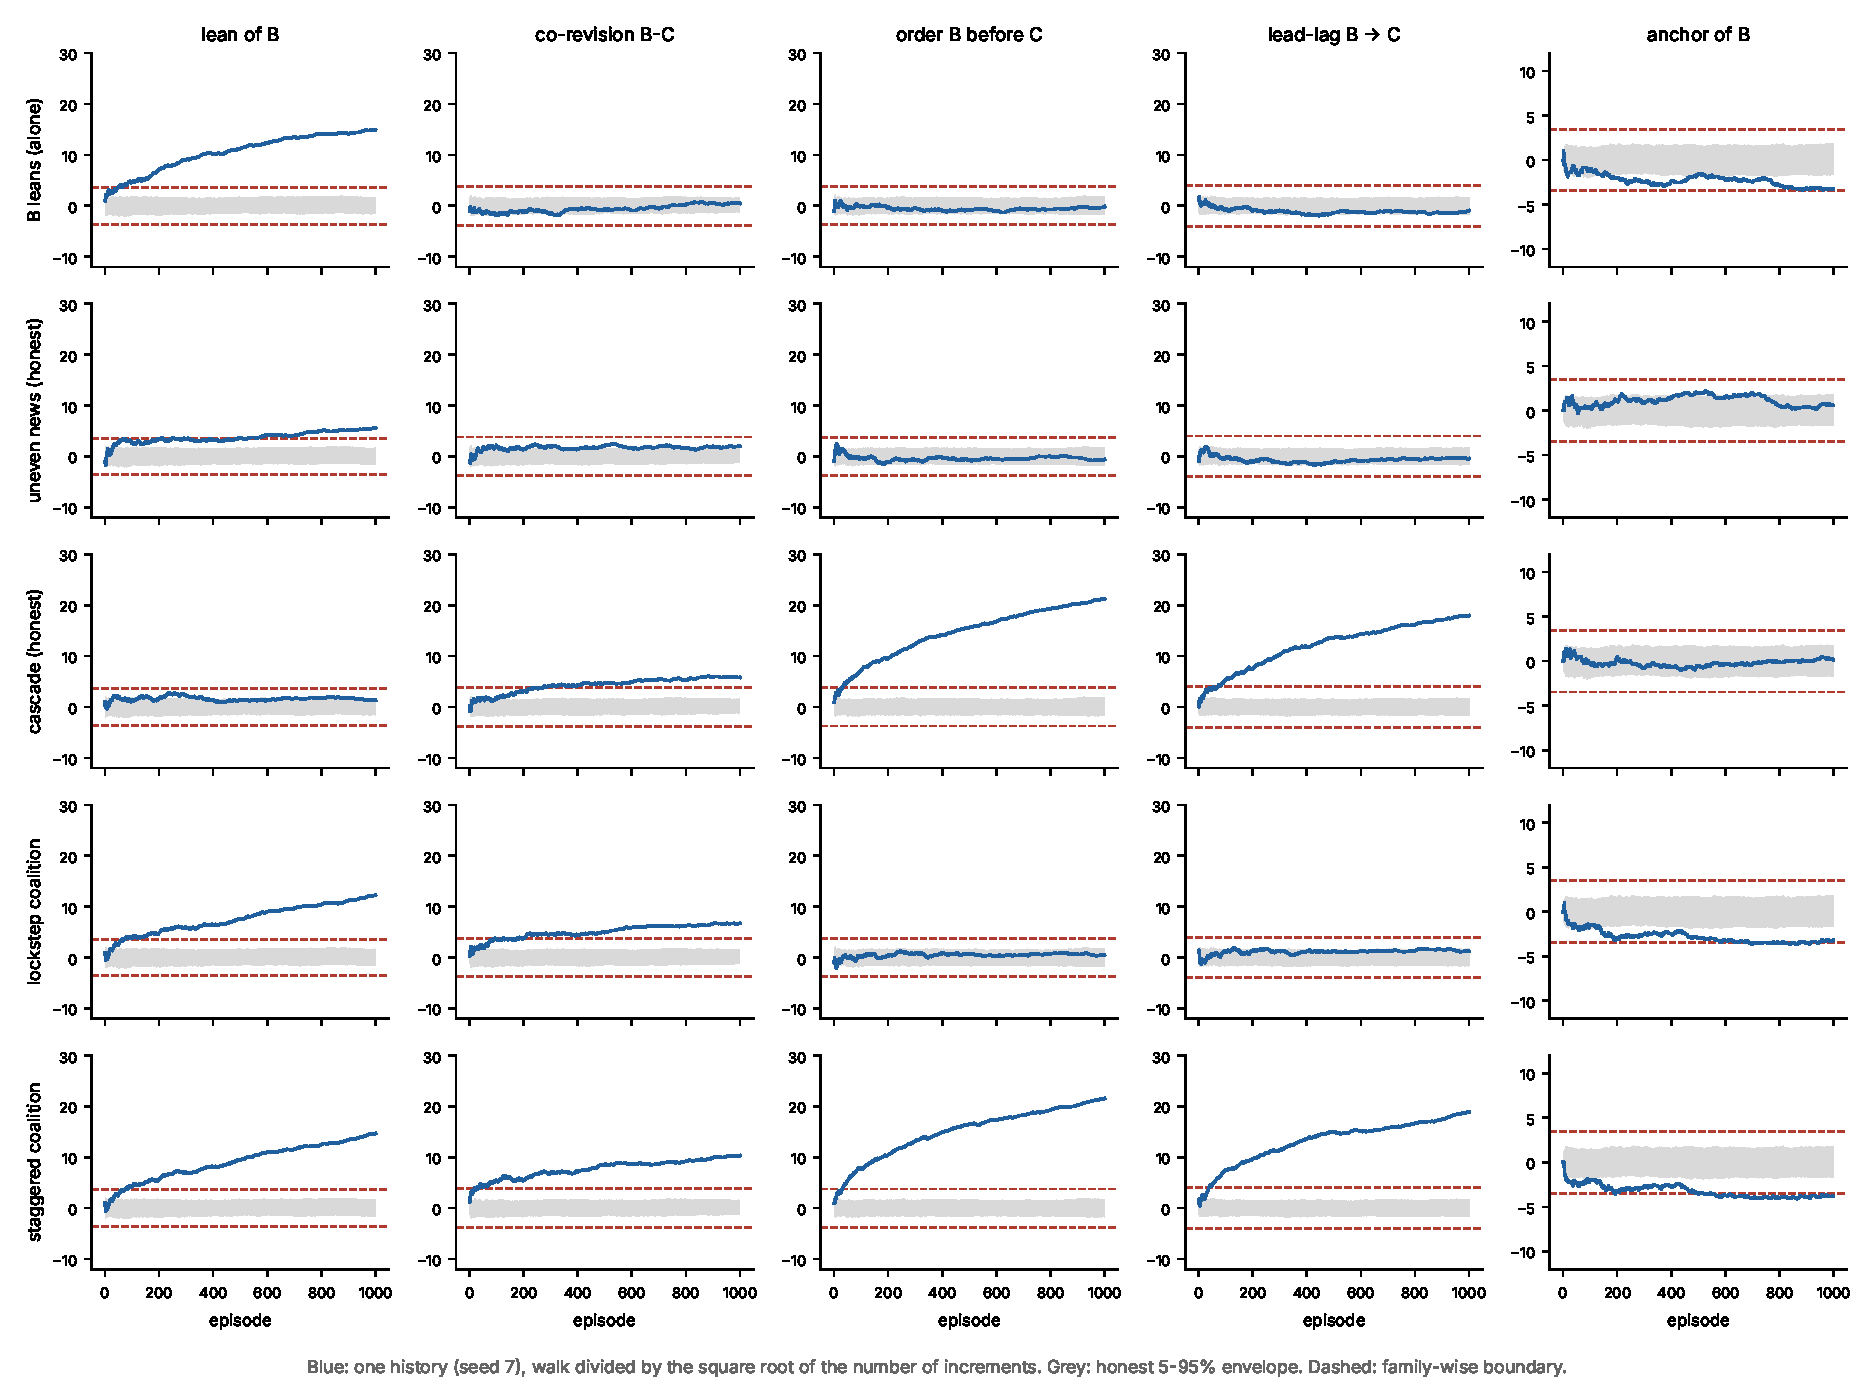
\includegraphics[width=\linewidth]{fig_memory_walks.pdf}
\caption{The five walks of $B$ and of the pair $B,C$ over $1000$ episodes, for one history of each condition (seed $7$). Each walk is divided by the square root of its number of increments. Grey: the $5$--$95\%$ envelope of $200$ honest histories. Dashed: the family-wise boundary.}\label{fig:memwalks}
\end{figure}
\begin{figure}[!htbp]\centering
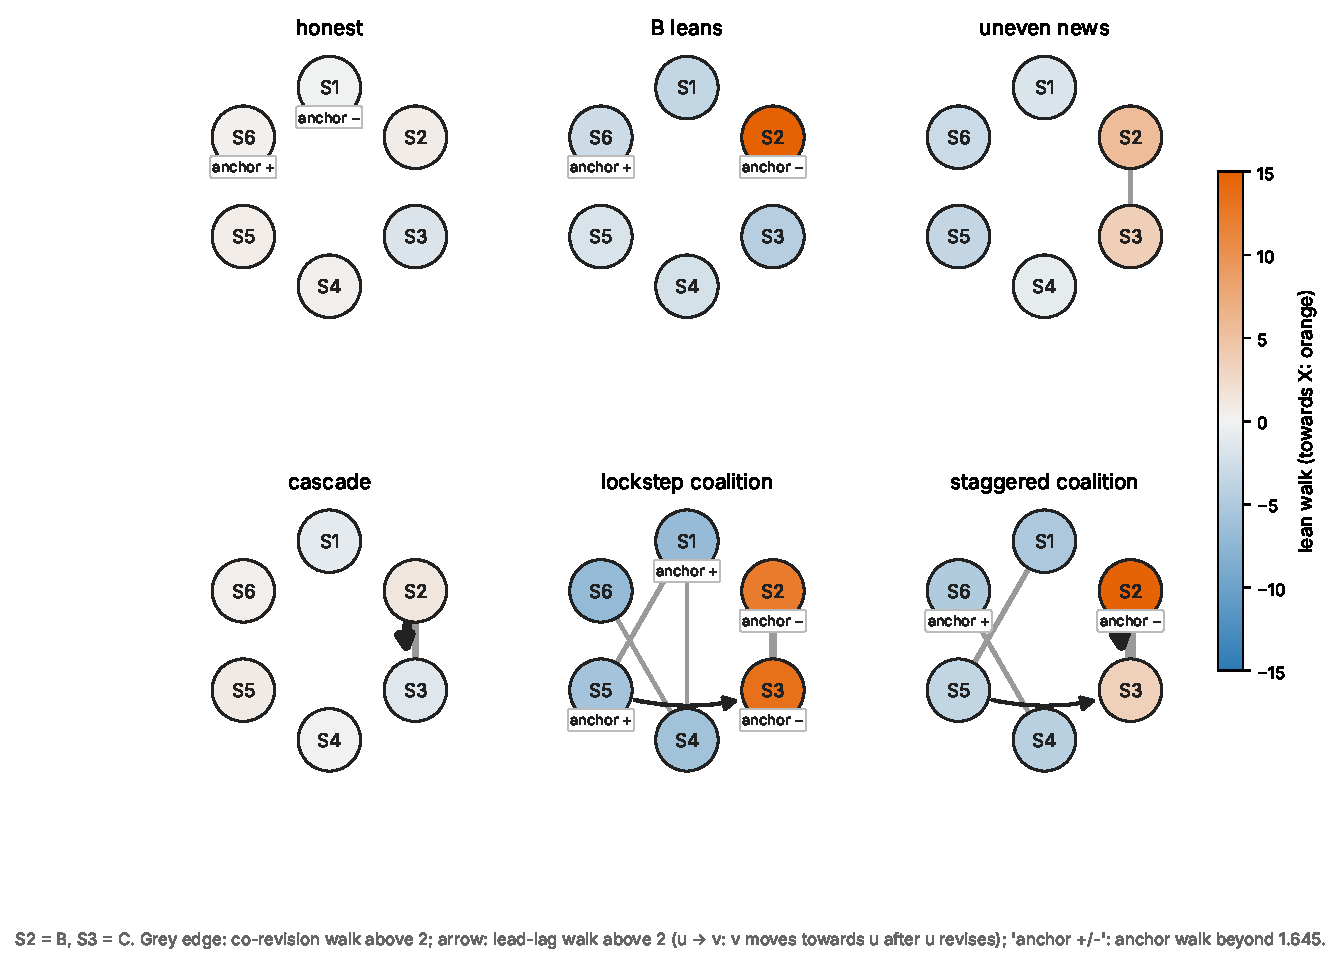
\includegraphics[width=0.95\linewidth]{fig_memory_network.pdf}
\caption{The decision maker's relation network after $1000$ episodes, one history per condition. Node colour is the lean walk (orange towards $X$, blue away). A grey edge is a co-revision walk above $2$. An arrow $u\to v$ is a lead-lag walk above $2$ ($v$ moves towards $u$ after $u$ revises). ``anchor $\pm$'' marks an anchor walk beyond $1.645$. Edges and labels here are descriptive and below the family-wise boundaries.}\label{fig:memnet}
\end{figure}

Across $200$ histories per condition, the share with an alarm in each family is as follows. Intervals are $95\%$ Wilson; the median alarm episode is given where alarms are common.
\begin{center}\footnotesize
\begin{tabular}{@{}lccccc@{}}
\toprule
condition & lean & co-revision & order & lead-lag & anchor\\\midrule
honest & $.05$ $[.03,.09]$ & $.04$ $[.02,.07]$ & $.07$ $[.04,.11]$ & $.04$ $[.02,.08]$ & $.06$ $[.03,.10]$\\
bias & $1.00$ (ep.\ 47) & $.06$ & $.07$ & $.05$ & $.26$\\
news (shared exactly) & $.04$ & $.04$ & $.04$ & $.05$ & $.04$\\
exposure (honest, uneven) & $1.00$ (ep.\ 334) & $.10$ & $.05$ & $.04$ & $.14$\\
cascade (honest) & $.04$ & $1.00$ (ep.\ 258) & $1.00$ (ep.\ 28) & $1.00$ (ep.\ 39) & $.13$\\
lockstep coalition & $1.00$ (ep.\ 44) & $1.00$ (ep.\ 214) & $.03$ & $.03$ & $.33$\\
staggered coalition & $1.00$ (ep.\ 44) & $1.00$ (ep.\ 133) & $1.00$ (ep.\ 28) & $1.00$ (ep.\ 39) & $.29$\\
\bottomrule
\end{tabular}
\end{center}
Some conditions are matched on purpose. The cascade and the staggered coalition have the same order rate ($B$ before $C$ in excess by $0.70$ per episode in both) and the same lead-lag rate ($0.59$ and $0.58$). The lockstep and staggered coalitions have similar leans for $B$ ($0.41$ and $0.49$ per episode). What separates them is the content: $B$'s lean ($0.00$ in the cascade, $0.49$ in the staggered coalition) and $B$'s anchor walk ($+0.09$ and $-0.15$ per anchored episode).

\paragraph{What the decision maker can conclude.}
\begin{itemize}
\item \emph{The three levels of evidence separate.} An \emph{individual} lean (bias) fires the lean walk alone. A \emph{relational} dependence without fixed order (lockstep) fires lean and co-revision, but not order or lead-lag. An \emph{ordered relational} pattern (cascade, staggered) fires order and lead-lag. Only the last kind of evidence motivates the ordered constructions of \cref{sec:ordrev}.
\item \emph{An honest cascade and a coalition look the same to every relational walk.} After a lead-lag alarm names a leader, a single follow-up test on the leader's anchor walk at the horizon (one-sided, level $5\%$) told them apart. It said ``the leader hurts'' for $161$ of $200$ staggered coalitions and $1$ of $200$ cascades. It said ``the leader helps'' for $65$ cascades and no coalition. The rest were unclear. This is the anchor doing what \cref{thm:protect} says only it can do.
\item \emph{Honest sources with better access to news are flagged.} Under uneven exposure the lean walk fired in every history, on $B$ or $C$ in $88\%$. These are honest sources that learned of news towards $X$ more often. Co-revision fired in $10\%$. Both of their anchor walks were positive in $81\%$ of histories. The memory detects dependence on information, not intent, and here the anchor points the right way.
\item \emph{A coalition pulls the median, so bystanders look biased.} With a watch-list on the uninvolved $S_5,S_6$ (a misspecified prior), the lean walk still fired in every staggered history. It fired on $S_5$ or $S_6$, always with the sign ``away from $X$'' ($200$ of $200$). Centred statistics spread a coalition's effect onto everyone else, which is one more reason never to read a single walk as an accusation.
\end{itemize}

\paragraph{Forgetting and priming.} A coalition that starts at episode $600$ is diluted by the walks that never forget. The discounted walks ($\lambda=0.99$, calibrated separately, with false-alarm rates between $4\%$ and $6.5\%$) flagged its lean, order and lead-lag at median episodes $677$, $652$ and $669$, against $800$, $742$ and $778$ (DL7). Priming was tested four ways (DL8).
\begin{itemize}
\item \emph{A correct watch-list supplied independently of the data} (the relations of $B$ and $C$) flagged the staggered coalition earlier: lean at $36$, order at $16$, lead-lag at $26$, against $44$, $28$ and $39$. Its honest false-alarm rates stayed between $2.5\%$ and $7\%$.
\item \emph{A misspecified watch-list} missed the order and lead-lag entirely, and produced the bystander alarms above.
\item \emph{A watch-list chosen from the same history}, by taking the strongest-looking relation and then testing it as if it had been declared in advance, raised the honest false-alarm rate to between $13.5\%$ and $28\%$. That is the cost of using the evidence twice.
\end{itemize}

\paragraph{The memory's state.} Putting the pieces together, and adding the record of how probabilities were combined (\cref{sec:poolcond}), the decision maker's private memory at episode $t$ is
\[
M_t=(\text{ledger};\;L_t,\;C_t,\;O_t,\;Q_t,\;A_t).
\]
The ledger is the source of truth. $L_t$ holds the leans, $C_t$ the co-revisions, $O_t$ the ordered relations (order and lead-lag walks, and the event braid or trace class of \cref{prop:ordrev} where (E1)--(E3) hold), $Q_t$ the operations of pooling and conditioning with their defects, and $A_t$ the anchors and their walks. The first four point; only the anchors decide.

\subsection{Pooling and conditioning}\label{sec:poolcond}
How a decision maker combines his sources is itself a sequence of operations, and their order can matter. Write $\mathcal P_w$ for pooling with weights $w$ and $\mathcal C_E$ for conditioning on evidence $E$. In general $\mathcal C_E\mathcal P_w\ne\mathcal P_w\mathcal C_E$, and the question is exactly when, and by how much.

\begin{proposition}[pooling and conditioning]\label{prop:poolcond}
Let sources $P_1,\dots,P_n$ on a finite space each assign the evidence $E$ the probability $P_i(E)>0$, and let $w$ be weights summing to $1$.
\begin{enumerate}
\item[(i)] For the linear pool $\mathcal P_w=\sum_iw_iP_i$, conditioning the pool equals pooling the conditioned sources with the weights $w_i'=w_iP_i(E)/\sum_jw_jP_j(E)$. Hence, with fixed weights, linear pooling and conditioning commute for $E$ exactly when the $P_i(E)$ with $w_i>0$ are all equal \cite{Stone1961,GenestZidek1986}.
\item[(ii)] The geometric pool $\prod_iP_i^{w_i}$, normalised, commutes with conditioning: it is externally Bayesian \cite{GenestMcConwaySchervish1986}. If the sources condition on different likelihoods $\ell_i$, the pool of their posteriors is the pool conditioned on $\prod_i\ell_i^{w_i}$.
\item[(iii)] The decision maker's own operation in this note, intersecting the fibres of the cells he trusts, does not depend on their order.
\end{enumerate}
\end{proposition}

\begin{proof}
(i) $\mathcal C_E\big(\sum_iw_iP_i\big)(x)=\sum_iw_iP_i(x)\mathbf 1_E(x)/\sum_jw_jP_j(E)=\sum_iw_i'\,\mathcal C_EP_i(x)$. The two sides agree for fixed $w$ exactly when $w'=w$ on the support of $w$, that is, when the $P_i(E)$ agree there. (ii) $\prod_i(P_i\ell_i)^{w_i}=\big(\prod_iP_i^{w_i}\big)\prod_i\ell_i^{w_i}$, and normalising commutes with multiplying by a common factor. (iii) Intersection is commutative and associative.
\end{proof}

So the ``defect'' of linear pooling is precisely a reweighting of the sources by how well each predicted the evidence. The numerical example that motivated this subsection has no defect, and (i) says why. With $P_A(X)=0.9$ and $P_B(X)=0.1$, and likelihoods $(0.9,0.1)$ for $A$ and $(0.1,0.9)$ for $B$, both sources give $E$ probability $0.82$. If $B$'s likelihoods are changed to $(0.3,0.6)$, then $P_B(E)=0.57$, the weights become $(0.59,0.41)$, and pooling first gives $P(X\mid E)=0.604$ against $0.520$ for conditioning first, a total-variation defect of $0.084$. PC1--PC4 in \texttt{engine/check\_poolcond.py} check (i)--(iii) on $300$ random cases each.

\paragraph{A manipulation channel.} Part (i) has a sharp consequence for poisoning. A decision maker who pools first and then conditions on each new item, as Bayesian model averaging does, gives weight to whichever source best \emph{predicted} the items. A source that also plants the items it predicts captures the weight. \Cref{fig:poolcond} shows a stream of $40$ items in which $X$ is false, generated by \texttt{engine/pce/poolcond.py}. Two honest sources and a third source $K$ start with equal weight. Every second item is a planted record that $K$'s model predicts with probability $0.9$ and the honest models with $0.3$, and that $K$ reads as favouring $X$.
\begin{itemize}
\item \emph{Pool, then condition:} $K$'s weight goes to $1$ within ten items, and the pooled $P(X)$ goes to $1$.
\item \emph{Condition, then pool with fixed weights:} $P(X)$ ends at $0.355$, held down by $K$'s fixed third.
\item \emph{Geometric pooling:} $P(X)$ ends at $0.842$, because $K$'s own posterior becomes extreme and the logarithmic pool follows extremes.
\item \emph{Without planting:} all three end near $0.005$, and $K$'s weight at $0.22$.
\end{itemize}
PC5 checks these values. The order of operations is therefore part of what the memory must keep. $Q_t$ records, for every step, the pooling rule, the weights, the evidence, and the defect. A source whose weight rises only on items no anchor ever verified is exactly the pattern above.
\begin{figure}[!htbp]\centering
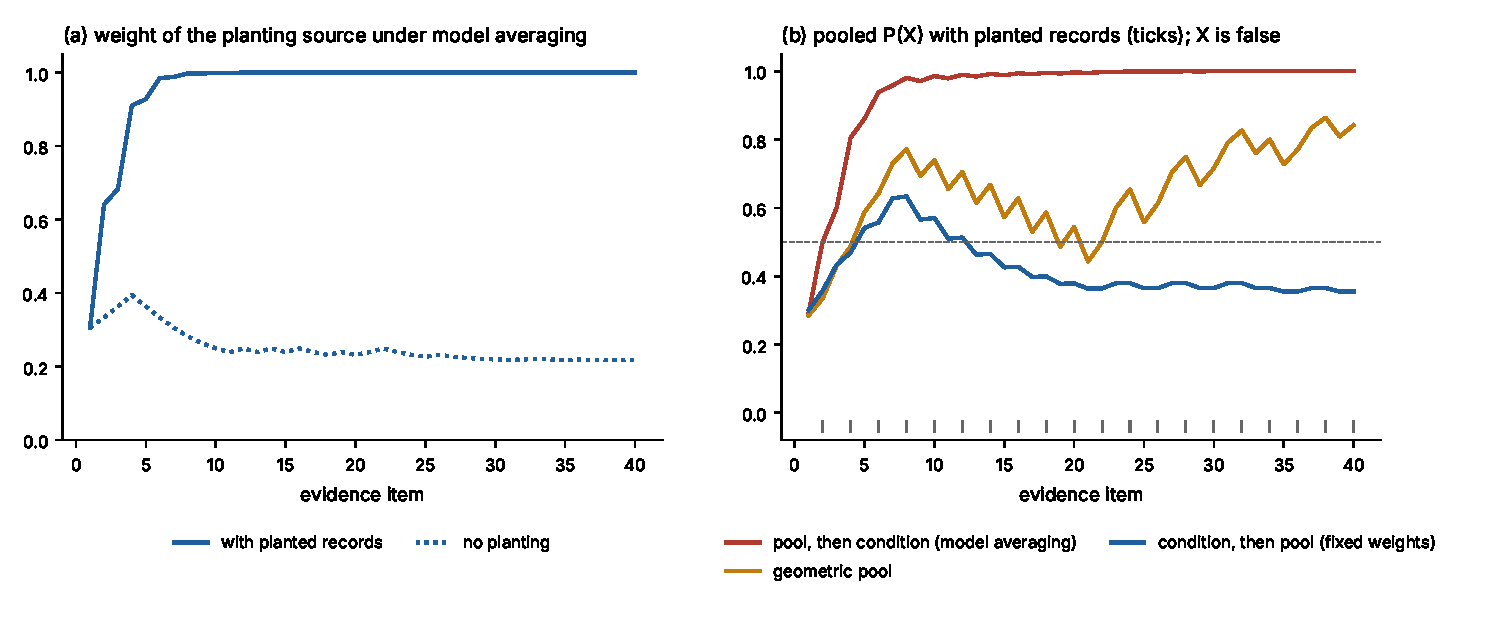
\includegraphics[width=\linewidth]{fig_poolcond.pdf}
\caption{Planted evidence and the order of pooling and conditioning. (a) The weight of the planting source $K$ under Bayesian model averaging, with and without planted records. (b) The pooled probability of $X$, which is false, under three ways of combining, with planted records marked by ticks.}\label{fig:poolcond}
\end{figure}

Non-commuting operations do not by themselves give a braid. A braid representation needs generators that also satisfy $\sigma_i\sigma_{i+1}\sigma_i=\sigma_{i+1}\sigma_i\sigma_{i+1}$, and nothing here provides that. We record the operations as a sequence in $Q_t$, not as a braid.


\section{Three-dimensional fibres}\label{sec:twofour}
A $2\times3$ fibre is a polygon, so selection has at most two levels. A $2\times4$ fibre $\mathrm{Cpl}(f,g)$ is a three-dimensional polytope, and the leximin recursion can cut it down in up to three
steps: a sheet, then a line, then a point. This part asks what such a deeper hierarchy does on the other side, and it keeps three questions apart. Is the chamber Fano, so that the Floer layer of
\cref{sec:floer} applies? How many dimensions does each level remove? And does the Clifford form of the positive object see each level? The answers are, in order: only $14$ of the $148$ chambers are
Fano, and in those coupled three-step selection never occurs (\cref{thm:chambers24,prop:fanodepth}); a level can remove more than one dimension; and in every example the Clifford form has one scale
per removed dimension (\cref{conj:leveldrop}, proved at leading order in three examples).

\subsection{Coordinates and the potential}
Use $u=(a_{11},a_{12},a_{13})$. The eight cells are $a_{1j}=u_j$ and $a_{2j}=g_j-u_j$ for $j\le3$, $a_{14}=f_1-\sum_ju_j$, and $a_{24}=\sum_ju_j-(f_1+g_1+g_2+g_3-1)$. Their normals are $\pm e_j$ and
$\mp(1,1,1)$. Over the facet cells (a non-facet cell contributes no term), the potential is
\begin{equation}\label{eq:W24}
W=\sum_{j\le3}\Bigl([1j]\,y_j+[2j]\,\frac{T^{g_j}}{y_j}\Bigr)+[14]\,\frac{T^{f_1}}{P}+[24]\,T^{g_4-f_1}P,\qquad P=y_1y_2y_3,
\end{equation}
where $[ij]=1$ if cell $ij$ is a facet and $0$ otherwise. For each example we keep three counts separate: the vertices of the fibre (equal to $\chi(X)$), the critical points of $W$, and the distinct
fibres that carry them.

\subsection{Ampleness, certified by curves}
Whether $X_{(f,g)}$ is Fano is a statement about its fan, and so about the chamber of $(f,g)$. We certify it with integers on the edges of the polytope, by a classical criterion, rather than by
any probabilistic argument.

\begin{proposition}[ampleness by curves]\label{prop:kleiman}
Let $X$ be a smooth complete toric threefold with polytope $Q$.
\begin{enumerate}
\item[(1)] (Nakai--Moishezon) A divisor $D$ on a projective variety is ample if and only if $D^{\dim V}\cdot V>0$ for every irreducible subvariety $V$ of positive dimension \cite{Kleiman1966}.
\item[(2)] (toric Kleiman) On a complete toric variety it suffices to test the torus-invariant curves: $D$ is ample if and only if $D\cdot C>0$ for each of them, and nef if and only if $D\cdot C\ge0$
\cite[Theorem~6.3.13 and \S6.3]{CLS2011}.
\item[(3)] The invariant curves are the edges of $Q$. If an edge lies on the facets $i,j$ and joins the vertices whose third facets are $k$ and $l$, the wall relation $v_k+v_l+a\,v_i+b\,v_j=0$ has
integer $a,b$, and $D_k\cdot C=D_l\cdot C=1$, $D_i\cdot C=a$, $D_j\cdot C=b$, and $D_\rho\cdot C=0$ otherwise \cite[\S6.4]{CLS2011}. So $-K\cdot C=2+a+b$, and the K\"ahler class meets $C$ in
$-\lambda_k-\lambda_l-a\lambda_i-b\lambda_j$, which must equal the lattice length of the edge.
\end{enumerate}
On a toric variety $-K$ is always big, since its polytope $\{m:\langle m,v_\rho\rangle\ge-1\}$ contains $0$ in its interior. So nef already means weak Fano.
\end{proposition}

Part (3) contains its own test: the lattice length of every edge must come out of the same integers that give $-K\cdot C$. TF2 confirms it on all $2208$ edges of all chambers. The curves with
$-K\cdot C=0$ matter twice. They are what makes a chamber weak Fano rather than Fano. And they span the anticanonically trivial directions of the Mori cone, so they are the geometric source of the classes that \emph{may} contribute to the corrections of $W$ (\cref{rem:corrections}); a zero degree does not by itself give a nonzero contribution.

\begin{theorem}[the $2\times4$ chambers]\label{thm:chambers24}
The nondegenerate $2\times4$ margins fall into $148$ K\"ahler chambers, the sign patterns of $f_1-g(J)$ over the $14$ nonempty proper sets $J$ of columns. Every chamber polytope is simple and smooth.
By \cref{prop:kleiman} they are of six types:
\begin{center}\footnotesize\setlength{\tabcolsep}{4pt}
\begin{tabular}{lcccccccl}\toprule
type & chambers & facets & $\chi$ & $(-K)^3$ & curves with $-K\cdot C=0$ & $W$ & Floer reading & drop patterns seen\\\midrule
$\mathbb{CP}^3$ & $2$ & $4$ & $4$ & $64$ & $0$ & as is & Cho--Oh & $(3)$\\
$\mathrm{Bl}_{pt}\mathbb{CP}^3$ & $8$ & $5$ & $6$ & $56$ & $0$ & as is & Cho--Oh & $(3)$, $(1,2)$\\
$(\mathbb{CP}^1)^3$ & $4$ & $6$ & $8$ & $48$ & $0$ & as is & Cho--Oh & $(1,1,1)$, decoupled\\
weak Fano & $24$ & $6$ & $8$ & $48$ & $1$ & $(1+\delta_k)$ & withheld & $(3)$, $(1,2)$, $(1,1,1)$\\
weak Fano & $64$ & $7$ & $10$ & $40$ & $3$ & $(1+\delta_k)$ & withheld & $(3)$, $(1,2)$, $(1,1,1)$\\
weak Fano & $46$ & $8$ & $12$ & $32$ & $6$ & $(1+\delta_k)$ & withheld & $(3)$, $(1,2)$, $(1,1,1)$\\\bottomrule
\end{tabular}
\end{center}
Here $\chi$ is also the number of vertices, and ``$(1+\delta_k)$'' means the corrections of \cref{rem:corrections}.
In every chamber the normalised volume of $\operatorname{conv}\{v_c\}$ over the facets equals the number of vertices. The $148$ are chambers of the margin hyperplane arrangement only: leximin walls
subdivide them further, so the drop pattern is not a chamber invariant, and the last column lists only the patterns seen in a census.
\end{theorem}

\begin{proof}
An exact computation, TF1--TF3, with a machine-readable certificate, the file \texttt{chambers24.json} in \texttt{kahler/}, and an independent verifier (CC1--CC4). Each of the $148$ chambers is certified by an exact rational interior point; that no other sign pattern is realised rests on linear-programming infeasibility. For each
chamber, $-K\cdot C$ is computed on every edge from the integer wall relation, the type is read from the primitive relations, and an independent anticanonical vertex test agrees in all $148$. The
drop patterns are not invariants of a K\"ahler chamber, because leximin walls subdivide it; the last column lists those seen in a tie-free census (TF8).
\end{proof}

\begin{proposition}[the box, and selection depth in the Fano chambers]\label{prop:fanodepth}
\begin{enumerate}
\item[(1)] $\mathrm{Cpl}(f,g)$ is a box exactly when some column has $g_j>\max(f_1,f_2)$. Then column $j$ never binds, $X=(\mathbb{CP}^1)^3$, $W$ is a sum of three $\mathbb{CP}^1$ potentials, and the levels are
the half-masses $g_k/2$ of the other three columns.
\item[(2)] In a $\mathbb{CP}^3$ chamber selection is immediate: pattern $(3)$. In a $\mathrm{Bl}_{pt}\mathbb{CP}^3$ chamber it is $(3)$ or $(1,2)$.
\end{enumerate}
So coupled selection in three steps occurs only in weak Fano chambers.
\end{proposition}

\begin{proof}
(1) The column-$j$ inequalities $0\le f_1-\sum_{k\ne j}a_{1k}\le g_j$ hold on the whole box $0\le a_{1k}\le g_k$ exactly when $1-g_j\le f_1\le g_j$. Then the two cells of column $j$ are not facets and their terms do not appear in \eqref{eq:W24}. Each remaining column contributes
$y+T^{g}/y$ in its own coordinate: $y_k$ for a column $k\le3$, and $z=T^{f_1}/P$ for column $4$. These three coordinates are a unimodular basis. (2) By TF4 the facets of a $\mathbb{CP}^3$ chamber are one full row $i$, so the fibre is
the simplex $\{a_{i\cdot}\ge0,\ \sum_ja_{ij}=f_i\}$ and the equal split $f_i/4$ is selected at once. The facets of a $\mathrm{Bl}_{pt}\mathbb{CP}^3$ chamber are one full row $i$ and one cell $i'j$, which cuts off a
corner. If $f_i/4<g_j/2$ the equal split is still selected at once. Otherwise column $j$ binds first, at $g_j/2$, and the remaining three cells of row $i$ share $f_i-g_j/2$ equally at the second level, a
drop of two.
\end{proof}

A binding row finishes selection, since it leaves a candidate set of dimension $(n-2)(m-1)=0$. The counting formula of \cref{thm:maxmincoupling} gives only the first level, and the examples show
that later levels can remove one or two dimensions. Write $r_j$ for the number of dimensions removed at level $j$, the rank increment of the fixed normals; a level can also remove none, as the last
level of example C does.

\begin{figure}[!htbp]\centering
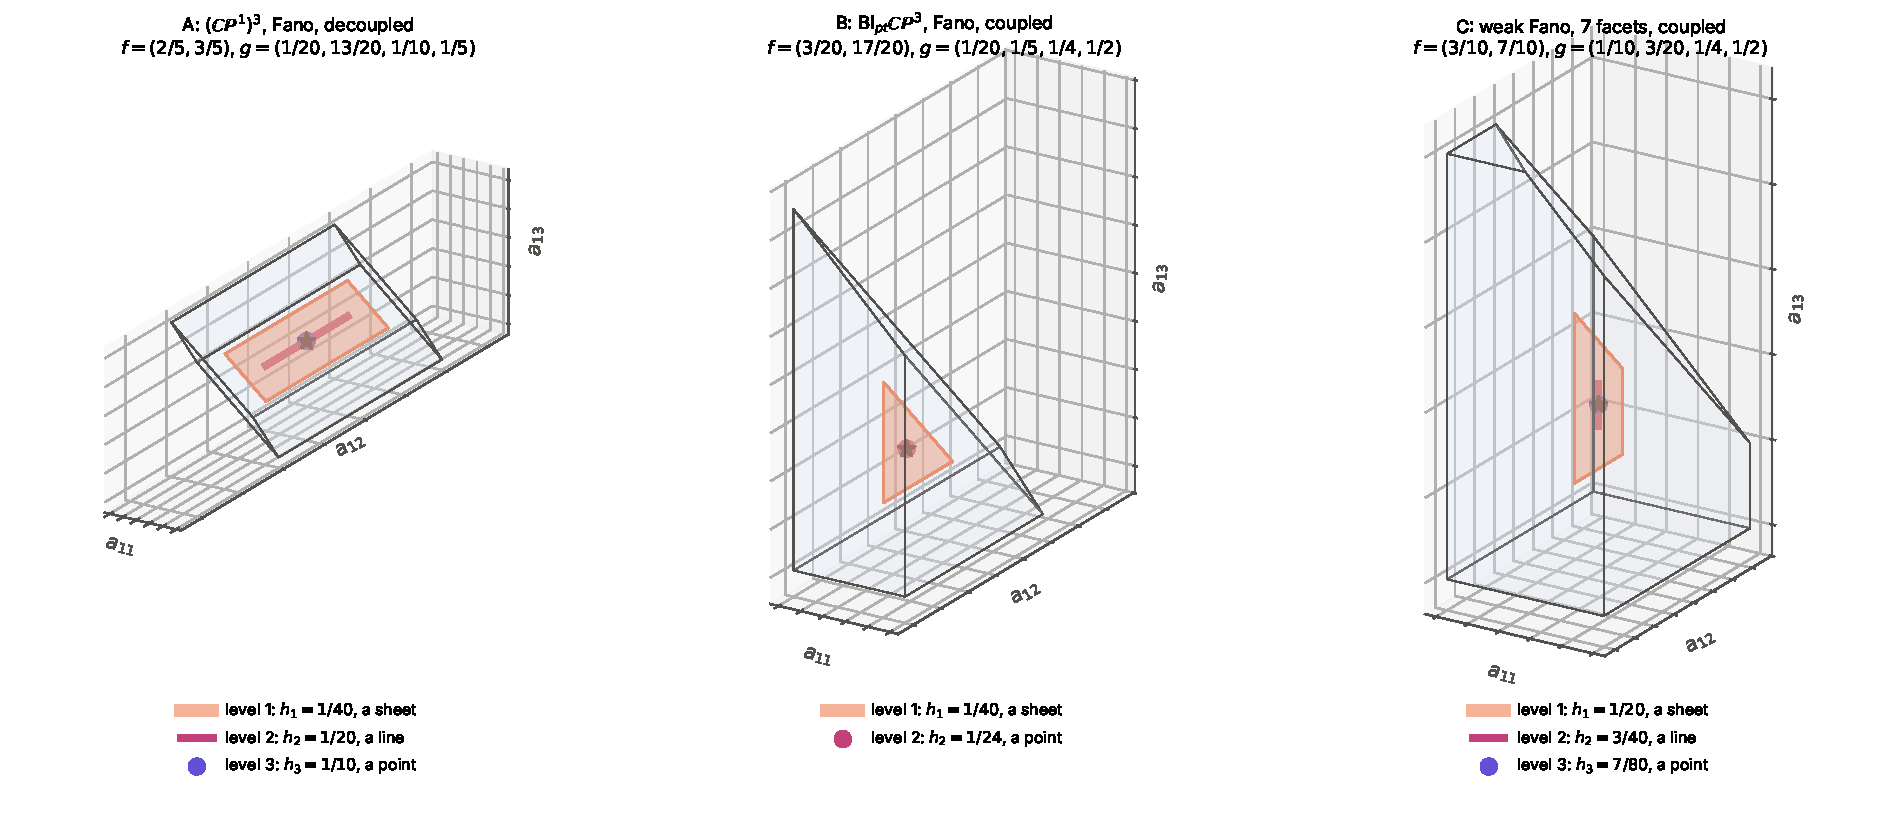
\includegraphics[width=\linewidth]{fig_tf_polytopes.pdf}
\caption{The three fibres and their candidate sets. Orange: the sheet left by the first level (a binding column). In A and C the second level leaves a line and the third a point; in B the second level
is a binding row on what is left, and it fixes two dimensions at once. The star is the leximin point, the valuation of the positive critical point (\cref{thm:selection}).}\label{fig:tfpoly}
\end{figure}

\subsection{Three examples}
\begin{example}[A: the box]\label{ex:A24}
Take $f=(2/5,3/5)$ and $g=(1/20,13/20,1/10,1/5)$. Column $2$ never binds, so by \cref{prop:fanodepth}(1) the fibre is a box, $X=(\mathbb{CP}^1)^3$, and $W=(y_1+T^{1/20}/y_1)+(y_3+T^{1/10}/y_3)+(z+T^{1/5}/z)$
with $z=T^{2/5}/P$. The levels are $1/40$, $1/20$, $1/10$, with drops $(1,1,1)$. The $8$ critical points are $y_1=\pm T^{1/40}$, $y_3=\pm T^{1/20}$, $z=\pm T^{1/10}$, all over the leximin fibre
$(1/40,9/40,1/20)$, with leading holonomies $\pm1$. Their critical values are $2(\pm x\pm x^2\pm x^4)$ with $x=T^{1/40}$. For $T\in(0,1)$ exactly two coincide, $(+,-,-)$ and $(-,+,+)$, at the root of
$x^3+x-1=0$, $T^*\approx2.3\times10^{-7}$. There the $m_0$ argument for vanishing Hom does not apply (the holonomies still differ), and we do not compute that group. TF5 checks all of this exactly.
\end{example}

\begin{proposition}[B: the blown-up projective space, exactly]\label{prop:B24}
Take $f=(3/20,17/20)$ and $g=(1/20,1/5,1/4,1/2)$. The facets are row $1$ and cell $21$, so $X=\mathrm{Bl}_{pt}\mathbb{CP}^3$ and $W=y_1+y_2+y_3+T^{3/20}/P+T^{1/20}/y_1$. Put $\tau=T^{1/20}$.
\begin{enumerate}
\item[(1)] \emph{Selection.} Column $1$ binds at $h_1=1/40$, and row $1$ then spreads $1/8$ over three cells, $h_2=1/24$. The drops are $(1,2)$.
\item[(2)] \emph{Reduction.} At a critical point $y_2=y_3=c$ and $y_1=\tau^3/c^3$, where $c^6+\tau^2c^4-\tau^5=0$. As a cubic in $c^2$ this has discriminant $\tau^{10}(4\tau-27)$, so there are $6$ distinct
critical points for $T\in(0,1)$.
\item[(3)] \emph{One fibre.} The Newton polygon of the cubic has a single edge. All six critical points lie over the leximin fibre $(1/40,1/24,1/24)$, with $c=\zeta T^{1/24}(1+o(1))$ and
$y_1=\zeta^{-3}T^{1/40}(1+o(1))$, $\zeta^6=1$.
\item[(4)] \emph{Distinct values.} The critical values $w=2y_1+2c$ are the roots of a sextic whose discriminant is $2^{36}\tau^{19}(4\tau-27)^6(4\tau+1)^2$. So they are distinct for every $T\in(0,1)$.
\item[(5)] \emph{Objects and morphisms} (Fano; cited, in the convention of \cref{sec:cbclass}). The six are objects over one fibre, with distinct $m_0$, so every off-diagonal Hom vanishes and the
category they generate is $\bigoplus_{c=1}^6\mathrm{Cl}(Q_c)$ over $\Lambda$, with no higher products. Generation is conditional.
\end{enumerate}
\end{proposition}

\begin{proof}
(1) By \cref{prop:fanodepth}(2), since $f_1/4=3/80>g_1/2=1/40$. (2) The equations $y_j\partial_jW=0$ give $y_2=y_3=T^{3/20}/P=c$ and $y_1-\tau/y_1=c$; eliminating gives the sextic, and the
discriminant follows. (3) The lower hull of $(3,0),(2,2),(0,5)$ in the plane of (power of $c^2$, power of $\tau$) is the single segment from $(0,5)$ to $(3,0)$, of slope $-5/3$, so
$c^2\sim\tau^{5/3}$ and $c\sim\tau^{5/6}=T^{1/24}$. Then $y_1=\tau^3/c^3$. (4) A resultant. (5) \Cref{prop:morph}(2)--(3) and \cref{prop:formal}, with (4). TF6 checks (2)--(4) symbolically.
\end{proof}

\begin{example}[C: weak Fano, coupled in three steps]\label{ex:C24}
Take $f=(3/10,7/10)$ and $g=(1/10,3/20,1/4,1/2)$. The facets are row $1$ and cells $21,22,23$, so seven facets, and the chamber is weak Fano with three curves of $-K\cdot C=0$. Here
$W=\sum_{j\le3}(y_j+T^{g_j}/y_j)+T^{3/10}/P$. Columns $1$ and $2$ bind in turn, at $h_1=1/20$ and $h_2=3/40$. Row $1$ then spreads $7/40$ over cells $13$ and $14$, at $h_3=7/80$. The last cell, $23$,
is fixed at $13/80$ without removing a dimension. The drops are $(1,1,1,0)$. The critical equations reduce to one resultant of degree $10$ in $c=T^{3/10}/P$, even in $c$. Its Newton polygon in $c^2$
has an edge of slope $7/2$ with four roots and one of slope $1$ with one root. So $8$ critical points lie over the leximin fibre $(1/20,3/40,7/80)$, with leading holonomies of the form
$(\pm1,\pm1,\pm1)$ or $(\pm1,\pm1,\pm i)$, and $2$ lie over $(1/40,1/40,9/40)$, with holonomies $\pm(i,i,i)$. On that second fibre the leading set is $\{11,12,14,23\}$, with leading coefficients
$\rho=(i,i,i,-i)$ up to conjugation. (H1) holds and (H2) fails, yet $\operatorname{rank}M_c=3=\dim\operatorname{span}$: two more instances of the equality in \cref{thm:reduction} without its sufficient
condition. TF7 and TF9 check this.
\end{example}

\begin{remark}[what changes in a weak Fano chamber]\label{rem:corrections}
For a semi-Fano toric manifold, that is, one with $-K$ nef, the potential of a fibre is $W^{\mathrm{LF}}=\sum_k(1+\delta_k)\,T^{-\lambda_k}y^{v_k}$, where
$\delta_k=\sum_{\alpha\ne0}n_{\beta_k+\alpha}T^{\omega(\alpha)}$ runs over the classes $\alpha$ of rational curves with $-K\cdot\alpha=0$ \cite[Proposition~2.15]{CLLT2020}. The monomials are the same and only the coefficients
change, by factors $1+O(T^\varepsilon)$. Three consequences, and one thing withheld:
\begin{enumerate}
\item[(i)] The valuations of the terms are unchanged, so the levels $h_j$, the leximin point and the leading coefficients are unchanged.
\item[(ii)] \Cref{thm:selection} needs real coefficients with uniform bounds. If the $\delta_k$ converge for small $T$, are real, and satisfy $0<c\le1+\delta_k(e^{-L})\le C$ for large $L$, then it applies
to $W^{\mathrm{LF}}$ as it stands: the corrected positive critical point is selected at the leximin point, with error $O(1/L)$. If the $\delta_k$ are only formal Novikov series, the conclusion holds as a
statement about valuations, by (i), and not about a real critical point.
\item[(iii)] The leading-order argument of \cref{prop:scales} uses only valuations and leading coefficients, so it applies to $W^{\mathrm{LF}}$ verbatim (argued, not checked).
\item[(iv)] Withheld: the exact critical points of $W^{\mathrm{LF}}$, their number over each fibre, and the Floer reading of the ten objects. We do not compute the $\delta_k$.
\end{enumerate}
For each curve with $-K\cdot C=0$ four statuses must be kept apart: zero anticanonical degree (computed here, exactly); an effective class $\alpha$ through it that contributes to some $\delta_k$ (not determined);
a nonzero invariant $n_{\beta_k+\alpha}$ (not computed); the correction evaluated (not done).
\end{remark}

\begin{figure}[!htbp]\centering
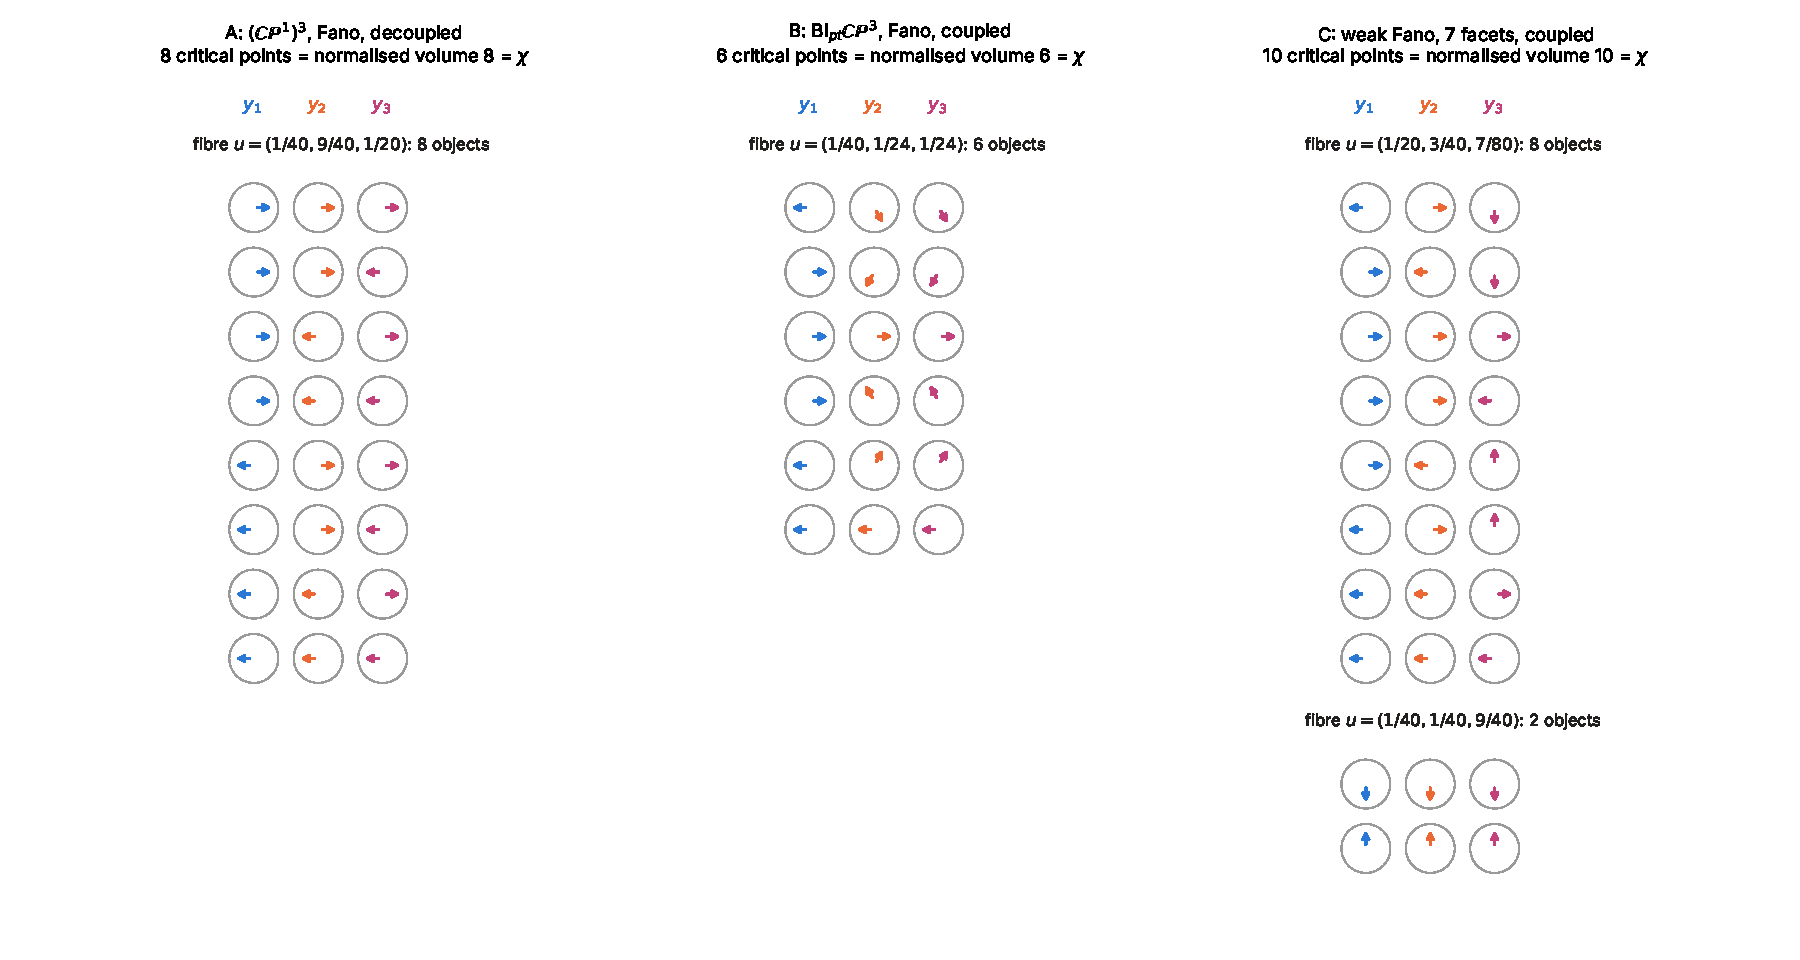
\includegraphics[width=\linewidth]{fig_tf_objects.pdf}
\caption{Every critical point of the three potentials, grouped by fibre, with its leading holonomies drawn as dials (the arrow is the phase of $y_j$). A and B have one fibre each. C has two: eight
points over the leximin fibre and two over $(1/40,1/40,9/40)$. In each case the number of critical points equals the normalised volume of the Newton polytope, which equals $\chi$, and that equality
certifies the list complete. For C these are the critical points of the uncorrected $W$ (\cref{rem:corrections}).}\label{fig:tfobjects}
\end{figure}

\subsection{One scale per removed dimension}
\Cref{thm:shadow} says that the reduction of $Q/W$ mod $T$ has rank $r_1$. The examples say more: the other directions of $Q/W$ have exact scales, one for each dimension a later level removes. To state
this without ordering eigenvalues, use determinantal divisors.

\begin{definition}[scale valuations]\label{def:scales}
For a matrix $M$ over $\Lambda_0$, let $d_k$ be the least valuation of a $k\times k$ minor, and $e_k=d_k-d_{k-1}$, with $d_0=0$. The $e_k$ are the valuations of the invariant factors of $M$. They do not
change under $M\mapsto AMB$ with $A,B\in\mathrm{GL}_n(\Lambda_0)$, in particular under a change of integral basis of $H^1(L;\mathbb Z)$.
\end{definition}

For the positive object, $Q/W$ is real symmetric and positive definite, and its scale valuations are the valuations of its eigenvalues. The sum of the $k\times k$ principal minors is the $k$-th
elementary symmetric function of the eigenvalues; all terms are positive, so its valuation is that of the product of the $k$ largest eigenvalues. And for a positive definite matrix
$|\det M_{IJ}|^2\le\det M_{II}\det M_{JJ}$, so the least valuation over all $k\times k$ minors is attained on a principal one.

\begin{conjecture}[one scale per removed dimension]\label{conj:leveldrop}
For nondegenerate margins, the scale valuations of $Q/W$ at the positive object are $0$ with multiplicity $r_1$, and $h_j-h_1$ with multiplicity $r_j$ for each later level $j$. A level that removes no
dimension contributes nothing.
\end{conjecture}

\begin{proposition}[the conjecture in the three examples]\label{prop:scales}
At leading order, the scale valuations of $Q/W$ are:
\begin{enumerate}
\item[(A)] $(0,\,1/40,\,3/40)$ for all $8$ objects;
\item[(B)] $(0,\,1/60,\,1/60)$ for all $6$ objects: the second level removes two dimensions and gives a double scale;
\item[(C)] $(0,\,1/40,\,3/80)$ for the $8$ objects over the leximin fibre, with no scale from the fourth level; and $(0,0,0)$ for the two over the second fibre.
\end{enumerate}
So \cref{conj:leveldrop} holds in A, B and C.
\end{proposition}

\begin{proof}
In every case $Q=\sum_k(\text{term }k)\,v_kv_k^{\!\top}$, and at a critical point $y_j-T^{g_j}/y_j=c$, where $c$ is the value of the $P$-term.
(A) In the unimodular basis $(\log y_1,\log y_3,\log z)$, $Q=\operatorname{diag}(W_1,W_3,W_z)$, with each factor's value $\pm2T^{h}$ and $W\sim\pm2T^{1/40}$.
(B) $Q=\left(\begin{smallmatrix}2y_1&c&c\\c&2c&c\\c&c&2c\end{smallmatrix}\right)$ and $W=2y_1+2c$, with $y_1\sim T^{1/40}$ and $c\sim T^{1/24}$ (\cref{prop:B24}). So $d_1=0$. The $2\times2$ minors have least valuation
$1/40+1/24$, attained by $4y_1c-c^2$, so $d_2=1/24-1/40=1/60$. Next, $\det Q=6y_1c^2-2c^3\sim T^{1/40+1/12}$, so $d_3=1/30$, and $e=(0,1/60,1/60)$.
(C) $Q=D+cJ$, with $J$ the all-ones matrix and $D=\operatorname{diag}(2y_j-c)$. On the leximin fibre $y_1\sim\pm T^{1/20}$, $y_2\sim\pm T^{3/40}$ and $c\sim y_3\sim T^{7/80}$, so
$D\approx\operatorname{diag}(2y_1,2y_2,y_3)$ and $W\approx2y_1$. The $2\times2$ minors have least valuation $1/20+3/40$, so $d_2=1/40$. Next,
$\det Q=D_1D_2D_3+c\,(D_1D_2+D_1D_3+D_2D_3)\approx 2y_3D_1D_2\sim T^{17/80}$, with no cancellation, so $d_3=17/80-3/20=1/16$, and $e=(0,1/40,3/80)$. The second fibre has rank $3$ by \cref{ex:C24}.
TF9 checks every case numerically: the eigenvalue slopes at the positive object, and the minors on every object over the leximin fibre. These finite-$T$ checks corroborate the limiting valuations;
the proof is the leading-order computation above.
\end{proof}

\begin{figure}[!htbp]\centering
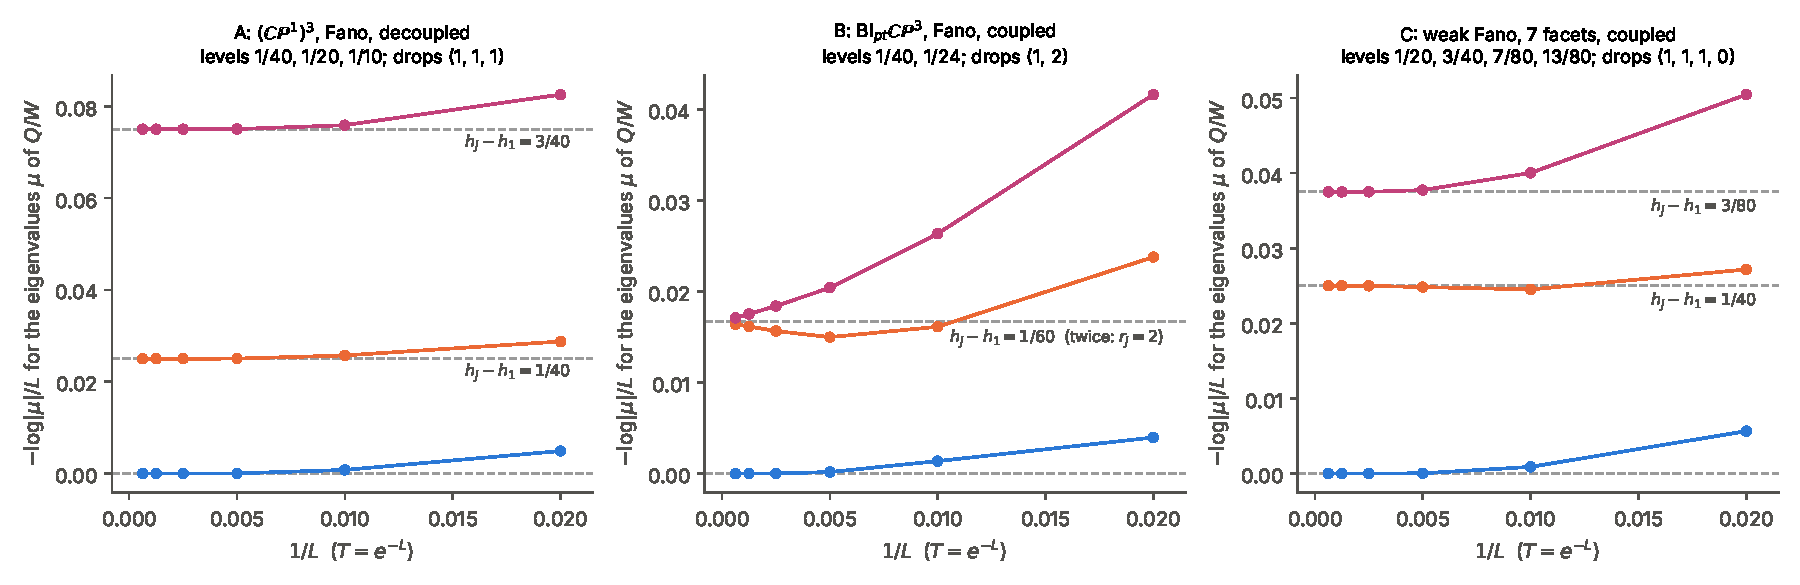
\includegraphics[width=\linewidth]{fig_tf_spectrum.pdf}
\caption{The eigenvalues of $Q/W$ at the positive object, as $-\log|\mu|/L$ against $1/L$ for $L=50,\dots,1600$. The finite-$T$ offset is linear in $1/L$, so the curves run straight into their
limits: $0$ once, then $h_j-h_1$ for each removed dimension. In B the second level removes two dimensions and two eigenvalues share the limit $1/60$. In C the fourth level, $13/80$, removes none and
leaves no trace.}\label{fig:tfspectrum}
\end{figure}

In $2\times3$ the evidence was single scales: $(3\alpha-1)/4$ on $F_1$, $1/200$ after one count, and $1/20$ in the column-binding example (\cref{sec:morph}). The cube proves the conjecture for every box
chamber, because the factors decouple. B is the first coupled case with a multiplicity, and C the first coupled case with three levels and a level that removes nothing. A proof in general would need
the successive balances of \cref{thm:selection} to appear, one order at a time, in the minors of $Q$. That is the step we have not found.


\subsection{Phases of the objects: Bloch spheres and holonomy groups}\label{sec:bloch}
Each object in \cref{fig:tfobjects} is drawn with three dials. Two pieces of information are attached to it. One is the torus fibre it lives on, whose position $u$ in the polytope is a coupling, that is, a probability law on the cells of the table. The other is the holonomy of its flat connection, a point $\theta$ of a three-dimensional torus, which the dials show. Probabilities and phases appearing together suggest the picture physicists use for a two-level system, the Bloch sphere, and this subsection asks how far that picture applies.

Recall the Bloch sphere. A two-outcome law $(1-p,p)$ together with a phase $\theta$ defines the unit vector $\psi=\sqrt{1-p}\,|0\rangle+\sqrt p\,e^{i\theta}|1\rangle$ in $\mathbb C^2$, up to an overall phase. Such vectors are the points of $\mathbb{CP}^1$, which is a round sphere. The height on the sphere is $1-2p$, so latitude records the probability, and the longitude is $\theta$. Explicitly, the point is
\[
\big(2\sqrt{p(1-p)}\cos\theta,\ 2\sqrt{p(1-p)}\sin\theta,\ 1-2p\big).
\]
The round metric splits accordingly. For $z=\sqrt p\,e^{i\theta}$ with any number of components, the Fubini--Study line element is
\[
ds^2_{\rm FS}=\tfrac14\sum_j\frac{dp_j^2}{p_j}+\sum_jp_j\,d\theta_j^2-\Big(\sum_jp_j\,d\theta_j\Big)^2 .
\]
The first term is a quarter of the Fisher--Rao metric, and the rest measures relative phase. To see this, write $dz_j=(dp_j/2\sqrt{p_j}+i\sqrt{p_j}\,d\theta_j)e^{i\theta_j}$, use $\sum dp_j=0$, and expand $ds^2=\langle dz,dz\rangle-|\langle z,dz\rangle|^2$. The sphere forgets the overall phase of $\psi$, and with it the sign that distinguishes an $SU(2)$ rotation from its negative; Heusler, Schlummer and Ubben restore that sign with a knot-theoretic picture, and use it to read the Kochen--Specker theorem \cite{HeuslerSchlummerUbben2020}. The phases here are relative, so nothing is lost for example A, and the sign that matters for contextuality returns in \cref{prop:twist}. Two remarks fix the setting. A point with three independent phases needs a three-dimensional torus, so the spaces here are three-dimensional, such as $(\mathbb{CP}^1)^3$ or $\mathrm{Bl}_{pt}\mathbb{CP}^3$, and not $\mathbb{CP}^2$, which carries only two relative phases. And the three dials are already relative phases, so turning all three together is not a change of overall phase. Indeed $\pm(i,i,i)$ are two distinct objects of example C.

\begin{proposition}[example A is three Bloch spheres]\label{prop:bloch}
In example A, $X=(\mathbb{CP}^1)^3$, and its three factors correspond to columns $1$, $3$ and $4$ of the $2\times4$ table, with coordinates $y_1$, $y_3$ and $z=T^{f_1}/P$. On each factor the height is the conditional probability $P(\text{row }2\mid\text{column})$ and the longitude is the holonomy. The eight objects are the eight product states $|{\pm}{\pm}{\pm}\rangle$, where $|\pm\rangle=(|0\rangle\pm|1\rangle)/\sqrt2$, and so they form an orthonormal basis of $(\mathbb C^2)^{\otimes3}$. The positive object is $|{+}{+}{+}\rangle$.
\end{proposition}

\begin{proof}
Column $2$ never binds, so $W$ is a sum of three potentials $y+T^a/y$, one for each remaining column (\cref{ex:A24}). The two monomials of each are the two cells of that column, so the moment coordinate of a factor is the split of the column between the rows. The critical points of $y+T^a/y$ are $y=\pm T^{a/2}$. Both lie at the midpoint of the moment interval, which is the equator ($p=1/2$), with longitude $0$ or $\pi$. Two distinct sign patterns differ in some factor, where $\langle+|-\rangle=0$. Each factor's circle is identified with its dual canonically up to a sign, and a sign does not move $\pm1$, so no choice enters.
\end{proof}

Examples B and C are not products, and the picture changes in two ways. First, the phases still have structure. Over each fibre, the holonomies of the objects form a coset of a finite subgroup of the torus, and over the leximin fibre they form a subgroup, whose identity is the positive object. In B the six holonomies are the powers of $(-1,\zeta,\zeta)$ with $\zeta=e^{i\pi/3}$, a cyclic group of order $6$. In C the eight holonomies over the leximin fibre form $\mathbb Z/4\times\mathbb Z/2$, generated by $(1,-1,i)$ and $(-1,-1,1)$, and the two over the other fibre are $\pm(i,i,i)$, a coset that does not contain $1$ (\cref{fig:bloch}). We found this in the three examples and have not proved it in general.

Second, the holonomy is a point of the torus dual to the fibre, while a point of $X$ has its angles on the fibre torus itself. Turning objects into states therefore needs an identification of a lattice with its dual. A product of spheres supplies one, factor by factor, and B and C do not. Different identifications place B's and C's groups at genuinely different points, so the overlaps of the resulting states are not invariants of the objects, and we do not compute them. Mixed states over the objects, $\sum_aq_a|z_a\rangle\langle z_a|$, would need weights $q_a$, and nothing here supplies them. In every case, all objects over one fibre carry the same coupling, so they agree on every expected utility, decision and value of information (\cref{prop:fisher}(1)).

\paragraph{Probabilistic pseudo knots.} Diamantis and Kauffman attach a probability $p_i$ to each undetermined crossing (pre-crossing) of a pseudo knot diagram, the probability that it resolves as a positive crossing. Assuming independence, they obtain a law on the $2^n$ complete resolutions and study invariants that are expectations over it, such as a probabilistic writhe and a probabilistic Kauffman bracket \cite{DiamantisKauffman2026}. In the language above, $(p_1,\dots,p_n)$ is a point of the cube $[0,1]^n$, the moment polytope of $(\mathbb{CP}^1)^n$. Their law on resolutions is the outcome law of the product state with these heights, measured in the basis $|0\rangle,|1\rangle$ of each factor. The case $p_i=\tfrac12$, the unweighted resolution set of pseudo knots introduced by Hanaki \cite{Hanaki2010}, is the equator. For $n=3$ it is example A's positive object $|{+}{+}{+}\rangle$, whose outcome law is uniform on the eight resolutions.

Two consequences follow. Their invariants are expectations, so they do not see longitudes, for the same reason that decisions do not; a phase-sensitive version, which they list as future work, would need the Bloch longitude. And the same cube $\{0,1\}^n$ indexes the complete resolutions, the vertices of the box in example A, and the cube of smoothings on which Khovanov homology categorifies the Jones polynomial, graded by the number of $1$-smoothings \cite{Khovanov2000,BarNatan2002}. A graded category built over the resolution cube, with the crossing probabilities as heights and the holonomies as longitudes, would join these. Its morphism spaces would be $\mathbb Z/2$-graded, like the Floer cohomology of an object, which is a Clifford algebra (\cref{prop:morph}), and the sign of a crossing is a natural candidate for that grading. We do not construct it here.

\begin{figure}[!htbp]\centering
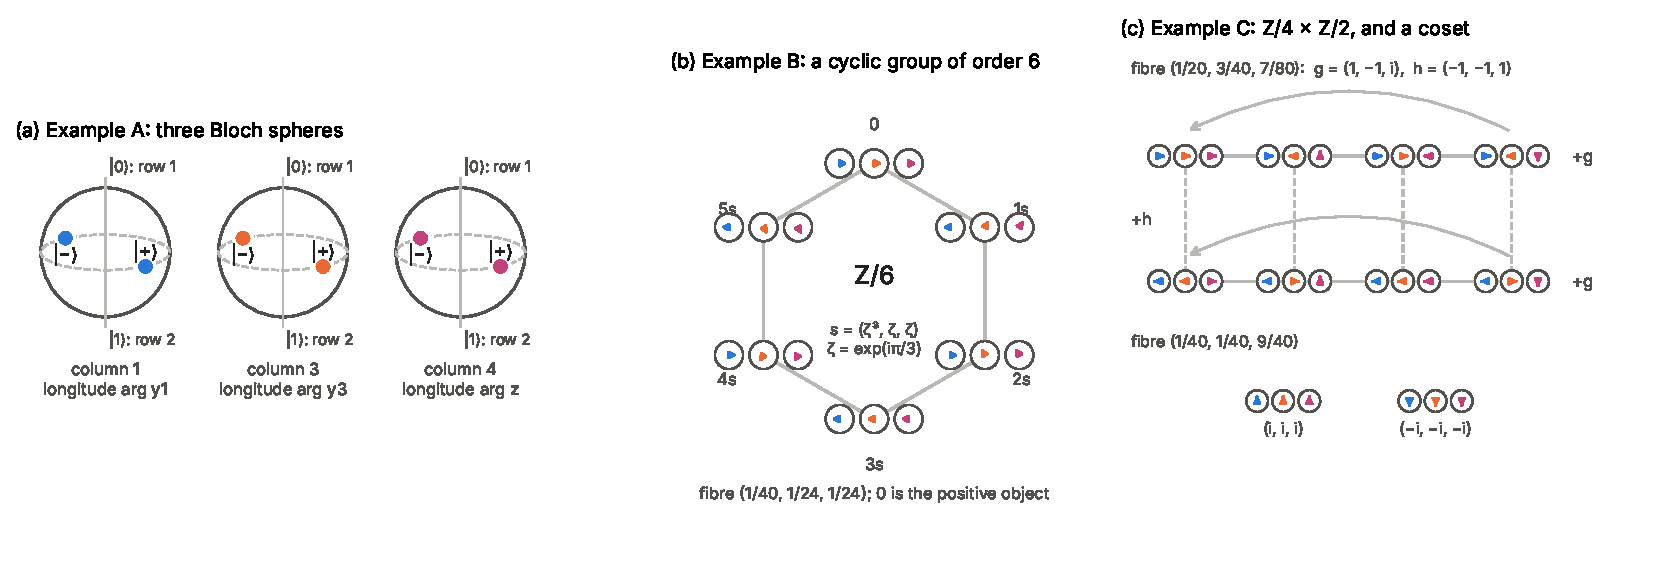
\includegraphics[width=\linewidth]{fig_bloch.pdf}
\caption{Phases of the objects of \cref{fig:tfobjects}. (a) Example A is $(\mathbb{CP}^1)^3$, with one Bloch sphere for each binding column. The height is $P(\text{row }2\mid\text{column})$, which is $1/2$ at the leximin fibre, and the longitude is the holonomy, so the eight objects are the product basis $|{\pm}{\pm}{\pm}\rangle$. (b) B's six holonomies form a cyclic group of order $6$ (dials as in \cref{fig:tfobjects}; each edge adds the generator). (c) C's eight holonomies over the leximin fibre form $\mathbb Z/4\times\mathbb Z/2$, and the two over the other fibre are $\pm(i,i,i)$, which differ by turning all three dials through $\pi$.}\label{fig:bloch}
\end{figure}

\section{Outlook}\label{sec:outlook}
Eight questions are left open.
\begin{itemize}
\item \emph{Novikov weights and environments.} \Cref{sec:data} makes one direction precise: soft evidence of size $n$ on the scale $N$ shifts $\lambda$ by $-(n/N)\rho$.
  Whether the environment orders $s^{r_e}$ of the layers paper act in the same way, and how hard evidence and forgetting act, is open.
\item \emph{The other walls.} Decision, contextuality and value-of-information walls (\cref{sec:data}), and the finite-$n$ sharpness of the transition at an outcome wall,
  measured in the Fisher metric.
\item \emph{Beyond Fano.} For non-Fano toric manifolds, $W$ acquires corrections \cite{FOOO2010}. \Cref{thm:bridge} is about the leading potential only. In the weak Fano chambers of
  $2\times4$ the corrections only rescale coefficients (\cref{rem:corrections}); computing the $\delta_k$, and so the corrected objects of example C, is open.
\item \emph{Composition by selection.} By \cref{prop:nogo}, higher structure with invariant content needs morphism spaces that are not contractible; the natural candidate is the directed
  category of the critical points of $W$, whose Stokes data \cref{sec:path} began to compute \cite{Seidel2008}. On the probabilistic side: continuity of selection across facet-set changes, a
  classification of the associativity locus for binary chains, and $K_5$.
\item \emph{One scale per removed dimension.} \Cref{conj:leveldrop} in general; then $3\times3$, where the fibre is four-dimensional, as a test of it and of the rank equality in \cref{thm:reduction}.
\item \emph{Signed branches and Stokes data.} The non-positive critical points have their own thimbles, which are not real and carry no
  probability law. \Cref{prop:stokes} locates the Stokes walls on $F_1$; the Picard--Lefschetz decomposition itself, and the general window, are not computed. We do not
  know whether the signed fibre of \cref{ex:F1}(a) has a probabilistic shadow. \Cref{sec:path} crosses two leximin walls from the column-binding example; what the collision at the level-two wall does to the category, and an $A_\infty$ functor along a path that avoids it in complexified parameters, are open.
\item \emph{The integral category.} \Cref{thm:shadow} sees the outcome wall in the reduction mod $T$ of one endomorphism algebra. Whether the full $A_\infty$ category over $\Lambda_0$ changes there,
  and split generation in the non-monotone case \cite{Smith2018}, are open.
\item \emph{Wall-crossing.} The layers paper resolves degenerate directions by blow-ups off the torus orbits. Whether these correspond to
  wall-crossing in torus fibrations is a separate question, which needs geometric data that the finite setting does not supply.
\end{itemize}

\appendix
\section{The ledger}\label{app:ledger}
\texttt{LEDGER.yaml} at the root of the repository is the single source for this table, which \texttt{kahler/render\_ledger.py} generates. Status tags: [P] proved
here, [U] used (classical), [C] cited and not proved, [E] exact computation, [N] numerical only, [D] a definition, [O] open. The category level is never
filled by assumption. It records mathematical status, not novelty: [P] there marks a proved standard construction and says so, as for \cref{thm:sec2cat}. For each experiment the ledger also records the thresholds $s_{\mathrm{prob}},s_{\mathrm{support}},s_{\mathrm{trop}},s_{\mathrm{crit}},s_{\mathrm{Stokes}},s_{\mathrm{context}}$, each as a number, ``never'' or ``undefined''. For $F_1$ along $\rho=e_1$
from $\alpha=1/5$ they are: $s_{\mathrm{trop}}=1/5$; $s_{\mathrm{crit}}$ never; $s_{\mathrm{support}}$ never; $s_{\mathrm{prob}}$, $s_{\mathrm{Stokes}}$ and $s_{\mathrm{context}}$ undefined until a dominance notion, a phase of $\hbar$, and a complex
with an obstruction class are chosen.
% generated by kahler/render_ledger.py from LEDGER.yaml; do not edit
{\scriptsize\setlength{\tabcolsep}{3pt}
\begin{longtable}{*{5}{>{\raggedright\arraybackslash}p{0.177\linewidth}}}\toprule
operation & contingency / toric & mirror ($W$, $\lambda$) & Floer (cited); category & wall certificate; checks\\\midrule\endhead
\textbf{soft-translation}: Soft evidence along a translation, rho\_k = $\langle$v\_k, t$\rangle$ (an exponential tilt) & [D] reweighting by a log-linear factor: a reparametrisation of the same model; [P] Q translated by -s t; same Kahler class & [P] u* $\to$ u* - s t; h*, leading set and candidates unchanged & [C] the same fibres, translated; category [O] not addressed & none: rho is orthogonal to B - B (Corollary 12(2)); \textsc{checks} DW7\\
\textbf{soft-constant}: Soft evidence along the constant, rho = 1 (normalisation) & [D] a common factor: removed by normalisation; [P] every facet moves out by s & [P] h* $\to$ h* + s; nothing else changes & [C] no change in which fibres carry Floer cohomology; category [O] not addressed & none: sum\_k a\_k = 0 for every affine dependence a; \textsc{checks} DW7\\
\textbf{soft-circuit}: Soft evidence with a circuit component (lam\_eff = lam - (n/N) rho) & [E] independence: a larger row or column survey (L1 = n1, L2 = n2); 2x3 needs n/2 more column observations to reach its wall; [P] moves the Kahler class; viability walls are the walls of the Kahler cone (F\_1: alpha/L in {0, 1}) & [P] outcome walls = normal fan of the balance polytope B; leading set, candidate dimension and face F jump there; h* concave piecewise linear & [C] F\_1: two fibres with HF $\ne$ 0 below alpha/L = 1/3, one above (Cho-Oh); independence: one fibre on both sides; category [O] no categorical wall-crossing claimed & one circuit a: s* = -c(lam\_0) / $\langle$a, rho$\rangle$; least s over rate range $\le$ 1 is $\vert$c$\vert$ / ($\vert$$\vert$a$\vert$$\vert$\_1 / 2). F\_1: a = (2,-1,2,-3), c = 3 alpha - L; independence: a = (c 1\_r, -r 1\_c)/gcd, c(lam) = (c L1 - r L2)/gcd; \textsc{checks} DW2, DW4, DW5, DW6, DW7, CT2, CT6\\
\textbf{margins}: Observed counts (margins b) & [U] the MLE has the observed margins (Birch); independence: rows x cols / n\^{}2; [U] the fibre over b; l\_k(b) is the k-th margin (independence: exact) & [P] u* does not depend on b while lam is fixed & [D] compare L(b) with the Floer-selected L(u*), in Fisher-Rao distance within the model; category [O] not addressed & support: min\_k l\_k(b) = 0; centrality g(b)/h* = smallest margin / (n / max(r, c)) for independence with joint sampling; \textsc{checks} CT4, CT5\\
\textbf{margins-on-the-fibre}: Margins (f, g) read on the fibre, the coupling polytope Cpl(f, g) & [E] the fibre's lattice points are the tables with these margins; Tier A is Fisher's noncentral hypergeometric family, odds ratios 1 at f(x)g; [U] Cpl(f, g) is Delzant; class = product coupling; 2x3: CP\^{}2, CP\^{}1 x CP\^{}1, F\_1, Bl\_2 CP\^{}2, dP\_6 (coupling-polytopes paper) & [P] h* = min(f\_i/m, g\_j/n); leading cells = the binding row or column; candidate dimension (n-2)(m-1) or (n-1)(m-2) & [C] example: three fibres with HF $\ne$ 0; one count moved: three become two (valuations by exact resultants); category [O] not addressed & the argmin of {f\_i/m, g\_j/n} changes. Example: f1/3 = 2/15 vs g3/2 = 27/200 (1/600 apart): one count crosses; the blow-up wall f1 = g2 is three counts away; \textsc{checks} CF1, CF2, CF3, CF4, CF5, CF6, CF7, CF8\\
\textbf{refinement}: Refinement: add a distinction (a facet normal, a toric blow-up) & [O] which table operation adds a facet is not yet identified; [U] CP\^{}2 $\to$ F\_1 is the blow-up at a point & [E] creates the circuit (2,-1,2,-3) and the wall alpha/L = 1/3; CP\^{}2 had none & [C] F\_1 gains a second fibre with HF $\ne$ 0 below the wall; category [O] not addressed & m - n - 1 increases by one; \textsc{checks} DW4\\
\textbf{structural-zero}: Hard evidence: a structural zero (support restriction) & [E] 2x2 with one structural zero: quasi-independence on three cells; [E] the unit square becomes a unimodular triangle, not a face of it: CP\^{}1 x CP\^{}1 is replaced by CP\^{}2 & [E] the one circuit and the one wall disappear & [C] CP\^{}2: one fibre (the Clifford torus); category [O] not addressed & face test fails; DW circuits of the triangle: none; \textsc{checks} CT7\\
\textbf{independent-product}: Independent product of two models & [E] independence of rows and columns: Delta\_(r-1) x Delta\_(c-1); [U] the product manifold & [P] adds exactly one circuit, the relative scale (q1, -q2); u* = (u1*, u2*) never moves & [C] independence: exactly one fibre with HF $\ne$ 0 for every L1, L2, so this wall changes no Floer data; category [O] Kunneth-type statements not addressed & m - n - 1 = (m1 - n1 - 1) + (m2 - n2 - 1) + 1; \textsc{checks} CT1, CT2, CT3\\
\textbf{forgetting}: Forgetting an environment / marginalisation & [P] the layers paper: the forgetting square, reversal walls, pooled orders; [O] the image configuration under a linear map of exponents: not yet worked out & [O] not yet worked out & [O] not addressed; category [O] not addressed & layers paper, theorem ''contextual Bayes with an environment''; \textsc{checks} EN1, EN2, EN3\\
\textbf{coupling}: Dependent coupling, convolution, intervention, Markov evolution & [O] not yet worked out; [O] convolution would be a Minkowski sum of supports & [O] not yet worked out & [O] not addressed; category [O] not addressed & -; \textsc{checks} --\\
\bottomrule\end{longtable}}


\section{Exact inputs}\label{app:inputs}
Every example can be rebuilt from these data; the checks named in each statement recompute everything else.
\begin{itemize}
\item \emph{The column-binding example and its path} (\cref{sec:cbclass,sec:path}): $f=(2/5,3/5)$, $g=(7/10-\gamma,\,3/10,\,\gamma)$; the example is $\gamma=1/5$, the path $\gamma\in[3/20,11/40]$.
\item \emph{The $2\times4$ examples} (\cref{sec:twofour}): A: $f=(2/5,3/5)$, $g=(1/20,13/20,1/10,1/5)$; B: $f=(3/20,17/20)$, $g=(1/20,1/5,1/4,1/2)$; C: $f=(3/10,7/10)$, $g=(1/10,3/20,1/4,1/2)$. The $148$
chambers are in \texttt{kahler/chambers24.json}.
\item \emph{The binary chain of \cref{thm:k4}}: $\gamma_i=\left(\begin{smallmatrix}t_i&p_i-t_i\\ p_{i+1}-t_i&1-p_i-p_{i+1}+t_i\end{smallmatrix}\right)$ with $(p_0,\dots,p_4)=(2/5,1/3,3/7,1/4,5/11)$ (first entries) and
$(t_1,\dots,t_4)=(13/60,7/30,1/80,3/80)$. The $K_3$ example of \cref{sec:selcomp} is $\gamma_1,\gamma_2,\gamma_3$. \Cref{ex:umbrella} and \cref{sec:howlittle} use $\gamma_1,\gamma_2$, with threshold $\tau=1/2$ on $P(X_2=0\mid X_0=0)$; the other inputs of \cref{prop:selbreaks} are listed there.
\item \emph{The chain with ternary intermediates} (\cref{fig:asconfig}), rows indexed by the first variable:
\[
\gamma_1=\begin{pmatrix}\frac1{150}&\frac{19}{150}&\frac4{15}\\[1pt] \frac4{25}&\frac{31}{150}&\frac7{30}\end{pmatrix},\quad
\gamma_2=\begin{pmatrix}\frac7{50}&\frac2{75}\\[1pt] \frac{18}{175}&\frac{121}{525}\\[1pt] \frac{13}{70}&\frac{11}{35}\end{pmatrix},
\]
\[
\gamma_3=\begin{pmatrix}\frac3{35}&\frac{81}{1400}&\frac{57}{200}\\[1pt] \frac4{35}&\frac{339}{1400}&\frac{43}{200}\end{pmatrix},\quad
\gamma_4=\begin{pmatrix}\frac9{125}&\frac{23}{375}&\frac1{15}\\[1pt] \frac{209}{3000}&\frac{79}{750}&\frac18\\[1pt] \frac{13}{120}&\frac16&\frac9{40}\end{pmatrix}.
\]
\item \emph{The cells of associativity} (\cref{prop:assoclocus}(2)): margins $(2/5,1/3,3/7,1/4)$ at the point $(13/60,7/30,29/240)$, and margins $(3/20,1/4,3/4,17/20)$ at the point
$(1/40,1/48,51/80)$. The check SX1 prints the inequalities of both cells.
\end{itemize}

\section*{Checks}
\begin{center}\small
\begin{tabular}{ll}\toprule
code & \texttt{engine/pce/kahlerbridge.py}, \texttt{engine/pce/datawalls.py},\\ & \texttt{engine/pce/contingency\_toric.py}, \texttt{engine/pce/couplingfibre.py},\\ & \texttt{engine/pce/floermorph.py}, \texttt{engine/pce/colbind.py},\\ & \texttt{engine/pce/cpl24.py}, \texttt{engine/pce/pentpath.py},\\ & \texttt{engine/pce/selcomp.py}\\
checks & \texttt{engine/check\_kahlerbridge.py} (KB, $8/8$), \texttt{engine/check\_datawalls.py} (DW, $7/7$),\\
 & \texttt{engine/check\_contingency\_toric.py} (CT, $7/7$),\\ & \texttt{engine/check\_couplingfibre.py} (CF, $8/8$), \texttt{engine/check\_leximin.py} (LX, $9/9$),\\ & \texttt{engine/check\_floermorph.py} (MO, $9/9$), \texttt{engine/check\_colbind.py} (CB, $8/8$),\\ & \texttt{engine/check\_cpl24.py} (TF, $9/9$), \texttt{engine/check\_pentpath.py} (PP, $9/9$),\\ & \texttt{engine/check\_selcomp.py} (AS, $7/7$), \texttt{engine/check\_selbin.py} (SB, $7/7$),\\ & \texttt{engine/check\_selcert.py} (SX, $3/3$), \texttt{engine/check\_selfloer.py} (SF, $5/5$),\\ & \texttt{engine/check\_chambers24\_cert.py} (CC, $4/4$), \texttt{engine/check\_ledger.py} (LG, $3/3$)\\
figures & \texttt{kahler/fig\_kahler.py}, \texttt{kahler/fig\_datawalls.py}, \texttt{kahler/fig\_coupling.py},\\ & \texttt{kahler/fig\_leximin.py}, \texttt{kahler/fig\_morph.py}, \texttt{kahler/fig\_colbind.py},\\ & \texttt{kahler/fig\_cpl24.py}, \texttt{kahler/fig\_pentpath.py},\\ & \texttt{kahler/fig\_selcomp.py}, \texttt{kahler/fig\_selbin.py}\\ certificate & \texttt{kahler/chambers24.json}\\ ledger & \texttt{LEDGER.yaml}, rendered by \texttt{kahler/render\_ledger.py}\\\bottomrule
\end{tabular}
\end{center}
The checks corroborate the statements numerically, or by exact rational arithmetic where marked; they do not prove them.
The proofs stand on their own. The $F_1$ blow-up sizes used are $\alpha=1/5,\,1/4,\,2/5,\,3/5,\,4/5$.
{\small
\begin{longtable}{lp{0.82\linewidth}}\toprule
KB1 & \cref{prop:kahler}(1)--(2): moment map $=\nabla\varphi$, Fisher information $=\operatorname{Hess}\varphi$, positive definite ($30$ supports)\\
KB2 & \cref{prop:kahler}(4): $\psi=\sum q\log(q/c)$, $\nabla\psi=u(p)$, $\operatorname{Hess}\psi=$ Fisher$^{-1}$ ($20$ supports)\\
KB3 & \cref{prop:kahler}(5): $\int\det\operatorname{Hess}\varphi$ over boxes equals the area of the moment image\\
KB4 & \cref{thm:bridge}(1)--(2): one positive critical point, mean-zero law, the valuations of \cref{ex:CP2,ex:F1}, balanced leading terms\\
KB5 & \cref{thm:bridge}(3): the segment of candidates for $\alpha=3/5$, and its endpoints $(1/5,1/5)$, $(3/5,1/5)$, with leading sets $\{v_1,v_2,v_4\}$, $\{v_2,v_3,v_4\}$ and no positive balance; the barycentre alone for $\alpha=1/5$ and for $\mathbb{CP}^2$ (exact rational points)\\
KB6 & \cref{thm:bridge}(4): all four critical points of $F_1$ in $80$-digit arithmetic; the signed critical point and its signed balance\\
KB7 & \cref{prop:thimble}: Hessian $\operatorname{diag}(H,-H)$ at $y_T$; Laplace covariance $\hbar H^{-1}$ with relative error $O(\hbar/W_T(y_T))$ ($\mathbb{CP}^2$, $F_1$ with $\alpha=3/5$)\\
KB8 & \cref{thm:tropical}, \cref{ex:levels}: moments against the uniform law on $Q_h$ for $h<h^*$; concentration on $\operatorname{argmax}g$ at $h^*$; the uniform segment; the levels $3/10$, $9/20$; $\log T=-200,-800$\\
DW1 & \cref{conv:data}: evidence $e^{-n\rho}$ at $T=e^{-N}$ is the shift $\lambda-(n/N)\rho$\\
DW2 & \cref{prop:balancelp}(1)--(2): duality; optimal support $=$ leading set at the centre of $\operatorname{argmax}$; $\dim\operatorname{argmax}=n-\dim\sigma_0$ ($40$ random configurations)\\
DW3 & \cref{prop:balancelp}(3): the limit law lies in the optimal face ($23$ cases)\\
DW4 & \cref{ex:F1wall}(a): the circuit $(2,-1,2,-3)$; the wall $\alpha/L=1/3$ inside $0<\alpha/L<1$; the diagonal flip (exact rationals); $\mathbb{CP}^2$ one chamber\\
DW5 & \cref{ex:F1wall}(b),(c): candidates and valuations for $\alpha=1/10,\dots,9/10$; the wall law from $x^4=x+1$ at $T=10^{-20},10^{-60}$\\
DW6 & \cref{ex:F1wall}(d): the discriminant, symbolically; its terms tie only at $\alpha=1/3$\\
DW7 & \cref{cor:where}, \cref{ex:F1wall}(e): $s^*=1/5$ for $\rho=e_1$; no wall for $e_4$, $(0,-1,0,1)$, translations or constants; least evidence $1/10$; $\mathbb{CP}^2$ never\\
CT1 & \cref{prop:twoconf}: $(r-1)(c-1)$ moves; one facet circuit ($r,c\in\{2,3,4\}$)\\
CT2 & \cref{thm:indep}(1): $h^*$, the leading sets and the wall $cL_1=rL_2$ (exact rationals)\\
CT3 & \cref{thm:indep}(2)--(3): the $rc$ critical points and their common valuation; the exact positive law; candidate dimensions\\
CT4 & \cref{prop:roles}(1): $\ell_k(b)=$ margins; MLE margins and positivity ($200$ tables)\\
CT5 & \cref{prop:roles}(3): the block-diagonal Fisher information; properties of $d_\Delta$\\
CT6 & \cref{ex:2x3}: $h^*=n/3$, the candidate segment, $u^*$, and $n/2$ more column observations\\
CT7 & \cref{ex:zero}: the triangle is not a face; no circuit\\
CF1--CF2 & \cref{ex:pentagon}: the pentagon, its facets, Delzant; $715$ tables (Pick), exact\\
CF3 & \cref{prop:hypergeom}: odds-ratio identity; exact hypergeometric mean $(12,86/5)$; Birch at the leximin\\
CF4 & \cref{thm:maxmincoupling}(1)--(3): the closed form against the facet programme; binding cells are facets; candidate dimensions\\
CF5 & \cref{ex:fivecrit}: five critical points by exact resultants; positions, signs, leading sets, signed balances\\
CF6 & \cref{thm:maxmincoupling}(4): positive valuation $=$ leximin coupling ($20$ random margins)\\
CF7 & \cref{fig:cplthimble}: the thimble law against uniform on $Q_h$; concentration at the leximin\\
CF8 & \cref{ex:onecount}: one count; the walls' distances; three valuations become two\\
LX1--LX3 & \cref{thm:selection}: $L|u_L-u^{\mathrm{lex}}|$ bounded on $30$ random configurations (multiprecision Newton); the projected equation; $\mathbb{CP}^2$, $F_1$\\
LX4 & \cref{cor:leximin}: facet-leximin $=$ all-cell leximin ($292$ margins); convergence\\
LX5--LX9 & \cref{ex:colbind}: the fibre and its two levels (exact); the $\ln2/2$ correction; the five critical points; the thimble; the one-count levels\\
MO1--MO2 & the objects of $F_1$ and of the $2\times3$ fibres: counts, fibres, types, holonomies\\
MO3--MO5 & \cref{prop:morph}: disjoint fibres, distinct holonomies and values; $Q=W\operatorname{Cov}_w(v)$; Clifford generators spanning $M_2$ ($18$ objects)\\
MO6 & \cref{thm:shadow}: $Q/W\to\operatorname{Cov}_{q^*}(v)$; reduced ranks $2,2,1,1$ on $F_1$; $2\to1$ after one count; valuations of the small eigenvalue\\
MO7 & \cref{thm:compare}: no collision, Morse along $\alpha\in[1/5,3/5]$; explicit real isomorphisms\\
MO8--MO9 & \cref{prop:stokes}: Stokes walls within $4/\log(1/T)$ of the wall, none outside, rate $1/\log(1/T)$\\
CB1--CB4 & \cref{prop:five}: the reduction to the quintic; the Newton polygon; distinct and nondegenerate for all $T>0$; distinct critical values on $(0,1)$ (exact, symbolic)\\
CB5--CB6 & the table of \cref{sec:cbclass}: leading coefficients, offsets $-\log|\rho|/L$, leading values; leading Clifford forms and determinants\\
CB7 & \cref{prop:homtable}: $5$ objects, $2$ fibres; distinct values and holonomies; $\mathrm{Cl}(Q_c)\cong M_2$\\
CB8 & \cref{thm:reduction}: (H1), convergence to $M_c$, rank $=$ span on $23$ objects\\
PP1--PP2 & \cref{prop:path}(1): one K\"ahler chamber along the path; the leximin levels and the two walls (exact)\\
PP3--PP4 & \cref{prop:path}(2)--(3): the reduction to \eqref{eq:pathquintic}; Newton polygons at $10$ rational $\gamma$ (exact)\\
PP5 & \cref{prop:path}(3): valuations, real and complex types, leading phases at $L=200,400$\\
PP6 & \cref{prop:crossing}(1)--(2): one discriminant zero, at the level-two wall, for $L=50,\dots,400$; none at the level-one wall\\
PP7 & \cref{prop:crossing}(3): no coincidence of critical values away from the collision\\
PP8 & \cref{prop:crossing}(4): the positive object's scale against $h_2-h_1$ along the path\\
PP9 & Stokes alignments at three phases and three $L$, within $1.5/L$ of a wall\\
TF1 & \cref{thm:chambers24}: $148$ chambers, each with an exact interior point; all simple and smooth\\
TF2 & \cref{prop:kleiman}(3): integer wall relations on all $2208$ edges; the K\"ahler degree equals the lattice length (exact)\\
TF3 & \cref{thm:chambers24}: the six types by toric Kleiman; the vertex test agrees; volume $=\chi$; $(-K)^3=64,56,48,48,40,32$\\
TF4 & \cref{prop:fanodepth}: the box criterion on all chambers; the facets of the $\mathbb{CP}^3$ and $\mathrm{Bl}_{pt}\mathbb{CP}^3$ chambers\\
TF5 & \cref{ex:A24}: $8$ critical points over one fibre; the one coincidence of critical values at $x^3+x-1=0$ (exact)\\
TF6 & \cref{prop:B24}(2)--(4): the sextic, its discriminants, one fibre, holonomies $(\zeta^{-3},\zeta,\zeta)$ (exact)\\
TF7 & \cref{ex:C24}: degree-$10$ resultant, its Newton polygon, $8+2$ critical points over two fibres; three curves with $-K\cdot C=0$\\
TF8 & \cref{prop:fanodepth,ex:A24,prop:B24,ex:C24}: the leximin levels and drops exactly; a tie-free census of drop patterns by chamber type\\
TF9 & \cref{prop:scales}: eigenvalue slopes at the positive object ($L=800\to1600$); minors on all $22$ leximin-fibre objects; rank $3$ on C's second fibre\\
CC1--CC4 & \cref{thm:chambers24}: the certificate \texttt{kahler/chambers24.json}, verified independently (standard library, exact rationals)\\
AS1--AS2 & \cref{prop:markovglue}: Markov gluing associative and unital, one composite per face, maximal entropy (exact); face counts of $K_3,K_4,K_5$\\
AS3--AS4 & \cref{thm:k4}: the eleven composites, binary and with ternary intermediates (exact rationals)\\
AS5--AS6 & \cref{prop:selprops}: unit and transposition (exact); the non-associativity census\\
AS7 & finite $T$: the associator $-41/960$ at every $L$; convergence of the composites\\
SB1--SB2 & \cref{thm:frechet,cor:tropcorr}: Fr\'echet-midpoint gluing on $60$ chains; signed-minimum correlations and associativity on uniform margins (exact)\\
SB3--SB4 & continuity: affine on a fixed type (exact); no jump across $\ge10$ facet-set changes (numerical)\\
SB5--SB6 & \cref{prop:assoclocus}: only uniform margins associative among $9^4$ tuples; the locus has positive measure (exact grids)\\
SB7 & \cref{ex:assoc1}: the one-parameter associator, its kinks and zeros (exact)\\
SX1 & \cref{prop:assoclocus}(2): two full-dimensional cells where $A=0$ (exact)\\
SX2 & \cref{thm:k4} and the ternary example: exact certificates for all $57$ selections\\
SX3 & the ternary configuration: hull, Markov point and crossings by exact orientation tests\\
SF1--SF3 & \cref{prop:selfloer}: the fibre is $\prod\mathbb{CP}^1$ (exact traversal); Cho--Oh and Alston--Amorim conditions at the midpoints (exact)\\
SF4--SF5 & Birch against Floer points; the $K_4$ fibres: Delzant, orbifold and Fano tests (exact traversal)\\
NC1--NC3 & \cref{prop:cplcat,prop:selkeeps}: the dagger symmetric monoidal structure of Markov gluing; units, reversal, relabelling and copied factors for selection (exact)\\
NC4--NC6 & \cref{prop:selbreaks}: the tensor, end and middle counterexamples, with all inputs (exact)\\
NC7 & \cref{prop:identified}: the identified interval against linear programs over the fibre; selection at its centre\\
NC8--NC9 & \cref{ex:howlittle}: the interval, worst-case errors, flipping edits and zero-cost changes (exact)\\
MS1--MS2 & \cref{thm:sections,thm:sec2cat}: both rules are sections, equivariant; maximum entropy is the inner-face consistent Markov chain, leximin is not\\
MS3--MS5 & \cref{prop:cycleD,prop:cyclefibres}: the 24 facets of $\mathcal D$; the 2721 faces and their fibre dimensions; contextual data on the symmetric path (exact)\\
MS6--MS7 & \cref{prop:chshpath} and the path table: symmetric path (exact rank; interval numerical); generic paths (numerical)\\
MS8--MS9 & \cref{prop:simpson}: the two Simpson reversals (exact)\\
MS10 & \cref{thm:ncycle}: all facets of $\mathcal D$ for the $n$-cycle, $n=3,4,5$; the listed facets and vertex counts for $n=6,7,8$ (exact)\\
MS11 & \cref{prop:cocycle}: the $c<0$ example (exact); the tensor-square defect along the power family (numerical)\\
LG1--LG3 & \cref{app:ledger}: the schema; every cited check passes in the log; the rendered table matches \texttt{LEDGER.yaml}\\\bottomrule
\end{longtable}}

\section*{Acknowledgement}
Much of the text, the code, the check scripts and the figures were drafted with an AI system (Claude, Anthropic), as stated after the abstract. Some review comments used in the revisions were also generated with AI tools. The author directed the work, proposed its questions, including the comparison with Bloch spheres and pseudo-knots, checked the statements against the computations recorded in the ledger, and takes responsibility for the content.

\begin{thebibliography}{99}
\bibitem{AbramskyBarbosaMansfield2017} S.~Abramsky, R.~Soares Barbosa and S.~Mansfield, Contextual fraction as a measure of contextuality, \emph{Phys. Rev. Lett.} \textbf{119} (2017) 050504.
\bibitem{AbramskyBrandenburger2011} S.~Abramsky and A.~Brandenburger, The sheaf-theoretic structure of non-locality and contextuality, \emph{New J. Phys.} \textbf{13} (2011) 113036.
\bibitem{AbramskyMansfieldBarbosa2012} S.~Abramsky, S.~Mansfield and R.~Soares Barbosa, The cohomology of non-locality and contextuality, \emph{Electron. Proc. Theor. Comput. Sci.} \textbf{95} (2012) 1--14.
\bibitem{Abreu2003} M.~Abreu, K\"ahler geometry of toric manifolds in symplectic coordinates, in \emph{Symplectic and Contact Topology}, Fields Inst. Commun. \textbf{35}, AMS, 2003, 1--24.
\bibitem{Aubin1991} J.-P.~Aubin, \emph{Viability Theory}, Birkh\"auser, 1991.
\bibitem{AlSafiShort2013} S.~W.~Al-Safi and A.~J.~Short, Simulating all nonsignaling correlations via classical or quantum theory with negative probabilities, \emph{Phys. Rev. Lett.} \textbf{111} (2013) 170403.
\bibitem{AmariNagaoka2000} S.~Amari and H.~Nagaoka, \emph{Methods of Information Geometry}, AMS and Oxford University Press, 2000.
\bibitem{AlstonAmorim2010} G.~Alston and L.~Amorim, Floer cohomology of torus fibers and real Lagrangians in Fano toric manifolds, arXiv:1003.3651, 2010.
\bibitem{AraujoEtAl2013} M.~Ara\'ujo, M.~T.~Quintino, C.~Budroni, M.~Terra Cunha and A.~Cabello, All noncontextuality inequalities for the $n$-cycle scenario, \emph{Phys. Rev. A} \textbf{88} (2013) 022118.
\bibitem{Auroux2007} D.~Auroux, Mirror symmetry and T-duality in the complement of an anticanonical divisor, \emph{J. G\"okova Geom. Topol.} \textbf{1} (2007) 51--91.
\bibitem{Awasthi2026Br} V.~K.~Awasthi, Bridges: from probability and entropy to branes, with worked examples, technical note, Johns Hopkins University, October 2026.
\bibitem{Awasthi2026Cpl} V.~K.~Awasthi, Coupling polytopes and toric geometry: the $2\times3$ family, the square case, higher levels and stability, companion paper, Johns Hopkins University, October 2026.
\bibitem{Awasthi2026Arch} V.~K.~Awasthi, How the programme fits together: one family of polytopes, many models, and one example through every layer, draft 1, Johns Hopkins University, October 2026.
\bibitem{BaudotBennequin2015} P.~Baudot and D.~Bennequin, The homological nature of entropy, \emph{Entropy} \textbf{17} (2015) 3253--3318.
\bibitem{BeckRobins2015} M.~Beck and S.~Robins, \emph{Computing the Continuous Discretely}, 2nd ed., Springer, 2015.
\bibitem{BilleraSturmfels1992} L.~J.~Billera and B.~Sturmfels, Fiber polytopes, \emph{Ann. of Math.} \textbf{135} (1992) 527--549.
\bibitem{ClauserHorne1974} J.~F.~Clauser and M.~A.~Horne, Experimental consequences of objective local theories, \emph{Phys. Rev. D} \textbf{10} (1974) 526--535.
\bibitem{CressieRead1984} N.~Cressie and T.~R.~C.~Read, Multinomial goodness-of-fit tests, \emph{J. Roy. Statist. Soc. Ser. B} \textbf{46} (1984) 440--464.
\bibitem{Csiszar1975} I.~Csisz\'ar, $I$-divergence geometry of probability distributions and minimization problems, \emph{Ann. Probab.} \textbf{3} (1975) 146--158.
\bibitem{Das2023} N.~Das, Credal imprecision and the value of evidence, \emph{No\^us} 57 (2023) 684--721; doi:10.1111/nous.12417.
\bibitem{Hanaki2010} R.~Hanaki, Pseudo diagrams of knots, links and spatial graphs, \emph{Osaka J. Math.} \textbf{47} (2010) 863--883.
\bibitem{Lauritzen1996} S.~L.~Lauritzen, \emph{Graphical Models}, Oxford University Press, 1996.
\bibitem{Nerode1958} A.~Nerode, Linear automaton transformations, \emph{Proc.\ Amer.\ Math.\ Soc.} \textbf{9} (1958) 541--544.
\bibitem{Conway1970} J.~H.~Conway, An enumeration of knots and links, and some of their algebraic properties, in \emph{Computational Problems in Abstract Algebra}, Pergamon, 1970, 329--358.
\bibitem{Fliess1974} M.~Fliess, Matrices de Hankel, \emph{J.\ Math.\ Pures Appl.} \textbf{53} (1974) 197--224.
\bibitem{CoxLittleOShea2015} D.~A.~Cox, J.~Little and D.~O'Shea, \emph{Ideals, Varieties, and Algorithms}, 4th ed., Springer, 2015.
\bibitem{BokutChen2014} L.~A.~Bokut and Y.~Chen, Gr\"obner--Shirshov bases and their calculation, \emph{Bull.\ Math.\ Sci.} \textbf{4} (2014) 325--395.
\bibitem{Bokut2008} L.~A.~Bokut, Gr\"obner--Shirshov basis for the braid group in the Birman--Ko--Lee--Garside generators, arXiv:0806.1123 (2008).
\bibitem{CransHenrichNelson2013} A.~S.~Crans, A.~Henrich and S.~Nelson, Polynomial knot and link invariants from the virtual biquandle, \emph{J.\ Knot Theory Ramifications} \textbf{22}(4) (2013); arXiv:1110.1371.
\bibitem{NosakaShimizu2026} T.~Nosaka and K.~Shimizu, Gr\"obner bases for Alexander Fitting ideals of links, arXiv:2608.25725 (2026).
\bibitem{Reiter1987} R.~Reiter, A theory of diagnosis from first principles, \emph{Artificial Intelligence} \textbf{32} (1987) 57--95.
\bibitem{Rubin1976} D.~B.~Rubin, Inference and missing data, \emph{Biometrika} \textbf{63} (1976) 581--592.
\bibitem{CartierFoata1969} P.~Cartier and D.~Foata, \emph{Probl\`emes combinatoires de commutation et r\'earrangements}, Lecture Notes in Mathematics 85, Springer, 1969.
\bibitem{DiekertRozenberg1995} V.~Diekert and G.~Rozenberg (eds.), \emph{The Book of Traces}, World Scientific, 1995.
\bibitem{Artin1947} E.~Artin, Theory of braids, \emph{Ann.\ of Math.} \textbf{48} (1947) 101--126.
\bibitem{Rolfsen1976} D.~Rolfsen, \emph{Knots and Links}, Publish or Perish, 1976.
\bibitem{Birman1974} J.~S.~Birman, \emph{Braids, Links, and Mapping Class Groups}, Annals of Mathematics Studies \textbf{82}, Princeton University Press, 1974.
\bibitem{Milnor1954} J.~Milnor, Link groups, \emph{Ann.\ of Math.} \textbf{59} (1954) 177--195.
\bibitem{HabeggerLin1990} N.~Habegger and X.-S.~Lin, The classification of links up to link-homotopy, \emph{J.\ Amer.\ Math.\ Soc.} \textbf{3} (1990) 389--419.
\bibitem{Chen1977} K.-T.~Chen, Iterated path integrals, \emph{Bull.\ Amer.\ Math.\ Soc.} \textbf{83} (1977) 831--879.
\bibitem{Kohno1985} T.~Kohno, S\'erie de Poincar\'e--Koszul associ\'ee aux groupes de tresses pures, \emph{Invent.\ Math.} \textbf{82} (1985) 57--75.
\bibitem{Stone1961} M.~Stone, The opinion pool, \emph{Ann.\ Math.\ Statist.} \textbf{32} (1961) 1339--1342.
\bibitem{GenestZidek1986} C.~Genest and J.~V.~Zidek, Combining probability distributions: a critique and an annotated bibliography, \emph{Statist.\ Sci.} \textbf{1} (1986) 114--148.
\bibitem{GenestMcConwaySchervish1986} C.~Genest, K.~J.~McConway and M.~J.~Schervish, Characterization of externally Bayesian pooling operators, \emph{Ann.\ Statist.} \textbf{14} (1986) 487--501.
\bibitem{Granger1969} C.~W.~J.~Granger, Investigating causal relations by econometric models and cross-spectral methods, \emph{Econometrica} \textbf{37} (1969) 424--438.
\bibitem{Wilson1927} E.~B.~Wilson, Probable inference, the law of succession, and statistical inference, \emph{J.\ Amer.\ Statist.\ Assoc.} \textbf{22} (1927) 209--212.
\bibitem{DuchampKrob1992} G.~Duchamp and D.~Krob, The lower central series of the free partially commutative group, \emph{Semigroup Forum} \textbf{45} (1992) 385--394.
\bibitem{GohmKostler2009} R.~Gohm and C.~K\"ostler, Noncommutative independence from the braid group $\mathbb B_\infty$, \emph{Comm.\ Math.\ Phys.} \textbf{289} (2009) 435--482.
\bibitem{Nechaev1998} S.~Nechaev, Statistics of knots and entangled random walks, lectures at the Les Houches summer school 1998, arXiv:cond-mat/9812205.
\bibitem{Collins1994} D.~J.~Collins, Relations among the squares of the generators of the braid group, \emph{Invent.\ Math.} \textbf{117} (1994) 525--529.
\bibitem{HamblyLyons2010} B.~Hambly and T.~Lyons, Uniqueness for the signature of a path of bounded variation and the reduced path group, \emph{Ann.\ of Math.} \textbf{171} (2010) 109--167.
\bibitem{AbramskyCaru2019} S.~Abramsky and G.~Car\`u, Non-locality, contextuality and valuation algebras: a general theory of disagreement, \emph{Phil.\ Trans.\ R.\ Soc.\ A} \textbf{377} (2019) 20190036.
\bibitem{Iannucci2025} L.~Iannucci, E.~Muratore, A.~Matakos and M.~Kivel\"a, Detecting coordinated activities through temporal, multiplex, and collaborative analysis, arXiv:2512.19677 (2025).
\bibitem{Kauffman1987} L.~H.~Kauffman, State models and the Jones polynomial, \emph{Topology} \textbf{26} (1987) 395--407.
\bibitem{Khovanov2000} M.~Khovanov, A categorification of the Jones polynomial, \emph{Duke Math. J.} \textbf{101} (2000) 359--426.
\bibitem{BarNatan2002} D.~Bar-Natan, On Khovanov's categorification of the Jones polynomial, \emph{Algebr. Geom. Topol.} \textbf{2} (2002) 337--370.
\bibitem{HeuslerSchlummerUbben2020} S.~Heusler, P.~Schlummer and M.~S.~Ubben, A knot theoretic extension of the Bloch sphere representation for qubits in Hilbert space and its application to contextuality and many-worlds theories, \emph{Symmetry} \textbf{12} (2020) 1135.
\bibitem{Mermin1990} N.~D.~Mermin, Simple unified form for the major no-hidden-variables theorems, \emph{Phys. Rev. Lett.} \textbf{65} (1990) 3373--3376.
\bibitem{Peres1990} A.~Peres, Incompatible results of quantum measurements, \emph{Phys. Lett. A} \textbf{151} (1990) 107--108.
\bibitem{DiamantisKauffman2026} I.~Diamantis and L.~H.~Kauffman, Probabilistic pseudo knot theory, arXiv:2607.08188 (2026).
\bibitem{DrtonSturmfelsSullivant2009} M.~Drton, B.~Sturmfels and S.~Sullivant, \emph{Lectures on Algebraic Statistics}, Birkh\"auser, 2009.
\bibitem{Fine1982} A.~Fine, Hidden variables, joint probability, and the Bell inequalities, \emph{Phys. Rev. Lett.} \textbf{48} (1982) 291--295.
\bibitem{Hora2023} R.~Hora, Internal parameterization of hyperconnected quotients, arXiv:2302.06851 (2023).
\bibitem{Layers} V.~K.~Awasthi, Probability, context and differentiation: the layers, working draft, 2026.
\bibitem{Birch1963} M.~W.~Birch, Maximum likelihood in three-way contingency tables, \emph{J. Roy. Statist. Soc. Ser. B} \textbf{25} (1963) 220--233.
\bibitem{BishopFienbergHolland1975} Y.~M.~M.~Bishop, S.~E.~Fienberg and P.~W.~Holland, \emph{Discrete Multivariate Analysis}, MIT Press, 1975.
\bibitem{BochnakCosteRoy1998} J.~Bochnak, M.~Coste and M.-F.~Roy, \emph{Real Algebraic Geometry}, Ergebnisse der Mathematik \textbf{36}, Springer, 1998.
\bibitem{ChoOh2006} C.-H.~Cho and Y.-G.~Oh, Floer cohomology and disc instantons of Lagrangian torus fibers in Fano toric manifolds, \emph{Asian J. Math.} \textbf{10} (2006) 773--814.
\bibitem{Cho2005} C.-H.~Cho, Products of Floer cohomology of torus fibers in toric Fano manifolds, \emph{Comm. Math. Phys.} \textbf{260} (2005) 613--640.
\bibitem{ChoJacobs2019} K.~Cho and B.~Jacobs, Disintegration and Bayesian inversion via string diagrams, \emph{Math. Structures Comput. Sci.} \textbf{29} (2019) 938--971.
\bibitem{CLLT2020} K.~Chan, S.-C.~Lau, N.~C.~Leung and H.-H.~Tseng, Open Gromov--Witten invariants and mirror maps for semi-Fano toric manifolds, \emph{Pure Appl. Math. Q.} \textbf{16} (2020) 675--720.
\bibitem{CLS2011} D.~A.~Cox, J.~B.~Little and H.~K.~Schenck, \emph{Toric Varieties}, Graduate Studies in Mathematics \textbf{124}, American Mathematical Society, 2011.
\bibitem{CominettiSanMartin1994} R.~Cominetti and J.~San Mart\'in, Asymptotic analysis of the exponential penalty trajectory in linear programming, \emph{Math. Programming} \textbf{67} (1994) 169--187.
\bibitem{Delzant1988} T.~Delzant, Hamiltoniens p\'eriodiques et images convexes de l'application moment, \emph{Bull. Soc. Math. France} \textbf{116} (1988) 315--339.
\bibitem{DiaconisZabell1982} P.~Diaconis and S.~L.~Zabell, Updating subjective probability, \emph{J. Amer. Statist. Assoc.} \textbf{77} (1982) 822--830.
\bibitem{DiaconisSturmfels1998} P.~Diaconis and B.~Sturmfels, Algebraic algorithms for sampling from conditional distributions, \emph{Ann. Statist.} \textbf{26} (1998) 363--397.
\bibitem{DuistermaatHeckman1982} J.~J.~Duistermaat and G.~J.~Heckman, On the variation in the cohomology of the symplectic form of the reduced phase space, \emph{Invent. Math.} \textbf{69} (1982) 259--268.
\bibitem{Dyckerhoff2011} T.~Dyckerhoff, Compact generators in categories of matrix factorizations, \emph{Duke Math. J.} \textbf{159} (2011) 223--274.
\bibitem{EFRS2006} N.~Eriksson, S.~E.~Fienberg, A.~Rinaldo and S.~Sullivant, Polyhedral conditions for the nonexistence of the MLE for hierarchical log-linear models, \emph{J. Symbolic Comput.} \textbf{41} (2006) 222--233.
\bibitem{FienbergRinaldo2012} S.~E.~Fienberg and A.~Rinaldo, Maximum likelihood estimation in log-linear models, \emph{Ann. Statist.} \textbf{40} (2012) 996--1023.
\bibitem{Fisher1935} R.~A.~Fisher, The logic of inductive inference, \emph{J. Roy. Statist. Soc.} \textbf{98} (1935) 39--82.
\bibitem{FOOO2010} K.~Fukaya, Y.-G.~Oh, H.~Ohta and K.~Ono, Lagrangian Floer theory on compact toric manifolds I, \emph{Duke Math. J.} \textbf{151} (2010) 23--174.
\bibitem{Fritz2020} T.~Fritz, A synthetic approach to Markov kernels, conditional independence and theorems on sufficient statistics, \emph{Adv. Math.} \textbf{370} (2020) 107239.
\bibitem{Fulton1993} W.~Fulton, \emph{Introduction to Toric Varieties}, Annals of Mathematics Studies \textbf{131}, Princeton University Press, 1993.
\bibitem{Galkin2014} S.~Galkin, The conifold point, arXiv:1404.7388, 2014.
\bibitem{GGI2016} S.~Galkin, V.~Golyshev and H.~Iritani, Gamma classes and quantum cohomology of Fano manifolds: Gamma conjectures, \emph{Duke Math. J.} \textbf{165} (2016) 2005--2077.
\bibitem{GeigerMeekSturmfels2006} D.~Geiger, C.~Meek and B.~Sturmfels, On the toric algebra of graphical models, \emph{Ann. Statist.} \textbf{34} (2006) 1463--1492.
\bibitem{GKZ1994} I.~M.~Gelfand, M.~M.~Kapranov and A.~V.~Zelevinsky, \emph{Discriminants, Resultants, and Multidimensional Determinants}, Birkh\"auser, 1994.
\bibitem{GensbittelPeskiRenault2022} F.~Gensbittel, M.~\Peski{} and J.~Renault, Value-based distance between information structures, \emph{Theoretical Economics} 17 (2022) 1225--1267; doi:10.3982/TE4782.
\bibitem{Guillemin1994} V.~Guillemin, Kaehler structures on toric varieties, \emph{J. Differential Geom.} \textbf{40} (1994) 285--309.
\bibitem{HoriVafa2000} K.~Hori and C.~Vafa, Mirror symmetry, arXiv:hep-th/0002222, 2000.
\bibitem{Iritani2009} H.~Iritani, An integral structure in quantum cohomology and mirror symmetry for toric orbifolds, \emph{Adv. Math.} \textbf{222} (2009) 1016--1079.
\bibitem{JuddRietsch2019} J.~Judd and K.~Rietsch, The tropical critical point and mirror symmetry, arXiv:1911.04463, 2019.
\bibitem{Kleiman1966} S.~L.~Kleiman, Toward a numerical theory of ampleness, \emph{Ann. of Math.} \textbf{84} (1966) 293--344.
\bibitem{Kadeishvili1980} T.~V.~Kadeishvili, On the homology theory of fibre spaces, \emph{Russian Math. Surveys} \textbf{35} (1980) 231--238.
\bibitem{MaclaganSturmfels2015} D.~Maclagan and B.~Sturmfels, \emph{Introduction to Tropical Geometry}, Graduate Studies in Mathematics \textbf{161}, AMS, 2015.
\bibitem{Iskandar2026} R.~Iskandar, Value of information under imprecise probabilities: decision rule-specific values and fixed-measure envelopes on a credal set, arXiv:2607.06570 (2026).
\bibitem{Manski2003} C.~F.~Manski, \emph{Partial Identification of Probability Distributions}, Springer Series in Statistics, Springer, 2003.
\bibitem{BohinenPerrone2025} M.~Bohinen and P.~Perrone, Categorical algebra of conditional probability, \emph{Appl.\ Categ.\ Structures} (2026), doi:10.1007/s10485-026-09893-9; arXiv:2502.14941.
\bibitem{BroderickGiordanoMeager2020} T.~Broderick, R.~Giordano and R.~Meager, An automatic finite-sample robustness metric: when can dropping a little data make a big difference?, arXiv:2011.14999 (2020).
\bibitem{MahloujifarEtAl2019} S.~Mahloujifar, D.~I.~Diochnos and M.~Mahmoody, The curse of concentration in robust learning: evasion and poisoning attacks from concentration of measure, \emph{Proc.\ AAAI Conference on Artificial Intelligence} 33 (2019); arXiv:1809.03063.
\bibitem{MoskowitzRussellLawless2020} I.~S.~Moskowitz, S.~Russell and W.~F.~Lawless, An information geometric look at the valuing of information, in W.~F.~Lawless, R.~Mittu and D.~A.~Sofge (eds.), \emph{Human-Machine Shared Contexts}, Academic Press, 2020, 177--204; doi:10.1016/B978-0-12-820543-3.00009-2.
\bibitem{MullerRegensburger2016} S.~M\"uller and G.~Regensburger, Elementary vectors and conformal sums in polyhedral geometry and their relevance for metabolic pathway analysis, \emph{Front.\ Genet.} 7 (2016) 90; arXiv:1512.00267.
\bibitem{Parzygnat2020} A.~J.~Parzygnat, Inverses, disintegrations, and Bayesian inversion in quantum Markov categories, arXiv:2001.08375 (2020).
\bibitem{Rockafellar1969} R.~T.~Rockafellar, The elementary vectors of a subspace of $\mathbb R^N$, in \emph{Combinatorial Mathematics and its Applications} (Chapel Hill, 1967), Univ.\ North Carolina Press, 1969, 104--127.
\bibitem{SteinhardtKohLiang2017} J.~Steinhardt, P.~W.~Koh and P.~Liang, Certified defenses for data poisoning attacks, \emph{Advances in Neural Information Processing Systems} 30 (2017); arXiv:1706.03691.
\bibitem{Rockafellar1970} R.~T.~Rockafellar, \emph{Convex Analysis}, Princeton University Press, 1970.
\bibitem{Schrijver1986} A.~Schrijver, \emph{Theory of Linear and Integer Programming}, Wiley, 1986.
\bibitem{SeidelThomas2001} P.~Seidel and R.~Thomas, Braid group actions on derived categories of coherent sheaves, \emph{Duke Math. J.} \textbf{108} (2001) 37--108.
\bibitem{Seidel2008} P.~Seidel, \emph{Fukaya Categories and Picard--Lefschetz Theory}, Zurich Lectures in Advanced Mathematics, EMS, 2008.
\bibitem{ShoreJohnson1980} J.~E.~Shore and R.~W.~Johnson, Axiomatic derivation of the principle of maximum entropy and the principle of minimum cross-entropy, \emph{IEEE Trans. Inform. Theory} \textbf{26} (1980) 26--37.
\bibitem{Simpson1951} E.~H.~Simpson, The interpretation of interaction in contingency tables, \emph{J. Roy. Statist. Soc. Ser. B} \textbf{13} (1951) 238--241.
\bibitem{Smith2018} J.~Smith, Generating the Fukaya categories of compact toric varieties, arXiv:1804.06386, 2018.
\bibitem{Stasheff1963} J.~D.~Stasheff, Homotopy associativity of H-spaces I, \emph{Trans. Amer. Math. Soc.} \textbf{108} (1963) 275--292.
\bibitem{TohmeCaterinaGangle2017} F.~Tohm\'e, G.~Caterina and R.~Gangle, Local and global optima in decision-making: a sheaf-theoretical analysis of the difference between classical and behavioral approaches, \emph{Int.\ J.\ General Systems} 46 (2017) 879--897; doi:10.1080/03081079.2017.1355913.
\bibitem{Uffink1995} J.~Uffink, Can the maximum entropy principle be explained as a consistency requirement?, \emph{Stud. Hist. Philos. Mod. Phys.} \textbf{26} (1995) 223--261.
\bibitem{Vigneaux2020} J.~P.~Vigneaux, Information structures and their cohomology, \emph{Theory Appl. Categ.} \textbf{35} (2020) 1476--1529.
\bibitem{Vorobev1962} N.~N.~Vorob'ev, Consistent families of measures and their extensions, \emph{Theory Probab. Appl.} \textbf{7} (1962) 147--163.
\bibitem{WalkupWets1969} D.~W.~Walkup and R.~J.-B.~Wets, A Lipschitzian characterization of convex polyhedra, \emph{Proc. Amer. Math. Soc.} \textbf{23} (1969) 167--173.
\end{thebibliography}
\end{document}
